\documentclass[twoside]{book}

% Packages required by doxygen
\usepackage{fixltx2e}
\usepackage{calc}
\usepackage{doxygen}
\usepackage[export]{adjustbox} % also loads graphicx
\usepackage{graphicx}
\usepackage[utf8]{inputenc}
\usepackage{makeidx}
\usepackage{multicol}
\usepackage{multirow}
\PassOptionsToPackage{warn}{textcomp}
\usepackage{textcomp}
\usepackage[nointegrals]{wasysym}
\usepackage[table]{xcolor}

% Font selection
\usepackage[T1]{fontenc}
\usepackage[scaled=.90]{helvet}
\usepackage{courier}
\usepackage{amssymb}
\usepackage{sectsty}
\renewcommand{\familydefault}{\sfdefault}
\allsectionsfont{%
  \fontseries{bc}\selectfont%
  \color{darkgray}%
}
\renewcommand{\DoxyLabelFont}{%
  \fontseries{bc}\selectfont%
  \color{darkgray}%
}
\newcommand{\+}{\discretionary{\mbox{\scriptsize$\hookleftarrow$}}{}{}}

% Page & text layout
\usepackage{geometry}
\geometry{%
  a4paper,%
  top=2.5cm,%
  bottom=2.5cm,%
  left=2.5cm,%
  right=2.5cm%
}
\tolerance=750
\hfuzz=15pt
\hbadness=750
\setlength{\emergencystretch}{15pt}
\setlength{\parindent}{0cm}
\setlength{\parskip}{0.2cm}
\makeatletter
\renewcommand{\paragraph}{%
  \@startsection{paragraph}{4}{0ex}{-1.0ex}{1.0ex}{%
    \normalfont\normalsize\bfseries\SS@parafont%
  }%
}
\renewcommand{\subparagraph}{%
  \@startsection{subparagraph}{5}{0ex}{-1.0ex}{1.0ex}{%
    \normalfont\normalsize\bfseries\SS@subparafont%
  }%
}
\makeatother

% Headers & footers
\usepackage{fancyhdr}
\pagestyle{fancyplain}
\fancyhead[LE]{\fancyplain{}{\bfseries\thepage}}
\fancyhead[CE]{\fancyplain{}{}}
\fancyhead[RE]{\fancyplain{}{\bfseries\leftmark}}
\fancyhead[LO]{\fancyplain{}{\bfseries\rightmark}}
\fancyhead[CO]{\fancyplain{}{}}
\fancyhead[RO]{\fancyplain{}{\bfseries\thepage}}
\fancyfoot[LE]{\fancyplain{}{}}
\fancyfoot[CE]{\fancyplain{}{}}
\fancyfoot[RE]{\fancyplain{}{\bfseries\scriptsize Generated on Sat Aug 29 2015 22\+:01\+:58 for N\+N\+Gen by Doxygen }}
\fancyfoot[LO]{\fancyplain{}{\bfseries\scriptsize Generated on Sat Aug 29 2015 22\+:01\+:58 for N\+N\+Gen by Doxygen }}
\fancyfoot[CO]{\fancyplain{}{}}
\fancyfoot[RO]{\fancyplain{}{}}
\renewcommand{\footrulewidth}{0.4pt}
\renewcommand{\chaptermark}[1]{%
  \markboth{#1}{}%
}
\renewcommand{\sectionmark}[1]{%
  \markright{\thesection\ #1}%
}

% Indices & bibliography
\usepackage{natbib}
\usepackage[titles]{tocloft}
\setcounter{tocdepth}{3}
\setcounter{secnumdepth}{5}
\makeindex

% Hyperlinks (required, but should be loaded last)
\usepackage{ifpdf}
\ifpdf
  \usepackage[pdftex,pagebackref=true]{hyperref}
\else
  \usepackage[ps2pdf,pagebackref=true]{hyperref}
\fi
\hypersetup{%
  colorlinks=true,%
  linkcolor=blue,%
  citecolor=blue,%
  unicode%
}

% Custom commands
\newcommand{\clearemptydoublepage}{%
  \newpage{\pagestyle{empty}\cleardoublepage}%
}


%===== C O N T E N T S =====

\begin{document}

% Titlepage & ToC
\hypersetup{pageanchor=false,
             bookmarks=true,
             bookmarksnumbered=true,
             pdfencoding=unicode
            }
\pagenumbering{roman}
\begin{titlepage}
\vspace*{7cm}
\begin{center}%
{\Large N\+N\+Gen }\\
\vspace*{1cm}
{\large Generated by Doxygen 1.8.10}\\
\vspace*{0.5cm}
{\small Sat Aug 29 2015 22:01:58}\\
\end{center}
\end{titlepage}
\clearemptydoublepage
\tableofcontents
\clearemptydoublepage
\pagenumbering{arabic}
\hypersetup{pageanchor=true}

%--- Begin generated contents ---
\chapter{Namespace Index}
\section{Namespace List}
Here is a list of all namespaces with brief descriptions\+:\begin{DoxyCompactList}
\item\contentsline{section}{\hyperlink{namespace_n_n_gen}{N\+N\+Gen} }{\pageref{namespace_n_n_gen}}{}
\end{DoxyCompactList}

\chapter{Hierarchical Index}
\section{Class Hierarchy}
This inheritance list is sorted roughly, but not completely, alphabetically\+:\begin{DoxyCompactList}
\item \contentsline{section}{N\+N\+Gen.\+Entity}{\pageref{class_n_n_gen_1_1_entity}}{}
\begin{DoxyCompactList}
\item \contentsline{section}{N\+N\+Gen.\+Async\+Neural\+Network}{\pageref{class_n_n_gen_1_1_async_neural_network}}{}
\item \contentsline{section}{N\+N\+Gen.\+Async\+Neuron}{\pageref{class_n_n_gen_1_1_async_neuron}}{}
\item \contentsline{section}{N\+N\+Gen.\+Sigmoid\+\_\+\+Poly\+Approx}{\pageref{class_n_n_gen_1_1_sigmoid___poly_approx}}{}
\item \contentsline{section}{N\+N\+Gen.\+Sync\+Neural\+Network}{\pageref{class_n_n_gen_1_1_sync_neural_network}}{}
\item \contentsline{section}{N\+N\+Gen.\+Sync\+Neuron}{\pageref{class_n_n_gen_1_1_sync_neuron}}{}
\item \contentsline{section}{N\+N\+Gen.\+Sync\+Transfer\+Function\+Mem}{\pageref{class_n_n_gen_1_1_sync_transfer_function_mem}}{}
\item \contentsline{section}{N\+N\+Gen.\+Transfer\+Function\+Wrapper}{\pageref{class_n_n_gen_1_1_transfer_function_wrapper}}{}
\item \contentsline{section}{N\+N\+Gen.\+Weight\+Memory}{\pageref{class_n_n_gen_1_1_weight_memory}}{}
\end{DoxyCompactList}
\item Form\begin{DoxyCompactList}
\item \contentsline{section}{N\+N\+Gen.\+Form1}{\pageref{class_n_n_gen_1_1_form1}}{}
\item \contentsline{section}{N\+N\+Gen.\+Main\+Form}{\pageref{class_n_n_gen_1_1_main_form}}{}
\item \contentsline{section}{N\+N\+Gen.\+Visualizer}{\pageref{class_n_n_gen_1_1_visualizer}}{}
\end{DoxyCompactList}
\item \contentsline{section}{N\+N\+Gen.\+Panel\+Container}{\pageref{class_n_n_gen_1_1_panel_container}}{}
\item \contentsline{section}{N\+N\+Gen.\+Port}{\pageref{class_n_n_gen_1_1_port}}{}
\item \contentsline{section}{N\+N\+Gen.\+Signal}{\pageref{class_n_n_gen_1_1_signal}}{}
\begin{DoxyCompactList}
\item \contentsline{section}{N\+N\+Gen.\+Array\+Signal}{\pageref{class_n_n_gen_1_1_array_signal}}{}
\end{DoxyCompactList}
\item User\+Control\begin{DoxyCompactList}
\item \contentsline{section}{N\+N\+Gen.\+N\+N\+Panel}{\pageref{class_n_n_gen_1_1_n_n_panel}}{}
\begin{DoxyCompactList}
\item \contentsline{section}{N\+N\+Gen.\+Layer\+Setup}{\pageref{class_n_n_gen_1_1_layer_setup}}{}
\item \contentsline{section}{N\+N\+Gen.\+Network\+Setup}{\pageref{class_n_n_gen_1_1_network_setup}}{}
\item \contentsline{section}{N\+N\+Gen.\+Save\+Control}{\pageref{class_n_n_gen_1_1_save_control}}{}
\item \contentsline{section}{N\+N\+Gen.\+Sync\+Or\+Async}{\pageref{class_n_n_gen_1_1_sync_or_async}}{}
\item \contentsline{section}{N\+N\+Gen.\+Thank\+You}{\pageref{class_n_n_gen_1_1_thank_you}}{}
\item \contentsline{section}{N\+N\+Gen.\+Weights\+And\+Precision}{\pageref{class_n_n_gen_1_1_weights_and_precision}}{}
\item \contentsline{section}{N\+N\+Gen.\+Welcome}{\pageref{class_n_n_gen_1_1_welcome}}{}
\end{DoxyCompactList}
\item \contentsline{section}{N\+N\+Gen.\+Visualizer\+Arrow}{\pageref{class_n_n_gen_1_1_visualizer_arrow}}{}
\item \contentsline{section}{N\+N\+Gen.\+Visualizer\+Layer}{\pageref{class_n_n_gen_1_1_visualizer_layer}}{}
\end{DoxyCompactList}
\item \contentsline{section}{N\+N\+Gen.\+Wizard\+Controller}{\pageref{class_n_n_gen_1_1_wizard_controller}}{}
\end{DoxyCompactList}

\chapter{Class Index}
\section{Class List}
Here are the classes, structs, unions and interfaces with brief descriptions\+:\begin{DoxyCompactList}
\item\contentsline{section}{\hyperlink{class_n_n_gen_1_1_array_signal}{N\+N\+Gen.\+Array\+Signal} \\*A class to represent an array of signals }{\pageref{class_n_n_gen_1_1_array_signal}}{}
\item\contentsline{section}{\hyperlink{class_n_n_gen_1_1_async_neural_network}{N\+N\+Gen.\+Async\+Neural\+Network} \\*An abstraction of a neural network entity. }{\pageref{class_n_n_gen_1_1_async_neural_network}}{}
\item\contentsline{section}{\hyperlink{class_n_n_gen_1_1_async_neuron}{N\+N\+Gen.\+Async\+Neuron} \\*An abstraction of a single neuron within a network }{\pageref{class_n_n_gen_1_1_async_neuron}}{}
\item\contentsline{section}{\hyperlink{class_n_n_gen_1_1_entity}{N\+N\+Gen.\+Entity} \\*An interface for any object that will eventually generate a V\+H\+D\+L entity }{\pageref{class_n_n_gen_1_1_entity}}{}
\item\contentsline{section}{\hyperlink{class_n_n_gen_1_1_form1}{N\+N\+Gen.\+Form1} \\*The main user interface form for testing the application Not much documentation is provided, as these aren\textquotesingle{}t meant to be public members. They are very straightforward, and can be used as example cod,e however. }{\pageref{class_n_n_gen_1_1_form1}}{}
\item\contentsline{section}{\hyperlink{class_n_n_gen_1_1_layer_setup}{N\+N\+Gen.\+Layer\+Setup} \\*A pannel for setting up a single layer of the Neural Network }{\pageref{class_n_n_gen_1_1_layer_setup}}{}
\item\contentsline{section}{\hyperlink{class_n_n_gen_1_1_main_form}{N\+N\+Gen.\+Main\+Form} \\*The main window for the application }{\pageref{class_n_n_gen_1_1_main_form}}{}
\item\contentsline{section}{\hyperlink{class_n_n_gen_1_1_network_setup}{N\+N\+Gen.\+Network\+Setup} \\*A screen for setting up the number of layers in the network }{\pageref{class_n_n_gen_1_1_network_setup}}{}
\item\contentsline{section}{\hyperlink{class_n_n_gen_1_1_n_n_panel}{N\+N\+Gen.\+N\+N\+Panel} \\*An abstraction of a single screen (pannel) in the U\+I }{\pageref{class_n_n_gen_1_1_n_n_panel}}{}
\item\contentsline{section}{\hyperlink{class_n_n_gen_1_1_panel_container}{N\+N\+Gen.\+Panel\+Container} \\*A container for holding the list of panels to show the user }{\pageref{class_n_n_gen_1_1_panel_container}}{}
\item\contentsline{section}{\hyperlink{class_n_n_gen_1_1_port}{N\+N\+Gen.\+Port} \\*A datatype representing a port in an entity }{\pageref{class_n_n_gen_1_1_port}}{}
\item\contentsline{section}{\hyperlink{class_n_n_gen_1_1_save_control}{N\+N\+Gen.\+Save\+Control} \\*A U\+I element to allow the user to determine the folder in which the generated files will be saved }{\pageref{class_n_n_gen_1_1_save_control}}{}
\item\contentsline{section}{\hyperlink{class_n_n_gen_1_1_sigmoid___poly_approx}{N\+N\+Gen.\+Sigmoid\+\_\+\+Poly\+Approx} \\*A thresholding function approximating the sigmoid function 1/(1 + exp(-\/x)) }{\pageref{class_n_n_gen_1_1_sigmoid___poly_approx}}{}
\item\contentsline{section}{\hyperlink{class_n_n_gen_1_1_signal}{N\+N\+Gen.\+Signal} \\*A class representing an internal signal for a V\+H\+D\+L entity }{\pageref{class_n_n_gen_1_1_signal}}{}
\item\contentsline{section}{\hyperlink{class_n_n_gen_1_1_sync_neural_network}{N\+N\+Gen.\+Sync\+Neural\+Network} \\*A class representing a synchronous neural network }{\pageref{class_n_n_gen_1_1_sync_neural_network}}{}
\item\contentsline{section}{\hyperlink{class_n_n_gen_1_1_sync_neuron}{N\+N\+Gen.\+Sync\+Neuron} \\*A class representing a singular neuron in a synchronous neural network }{\pageref{class_n_n_gen_1_1_sync_neuron}}{}
\item\contentsline{section}{\hyperlink{class_n_n_gen_1_1_sync_or_async}{N\+N\+Gen.\+Sync\+Or\+Async} \\*A U\+I element allowing the user to set whether the network is synchronous or asynchronous }{\pageref{class_n_n_gen_1_1_sync_or_async}}{}
\item\contentsline{section}{\hyperlink{class_n_n_gen_1_1_sync_transfer_function_mem}{N\+N\+Gen.\+Sync\+Transfer\+Function\+Mem} \\*A synchronous transfer function stored in memory. The transfer function is assumed to be symmetric around x = 0 }{\pageref{class_n_n_gen_1_1_sync_transfer_function_mem}}{}
\item\contentsline{section}{\hyperlink{class_n_n_gen_1_1_thank_you}{N\+N\+Gen.\+Thank\+You} \\*Thanks the user for using the tool \+:) }{\pageref{class_n_n_gen_1_1_thank_you}}{}
\item\contentsline{section}{\hyperlink{class_n_n_gen_1_1_transfer_function_wrapper}{N\+N\+Gen.\+Transfer\+Function\+Wrapper} \\*Initializes a wrapper for the transfer function memory element. As all implemented functions are symmetric around x = 0, we can save memory by only saving the values for x greater than 0 value in memory, and computing the x less than 0 values by (value = 1.\+0 -\/ abs(x)) Also, the functions implemented (aside from the Linear node) are very close to 1 or -\/1 when abs(x) $>$= 6.\+0, so when the input is in that range, the output is computed as\+: (out = 1.\+0 $\ast$ sgn(x)) (sgn = \{1 if x $>$ 0, -\/1 otherwise\}) (note, for Unipolar Sigmoid, the lower limit is 0, not -\/1) }{\pageref{class_n_n_gen_1_1_transfer_function_wrapper}}{}
\item\contentsline{section}{\hyperlink{class_n_n_gen_1_1_visualizer}{N\+N\+Gen.\+Visualizer} \\*A for for visualizing the network that is to be generated by the generator }{\pageref{class_n_n_gen_1_1_visualizer}}{}
\item\contentsline{section}{\hyperlink{class_n_n_gen_1_1_visualizer_arrow}{N\+N\+Gen.\+Visualizer\+Arrow} \\*Represents an arrow in the visualizer diagram }{\pageref{class_n_n_gen_1_1_visualizer_arrow}}{}
\item\contentsline{section}{\hyperlink{class_n_n_gen_1_1_visualizer_layer}{N\+N\+Gen.\+Visualizer\+Layer} \\*A representation of a layer in the \hyperlink{class_n_n_gen_1_1_visualizer}{Visualizer} }{\pageref{class_n_n_gen_1_1_visualizer_layer}}{}
\item\contentsline{section}{\hyperlink{class_n_n_gen_1_1_weight_memory}{N\+N\+Gen.\+Weight\+Memory} \\*An entity that infers memory intended to be used for initializing a neural network }{\pageref{class_n_n_gen_1_1_weight_memory}}{}
\item\contentsline{section}{\hyperlink{class_n_n_gen_1_1_weights_and_precision}{N\+N\+Gen.\+Weights\+And\+Precision} \\*A U\+I element to allow the user to specify the location for the weights to input to the network, as well as the precision with which to perform the neuron\textquotesingle{}s computations. }{\pageref{class_n_n_gen_1_1_weights_and_precision}}{}
\item\contentsline{section}{\hyperlink{class_n_n_gen_1_1_welcome}{N\+N\+Gen.\+Welcome} \\*A form displaying the welcome message to the user }{\pageref{class_n_n_gen_1_1_welcome}}{}
\item\contentsline{section}{\hyperlink{class_n_n_gen_1_1_wizard_controller}{N\+N\+Gen.\+Wizard\+Controller} \\*A class managing the U\+I forms to show the user, as well as recording their responses }{\pageref{class_n_n_gen_1_1_wizard_controller}}{}
\end{DoxyCompactList}

\chapter{File Index}
\section{File List}
Here is a list of all files with brief descriptions\+:\begin{DoxyCompactList}
\item\contentsline{section}{E\+:/\+Documents/\+Visual Studio 2013/\+Projects/\+Neural\+Network/\+N\+N\+Gen/\hyperlink{_array_signal_8cs}{Array\+Signal.\+cs} }{\pageref{_array_signal_8cs}}{}
\item\contentsline{section}{E\+:/\+Documents/\+Visual Studio 2013/\+Projects/\+Neural\+Network/\+N\+N\+Gen/\hyperlink{_async_neural_network_8cs}{Async\+Neural\+Network.\+cs} }{\pageref{_async_neural_network_8cs}}{}
\item\contentsline{section}{E\+:/\+Documents/\+Visual Studio 2013/\+Projects/\+Neural\+Network/\+N\+N\+Gen/\hyperlink{_async_neuron_8cs}{Async\+Neuron.\+cs} }{\pageref{_async_neuron_8cs}}{}
\item\contentsline{section}{E\+:/\+Documents/\+Visual Studio 2013/\+Projects/\+Neural\+Network/\+N\+N\+Gen/\hyperlink{_entity_8cs}{Entity.\+cs} }{\pageref{_entity_8cs}}{}
\item\contentsline{section}{E\+:/\+Documents/\+Visual Studio 2013/\+Projects/\+Neural\+Network/\+N\+N\+Gen/\hyperlink{_form1_8cs}{Form1.\+cs} }{\pageref{_form1_8cs}}{}
\item\contentsline{section}{E\+:/\+Documents/\+Visual Studio 2013/\+Projects/\+Neural\+Network/\+N\+N\+Gen/\hyperlink{_form1_8_designer_8cs}{Form1.\+Designer.\+cs} }{\pageref{_form1_8_designer_8cs}}{}
\item\contentsline{section}{E\+:/\+Documents/\+Visual Studio 2013/\+Projects/\+Neural\+Network/\+N\+N\+Gen/\hyperlink{_layer_setup_8cs}{Layer\+Setup.\+cs} }{\pageref{_layer_setup_8cs}}{}
\item\contentsline{section}{E\+:/\+Documents/\+Visual Studio 2013/\+Projects/\+Neural\+Network/\+N\+N\+Gen/\hyperlink{_layer_setup_8_designer_8cs}{Layer\+Setup.\+Designer.\+cs} }{\pageref{_layer_setup_8_designer_8cs}}{}
\item\contentsline{section}{E\+:/\+Documents/\+Visual Studio 2013/\+Projects/\+Neural\+Network/\+N\+N\+Gen/\hyperlink{_main_form_8cs}{Main\+Form.\+cs} }{\pageref{_main_form_8cs}}{}
\item\contentsline{section}{E\+:/\+Documents/\+Visual Studio 2013/\+Projects/\+Neural\+Network/\+N\+N\+Gen/\hyperlink{_main_form_8_designer_8cs}{Main\+Form.\+Designer.\+cs} }{\pageref{_main_form_8_designer_8cs}}{}
\item\contentsline{section}{E\+:/\+Documents/\+Visual Studio 2013/\+Projects/\+Neural\+Network/\+N\+N\+Gen/\hyperlink{_network_setup_8cs}{Network\+Setup.\+cs} }{\pageref{_network_setup_8cs}}{}
\item\contentsline{section}{E\+:/\+Documents/\+Visual Studio 2013/\+Projects/\+Neural\+Network/\+N\+N\+Gen/\hyperlink{_network_setup_8_designer_8cs}{Network\+Setup.\+Designer.\+cs} }{\pageref{_network_setup_8_designer_8cs}}{}
\item\contentsline{section}{E\+:/\+Documents/\+Visual Studio 2013/\+Projects/\+Neural\+Network/\+N\+N\+Gen/\hyperlink{_n_n_panel_8cs}{N\+N\+Panel.\+cs} }{\pageref{_n_n_panel_8cs}}{}
\item\contentsline{section}{E\+:/\+Documents/\+Visual Studio 2013/\+Projects/\+Neural\+Network/\+N\+N\+Gen/\hyperlink{_n_n_panel_8_designer_8cs}{N\+N\+Panel.\+Designer.\+cs} }{\pageref{_n_n_panel_8_designer_8cs}}{}
\item\contentsline{section}{E\+:/\+Documents/\+Visual Studio 2013/\+Projects/\+Neural\+Network/\+N\+N\+Gen/\hyperlink{_panel_container_8cs}{Panel\+Container.\+cs} }{\pageref{_panel_container_8cs}}{}
\item\contentsline{section}{E\+:/\+Documents/\+Visual Studio 2013/\+Projects/\+Neural\+Network/\+N\+N\+Gen/\hyperlink{_port_8cs}{Port.\+cs} }{\pageref{_port_8cs}}{}
\item\contentsline{section}{E\+:/\+Documents/\+Visual Studio 2013/\+Projects/\+Neural\+Network/\+N\+N\+Gen/\hyperlink{_program_8cs}{Program.\+cs} }{\pageref{_program_8cs}}{}
\item\contentsline{section}{E\+:/\+Documents/\+Visual Studio 2013/\+Projects/\+Neural\+Network/\+N\+N\+Gen/\hyperlink{_save_control_8cs}{Save\+Control.\+cs} }{\pageref{_save_control_8cs}}{}
\item\contentsline{section}{E\+:/\+Documents/\+Visual Studio 2013/\+Projects/\+Neural\+Network/\+N\+N\+Gen/\hyperlink{_save_control_8_designer_8cs}{Save\+Control.\+Designer.\+cs} }{\pageref{_save_control_8_designer_8cs}}{}
\item\contentsline{section}{E\+:/\+Documents/\+Visual Studio 2013/\+Projects/\+Neural\+Network/\+N\+N\+Gen/\hyperlink{sigmoid__poly_approx_8cs}{sigmoid\+\_\+poly\+Approx.\+cs} }{\pageref{sigmoid__poly_approx_8cs}}{}
\item\contentsline{section}{E\+:/\+Documents/\+Visual Studio 2013/\+Projects/\+Neural\+Network/\+N\+N\+Gen/\hyperlink{_signal_8cs}{Signal.\+cs} }{\pageref{_signal_8cs}}{}
\item\contentsline{section}{E\+:/\+Documents/\+Visual Studio 2013/\+Projects/\+Neural\+Network/\+N\+N\+Gen/\hyperlink{_sync_neural_network_8cs}{Sync\+Neural\+Network.\+cs} }{\pageref{_sync_neural_network_8cs}}{}
\item\contentsline{section}{E\+:/\+Documents/\+Visual Studio 2013/\+Projects/\+Neural\+Network/\+N\+N\+Gen/\hyperlink{_sync_neuron_8cs}{Sync\+Neuron.\+cs} }{\pageref{_sync_neuron_8cs}}{}
\item\contentsline{section}{E\+:/\+Documents/\+Visual Studio 2013/\+Projects/\+Neural\+Network/\+N\+N\+Gen/\hyperlink{_sync_or_async_8cs}{Sync\+Or\+Async.\+cs} }{\pageref{_sync_or_async_8cs}}{}
\item\contentsline{section}{E\+:/\+Documents/\+Visual Studio 2013/\+Projects/\+Neural\+Network/\+N\+N\+Gen/\hyperlink{_sync_or_async_8_designer_8cs}{Sync\+Or\+Async.\+Designer.\+cs} }{\pageref{_sync_or_async_8_designer_8cs}}{}
\item\contentsline{section}{E\+:/\+Documents/\+Visual Studio 2013/\+Projects/\+Neural\+Network/\+N\+N\+Gen/\hyperlink{_sync_transfer_function_mem_8cs}{Sync\+Transfer\+Function\+Mem.\+cs} }{\pageref{_sync_transfer_function_mem_8cs}}{}
\item\contentsline{section}{E\+:/\+Documents/\+Visual Studio 2013/\+Projects/\+Neural\+Network/\+N\+N\+Gen/\hyperlink{_thank_you_8cs}{Thank\+You.\+cs} }{\pageref{_thank_you_8cs}}{}
\item\contentsline{section}{E\+:/\+Documents/\+Visual Studio 2013/\+Projects/\+Neural\+Network/\+N\+N\+Gen/\hyperlink{_thank_you_8_designer_8cs}{Thank\+You.\+Designer.\+cs} }{\pageref{_thank_you_8_designer_8cs}}{}
\item\contentsline{section}{E\+:/\+Documents/\+Visual Studio 2013/\+Projects/\+Neural\+Network/\+N\+N\+Gen/\hyperlink{_transfer_function_wrapper_8cs}{Transfer\+Function\+Wrapper.\+cs} }{\pageref{_transfer_function_wrapper_8cs}}{}
\item\contentsline{section}{E\+:/\+Documents/\+Visual Studio 2013/\+Projects/\+Neural\+Network/\+N\+N\+Gen/\hyperlink{_utilities_8cs}{Utilities.\+cs} }{\pageref{_utilities_8cs}}{}
\item\contentsline{section}{E\+:/\+Documents/\+Visual Studio 2013/\+Projects/\+Neural\+Network/\+N\+N\+Gen/\hyperlink{_visualizer_8cs}{Visualizer.\+cs} }{\pageref{_visualizer_8cs}}{}
\item\contentsline{section}{E\+:/\+Documents/\+Visual Studio 2013/\+Projects/\+Neural\+Network/\+N\+N\+Gen/\hyperlink{_visualizer_8_designer_8cs}{Visualizer.\+Designer.\+cs} }{\pageref{_visualizer_8_designer_8cs}}{}
\item\contentsline{section}{E\+:/\+Documents/\+Visual Studio 2013/\+Projects/\+Neural\+Network/\+N\+N\+Gen/\hyperlink{_visualizer_arrow_8cs}{Visualizer\+Arrow.\+cs} }{\pageref{_visualizer_arrow_8cs}}{}
\item\contentsline{section}{E\+:/\+Documents/\+Visual Studio 2013/\+Projects/\+Neural\+Network/\+N\+N\+Gen/\hyperlink{_visualizer_arrow_8_designer_8cs}{Visualizer\+Arrow.\+Designer.\+cs} }{\pageref{_visualizer_arrow_8_designer_8cs}}{}
\item\contentsline{section}{E\+:/\+Documents/\+Visual Studio 2013/\+Projects/\+Neural\+Network/\+N\+N\+Gen/\hyperlink{_visualizer_layer_8cs}{Visualizer\+Layer.\+cs} }{\pageref{_visualizer_layer_8cs}}{}
\item\contentsline{section}{E\+:/\+Documents/\+Visual Studio 2013/\+Projects/\+Neural\+Network/\+N\+N\+Gen/\hyperlink{_visualizer_layer_8_designer_8cs}{Visualizer\+Layer.\+Designer.\+cs} }{\pageref{_visualizer_layer_8_designer_8cs}}{}
\item\contentsline{section}{E\+:/\+Documents/\+Visual Studio 2013/\+Projects/\+Neural\+Network/\+N\+N\+Gen/\hyperlink{_weight_memory_8cs}{Weight\+Memory.\+cs} }{\pageref{_weight_memory_8cs}}{}
\item\contentsline{section}{E\+:/\+Documents/\+Visual Studio 2013/\+Projects/\+Neural\+Network/\+N\+N\+Gen/\hyperlink{_weights_and_precision_8cs}{Weights\+And\+Precision.\+cs} }{\pageref{_weights_and_precision_8cs}}{}
\item\contentsline{section}{E\+:/\+Documents/\+Visual Studio 2013/\+Projects/\+Neural\+Network/\+N\+N\+Gen/\hyperlink{_weights_and_precision_8_designer_8cs}{Weights\+And\+Precision.\+Designer.\+cs} }{\pageref{_weights_and_precision_8_designer_8cs}}{}
\item\contentsline{section}{E\+:/\+Documents/\+Visual Studio 2013/\+Projects/\+Neural\+Network/\+N\+N\+Gen/\hyperlink{_welcome_8cs}{Welcome.\+cs} }{\pageref{_welcome_8cs}}{}
\item\contentsline{section}{E\+:/\+Documents/\+Visual Studio 2013/\+Projects/\+Neural\+Network/\+N\+N\+Gen/\hyperlink{_welcome_8_designer_8cs}{Welcome.\+Designer.\+cs} }{\pageref{_welcome_8_designer_8cs}}{}
\item\contentsline{section}{E\+:/\+Documents/\+Visual Studio 2013/\+Projects/\+Neural\+Network/\+N\+N\+Gen/\hyperlink{_wizard_controller_8cs}{Wizard\+Controller.\+cs} }{\pageref{_wizard_controller_8cs}}{}
\end{DoxyCompactList}

\chapter{Namespace Documentation}
\hypertarget{namespace_n_n_gen}{}\section{N\+N\+Gen Namespace Reference}
\label{namespace_n_n_gen}\index{N\+N\+Gen@{N\+N\+Gen}}
\subsection*{Classes}
\begin{DoxyCompactItemize}
\item 
class \hyperlink{class_n_n_gen_1_1_array_signal}{Array\+Signal}
\begin{DoxyCompactList}\small\item\em A class to represent an array of signals \end{DoxyCompactList}\item 
class \hyperlink{class_n_n_gen_1_1_async_neural_network}{Async\+Neural\+Network}
\begin{DoxyCompactList}\small\item\em An abstraction of a neural network entity. \end{DoxyCompactList}\item 
class \hyperlink{class_n_n_gen_1_1_async_neuron}{Async\+Neuron}
\begin{DoxyCompactList}\small\item\em An abstraction of a single neuron within a network \end{DoxyCompactList}\item 
class \hyperlink{class_n_n_gen_1_1_entity}{Entity}
\begin{DoxyCompactList}\small\item\em An interface for any object that will eventually generate a V\+H\+D\+L entity \end{DoxyCompactList}\item 
class \hyperlink{class_n_n_gen_1_1_form1}{Form1}
\begin{DoxyCompactList}\small\item\em The main user interface form for testing the application Not much documentation is provided, as these aren\textquotesingle{}t meant to be public members. They are very straightforward, and can be used as example cod,e however. \end{DoxyCompactList}\item 
class \hyperlink{class_n_n_gen_1_1_layer_setup}{Layer\+Setup}
\begin{DoxyCompactList}\small\item\em A pannel for setting up a single layer of the Neural Network \end{DoxyCompactList}\item 
class \hyperlink{class_n_n_gen_1_1_main_form}{Main\+Form}
\begin{DoxyCompactList}\small\item\em The main window for the application \end{DoxyCompactList}\item 
class \hyperlink{class_n_n_gen_1_1_network_setup}{Network\+Setup}
\begin{DoxyCompactList}\small\item\em A screen for setting up the number of layers in the network \end{DoxyCompactList}\item 
class \hyperlink{class_n_n_gen_1_1_n_n_panel}{N\+N\+Panel}
\begin{DoxyCompactList}\small\item\em An abstraction of a single screen (pannel) in the U\+I \end{DoxyCompactList}\item 
class \hyperlink{class_n_n_gen_1_1_panel_container}{Panel\+Container}
\begin{DoxyCompactList}\small\item\em A container for holding the list of panels to show the user \end{DoxyCompactList}\item 
class \hyperlink{class_n_n_gen_1_1_port}{Port}
\begin{DoxyCompactList}\small\item\em A datatype representing a port in an entity \end{DoxyCompactList}\item 
class {\bfseries Program}
\item 
class \hyperlink{class_n_n_gen_1_1_save_control}{Save\+Control}
\begin{DoxyCompactList}\small\item\em A U\+I element to allow the user to determine the folder in which the generated files will be saved \end{DoxyCompactList}\item 
class \hyperlink{class_n_n_gen_1_1_sigmoid___poly_approx}{Sigmoid\+\_\+\+Poly\+Approx}
\begin{DoxyCompactList}\small\item\em A thresholding function approximating the sigmoid function 1/(1 + exp(-\/x)) \end{DoxyCompactList}\item 
class \hyperlink{class_n_n_gen_1_1_signal}{Signal}
\begin{DoxyCompactList}\small\item\em A class representing an internal signal for a V\+H\+D\+L entity \end{DoxyCompactList}\item 
class \hyperlink{class_n_n_gen_1_1_sync_neural_network}{Sync\+Neural\+Network}
\begin{DoxyCompactList}\small\item\em A class representing a synchronous neural network \end{DoxyCompactList}\item 
class \hyperlink{class_n_n_gen_1_1_sync_neuron}{Sync\+Neuron}
\begin{DoxyCompactList}\small\item\em A class representing a singular neuron in a synchronous neural network \end{DoxyCompactList}\item 
class \hyperlink{class_n_n_gen_1_1_sync_or_async}{Sync\+Or\+Async}
\begin{DoxyCompactList}\small\item\em A U\+I element allowing the user to set whether the network is synchronous or asynchronous \end{DoxyCompactList}\item 
class \hyperlink{class_n_n_gen_1_1_sync_transfer_function_mem}{Sync\+Transfer\+Function\+Mem}
\begin{DoxyCompactList}\small\item\em A synchronous transfer function stored in memory. The transfer function is assumed to be symmetric around x = 0 \end{DoxyCompactList}\item 
class \hyperlink{class_n_n_gen_1_1_thank_you}{Thank\+You}
\begin{DoxyCompactList}\small\item\em Thanks the user for using the tool \+:) \end{DoxyCompactList}\item 
class \hyperlink{class_n_n_gen_1_1_transfer_function_wrapper}{Transfer\+Function\+Wrapper}
\begin{DoxyCompactList}\small\item\em Initializes a wrapper for the transfer function memory element. As all implemented functions are symmetric around x = 0, we can save memory by only saving the values for x greater than 0 value in memory, and computing the x less than 0 values by (value = 1.\+0 -\/ abs(x)) Also, the functions implemented (aside from the Linear node) are very close to 1 or -\/1 when abs(x) $>$= 6.\+0, so when the input is in that range, the output is computed as\+: (out = 1.\+0 $\ast$ sgn(x)) (sgn = \{1 if x $>$ 0, -\/1 otherwise\}) (note, for Unipolar Sigmoid, the lower limit is 0, not -\/1) \end{DoxyCompactList}\item 
class {\bfseries Utilities}
\begin{DoxyCompactList}\small\item\em A collection of useful utilities that don\textquotesingle{}t really fit anywhere else \end{DoxyCompactList}\item 
class \hyperlink{class_n_n_gen_1_1_visualizer}{Visualizer}
\begin{DoxyCompactList}\small\item\em A for for visualizing the network that is to be generated by the generator \end{DoxyCompactList}\item 
class \hyperlink{class_n_n_gen_1_1_visualizer_arrow}{Visualizer\+Arrow}
\begin{DoxyCompactList}\small\item\em Represents an arrow in the visualizer diagram \end{DoxyCompactList}\item 
class \hyperlink{class_n_n_gen_1_1_visualizer_layer}{Visualizer\+Layer}
\begin{DoxyCompactList}\small\item\em A representation of a layer in the \hyperlink{class_n_n_gen_1_1_visualizer}{Visualizer} \end{DoxyCompactList}\item 
class \hyperlink{class_n_n_gen_1_1_weight_memory}{Weight\+Memory}
\begin{DoxyCompactList}\small\item\em An entity that infers memory intended to be used for initializing a neural network \end{DoxyCompactList}\item 
class \hyperlink{class_n_n_gen_1_1_weights_and_precision}{Weights\+And\+Precision}
\begin{DoxyCompactList}\small\item\em A U\+I element to allow the user to specify the location for the weights to input to the network, as well as the precision with which to perform the neuron\textquotesingle{}s computations. \end{DoxyCompactList}\item 
class \hyperlink{class_n_n_gen_1_1_welcome}{Welcome}
\begin{DoxyCompactList}\small\item\em A form displaying the welcome message to the user \end{DoxyCompactList}\item 
class \hyperlink{class_n_n_gen_1_1_wizard_controller}{Wizard\+Controller}
\begin{DoxyCompactList}\small\item\em A class managing the U\+I forms to show the user, as well as recording their responses \end{DoxyCompactList}\end{DoxyCompactItemize}

\chapter{Class Documentation}
\hypertarget{class_n_n_gen_1_1_array_signal}{}\section{N\+N\+Gen.\+Array\+Signal Class Reference}
\label{class_n_n_gen_1_1_array_signal}\index{N\+N\+Gen.\+Array\+Signal@{N\+N\+Gen.\+Array\+Signal}}


A class to represent an array of signals  


Inheritance diagram for N\+N\+Gen.\+Array\+Signal\+:\begin{figure}[H]
\begin{center}
\leavevmode
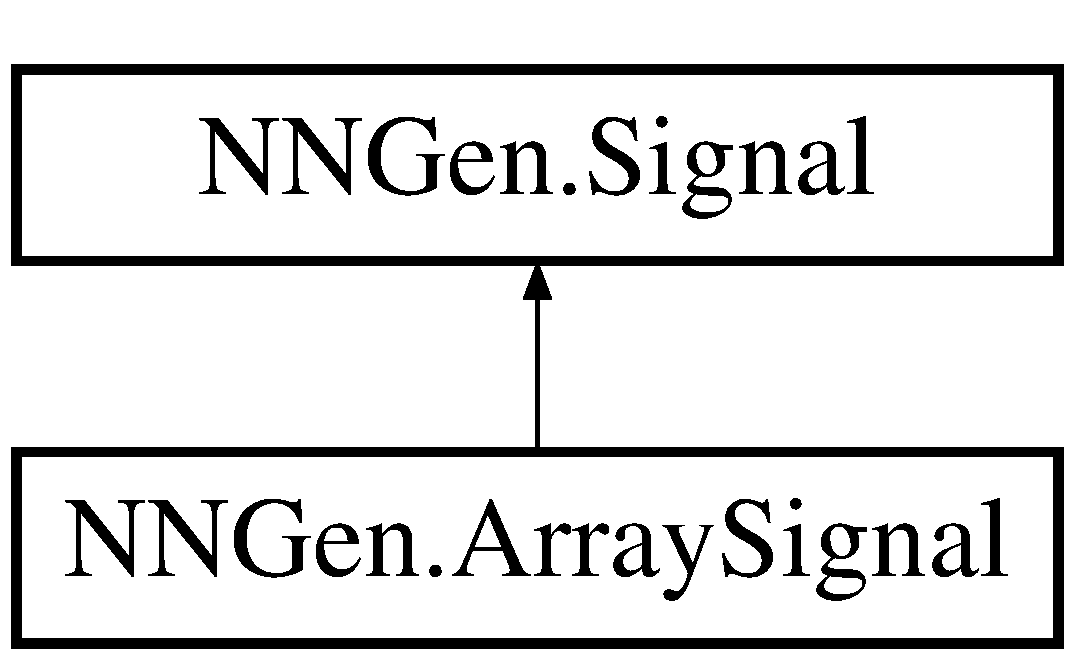
\includegraphics[height=2.000000cm]{class_n_n_gen_1_1_array_signal}
\end{center}
\end{figure}
\subsection*{Public Member Functions}
\begin{DoxyCompactItemize}
\item 
\hyperlink{class_n_n_gen_1_1_array_signal_aee5e895b62756957e013e2993b39ca63}{Array\+Signal} (\hyperlink{class_n_n_gen_1_1_signal}{Signal} \+\_\+base\+Signal, string \+\_\+array\+Name, int \+\_\+array\+Top, int \+\_\+array\+Bottom)
\begin{DoxyCompactList}\small\item\em Creates an array of signals (T\+Y\+P\+E X I\+S A\+R\+R\+A\+Y (Y T\+O Z) O\+F Q) \end{DoxyCompactList}\item 
string \hyperlink{class_n_n_gen_1_1_array_signal_a818715a1024820c7707d338bfcd0f17c}{Declare} ()
\begin{DoxyCompactList}\small\item\em Declares the arry signal type (T\+Y\+P\+E) \end{DoxyCompactList}\item 
override string \hyperlink{class_n_n_gen_1_1_array_signal_a2fa5704a3963a12c2bb188520681a9e6}{V\+H\+D\+L\+String} ()
\begin{DoxyCompactList}\small\item\em Declares the existance of the signal (S\+I\+G\+N\+A\+L) \end{DoxyCompactList}\end{DoxyCompactItemize}
\subsection*{Properties}
\begin{DoxyCompactItemize}
\item 
\hyperlink{class_n_n_gen_1_1_signal}{Signal} \hyperlink{class_n_n_gen_1_1_array_signal_ac02aec9002f01b76184bf49356e73671}{base\+Signal}\hspace{0.3cm}{\ttfamily  \mbox{[}get\mbox{]}}
\begin{DoxyCompactList}\small\item\em The base signal in the array \end{DoxyCompactList}\item 
int \hyperlink{class_n_n_gen_1_1_array_signal_ae5f4cbd20b0ff287422320175a949037}{array\+Top}\hspace{0.3cm}{\ttfamily  \mbox{[}get\mbox{]}}
\begin{DoxyCompactList}\small\item\em The uppper bound of the array (the Y in X T\+O Y) \end{DoxyCompactList}\item 
int \hyperlink{class_n_n_gen_1_1_array_signal_a0c96b2bc754f75aa96537c52ba9d13d1}{array\+Bottom}\hspace{0.3cm}{\ttfamily  \mbox{[}get\mbox{]}}
\begin{DoxyCompactList}\small\item\em The bottom bound of the array (tye X in X T\+O Y) \end{DoxyCompactList}\item 
string \hyperlink{class_n_n_gen_1_1_array_signal_aab7a2cc15c50394e6f6a6085ce467762}{array\+Signal\+Name}\hspace{0.3cm}{\ttfamily  \mbox{[}get\mbox{]}}
\begin{DoxyCompactList}\small\item\em The name of the array \end{DoxyCompactList}\end{DoxyCompactItemize}


\subsection{Detailed Description}
A class to represent an array of signals 



\subsection{Constructor \& Destructor Documentation}
\hypertarget{class_n_n_gen_1_1_array_signal_aee5e895b62756957e013e2993b39ca63}{}\index{N\+N\+Gen\+::\+Array\+Signal@{N\+N\+Gen\+::\+Array\+Signal}!Array\+Signal@{Array\+Signal}}
\index{Array\+Signal@{Array\+Signal}!N\+N\+Gen\+::\+Array\+Signal@{N\+N\+Gen\+::\+Array\+Signal}}
\subsubsection[{Array\+Signal(\+Signal \+\_\+base\+Signal, string \+\_\+array\+Name, int \+\_\+array\+Top, int \+\_\+array\+Bottom)}]{\setlength{\rightskip}{0pt plus 5cm}N\+N\+Gen.\+Array\+Signal.\+Array\+Signal (
\begin{DoxyParamCaption}
\item[{{\bf Signal}}]{\+\_\+base\+Signal, }
\item[{string}]{\+\_\+array\+Name, }
\item[{int}]{\+\_\+array\+Top, }
\item[{int}]{\+\_\+array\+Bottom}
\end{DoxyParamCaption}
)\hspace{0.3cm}{\ttfamily [inline]}}\label{class_n_n_gen_1_1_array_signal_aee5e895b62756957e013e2993b39ca63}


Creates an array of signals (T\+Y\+P\+E X I\+S A\+R\+R\+A\+Y (Y T\+O Z) O\+F Q) 


\begin{DoxyParams}{Parameters}
{\em \+\_\+base\+Signal} & The name of the underlying singal (X)\\
\hline
{\em \+\_\+array\+Name} & The name of the array signal (the name referenced in the S\+I\+G\+N\+A\+L statement)\\
\hline
{\em \+\_\+array\+Top} & The upper limit of the array (Z)\\
\hline
{\em \+\_\+array\+Bottom} & The lower limit of the array (Y)\\
\hline
\end{DoxyParams}


\subsection{Member Function Documentation}
\hypertarget{class_n_n_gen_1_1_array_signal_a818715a1024820c7707d338bfcd0f17c}{}\index{N\+N\+Gen\+::\+Array\+Signal@{N\+N\+Gen\+::\+Array\+Signal}!Declare@{Declare}}
\index{Declare@{Declare}!N\+N\+Gen\+::\+Array\+Signal@{N\+N\+Gen\+::\+Array\+Signal}}
\subsubsection[{Declare()}]{\setlength{\rightskip}{0pt plus 5cm}string N\+N\+Gen.\+Array\+Signal.\+Declare (
\begin{DoxyParamCaption}
{}
\end{DoxyParamCaption}
)\hspace{0.3cm}{\ttfamily [inline]}}\label{class_n_n_gen_1_1_array_signal_a818715a1024820c7707d338bfcd0f17c}


Declares the arry signal type (T\+Y\+P\+E) 

\begin{DoxyReturn}{Returns}

\end{DoxyReturn}
\hypertarget{class_n_n_gen_1_1_array_signal_a2fa5704a3963a12c2bb188520681a9e6}{}\index{N\+N\+Gen\+::\+Array\+Signal@{N\+N\+Gen\+::\+Array\+Signal}!V\+H\+D\+L\+String@{V\+H\+D\+L\+String}}
\index{V\+H\+D\+L\+String@{V\+H\+D\+L\+String}!N\+N\+Gen\+::\+Array\+Signal@{N\+N\+Gen\+::\+Array\+Signal}}
\subsubsection[{V\+H\+D\+L\+String()}]{\setlength{\rightskip}{0pt plus 5cm}override string N\+N\+Gen.\+Array\+Signal.\+V\+H\+D\+L\+String (
\begin{DoxyParamCaption}
{}
\end{DoxyParamCaption}
)\hspace{0.3cm}{\ttfamily [inline]}, {\ttfamily [virtual]}}\label{class_n_n_gen_1_1_array_signal_a2fa5704a3963a12c2bb188520681a9e6}


Declares the existance of the signal (S\+I\+G\+N\+A\+L) 

\begin{DoxyReturn}{Returns}

\end{DoxyReturn}


Reimplemented from \hyperlink{class_n_n_gen_1_1_signal_a35818f3d3a0c4c567701300d90c846ff}{N\+N\+Gen.\+Signal}.



\subsection{Property Documentation}
\hypertarget{class_n_n_gen_1_1_array_signal_a0c96b2bc754f75aa96537c52ba9d13d1}{}\index{N\+N\+Gen\+::\+Array\+Signal@{N\+N\+Gen\+::\+Array\+Signal}!array\+Bottom@{array\+Bottom}}
\index{array\+Bottom@{array\+Bottom}!N\+N\+Gen\+::\+Array\+Signal@{N\+N\+Gen\+::\+Array\+Signal}}
\subsubsection[{array\+Bottom}]{\setlength{\rightskip}{0pt plus 5cm}int N\+N\+Gen.\+Array\+Signal.\+array\+Bottom\hspace{0.3cm}{\ttfamily [get]}}\label{class_n_n_gen_1_1_array_signal_a0c96b2bc754f75aa96537c52ba9d13d1}


The bottom bound of the array (tye X in X T\+O Y) 

\hypertarget{class_n_n_gen_1_1_array_signal_aab7a2cc15c50394e6f6a6085ce467762}{}\index{N\+N\+Gen\+::\+Array\+Signal@{N\+N\+Gen\+::\+Array\+Signal}!array\+Signal\+Name@{array\+Signal\+Name}}
\index{array\+Signal\+Name@{array\+Signal\+Name}!N\+N\+Gen\+::\+Array\+Signal@{N\+N\+Gen\+::\+Array\+Signal}}
\subsubsection[{array\+Signal\+Name}]{\setlength{\rightskip}{0pt plus 5cm}string N\+N\+Gen.\+Array\+Signal.\+array\+Signal\+Name\hspace{0.3cm}{\ttfamily [get]}}\label{class_n_n_gen_1_1_array_signal_aab7a2cc15c50394e6f6a6085ce467762}


The name of the array 

\hypertarget{class_n_n_gen_1_1_array_signal_ae5f4cbd20b0ff287422320175a949037}{}\index{N\+N\+Gen\+::\+Array\+Signal@{N\+N\+Gen\+::\+Array\+Signal}!array\+Top@{array\+Top}}
\index{array\+Top@{array\+Top}!N\+N\+Gen\+::\+Array\+Signal@{N\+N\+Gen\+::\+Array\+Signal}}
\subsubsection[{array\+Top}]{\setlength{\rightskip}{0pt plus 5cm}int N\+N\+Gen.\+Array\+Signal.\+array\+Top\hspace{0.3cm}{\ttfamily [get]}}\label{class_n_n_gen_1_1_array_signal_ae5f4cbd20b0ff287422320175a949037}


The uppper bound of the array (the Y in X T\+O Y) 

\hypertarget{class_n_n_gen_1_1_array_signal_ac02aec9002f01b76184bf49356e73671}{}\index{N\+N\+Gen\+::\+Array\+Signal@{N\+N\+Gen\+::\+Array\+Signal}!base\+Signal@{base\+Signal}}
\index{base\+Signal@{base\+Signal}!N\+N\+Gen\+::\+Array\+Signal@{N\+N\+Gen\+::\+Array\+Signal}}
\subsubsection[{base\+Signal}]{\setlength{\rightskip}{0pt plus 5cm}{\bf Signal} N\+N\+Gen.\+Array\+Signal.\+base\+Signal\hspace{0.3cm}{\ttfamily [get]}}\label{class_n_n_gen_1_1_array_signal_ac02aec9002f01b76184bf49356e73671}


The base signal in the array 



The documentation for this class was generated from the following file\+:\begin{DoxyCompactItemize}
\item 
E\+:/\+Documents/\+Visual Studio 2013/\+Projects/\+Neural\+Network/\+N\+N\+Gen/\hyperlink{_array_signal_8cs}{Array\+Signal.\+cs}\end{DoxyCompactItemize}

\hypertarget{class_n_n_gen_1_1_async_neural_network}{}\section{N\+N\+Gen.\+Async\+Neural\+Network Class Reference}
\label{class_n_n_gen_1_1_async_neural_network}\index{N\+N\+Gen.\+Async\+Neural\+Network@{N\+N\+Gen.\+Async\+Neural\+Network}}


An abstraction of a neural network entity.  


Inheritance diagram for N\+N\+Gen.\+Async\+Neural\+Network\+:\begin{figure}[H]
\begin{center}
\leavevmode
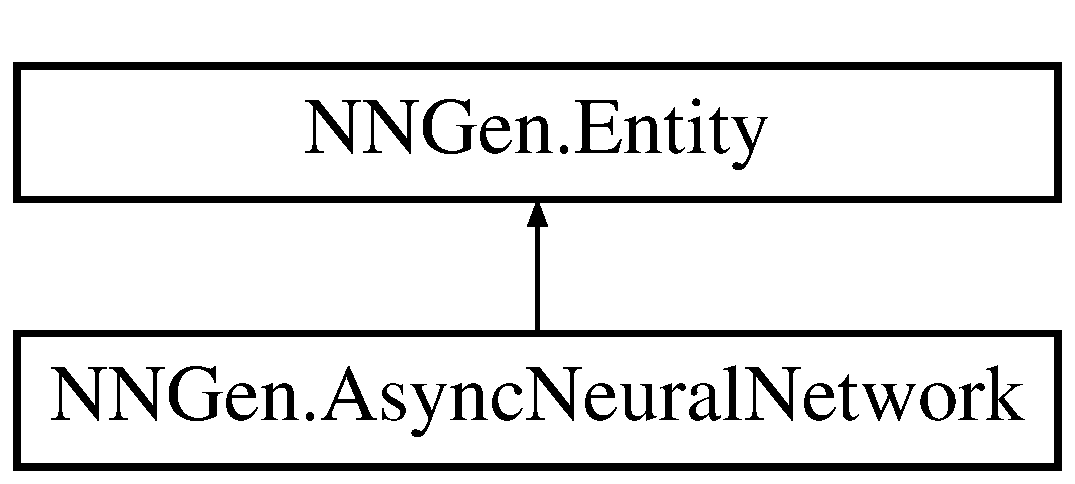
\includegraphics[height=2.000000cm]{class_n_n_gen_1_1_async_neural_network}
\end{center}
\end{figure}
\subsection*{Public Member Functions}
\begin{DoxyCompactItemize}
\item 
\hyperlink{class_n_n_gen_1_1_async_neural_network_ab9139877c5f02159b52437004c5011ac}{Async\+Neural\+Network} (int\mbox{[}$\,$\mbox{]} \+\_\+neuron\+Counts, double\mbox{[}$\,$\mbox{]} \+\_\+bias\+Values, \hyperlink{class_n_n_gen_1_1_async_neuron_afe8460a52808d1587cbcc0a8e4e23b64}{Async\+Neuron.\+Neuron\+Activation\+Type}\mbox{[}$\,$\mbox{]} \+\_\+activation\+Types, int \+\_\+num\+Int\+Bits, int \+\_\+num\+Frac\+Bits, int \+\_\+num\+Weight\+Upper\+Bits, bool \+\_\+is\+Classifier, double\mbox{[}$\,$\mbox{]} \+\_\+classifier\+Thresholds, List$<$ double $>$ \+\_\+weights)
\begin{DoxyCompactList}\small\item\em The constructor for a neural network object. Calling this method\textquotesingle{}s write() function will write the entire network. \end{DoxyCompactList}\item 
override string \hyperlink{class_n_n_gen_1_1_async_neural_network_affd3f3ffb007593e408d63dccf256238}{get\+Name} ()
\begin{DoxyCompactList}\small\item\em Returns the name of the entity. \end{DoxyCompactList}\item 
override \hyperlink{class_n_n_gen_1_1_port}{Port}\mbox{[}$\,$\mbox{]} \hyperlink{class_n_n_gen_1_1_async_neural_network_a94ad9532f7e80514db3ff3eb16ba42cf}{get\+Input\+Ports} ()
\begin{DoxyCompactList}\small\item\em Returns the input ports of the entity. \end{DoxyCompactList}\item 
override \hyperlink{class_n_n_gen_1_1_port}{Port}\mbox{[}$\,$\mbox{]} \hyperlink{class_n_n_gen_1_1_async_neural_network_a1efde159a323347b01cd88527d61c14e}{get\+Output\+Ports} ()
\begin{DoxyCompactList}\small\item\em Returns the output ports of the entity. \end{DoxyCompactList}\item 
override \hyperlink{class_n_n_gen_1_1_signal}{Signal}\mbox{[}$\,$\mbox{]} \hyperlink{class_n_n_gen_1_1_async_neural_network_a4ef8c71674da4a162680bf5b5c22d928}{get\+Internal\+Signals} ()
\begin{DoxyCompactList}\small\item\em Returns the internal signals of the entity. \end{DoxyCompactList}\item 
override bool \hyperlink{class_n_n_gen_1_1_async_neural_network_ad57a90889256277e0da34e8e7f3e7848}{write\+V\+H\+D\+L} (string file)
\begin{DoxyCompactList}\small\item\em Writes the .vhd files necessary to compile this entity. All other necessary entities (i.\+e. neurons, thresholding functions, etc.) will also be written when this function returns \end{DoxyCompactList}\end{DoxyCompactItemize}
\subsection*{Properties}
\begin{DoxyCompactItemize}
\item 
\hyperlink{class_n_n_gen_1_1_port}{Port}\mbox{[}$\,$\mbox{]} \hyperlink{class_n_n_gen_1_1_async_neural_network_a6422fde806a9cf2188ca93c5166ebb23}{nn\+Input\+Ports}\hspace{0.3cm}{\ttfamily  \mbox{[}get\mbox{]}}
\begin{DoxyCompactList}\small\item\em The list of input ports to the network \end{DoxyCompactList}\item 
\hyperlink{class_n_n_gen_1_1_port}{Port}\mbox{[}$\,$\mbox{]} \hyperlink{class_n_n_gen_1_1_async_neural_network_a666078677fa5db12619f912ca472bdee}{nn\+Output\+Ports}\hspace{0.3cm}{\ttfamily  \mbox{[}get\mbox{]}}
\begin{DoxyCompactList}\small\item\em The list of output ports to the network \end{DoxyCompactList}\item 
\hyperlink{class_n_n_gen_1_1_port}{Port} \hyperlink{class_n_n_gen_1_1_async_neural_network_a30cb0df931a8da4dd7e911f953caaf02}{ready}\hspace{0.3cm}{\ttfamily  \mbox{[}get\mbox{]}}
\begin{DoxyCompactList}\small\item\em This signal will go high when the network has been initialized after a reset. It will go low when the device is in reset \end{DoxyCompactList}\item 
\hyperlink{class_n_n_gen_1_1_port}{Port} \hyperlink{class_n_n_gen_1_1_async_neural_network_ad3bb38686daf90675f37c81e6b8e749e}{clk}\hspace{0.3cm}{\ttfamily  \mbox{[}get\mbox{]}}
\begin{DoxyCompactList}\small\item\em A clock used for synchronous loading of the neuron weights from memory \end{DoxyCompactList}\item 
\hyperlink{class_n_n_gen_1_1_port}{Port} \hyperlink{class_n_n_gen_1_1_async_neural_network_a7205fb71714f4aa3c144c72c44af2787}{reset}\hspace{0.3cm}{\ttfamily  \mbox{[}get\mbox{]}}
\begin{DoxyCompactList}\small\item\em An active high reset for the network \end{DoxyCompactList}\item 
\hyperlink{class_n_n_gen_1_1_async_neuron_afe8460a52808d1587cbcc0a8e4e23b64}{Async\+Neuron.\+Neuron\+Activation\+Type}\mbox{[}$\,$\mbox{]} \hyperlink{class_n_n_gen_1_1_async_neural_network_ad1d4a0489b5e32e36e8927eee2992725}{activation\+Types}\hspace{0.3cm}{\ttfamily  \mbox{[}get\mbox{]}}
\begin{DoxyCompactList}\small\item\em The activation types for each layer of the network. The i-\/th member corresponds to the activations of the i-\/th layer of the network \end{DoxyCompactList}\item 
int\mbox{[}$\,$\mbox{]} \hyperlink{class_n_n_gen_1_1_async_neural_network_aec2195cbfa8c8f568dc512ab511d06c0}{neuron\+Counts}\hspace{0.3cm}{\ttfamily  \mbox{[}get\mbox{]}}
\begin{DoxyCompactList}\small\item\em The number of neurons in each layer of the network. The i-\/th member corresponds to the i-\/th layer of the network \end{DoxyCompactList}\item 
double\mbox{[}$\,$\mbox{]} \hyperlink{class_n_n_gen_1_1_async_neural_network_aaccc75ccaaf278324874a5c3b45d711f}{bias\+Values}\hspace{0.3cm}{\ttfamily  \mbox{[}get\mbox{]}}
\begin{DoxyCompactList}\small\item\em The bias values for each layer. The i-\/th member corresponds to the bias value fed into the i+1-\/th layer of the network \end{DoxyCompactList}\item 
\hyperlink{class_n_n_gen_1_1_signal}{Signal} \hyperlink{class_n_n_gen_1_1_async_neural_network_a4bb7830d6bbc7f19ea5eefdb49ab848a}{load\+\_\+sig}\hspace{0.3cm}{\ttfamily  \mbox{[}get\mbox{]}}
\begin{DoxyCompactList}\small\item\em A signal used to enable a single neuron to accept weights from memory \end{DoxyCompactList}\item 
\hyperlink{class_n_n_gen_1_1_signal}{Signal} \hyperlink{class_n_n_gen_1_1_async_neural_network_aced8cd708a7084592d28cbcca93a7278}{load\+Val}\hspace{0.3cm}{\ttfamily  \mbox{[}get\mbox{]}}
\begin{DoxyCompactList}\small\item\em A signal to hold the values of data coming from memory \end{DoxyCompactList}\item 
\hyperlink{class_n_n_gen_1_1_signal}{Signal} \hyperlink{class_n_n_gen_1_1_async_neural_network_aedc34ca8e8b46a154d3953776c809cd9}{load\+Offset}\hspace{0.3cm}{\ttfamily  \mbox{[}get\mbox{]}}
\begin{DoxyCompactList}\small\item\em A signal used to index into an individual neuron\textquotesingle{}s weight signals Used during the load process \end{DoxyCompactList}\item 
\hyperlink{class_n_n_gen_1_1_signal}{Signal} \hyperlink{class_n_n_gen_1_1_async_neural_network_a62f80368a823158ee82fd29b879ad157}{addr\+Counter}\hspace{0.3cm}{\ttfamily  \mbox{[}get\mbox{]}}
\begin{DoxyCompactList}\small\item\em A signal used to index into memory to obtain the weights during the load process \end{DoxyCompactList}\item 
\hyperlink{class_n_n_gen_1_1_signal}{Signal}\mbox{[}$\,$\mbox{]} \hyperlink{class_n_n_gen_1_1_async_neural_network_ac912fc0d486aeb193cf0f104f06b68a4}{neuron\+\_\+outputs}\hspace{0.3cm}{\ttfamily  \mbox{[}get\mbox{]}}
\begin{DoxyCompactList}\small\item\em The signals that will hold the outputs to each individual neuron \end{DoxyCompactList}\item 
\hyperlink{class_n_n_gen_1_1_signal}{Signal} \hyperlink{class_n_n_gen_1_1_async_neural_network_ade446cacb56d0ddf2aae1510e2425591}{ready\+\_\+signal}\hspace{0.3cm}{\ttfamily  \mbox{[}get\mbox{]}}
\begin{DoxyCompactList}\small\item\em A signal used in determining whether the device has completed the loading process \end{DoxyCompactList}\item 
\hyperlink{class_n_n_gen_1_1_signal}{Signal}\mbox{[}$\,$\mbox{]} \hyperlink{class_n_n_gen_1_1_async_neural_network_a17ce3ebd6db5f93a473bd2b45527c726}{final\+Load\+Signals}\hspace{0.3cm}{\ttfamily  \mbox{[}get\mbox{]}}
\begin{DoxyCompactList}\small\item\em A collection of signals to hold the final\+\_\+load outputs from the individual neurons in the network \end{DoxyCompactList}\item 
\hyperlink{class_n_n_gen_1_1_signal}{Signal} \hyperlink{class_n_n_gen_1_1_async_neural_network_a559b0be95e6e62b80a0064de584805d3}{load\+Val\+Conv}\hspace{0.3cm}{\ttfamily  \mbox{[}get\mbox{]}}
\begin{DoxyCompactList}\small\item\em A signal used to convert the output of memory (S\+T\+D\+\_\+\+L\+O\+G\+I\+C\+\_\+\+V\+E\+C\+T\+O\+R) into the appropriate type to be used in the neuron (S\+I\+G\+N\+E\+D\+\_\+\+F\+I\+X\+E\+D\+\_\+\+P\+O\+I\+N\+T) \end{DoxyCompactList}\item 
double\mbox{[}$\,$\mbox{]} \hyperlink{class_n_n_gen_1_1_async_neural_network_a9a2da98105807d64bf8d25f9f4279d3f}{classifier\+Thresholds}\hspace{0.3cm}{\ttfamily  \mbox{[}get\mbox{]}}
\begin{DoxyCompactList}\small\item\em The values to be used for thresholding the output neurons. The i-\/th member of this array corresponds to the theshold value for the i-\/th output neuron. If the network is not a classification network (i.\+e. is\+Classifier = false), then this member is unused. \end{DoxyCompactList}\item 
bool \hyperlink{class_n_n_gen_1_1_async_neural_network_a07f0f12e804555587a5869b821e2ab0f}{is\+Classifier}\hspace{0.3cm}{\ttfamily  \mbox{[}get\mbox{]}}
\begin{DoxyCompactList}\small\item\em If the neural network is to be used for classification, then this variable should be set to true. This will instantiate comparitors on the output neurons. \end{DoxyCompactList}\item 
int \hyperlink{class_n_n_gen_1_1_async_neural_network_aa792285911d8e4b6d402451efe7d57c2}{num\+Int\+Bits}\hspace{0.3cm}{\ttfamily  \mbox{[}get\mbox{]}}
\begin{DoxyCompactList}\small\item\em The number of integer bits to be used for the neural network inputs \end{DoxyCompactList}\item 
int \hyperlink{class_n_n_gen_1_1_async_neural_network_a195b5331d3ed6f5babecb6e7e6b22cb7}{num\+Frac\+Bits}\hspace{0.3cm}{\ttfamily  \mbox{[}get\mbox{]}}
\begin{DoxyCompactList}\small\item\em The number of fractional bits to be used for the neural network inputs and for the neural network weights \end{DoxyCompactList}\item 
int \hyperlink{class_n_n_gen_1_1_async_neural_network_a098bee8b58e461ea1141e5a2c165ee88}{num\+Weight\+Upper\+Bits}\hspace{0.3cm}{\ttfamily  \mbox{[}get\mbox{]}}
\begin{DoxyCompactList}\small\item\em The number of integer bits to be used for the neural network weights. \end{DoxyCompactList}\item 
\hyperlink{class_n_n_gen_1_1_weight_memory}{Weight\+Memory} \hyperlink{class_n_n_gen_1_1_async_neural_network_a94241380da2839193000b7c3e78fe8cd}{wm}\hspace{0.3cm}{\ttfamily  \mbox{[}get\mbox{]}}
\begin{DoxyCompactList}\small\item\em A memory entity used to store and load the neural network weights on startup \end{DoxyCompactList}\item 
\hyperlink{class_n_n_gen_1_1_async_neuron}{Async\+Neuron}\mbox{[}$\,$\mbox{]} \hyperlink{class_n_n_gen_1_1_async_neural_network_aeaec2eb4cfb3a7dba9c40d04c2fe7fb1}{neuron\+Entities}\hspace{0.3cm}{\ttfamily  \mbox{[}get\mbox{]}}
\begin{DoxyCompactList}\small\item\em An array of the neurons in the network. It is sequentually loaded, first by layer, then by order within the layer. So, for a net of N layers, each with M neurons in the layer, the array will be \mbox{[}Neuron\+\_\+0\+\_\+0, Neuron\+\_\+0\+\_\+1, ..., Neuron\+\_\+0\+\_\+\+M, Neuron\+\_\+1\+\_\+0, Neuron\+\_\+1\+\_\+1, ..., Neuron\+\_\+\+N\+\_\+\+M\mbox{]} \end{DoxyCompactList}\item 
List$<$ \hyperlink{class_n_n_gen_1_1_async_neuron}{Async\+Neuron} $>$ \hyperlink{class_n_n_gen_1_1_async_neural_network_a0f6322f9b2736a40e4f63b3107f8981d}{unique\+Neuron\+Entities}\hspace{0.3cm}{\ttfamily  \mbox{[}get\mbox{]}}
\begin{DoxyCompactList}\small\item\em A list of the unique neuron entities for which separate V\+H\+D\+L files will need to be generated. \end{DoxyCompactList}\item 
int\mbox{[}$\,$\mbox{]} \hyperlink{class_n_n_gen_1_1_async_neural_network_a545f2bfc72b27d96c054de93d82a7571}{int\+Bus\+Widths}\hspace{0.3cm}{\ttfamily  \mbox{[}get\mbox{]}}
\begin{DoxyCompactList}\small\item\em The bus widths for each neuron \end{DoxyCompactList}\end{DoxyCompactItemize}


\subsection{Detailed Description}
An abstraction of a neural network entity. 



\subsection{Constructor \& Destructor Documentation}
\hypertarget{class_n_n_gen_1_1_async_neural_network_ab9139877c5f02159b52437004c5011ac}{}\index{N\+N\+Gen\+::\+Async\+Neural\+Network@{N\+N\+Gen\+::\+Async\+Neural\+Network}!Async\+Neural\+Network@{Async\+Neural\+Network}}
\index{Async\+Neural\+Network@{Async\+Neural\+Network}!N\+N\+Gen\+::\+Async\+Neural\+Network@{N\+N\+Gen\+::\+Async\+Neural\+Network}}
\subsubsection[{Async\+Neural\+Network(int[] \+\_\+neuron\+Counts, double[] \+\_\+bias\+Values, Async\+Neuron.\+Neuron\+Activation\+Type[] \+\_\+activation\+Types, int \+\_\+num\+Int\+Bits, int \+\_\+num\+Frac\+Bits, int \+\_\+num\+Weight\+Upper\+Bits, bool \+\_\+is\+Classifier, double[] \+\_\+classifier\+Thresholds, List$<$ double $>$ \+\_\+weights)}]{\setlength{\rightskip}{0pt plus 5cm}N\+N\+Gen.\+Async\+Neural\+Network.\+Async\+Neural\+Network (
\begin{DoxyParamCaption}
\item[{int\mbox{[}$\,$\mbox{]}}]{\+\_\+neuron\+Counts, }
\item[{double\mbox{[}$\,$\mbox{]}}]{\+\_\+bias\+Values, }
\item[{{\bf Async\+Neuron.\+Neuron\+Activation\+Type}\mbox{[}$\,$\mbox{]}}]{\+\_\+activation\+Types, }
\item[{int}]{\+\_\+num\+Int\+Bits, }
\item[{int}]{\+\_\+num\+Frac\+Bits, }
\item[{int}]{\+\_\+num\+Weight\+Upper\+Bits, }
\item[{bool}]{\+\_\+is\+Classifier, }
\item[{double\mbox{[}$\,$\mbox{]}}]{\+\_\+classifier\+Thresholds, }
\item[{List$<$ double $>$}]{\+\_\+weights}
\end{DoxyParamCaption}
)\hspace{0.3cm}{\ttfamily [inline]}}\label{class_n_n_gen_1_1_async_neural_network_ab9139877c5f02159b52437004c5011ac}


The constructor for a neural network object. Calling this method\textquotesingle{}s write() function will write the entire network. 


\begin{DoxyParams}{Parameters}
{\em \+\_\+neuron\+Counts} & The number of neurons in each layer, excluding the bias node.\\
\hline
{\em \+\_\+bias\+Values} & The bias value feeding forward into the next layer. \\
\hline
{\em \+\_\+activation\+Types} & The activation types for the neurons in each layer\\
\hline
{\em \+\_\+num\+Int\+Bits} & The number of integer bits to use for the inputs for each neuron (Sigmoid activated neurons automatically get this set to zero)\\
\hline
{\em \+\_\+num\+Frac\+Bits} & The number of fractional bits to use for the inputs for each neuron\\
\hline
{\em \+\_\+num\+Weight\+Upper\+Bits} & The number of integer bits used for the weights for each neuron.\\
\hline
{\em \+\_\+is\+Classifier} & If true, a comparitor will be instantiatated at the output to each node, comparing the output layer nodes to the threshold value.\\
\hline
{\em \+\_\+classifier\+Thresholds} & The threshold values for the output comparitors\\
\hline
{\em \+\_\+weights} & The list of weights read in for the neurons from Weight\+Reader.\+read\+Weights\+From\+File()\\
\hline
\end{DoxyParams}
$<$remark$>$ For example, to intialize a classification neural network with three inputs, two hidden sigmoid-\/activated nodes, and one linear output node, use the following line\+:$<$/remark$>$ 

Neural\+Network nn = new Neural\+Network(\mbox{[}3, 2, 1\mbox{]}, \mbox{[}-\/1, -\/1\mbox{]}, \mbox{[}..S\+I\+G\+M\+O\+I\+D\+\_\+\+P\+O\+L\+Y\+\_\+\+A\+P\+P\+R\+O\+X, ..L\+I\+N\+E\+A\+R\mbox{]}, 4, 4, 4, true, \mbox{[}0.\+5\mbox{]}, \+\_\+weights);

\subsection{Member Function Documentation}
\hypertarget{class_n_n_gen_1_1_async_neural_network_a94ad9532f7e80514db3ff3eb16ba42cf}{}\index{N\+N\+Gen\+::\+Async\+Neural\+Network@{N\+N\+Gen\+::\+Async\+Neural\+Network}!get\+Input\+Ports@{get\+Input\+Ports}}
\index{get\+Input\+Ports@{get\+Input\+Ports}!N\+N\+Gen\+::\+Async\+Neural\+Network@{N\+N\+Gen\+::\+Async\+Neural\+Network}}
\subsubsection[{get\+Input\+Ports()}]{\setlength{\rightskip}{0pt plus 5cm}override {\bf Port} \mbox{[}$\,$\mbox{]} N\+N\+Gen.\+Async\+Neural\+Network.\+get\+Input\+Ports (
\begin{DoxyParamCaption}
{}
\end{DoxyParamCaption}
)\hspace{0.3cm}{\ttfamily [inline]}, {\ttfamily [virtual]}}\label{class_n_n_gen_1_1_async_neural_network_a94ad9532f7e80514db3ff3eb16ba42cf}


Returns the input ports of the entity. 

\begin{DoxyReturn}{Returns}
The input ports of the entity
\end{DoxyReturn}


Implements \hyperlink{class_n_n_gen_1_1_entity_a01239f05c9efa61ec9e6a29cb2eaad50}{N\+N\+Gen.\+Entity}.

\hypertarget{class_n_n_gen_1_1_async_neural_network_a4ef8c71674da4a162680bf5b5c22d928}{}\index{N\+N\+Gen\+::\+Async\+Neural\+Network@{N\+N\+Gen\+::\+Async\+Neural\+Network}!get\+Internal\+Signals@{get\+Internal\+Signals}}
\index{get\+Internal\+Signals@{get\+Internal\+Signals}!N\+N\+Gen\+::\+Async\+Neural\+Network@{N\+N\+Gen\+::\+Async\+Neural\+Network}}
\subsubsection[{get\+Internal\+Signals()}]{\setlength{\rightskip}{0pt plus 5cm}override {\bf Signal} \mbox{[}$\,$\mbox{]} N\+N\+Gen.\+Async\+Neural\+Network.\+get\+Internal\+Signals (
\begin{DoxyParamCaption}
{}
\end{DoxyParamCaption}
)\hspace{0.3cm}{\ttfamily [inline]}, {\ttfamily [virtual]}}\label{class_n_n_gen_1_1_async_neural_network_a4ef8c71674da4a162680bf5b5c22d928}


Returns the internal signals of the entity. 

\begin{DoxyReturn}{Returns}
The internal signals of the entity
\end{DoxyReturn}


Implements \hyperlink{class_n_n_gen_1_1_entity_a62feb80e95ec84c650ea17bd53f0d510}{N\+N\+Gen.\+Entity}.

\hypertarget{class_n_n_gen_1_1_async_neural_network_affd3f3ffb007593e408d63dccf256238}{}\index{N\+N\+Gen\+::\+Async\+Neural\+Network@{N\+N\+Gen\+::\+Async\+Neural\+Network}!get\+Name@{get\+Name}}
\index{get\+Name@{get\+Name}!N\+N\+Gen\+::\+Async\+Neural\+Network@{N\+N\+Gen\+::\+Async\+Neural\+Network}}
\subsubsection[{get\+Name()}]{\setlength{\rightskip}{0pt plus 5cm}override string N\+N\+Gen.\+Async\+Neural\+Network.\+get\+Name (
\begin{DoxyParamCaption}
{}
\end{DoxyParamCaption}
)\hspace{0.3cm}{\ttfamily [inline]}, {\ttfamily [virtual]}}\label{class_n_n_gen_1_1_async_neural_network_affd3f3ffb007593e408d63dccf256238}


Returns the name of the entity. 

\begin{DoxyReturn}{Returns}
The name of the entity
\end{DoxyReturn}


Implements \hyperlink{class_n_n_gen_1_1_entity_a9f25d1070c9ab8ad343c28443e62e6f2}{N\+N\+Gen.\+Entity}.

\hypertarget{class_n_n_gen_1_1_async_neural_network_a1efde159a323347b01cd88527d61c14e}{}\index{N\+N\+Gen\+::\+Async\+Neural\+Network@{N\+N\+Gen\+::\+Async\+Neural\+Network}!get\+Output\+Ports@{get\+Output\+Ports}}
\index{get\+Output\+Ports@{get\+Output\+Ports}!N\+N\+Gen\+::\+Async\+Neural\+Network@{N\+N\+Gen\+::\+Async\+Neural\+Network}}
\subsubsection[{get\+Output\+Ports()}]{\setlength{\rightskip}{0pt plus 5cm}override {\bf Port} \mbox{[}$\,$\mbox{]} N\+N\+Gen.\+Async\+Neural\+Network.\+get\+Output\+Ports (
\begin{DoxyParamCaption}
{}
\end{DoxyParamCaption}
)\hspace{0.3cm}{\ttfamily [inline]}, {\ttfamily [virtual]}}\label{class_n_n_gen_1_1_async_neural_network_a1efde159a323347b01cd88527d61c14e}


Returns the output ports of the entity. 

\begin{DoxyReturn}{Returns}
The output ports of the entity
\end{DoxyReturn}


Implements \hyperlink{class_n_n_gen_1_1_entity_ace06368087778e254a5048c7d28747be}{N\+N\+Gen.\+Entity}.

\hypertarget{class_n_n_gen_1_1_async_neural_network_ad57a90889256277e0da34e8e7f3e7848}{}\index{N\+N\+Gen\+::\+Async\+Neural\+Network@{N\+N\+Gen\+::\+Async\+Neural\+Network}!write\+V\+H\+D\+L@{write\+V\+H\+D\+L}}
\index{write\+V\+H\+D\+L@{write\+V\+H\+D\+L}!N\+N\+Gen\+::\+Async\+Neural\+Network@{N\+N\+Gen\+::\+Async\+Neural\+Network}}
\subsubsection[{write\+V\+H\+D\+L(string file)}]{\setlength{\rightskip}{0pt plus 5cm}override bool N\+N\+Gen.\+Async\+Neural\+Network.\+write\+V\+H\+D\+L (
\begin{DoxyParamCaption}
\item[{string}]{file}
\end{DoxyParamCaption}
)\hspace{0.3cm}{\ttfamily [inline]}, {\ttfamily [virtual]}}\label{class_n_n_gen_1_1_async_neural_network_ad57a90889256277e0da34e8e7f3e7848}


Writes the .vhd files necessary to compile this entity. All other necessary entities (i.\+e. neurons, thresholding functions, etc.) will also be written when this function returns 


\begin{DoxyParams}{Parameters}
{\em file} & The file path in which to write the files (do N\+O\+T include \char`\"{}...\+name.\+vhd\char`\"{}\\
\hline
\end{DoxyParams}
\begin{DoxyReturn}{Returns}
true if the files were written successfully, false otherwise
\end{DoxyReturn}


Implements \hyperlink{class_n_n_gen_1_1_entity_a1111d498446be08b20583b9625893a52}{N\+N\+Gen.\+Entity}.



\subsection{Property Documentation}
\hypertarget{class_n_n_gen_1_1_async_neural_network_ad1d4a0489b5e32e36e8927eee2992725}{}\index{N\+N\+Gen\+::\+Async\+Neural\+Network@{N\+N\+Gen\+::\+Async\+Neural\+Network}!activation\+Types@{activation\+Types}}
\index{activation\+Types@{activation\+Types}!N\+N\+Gen\+::\+Async\+Neural\+Network@{N\+N\+Gen\+::\+Async\+Neural\+Network}}
\subsubsection[{activation\+Types}]{\setlength{\rightskip}{0pt plus 5cm}{\bf Async\+Neuron.\+Neuron\+Activation\+Type} \mbox{[}$\,$\mbox{]} N\+N\+Gen.\+Async\+Neural\+Network.\+activation\+Types\hspace{0.3cm}{\ttfamily [get]}}\label{class_n_n_gen_1_1_async_neural_network_ad1d4a0489b5e32e36e8927eee2992725}


The activation types for each layer of the network. The i-\/th member corresponds to the activations of the i-\/th layer of the network 

\hypertarget{class_n_n_gen_1_1_async_neural_network_a62f80368a823158ee82fd29b879ad157}{}\index{N\+N\+Gen\+::\+Async\+Neural\+Network@{N\+N\+Gen\+::\+Async\+Neural\+Network}!addr\+Counter@{addr\+Counter}}
\index{addr\+Counter@{addr\+Counter}!N\+N\+Gen\+::\+Async\+Neural\+Network@{N\+N\+Gen\+::\+Async\+Neural\+Network}}
\subsubsection[{addr\+Counter}]{\setlength{\rightskip}{0pt plus 5cm}{\bf Signal} N\+N\+Gen.\+Async\+Neural\+Network.\+addr\+Counter\hspace{0.3cm}{\ttfamily [get]}}\label{class_n_n_gen_1_1_async_neural_network_a62f80368a823158ee82fd29b879ad157}


A signal used to index into memory to obtain the weights during the load process 

\hypertarget{class_n_n_gen_1_1_async_neural_network_aaccc75ccaaf278324874a5c3b45d711f}{}\index{N\+N\+Gen\+::\+Async\+Neural\+Network@{N\+N\+Gen\+::\+Async\+Neural\+Network}!bias\+Values@{bias\+Values}}
\index{bias\+Values@{bias\+Values}!N\+N\+Gen\+::\+Async\+Neural\+Network@{N\+N\+Gen\+::\+Async\+Neural\+Network}}
\subsubsection[{bias\+Values}]{\setlength{\rightskip}{0pt plus 5cm}double \mbox{[}$\,$\mbox{]} N\+N\+Gen.\+Async\+Neural\+Network.\+bias\+Values\hspace{0.3cm}{\ttfamily [get]}}\label{class_n_n_gen_1_1_async_neural_network_aaccc75ccaaf278324874a5c3b45d711f}


The bias values for each layer. The i-\/th member corresponds to the bias value fed into the i+1-\/th layer of the network 

\hypertarget{class_n_n_gen_1_1_async_neural_network_a9a2da98105807d64bf8d25f9f4279d3f}{}\index{N\+N\+Gen\+::\+Async\+Neural\+Network@{N\+N\+Gen\+::\+Async\+Neural\+Network}!classifier\+Thresholds@{classifier\+Thresholds}}
\index{classifier\+Thresholds@{classifier\+Thresholds}!N\+N\+Gen\+::\+Async\+Neural\+Network@{N\+N\+Gen\+::\+Async\+Neural\+Network}}
\subsubsection[{classifier\+Thresholds}]{\setlength{\rightskip}{0pt plus 5cm}double \mbox{[}$\,$\mbox{]} N\+N\+Gen.\+Async\+Neural\+Network.\+classifier\+Thresholds\hspace{0.3cm}{\ttfamily [get]}}\label{class_n_n_gen_1_1_async_neural_network_a9a2da98105807d64bf8d25f9f4279d3f}


The values to be used for thresholding the output neurons. The i-\/th member of this array corresponds to the theshold value for the i-\/th output neuron. If the network is not a classification network (i.\+e. is\+Classifier = false), then this member is unused. 

\hypertarget{class_n_n_gen_1_1_async_neural_network_ad3bb38686daf90675f37c81e6b8e749e}{}\index{N\+N\+Gen\+::\+Async\+Neural\+Network@{N\+N\+Gen\+::\+Async\+Neural\+Network}!clk@{clk}}
\index{clk@{clk}!N\+N\+Gen\+::\+Async\+Neural\+Network@{N\+N\+Gen\+::\+Async\+Neural\+Network}}
\subsubsection[{clk}]{\setlength{\rightskip}{0pt plus 5cm}{\bf Port} N\+N\+Gen.\+Async\+Neural\+Network.\+clk\hspace{0.3cm}{\ttfamily [get]}}\label{class_n_n_gen_1_1_async_neural_network_ad3bb38686daf90675f37c81e6b8e749e}


A clock used for synchronous loading of the neuron weights from memory 

\hypertarget{class_n_n_gen_1_1_async_neural_network_a17ce3ebd6db5f93a473bd2b45527c726}{}\index{N\+N\+Gen\+::\+Async\+Neural\+Network@{N\+N\+Gen\+::\+Async\+Neural\+Network}!final\+Load\+Signals@{final\+Load\+Signals}}
\index{final\+Load\+Signals@{final\+Load\+Signals}!N\+N\+Gen\+::\+Async\+Neural\+Network@{N\+N\+Gen\+::\+Async\+Neural\+Network}}
\subsubsection[{final\+Load\+Signals}]{\setlength{\rightskip}{0pt plus 5cm}{\bf Signal} \mbox{[}$\,$\mbox{]} N\+N\+Gen.\+Async\+Neural\+Network.\+final\+Load\+Signals\hspace{0.3cm}{\ttfamily [get]}}\label{class_n_n_gen_1_1_async_neural_network_a17ce3ebd6db5f93a473bd2b45527c726}


A collection of signals to hold the final\+\_\+load outputs from the individual neurons in the network 

\hypertarget{class_n_n_gen_1_1_async_neural_network_a545f2bfc72b27d96c054de93d82a7571}{}\index{N\+N\+Gen\+::\+Async\+Neural\+Network@{N\+N\+Gen\+::\+Async\+Neural\+Network}!int\+Bus\+Widths@{int\+Bus\+Widths}}
\index{int\+Bus\+Widths@{int\+Bus\+Widths}!N\+N\+Gen\+::\+Async\+Neural\+Network@{N\+N\+Gen\+::\+Async\+Neural\+Network}}
\subsubsection[{int\+Bus\+Widths}]{\setlength{\rightskip}{0pt plus 5cm}int \mbox{[}$\,$\mbox{]} N\+N\+Gen.\+Async\+Neural\+Network.\+int\+Bus\+Widths\hspace{0.3cm}{\ttfamily [get]}}\label{class_n_n_gen_1_1_async_neural_network_a545f2bfc72b27d96c054de93d82a7571}


The bus widths for each neuron 

\hypertarget{class_n_n_gen_1_1_async_neural_network_a07f0f12e804555587a5869b821e2ab0f}{}\index{N\+N\+Gen\+::\+Async\+Neural\+Network@{N\+N\+Gen\+::\+Async\+Neural\+Network}!is\+Classifier@{is\+Classifier}}
\index{is\+Classifier@{is\+Classifier}!N\+N\+Gen\+::\+Async\+Neural\+Network@{N\+N\+Gen\+::\+Async\+Neural\+Network}}
\subsubsection[{is\+Classifier}]{\setlength{\rightskip}{0pt plus 5cm}bool N\+N\+Gen.\+Async\+Neural\+Network.\+is\+Classifier\hspace{0.3cm}{\ttfamily [get]}}\label{class_n_n_gen_1_1_async_neural_network_a07f0f12e804555587a5869b821e2ab0f}


If the neural network is to be used for classification, then this variable should be set to true. This will instantiate comparitors on the output neurons. 

\hypertarget{class_n_n_gen_1_1_async_neural_network_a4bb7830d6bbc7f19ea5eefdb49ab848a}{}\index{N\+N\+Gen\+::\+Async\+Neural\+Network@{N\+N\+Gen\+::\+Async\+Neural\+Network}!load\+\_\+sig@{load\+\_\+sig}}
\index{load\+\_\+sig@{load\+\_\+sig}!N\+N\+Gen\+::\+Async\+Neural\+Network@{N\+N\+Gen\+::\+Async\+Neural\+Network}}
\subsubsection[{load\+\_\+sig}]{\setlength{\rightskip}{0pt plus 5cm}{\bf Signal} N\+N\+Gen.\+Async\+Neural\+Network.\+load\+\_\+sig\hspace{0.3cm}{\ttfamily [get]}}\label{class_n_n_gen_1_1_async_neural_network_a4bb7830d6bbc7f19ea5eefdb49ab848a}


A signal used to enable a single neuron to accept weights from memory 

\hypertarget{class_n_n_gen_1_1_async_neural_network_aedc34ca8e8b46a154d3953776c809cd9}{}\index{N\+N\+Gen\+::\+Async\+Neural\+Network@{N\+N\+Gen\+::\+Async\+Neural\+Network}!load\+Offset@{load\+Offset}}
\index{load\+Offset@{load\+Offset}!N\+N\+Gen\+::\+Async\+Neural\+Network@{N\+N\+Gen\+::\+Async\+Neural\+Network}}
\subsubsection[{load\+Offset}]{\setlength{\rightskip}{0pt plus 5cm}{\bf Signal} N\+N\+Gen.\+Async\+Neural\+Network.\+load\+Offset\hspace{0.3cm}{\ttfamily [get]}}\label{class_n_n_gen_1_1_async_neural_network_aedc34ca8e8b46a154d3953776c809cd9}


A signal used to index into an individual neuron\textquotesingle{}s weight signals Used during the load process 

\hypertarget{class_n_n_gen_1_1_async_neural_network_aced8cd708a7084592d28cbcca93a7278}{}\index{N\+N\+Gen\+::\+Async\+Neural\+Network@{N\+N\+Gen\+::\+Async\+Neural\+Network}!load\+Val@{load\+Val}}
\index{load\+Val@{load\+Val}!N\+N\+Gen\+::\+Async\+Neural\+Network@{N\+N\+Gen\+::\+Async\+Neural\+Network}}
\subsubsection[{load\+Val}]{\setlength{\rightskip}{0pt plus 5cm}{\bf Signal} N\+N\+Gen.\+Async\+Neural\+Network.\+load\+Val\hspace{0.3cm}{\ttfamily [get]}}\label{class_n_n_gen_1_1_async_neural_network_aced8cd708a7084592d28cbcca93a7278}


A signal to hold the values of data coming from memory 

\hypertarget{class_n_n_gen_1_1_async_neural_network_a559b0be95e6e62b80a0064de584805d3}{}\index{N\+N\+Gen\+::\+Async\+Neural\+Network@{N\+N\+Gen\+::\+Async\+Neural\+Network}!load\+Val\+Conv@{load\+Val\+Conv}}
\index{load\+Val\+Conv@{load\+Val\+Conv}!N\+N\+Gen\+::\+Async\+Neural\+Network@{N\+N\+Gen\+::\+Async\+Neural\+Network}}
\subsubsection[{load\+Val\+Conv}]{\setlength{\rightskip}{0pt plus 5cm}{\bf Signal} N\+N\+Gen.\+Async\+Neural\+Network.\+load\+Val\+Conv\hspace{0.3cm}{\ttfamily [get]}}\label{class_n_n_gen_1_1_async_neural_network_a559b0be95e6e62b80a0064de584805d3}


A signal used to convert the output of memory (S\+T\+D\+\_\+\+L\+O\+G\+I\+C\+\_\+\+V\+E\+C\+T\+O\+R) into the appropriate type to be used in the neuron (S\+I\+G\+N\+E\+D\+\_\+\+F\+I\+X\+E\+D\+\_\+\+P\+O\+I\+N\+T) 

\hypertarget{class_n_n_gen_1_1_async_neural_network_ac912fc0d486aeb193cf0f104f06b68a4}{}\index{N\+N\+Gen\+::\+Async\+Neural\+Network@{N\+N\+Gen\+::\+Async\+Neural\+Network}!neuron\+\_\+outputs@{neuron\+\_\+outputs}}
\index{neuron\+\_\+outputs@{neuron\+\_\+outputs}!N\+N\+Gen\+::\+Async\+Neural\+Network@{N\+N\+Gen\+::\+Async\+Neural\+Network}}
\subsubsection[{neuron\+\_\+outputs}]{\setlength{\rightskip}{0pt plus 5cm}{\bf Signal} \mbox{[}$\,$\mbox{]} N\+N\+Gen.\+Async\+Neural\+Network.\+neuron\+\_\+outputs\hspace{0.3cm}{\ttfamily [get]}}\label{class_n_n_gen_1_1_async_neural_network_ac912fc0d486aeb193cf0f104f06b68a4}


The signals that will hold the outputs to each individual neuron 

\hypertarget{class_n_n_gen_1_1_async_neural_network_aec2195cbfa8c8f568dc512ab511d06c0}{}\index{N\+N\+Gen\+::\+Async\+Neural\+Network@{N\+N\+Gen\+::\+Async\+Neural\+Network}!neuron\+Counts@{neuron\+Counts}}
\index{neuron\+Counts@{neuron\+Counts}!N\+N\+Gen\+::\+Async\+Neural\+Network@{N\+N\+Gen\+::\+Async\+Neural\+Network}}
\subsubsection[{neuron\+Counts}]{\setlength{\rightskip}{0pt plus 5cm}int \mbox{[}$\,$\mbox{]} N\+N\+Gen.\+Async\+Neural\+Network.\+neuron\+Counts\hspace{0.3cm}{\ttfamily [get]}}\label{class_n_n_gen_1_1_async_neural_network_aec2195cbfa8c8f568dc512ab511d06c0}


The number of neurons in each layer of the network. The i-\/th member corresponds to the i-\/th layer of the network 

\hypertarget{class_n_n_gen_1_1_async_neural_network_aeaec2eb4cfb3a7dba9c40d04c2fe7fb1}{}\index{N\+N\+Gen\+::\+Async\+Neural\+Network@{N\+N\+Gen\+::\+Async\+Neural\+Network}!neuron\+Entities@{neuron\+Entities}}
\index{neuron\+Entities@{neuron\+Entities}!N\+N\+Gen\+::\+Async\+Neural\+Network@{N\+N\+Gen\+::\+Async\+Neural\+Network}}
\subsubsection[{neuron\+Entities}]{\setlength{\rightskip}{0pt plus 5cm}{\bf Async\+Neuron} \mbox{[}$\,$\mbox{]} N\+N\+Gen.\+Async\+Neural\+Network.\+neuron\+Entities\hspace{0.3cm}{\ttfamily [get]}}\label{class_n_n_gen_1_1_async_neural_network_aeaec2eb4cfb3a7dba9c40d04c2fe7fb1}


An array of the neurons in the network. It is sequentually loaded, first by layer, then by order within the layer. So, for a net of N layers, each with M neurons in the layer, the array will be \mbox{[}Neuron\+\_\+0\+\_\+0, Neuron\+\_\+0\+\_\+1, ..., Neuron\+\_\+0\+\_\+\+M, Neuron\+\_\+1\+\_\+0, Neuron\+\_\+1\+\_\+1, ..., Neuron\+\_\+\+N\+\_\+\+M\mbox{]} 

\hypertarget{class_n_n_gen_1_1_async_neural_network_a6422fde806a9cf2188ca93c5166ebb23}{}\index{N\+N\+Gen\+::\+Async\+Neural\+Network@{N\+N\+Gen\+::\+Async\+Neural\+Network}!nn\+Input\+Ports@{nn\+Input\+Ports}}
\index{nn\+Input\+Ports@{nn\+Input\+Ports}!N\+N\+Gen\+::\+Async\+Neural\+Network@{N\+N\+Gen\+::\+Async\+Neural\+Network}}
\subsubsection[{nn\+Input\+Ports}]{\setlength{\rightskip}{0pt plus 5cm}{\bf Port} \mbox{[}$\,$\mbox{]} N\+N\+Gen.\+Async\+Neural\+Network.\+nn\+Input\+Ports\hspace{0.3cm}{\ttfamily [get]}}\label{class_n_n_gen_1_1_async_neural_network_a6422fde806a9cf2188ca93c5166ebb23}


The list of input ports to the network 

\hypertarget{class_n_n_gen_1_1_async_neural_network_a666078677fa5db12619f912ca472bdee}{}\index{N\+N\+Gen\+::\+Async\+Neural\+Network@{N\+N\+Gen\+::\+Async\+Neural\+Network}!nn\+Output\+Ports@{nn\+Output\+Ports}}
\index{nn\+Output\+Ports@{nn\+Output\+Ports}!N\+N\+Gen\+::\+Async\+Neural\+Network@{N\+N\+Gen\+::\+Async\+Neural\+Network}}
\subsubsection[{nn\+Output\+Ports}]{\setlength{\rightskip}{0pt plus 5cm}{\bf Port} \mbox{[}$\,$\mbox{]} N\+N\+Gen.\+Async\+Neural\+Network.\+nn\+Output\+Ports\hspace{0.3cm}{\ttfamily [get]}}\label{class_n_n_gen_1_1_async_neural_network_a666078677fa5db12619f912ca472bdee}


The list of output ports to the network 

\hypertarget{class_n_n_gen_1_1_async_neural_network_a195b5331d3ed6f5babecb6e7e6b22cb7}{}\index{N\+N\+Gen\+::\+Async\+Neural\+Network@{N\+N\+Gen\+::\+Async\+Neural\+Network}!num\+Frac\+Bits@{num\+Frac\+Bits}}
\index{num\+Frac\+Bits@{num\+Frac\+Bits}!N\+N\+Gen\+::\+Async\+Neural\+Network@{N\+N\+Gen\+::\+Async\+Neural\+Network}}
\subsubsection[{num\+Frac\+Bits}]{\setlength{\rightskip}{0pt plus 5cm}int N\+N\+Gen.\+Async\+Neural\+Network.\+num\+Frac\+Bits\hspace{0.3cm}{\ttfamily [get]}}\label{class_n_n_gen_1_1_async_neural_network_a195b5331d3ed6f5babecb6e7e6b22cb7}


The number of fractional bits to be used for the neural network inputs and for the neural network weights 

\hypertarget{class_n_n_gen_1_1_async_neural_network_aa792285911d8e4b6d402451efe7d57c2}{}\index{N\+N\+Gen\+::\+Async\+Neural\+Network@{N\+N\+Gen\+::\+Async\+Neural\+Network}!num\+Int\+Bits@{num\+Int\+Bits}}
\index{num\+Int\+Bits@{num\+Int\+Bits}!N\+N\+Gen\+::\+Async\+Neural\+Network@{N\+N\+Gen\+::\+Async\+Neural\+Network}}
\subsubsection[{num\+Int\+Bits}]{\setlength{\rightskip}{0pt plus 5cm}int N\+N\+Gen.\+Async\+Neural\+Network.\+num\+Int\+Bits\hspace{0.3cm}{\ttfamily [get]}}\label{class_n_n_gen_1_1_async_neural_network_aa792285911d8e4b6d402451efe7d57c2}


The number of integer bits to be used for the neural network inputs 

\hypertarget{class_n_n_gen_1_1_async_neural_network_a098bee8b58e461ea1141e5a2c165ee88}{}\index{N\+N\+Gen\+::\+Async\+Neural\+Network@{N\+N\+Gen\+::\+Async\+Neural\+Network}!num\+Weight\+Upper\+Bits@{num\+Weight\+Upper\+Bits}}
\index{num\+Weight\+Upper\+Bits@{num\+Weight\+Upper\+Bits}!N\+N\+Gen\+::\+Async\+Neural\+Network@{N\+N\+Gen\+::\+Async\+Neural\+Network}}
\subsubsection[{num\+Weight\+Upper\+Bits}]{\setlength{\rightskip}{0pt plus 5cm}int N\+N\+Gen.\+Async\+Neural\+Network.\+num\+Weight\+Upper\+Bits\hspace{0.3cm}{\ttfamily [get]}}\label{class_n_n_gen_1_1_async_neural_network_a098bee8b58e461ea1141e5a2c165ee88}


The number of integer bits to be used for the neural network weights. 

\hypertarget{class_n_n_gen_1_1_async_neural_network_a30cb0df931a8da4dd7e911f953caaf02}{}\index{N\+N\+Gen\+::\+Async\+Neural\+Network@{N\+N\+Gen\+::\+Async\+Neural\+Network}!ready@{ready}}
\index{ready@{ready}!N\+N\+Gen\+::\+Async\+Neural\+Network@{N\+N\+Gen\+::\+Async\+Neural\+Network}}
\subsubsection[{ready}]{\setlength{\rightskip}{0pt plus 5cm}{\bf Port} N\+N\+Gen.\+Async\+Neural\+Network.\+ready\hspace{0.3cm}{\ttfamily [get]}}\label{class_n_n_gen_1_1_async_neural_network_a30cb0df931a8da4dd7e911f953caaf02}


This signal will go high when the network has been initialized after a reset. It will go low when the device is in reset 

\hypertarget{class_n_n_gen_1_1_async_neural_network_ade446cacb56d0ddf2aae1510e2425591}{}\index{N\+N\+Gen\+::\+Async\+Neural\+Network@{N\+N\+Gen\+::\+Async\+Neural\+Network}!ready\+\_\+signal@{ready\+\_\+signal}}
\index{ready\+\_\+signal@{ready\+\_\+signal}!N\+N\+Gen\+::\+Async\+Neural\+Network@{N\+N\+Gen\+::\+Async\+Neural\+Network}}
\subsubsection[{ready\+\_\+signal}]{\setlength{\rightskip}{0pt plus 5cm}{\bf Signal} N\+N\+Gen.\+Async\+Neural\+Network.\+ready\+\_\+signal\hspace{0.3cm}{\ttfamily [get]}}\label{class_n_n_gen_1_1_async_neural_network_ade446cacb56d0ddf2aae1510e2425591}


A signal used in determining whether the device has completed the loading process 

\hypertarget{class_n_n_gen_1_1_async_neural_network_a7205fb71714f4aa3c144c72c44af2787}{}\index{N\+N\+Gen\+::\+Async\+Neural\+Network@{N\+N\+Gen\+::\+Async\+Neural\+Network}!reset@{reset}}
\index{reset@{reset}!N\+N\+Gen\+::\+Async\+Neural\+Network@{N\+N\+Gen\+::\+Async\+Neural\+Network}}
\subsubsection[{reset}]{\setlength{\rightskip}{0pt plus 5cm}{\bf Port} N\+N\+Gen.\+Async\+Neural\+Network.\+reset\hspace{0.3cm}{\ttfamily [get]}}\label{class_n_n_gen_1_1_async_neural_network_a7205fb71714f4aa3c144c72c44af2787}


An active high reset for the network 

\hypertarget{class_n_n_gen_1_1_async_neural_network_a0f6322f9b2736a40e4f63b3107f8981d}{}\index{N\+N\+Gen\+::\+Async\+Neural\+Network@{N\+N\+Gen\+::\+Async\+Neural\+Network}!unique\+Neuron\+Entities@{unique\+Neuron\+Entities}}
\index{unique\+Neuron\+Entities@{unique\+Neuron\+Entities}!N\+N\+Gen\+::\+Async\+Neural\+Network@{N\+N\+Gen\+::\+Async\+Neural\+Network}}
\subsubsection[{unique\+Neuron\+Entities}]{\setlength{\rightskip}{0pt plus 5cm}List$<${\bf Async\+Neuron}$>$ N\+N\+Gen.\+Async\+Neural\+Network.\+unique\+Neuron\+Entities\hspace{0.3cm}{\ttfamily [get]}}\label{class_n_n_gen_1_1_async_neural_network_a0f6322f9b2736a40e4f63b3107f8981d}


A list of the unique neuron entities for which separate V\+H\+D\+L files will need to be generated. 

\hypertarget{class_n_n_gen_1_1_async_neural_network_a94241380da2839193000b7c3e78fe8cd}{}\index{N\+N\+Gen\+::\+Async\+Neural\+Network@{N\+N\+Gen\+::\+Async\+Neural\+Network}!wm@{wm}}
\index{wm@{wm}!N\+N\+Gen\+::\+Async\+Neural\+Network@{N\+N\+Gen\+::\+Async\+Neural\+Network}}
\subsubsection[{wm}]{\setlength{\rightskip}{0pt plus 5cm}{\bf Weight\+Memory} N\+N\+Gen.\+Async\+Neural\+Network.\+wm\hspace{0.3cm}{\ttfamily [get]}}\label{class_n_n_gen_1_1_async_neural_network_a94241380da2839193000b7c3e78fe8cd}


A memory entity used to store and load the neural network weights on startup 



The documentation for this class was generated from the following file\+:\begin{DoxyCompactItemize}
\item 
E\+:/\+Documents/\+Visual Studio 2013/\+Projects/\+Neural\+Network/\+N\+N\+Gen/\hyperlink{_async_neural_network_8cs}{Async\+Neural\+Network.\+cs}\end{DoxyCompactItemize}

\hypertarget{class_n_n_gen_1_1_async_neuron}{}\section{N\+N\+Gen.\+Async\+Neuron Class Reference}
\label{class_n_n_gen_1_1_async_neuron}\index{N\+N\+Gen.\+Async\+Neuron@{N\+N\+Gen.\+Async\+Neuron}}


An abstraction of a single neuron within a network  


Inheritance diagram for N\+N\+Gen.\+Async\+Neuron\+:\begin{figure}[H]
\begin{center}
\leavevmode
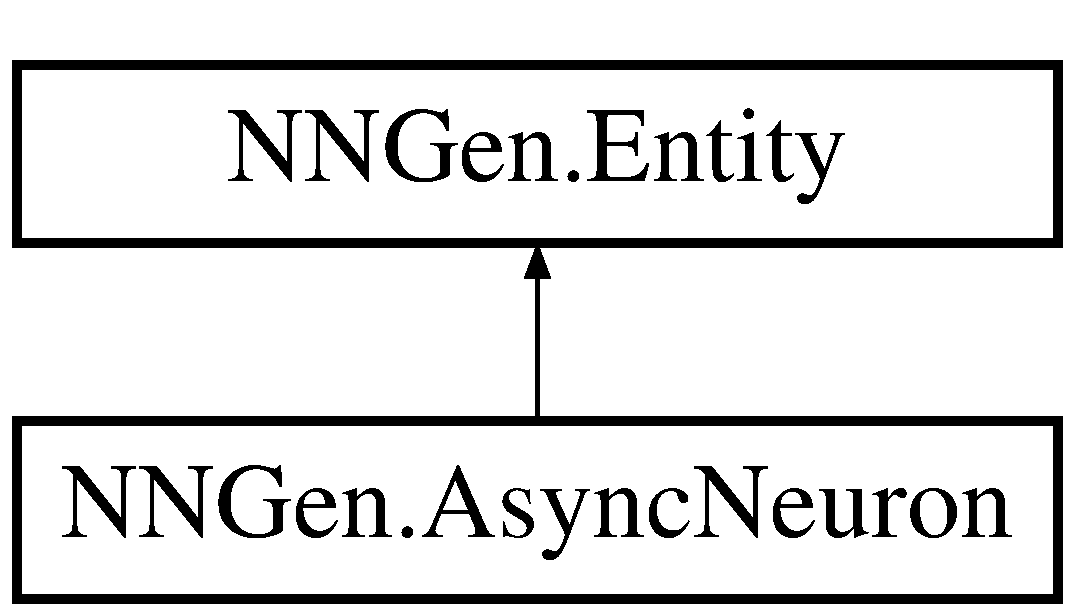
\includegraphics[height=2.000000cm]{class_n_n_gen_1_1_async_neuron}
\end{center}
\end{figure}
\subsection*{Public Types}
\begin{DoxyCompactItemize}
\item 
enum \hyperlink{class_n_n_gen_1_1_async_neuron_afe8460a52808d1587cbcc0a8e4e23b64}{Neuron\+Activation\+Type} \{ \hyperlink{class_n_n_gen_1_1_async_neuron_afe8460a52808d1587cbcc0a8e4e23b64aaac544aacc3615aada24897a215f5046}{Neuron\+Activation\+Type.\+L\+I\+N\+E\+A\+R}, 
\hyperlink{class_n_n_gen_1_1_async_neuron_afe8460a52808d1587cbcc0a8e4e23b64a71a8e1c2711781820e9e3ce31dadfd9b}{Neuron\+Activation\+Type.\+S\+I\+G\+M\+O\+I\+D\+\_\+\+P\+O\+L\+Y\+\_\+\+A\+P\+P\+R\+O\+X}, 
\hyperlink{class_n_n_gen_1_1_async_neuron_afe8460a52808d1587cbcc0a8e4e23b64ab50339a10e1de285ac99d4c3990b8693}{Neuron\+Activation\+Type.\+N\+O\+N\+E}
 \}\begin{DoxyCompactList}\small\item\em An enumeration representing the different output activation functions supported by the neuron \end{DoxyCompactList}
\end{DoxyCompactItemize}
\subsection*{Public Member Functions}
\begin{DoxyCompactItemize}
\item 
\hyperlink{class_n_n_gen_1_1_async_neuron_a38668566c40b9e34ce3f36b692fbb1ea}{Async\+Neuron} (\hyperlink{class_n_n_gen_1_1_port}{Port}\mbox{[}$\,$\mbox{]} \+\_\+input\+Ports, int \+\_\+num\+Output\+Int\+Bits, int \+\_\+num\+Output\+Frac\+Bits, int \+\_\+num\+Weight\+Int\+Bits, \hyperlink{class_n_n_gen_1_1_async_neuron_afe8460a52808d1587cbcc0a8e4e23b64}{Neuron\+Activation\+Type} \+\_\+activation\+Type, string \+\_\+name)
\begin{DoxyCompactList}\small\item\em The neuron constructor \end{DoxyCompactList}\item 
override string \hyperlink{class_n_n_gen_1_1_async_neuron_a28513dfbc9af1012436c00d02322c278}{get\+Name} ()
\begin{DoxyCompactList}\small\item\em Returns the name of the neuron \end{DoxyCompactList}\item 
override \hyperlink{class_n_n_gen_1_1_port}{Port}\mbox{[}$\,$\mbox{]} \hyperlink{class_n_n_gen_1_1_async_neuron_a76ace6a3638e3f47135fd010ebfee4a0}{get\+Input\+Ports} ()
\begin{DoxyCompactList}\small\item\em Returns the input ports to the neuron \end{DoxyCompactList}\item 
override \hyperlink{class_n_n_gen_1_1_port}{Port}\mbox{[}$\,$\mbox{]} \hyperlink{class_n_n_gen_1_1_async_neuron_ad10df3705cc6c39aaec226b0730a687e}{get\+Output\+Ports} ()
\begin{DoxyCompactList}\small\item\em Returns the output ports of the neuron \end{DoxyCompactList}\item 
override \hyperlink{class_n_n_gen_1_1_signal}{Signal}\mbox{[}$\,$\mbox{]} \hyperlink{class_n_n_gen_1_1_async_neuron_aeb97d091f87eae66eeb865557d674b72}{get\+Internal\+Signals} ()
\begin{DoxyCompactList}\small\item\em Returns a list of internal signals for the neuron \end{DoxyCompactList}\item 
override bool \hyperlink{class_n_n_gen_1_1_async_neuron_a8877af523d2fb9a4e55e74d17eb0d081}{write\+V\+H\+D\+L} (string file)
\begin{DoxyCompactList}\small\item\em Writes the .vhd file that describes the neuron. \end{DoxyCompactList}\item 
override bool \hyperlink{class_n_n_gen_1_1_async_neuron_ac096c73ce466fa58932a14ad68d0648b}{Equals} (object obj)
\begin{DoxyCompactList}\small\item\em Determines if two neurons are equal \end{DoxyCompactList}\item 
override int \hyperlink{class_n_n_gen_1_1_async_neuron_a4cc474f3e3bd5d36fbd47a6aa8b8c68f}{Get\+Hash\+Code} ()
\begin{DoxyCompactList}\small\item\em Returns the hash code of the object \end{DoxyCompactList}\end{DoxyCompactItemize}
\subsection*{Properties}
\begin{DoxyCompactItemize}
\item 
\hyperlink{class_n_n_gen_1_1_port}{Port}\mbox{[}$\,$\mbox{]} \hyperlink{class_n_n_gen_1_1_async_neuron_ae248edac3250fffe3fdba7ff2dd8288b}{neuron\+Inputs}\hspace{0.3cm}{\ttfamily  \mbox{[}get\mbox{]}}
\begin{DoxyCompactList}\small\item\em The inputs to the neuron \end{DoxyCompactList}\item 
\hyperlink{class_n_n_gen_1_1_port}{Port} \hyperlink{class_n_n_gen_1_1_async_neuron_a374b98dccdbd95b77e6e64d896220a8b}{load\+Clk\+Port}\hspace{0.3cm}{\ttfamily  \mbox{[}get\mbox{]}}
\begin{DoxyCompactList}\small\item\em A clock port used for the synchornous loading of the neuron weights \end{DoxyCompactList}\item 
\hyperlink{class_n_n_gen_1_1_port}{Port} \hyperlink{class_n_n_gen_1_1_async_neuron_a83a3e6466b062e49a29ce46508e2bdf0}{load\+Enable\+Port}\hspace{0.3cm}{\ttfamily  \mbox{[}get\mbox{]}}
\begin{DoxyCompactList}\small\item\em When high, the loading process will be enabled. \end{DoxyCompactList}\item 
\hyperlink{class_n_n_gen_1_1_port}{Port} \hyperlink{class_n_n_gen_1_1_async_neuron_a765bcf8344758b0e967117390749882d}{load\+Value\+Port}\hspace{0.3cm}{\ttfamily  \mbox{[}get\mbox{]}}
\begin{DoxyCompactList}\small\item\em During weight loading, the value presented on this port will be clocked into one of the weight signals on the rising edge of load\+Clk\+Port \end{DoxyCompactList}\item 
\hyperlink{class_n_n_gen_1_1_port}{Port} \hyperlink{class_n_n_gen_1_1_async_neuron_a96074bc794e643df031319b43efb986c}{load\+Offset\+Port}\hspace{0.3cm}{\ttfamily  \mbox{[}get\mbox{]}}
\begin{DoxyCompactList}\small\item\em During weight loading, the weight signal pointed to by this signal will be loaded with the value of load\+Value\+Port \end{DoxyCompactList}\item 
\hyperlink{class_n_n_gen_1_1_port}{Port} \hyperlink{class_n_n_gen_1_1_async_neuron_a06f594e2b75be48f0444010a2204d7b2}{final\+Load\+Port}\hspace{0.3cm}{\ttfamily  \mbox{[}get\mbox{]}}
\begin{DoxyCompactList}\small\item\em This port goes high once the final weight has been loaded \end{DoxyCompactList}\item 
\hyperlink{class_n_n_gen_1_1_port}{Port} \hyperlink{class_n_n_gen_1_1_async_neuron_a5b2ce64b48dcdfeddd29ea02a933f119}{neuron\+Output}\hspace{0.3cm}{\ttfamily  \mbox{[}get\mbox{]}}
\begin{DoxyCompactList}\small\item\em The output port from the neuron \end{DoxyCompactList}\item 
\hyperlink{class_n_n_gen_1_1_signal}{Signal}\mbox{[}$\,$\mbox{]} \hyperlink{class_n_n_gen_1_1_async_neuron_a73d47ce9be628ff13a518e071f695096}{product\+Signals}\hspace{0.3cm}{\ttfamily  \mbox{[}get\mbox{]}}
\begin{DoxyCompactList}\small\item\em The signals used for holding the value of the product (weight\+\_\+i $\ast$ input\+\_\+i) \end{DoxyCompactList}\item 
\hyperlink{class_n_n_gen_1_1_signal}{Signal}\mbox{[}$\,$\mbox{]} \hyperlink{class_n_n_gen_1_1_async_neuron_aeeb431fe55c9cda6e2889691c27c344c}{weight\+Signals}\hspace{0.3cm}{\ttfamily  \mbox{[}get\mbox{]}}
\begin{DoxyCompactList}\small\item\em The signals used for holding the weights of the network \end{DoxyCompactList}\item 
\hyperlink{class_n_n_gen_1_1_signal}{Signal} \hyperlink{class_n_n_gen_1_1_async_neuron_abcb9157df57ac1f3751b2e730703bd58}{sum}\hspace{0.3cm}{\ttfamily  \mbox{[}get\mbox{]}}
\begin{DoxyCompactList}\small\item\em The signal used for holding the value of sum(product\+\_\+i) \end{DoxyCompactList}\item 
\hyperlink{class_n_n_gen_1_1_signal}{Signal} \hyperlink{class_n_n_gen_1_1_async_neuron_a1e0f902ec842b3b970e18c4d02401c4e}{thresholded\+Sum}\hspace{0.3cm}{\ttfamily  \mbox{[}get\mbox{]}}
\begin{DoxyCompactList}\small\item\em The signal used for holding the output of the thresholding function \end{DoxyCompactList}\item 
int \hyperlink{class_n_n_gen_1_1_async_neuron_a3b0880328253a0c90da2d8ed655941bd}{num\+Output\+Frac\+Bits}\hspace{0.3cm}{\ttfamily  \mbox{[}get\mbox{]}}
\begin{DoxyCompactList}\small\item\em The number of fractional bits to maintain on the output of the neuron \end{DoxyCompactList}\item 
int \hyperlink{class_n_n_gen_1_1_async_neuron_a0a5f5459d5bfe73ec3c6e1fd584ea126}{num\+Output\+Int\+Bits}\hspace{0.3cm}{\ttfamily  \mbox{[}get\mbox{]}}
\begin{DoxyCompactList}\small\item\em The number of integer bits to maintain on the output of the neuron \end{DoxyCompactList}\item 
\hyperlink{class_n_n_gen_1_1_async_neuron_afe8460a52808d1587cbcc0a8e4e23b64}{Neuron\+Activation\+Type} \hyperlink{class_n_n_gen_1_1_async_neuron_aafa1d92f75c77c36546567c214840818}{activation\+Type}\hspace{0.3cm}{\ttfamily  \mbox{[}get\mbox{]}}
\begin{DoxyCompactList}\small\item\em The thresholding function used for the neuron \end{DoxyCompactList}\item 
string \hyperlink{class_n_n_gen_1_1_async_neuron_a1b216c193a13ad763fee071d3238aab1}{name}\hspace{0.3cm}{\ttfamily  \mbox{[}get\mbox{]}}
\begin{DoxyCompactList}\small\item\em The name of this particular neuron \end{DoxyCompactList}\end{DoxyCompactItemize}


\subsection{Detailed Description}
An abstraction of a single neuron within a network 



\subsection{Member Enumeration Documentation}
\hypertarget{class_n_n_gen_1_1_async_neuron_afe8460a52808d1587cbcc0a8e4e23b64}{}\index{N\+N\+Gen\+::\+Async\+Neuron@{N\+N\+Gen\+::\+Async\+Neuron}!Neuron\+Activation\+Type@{Neuron\+Activation\+Type}}
\index{Neuron\+Activation\+Type@{Neuron\+Activation\+Type}!N\+N\+Gen\+::\+Async\+Neuron@{N\+N\+Gen\+::\+Async\+Neuron}}
\subsubsection[{Neuron\+Activation\+Type}]{\setlength{\rightskip}{0pt plus 5cm}enum {\bf N\+N\+Gen.\+Async\+Neuron.\+Neuron\+Activation\+Type}\hspace{0.3cm}{\ttfamily [strong]}}\label{class_n_n_gen_1_1_async_neuron_afe8460a52808d1587cbcc0a8e4e23b64}


An enumeration representing the different output activation functions supported by the neuron 

\begin{Desc}
\item[Enumerator]\par
\begin{description}
\index{L\+I\+N\+E\+A\+R@{L\+I\+N\+E\+A\+R}!N\+N\+Gen\+::\+Async\+Neuron@{N\+N\+Gen\+::\+Async\+Neuron}}\index{N\+N\+Gen\+::\+Async\+Neuron@{N\+N\+Gen\+::\+Async\+Neuron}!L\+I\+N\+E\+A\+R@{L\+I\+N\+E\+A\+R}}\item[{\em 
\hypertarget{class_n_n_gen_1_1_async_neuron_afe8460a52808d1587cbcc0a8e4e23b64aaac544aacc3615aada24897a215f5046}{}L\+I\+N\+E\+A\+R\label{class_n_n_gen_1_1_async_neuron_afe8460a52808d1587cbcc0a8e4e23b64aaac544aacc3615aada24897a215f5046}
}]A linear neuron \index{S\+I\+G\+M\+O\+I\+D\+\_\+\+P\+O\+L\+Y\+\_\+\+A\+P\+P\+R\+O\+X@{S\+I\+G\+M\+O\+I\+D\+\_\+\+P\+O\+L\+Y\+\_\+\+A\+P\+P\+R\+O\+X}!N\+N\+Gen\+::\+Async\+Neuron@{N\+N\+Gen\+::\+Async\+Neuron}}\index{N\+N\+Gen\+::\+Async\+Neuron@{N\+N\+Gen\+::\+Async\+Neuron}!S\+I\+G\+M\+O\+I\+D\+\_\+\+P\+O\+L\+Y\+\_\+\+A\+P\+P\+R\+O\+X@{S\+I\+G\+M\+O\+I\+D\+\_\+\+P\+O\+L\+Y\+\_\+\+A\+P\+P\+R\+O\+X}}\item[{\em 
\hypertarget{class_n_n_gen_1_1_async_neuron_afe8460a52808d1587cbcc0a8e4e23b64a71a8e1c2711781820e9e3ce31dadfd9b}{}S\+I\+G\+M\+O\+I\+D\+\_\+\+P\+O\+L\+Y\+\_\+\+A\+P\+P\+R\+O\+X\label{class_n_n_gen_1_1_async_neuron_afe8460a52808d1587cbcc0a8e4e23b64a71a8e1c2711781820e9e3ce31dadfd9b}
}]A sigmoid approximation using f(x) $\sim$ (1/2)$\ast$(1 + (x/(x+1)) ) \index{N\+O\+N\+E@{N\+O\+N\+E}!N\+N\+Gen\+::\+Async\+Neuron@{N\+N\+Gen\+::\+Async\+Neuron}}\index{N\+N\+Gen\+::\+Async\+Neuron@{N\+N\+Gen\+::\+Async\+Neuron}!N\+O\+N\+E@{N\+O\+N\+E}}\item[{\em 
\hypertarget{class_n_n_gen_1_1_async_neuron_afe8460a52808d1587cbcc0a8e4e23b64ab50339a10e1de285ac99d4c3990b8693}{}N\+O\+N\+E\label{class_n_n_gen_1_1_async_neuron_afe8460a52808d1587cbcc0a8e4e23b64ab50339a10e1de285ac99d4c3990b8693}
}]Represents no activation function, used for input neurons \end{description}
\end{Desc}


\subsection{Constructor \& Destructor Documentation}
\hypertarget{class_n_n_gen_1_1_async_neuron_a38668566c40b9e34ce3f36b692fbb1ea}{}\index{N\+N\+Gen\+::\+Async\+Neuron@{N\+N\+Gen\+::\+Async\+Neuron}!Async\+Neuron@{Async\+Neuron}}
\index{Async\+Neuron@{Async\+Neuron}!N\+N\+Gen\+::\+Async\+Neuron@{N\+N\+Gen\+::\+Async\+Neuron}}
\subsubsection[{Async\+Neuron(\+Port[] \+\_\+input\+Ports, int \+\_\+num\+Output\+Int\+Bits, int \+\_\+num\+Output\+Frac\+Bits, int \+\_\+num\+Weight\+Int\+Bits, Neuron\+Activation\+Type \+\_\+activation\+Type, string \+\_\+name)}]{\setlength{\rightskip}{0pt plus 5cm}N\+N\+Gen.\+Async\+Neuron.\+Async\+Neuron (
\begin{DoxyParamCaption}
\item[{{\bf Port}\mbox{[}$\,$\mbox{]}}]{\+\_\+input\+Ports, }
\item[{int}]{\+\_\+num\+Output\+Int\+Bits, }
\item[{int}]{\+\_\+num\+Output\+Frac\+Bits, }
\item[{int}]{\+\_\+num\+Weight\+Int\+Bits, }
\item[{{\bf Neuron\+Activation\+Type}}]{\+\_\+activation\+Type, }
\item[{string}]{\+\_\+name}
\end{DoxyParamCaption}
)\hspace{0.3cm}{\ttfamily [inline]}}\label{class_n_n_gen_1_1_async_neuron_a38668566c40b9e34ce3f36b692fbb1ea}


The neuron constructor 


\begin{DoxyParams}{Parameters}
{\em \+\_\+input\+Ports} & An array of input ports to the neuron\\
\hline
{\em \+\_\+num\+Output\+Int\+Bits} & The number of integer bits to use on the output\\
\hline
{\em \+\_\+num\+Output\+Frac\+Bits} & The number of fractional bits to be used on the output\\
\hline
{\em \+\_\+num\+Weight\+Int\+Bits} & The number of integer bits used to represent the weights\\
\hline
{\em \+\_\+activation\+Type} & The thresholding function used to compute the output of the neuron\\
\hline
{\em \+\_\+name} & The name of the neuron\\
\hline
\end{DoxyParams}


\subsection{Member Function Documentation}
\hypertarget{class_n_n_gen_1_1_async_neuron_ac096c73ce466fa58932a14ad68d0648b}{}\index{N\+N\+Gen\+::\+Async\+Neuron@{N\+N\+Gen\+::\+Async\+Neuron}!Equals@{Equals}}
\index{Equals@{Equals}!N\+N\+Gen\+::\+Async\+Neuron@{N\+N\+Gen\+::\+Async\+Neuron}}
\subsubsection[{Equals(object obj)}]{\setlength{\rightskip}{0pt plus 5cm}override bool N\+N\+Gen.\+Async\+Neuron.\+Equals (
\begin{DoxyParamCaption}
\item[{object}]{obj}
\end{DoxyParamCaption}
)\hspace{0.3cm}{\ttfamily [inline]}}\label{class_n_n_gen_1_1_async_neuron_ac096c73ce466fa58932a14ad68d0648b}


Determines if two neurons are equal 


\begin{DoxyParams}{Parameters}
{\em obj} & Object to compare to this neuron\\
\hline
\end{DoxyParams}
\begin{DoxyReturn}{Returns}
True if the objects are equal, false otherwise
\end{DoxyReturn}
\hypertarget{class_n_n_gen_1_1_async_neuron_a4cc474f3e3bd5d36fbd47a6aa8b8c68f}{}\index{N\+N\+Gen\+::\+Async\+Neuron@{N\+N\+Gen\+::\+Async\+Neuron}!Get\+Hash\+Code@{Get\+Hash\+Code}}
\index{Get\+Hash\+Code@{Get\+Hash\+Code}!N\+N\+Gen\+::\+Async\+Neuron@{N\+N\+Gen\+::\+Async\+Neuron}}
\subsubsection[{Get\+Hash\+Code()}]{\setlength{\rightskip}{0pt plus 5cm}override int N\+N\+Gen.\+Async\+Neuron.\+Get\+Hash\+Code (
\begin{DoxyParamCaption}
{}
\end{DoxyParamCaption}
)\hspace{0.3cm}{\ttfamily [inline]}}\label{class_n_n_gen_1_1_async_neuron_a4cc474f3e3bd5d36fbd47a6aa8b8c68f}


Returns the hash code of the object 

\begin{DoxyReturn}{Returns}
The hash code of the object
\end{DoxyReturn}
\hypertarget{class_n_n_gen_1_1_async_neuron_a76ace6a3638e3f47135fd010ebfee4a0}{}\index{N\+N\+Gen\+::\+Async\+Neuron@{N\+N\+Gen\+::\+Async\+Neuron}!get\+Input\+Ports@{get\+Input\+Ports}}
\index{get\+Input\+Ports@{get\+Input\+Ports}!N\+N\+Gen\+::\+Async\+Neuron@{N\+N\+Gen\+::\+Async\+Neuron}}
\subsubsection[{get\+Input\+Ports()}]{\setlength{\rightskip}{0pt plus 5cm}override {\bf Port} \mbox{[}$\,$\mbox{]} N\+N\+Gen.\+Async\+Neuron.\+get\+Input\+Ports (
\begin{DoxyParamCaption}
{}
\end{DoxyParamCaption}
)\hspace{0.3cm}{\ttfamily [inline]}, {\ttfamily [virtual]}}\label{class_n_n_gen_1_1_async_neuron_a76ace6a3638e3f47135fd010ebfee4a0}


Returns the input ports to the neuron 

\begin{DoxyReturn}{Returns}
The input ports to the neuron
\end{DoxyReturn}


Implements \hyperlink{class_n_n_gen_1_1_entity_a01239f05c9efa61ec9e6a29cb2eaad50}{N\+N\+Gen.\+Entity}.

\hypertarget{class_n_n_gen_1_1_async_neuron_aeb97d091f87eae66eeb865557d674b72}{}\index{N\+N\+Gen\+::\+Async\+Neuron@{N\+N\+Gen\+::\+Async\+Neuron}!get\+Internal\+Signals@{get\+Internal\+Signals}}
\index{get\+Internal\+Signals@{get\+Internal\+Signals}!N\+N\+Gen\+::\+Async\+Neuron@{N\+N\+Gen\+::\+Async\+Neuron}}
\subsubsection[{get\+Internal\+Signals()}]{\setlength{\rightskip}{0pt plus 5cm}override {\bf Signal} \mbox{[}$\,$\mbox{]} N\+N\+Gen.\+Async\+Neuron.\+get\+Internal\+Signals (
\begin{DoxyParamCaption}
{}
\end{DoxyParamCaption}
)\hspace{0.3cm}{\ttfamily [inline]}, {\ttfamily [virtual]}}\label{class_n_n_gen_1_1_async_neuron_aeb97d091f87eae66eeb865557d674b72}


Returns a list of internal signals for the neuron 

\begin{DoxyReturn}{Returns}
The internal signals for the neuron
\end{DoxyReturn}


Implements \hyperlink{class_n_n_gen_1_1_entity_a62feb80e95ec84c650ea17bd53f0d510}{N\+N\+Gen.\+Entity}.

\hypertarget{class_n_n_gen_1_1_async_neuron_a28513dfbc9af1012436c00d02322c278}{}\index{N\+N\+Gen\+::\+Async\+Neuron@{N\+N\+Gen\+::\+Async\+Neuron}!get\+Name@{get\+Name}}
\index{get\+Name@{get\+Name}!N\+N\+Gen\+::\+Async\+Neuron@{N\+N\+Gen\+::\+Async\+Neuron}}
\subsubsection[{get\+Name()}]{\setlength{\rightskip}{0pt plus 5cm}override string N\+N\+Gen.\+Async\+Neuron.\+get\+Name (
\begin{DoxyParamCaption}
{}
\end{DoxyParamCaption}
)\hspace{0.3cm}{\ttfamily [inline]}, {\ttfamily [virtual]}}\label{class_n_n_gen_1_1_async_neuron_a28513dfbc9af1012436c00d02322c278}


Returns the name of the neuron 

\begin{DoxyReturn}{Returns}
The name of the neuron
\end{DoxyReturn}


Implements \hyperlink{class_n_n_gen_1_1_entity_a9f25d1070c9ab8ad343c28443e62e6f2}{N\+N\+Gen.\+Entity}.

\hypertarget{class_n_n_gen_1_1_async_neuron_ad10df3705cc6c39aaec226b0730a687e}{}\index{N\+N\+Gen\+::\+Async\+Neuron@{N\+N\+Gen\+::\+Async\+Neuron}!get\+Output\+Ports@{get\+Output\+Ports}}
\index{get\+Output\+Ports@{get\+Output\+Ports}!N\+N\+Gen\+::\+Async\+Neuron@{N\+N\+Gen\+::\+Async\+Neuron}}
\subsubsection[{get\+Output\+Ports()}]{\setlength{\rightskip}{0pt plus 5cm}override {\bf Port} \mbox{[}$\,$\mbox{]} N\+N\+Gen.\+Async\+Neuron.\+get\+Output\+Ports (
\begin{DoxyParamCaption}
{}
\end{DoxyParamCaption}
)\hspace{0.3cm}{\ttfamily [inline]}, {\ttfamily [virtual]}}\label{class_n_n_gen_1_1_async_neuron_ad10df3705cc6c39aaec226b0730a687e}


Returns the output ports of the neuron 

\begin{DoxyReturn}{Returns}
The output ports of the neuron
\end{DoxyReturn}


Implements \hyperlink{class_n_n_gen_1_1_entity_ace06368087778e254a5048c7d28747be}{N\+N\+Gen.\+Entity}.

\hypertarget{class_n_n_gen_1_1_async_neuron_a8877af523d2fb9a4e55e74d17eb0d081}{}\index{N\+N\+Gen\+::\+Async\+Neuron@{N\+N\+Gen\+::\+Async\+Neuron}!write\+V\+H\+D\+L@{write\+V\+H\+D\+L}}
\index{write\+V\+H\+D\+L@{write\+V\+H\+D\+L}!N\+N\+Gen\+::\+Async\+Neuron@{N\+N\+Gen\+::\+Async\+Neuron}}
\subsubsection[{write\+V\+H\+D\+L(string file)}]{\setlength{\rightskip}{0pt plus 5cm}override bool N\+N\+Gen.\+Async\+Neuron.\+write\+V\+H\+D\+L (
\begin{DoxyParamCaption}
\item[{string}]{file}
\end{DoxyParamCaption}
)\hspace{0.3cm}{\ttfamily [inline]}, {\ttfamily [virtual]}}\label{class_n_n_gen_1_1_async_neuron_a8877af523d2fb9a4e55e74d17eb0d081}


Writes the .vhd file that describes the neuron. 


\begin{DoxyParams}{Parameters}
{\em file} & The root file path for the network. Do not include \char`\"{}(name).\+vhd\char`\"{} in the filepath\\
\hline
\end{DoxyParams}
\begin{DoxyReturn}{Returns}
True if the file was written successfully, false otherwise
\end{DoxyReturn}


Implements \hyperlink{class_n_n_gen_1_1_entity_a1111d498446be08b20583b9625893a52}{N\+N\+Gen.\+Entity}.



\subsection{Property Documentation}
\hypertarget{class_n_n_gen_1_1_async_neuron_aafa1d92f75c77c36546567c214840818}{}\index{N\+N\+Gen\+::\+Async\+Neuron@{N\+N\+Gen\+::\+Async\+Neuron}!activation\+Type@{activation\+Type}}
\index{activation\+Type@{activation\+Type}!N\+N\+Gen\+::\+Async\+Neuron@{N\+N\+Gen\+::\+Async\+Neuron}}
\subsubsection[{activation\+Type}]{\setlength{\rightskip}{0pt plus 5cm}{\bf Neuron\+Activation\+Type} N\+N\+Gen.\+Async\+Neuron.\+activation\+Type\hspace{0.3cm}{\ttfamily [get]}}\label{class_n_n_gen_1_1_async_neuron_aafa1d92f75c77c36546567c214840818}


The thresholding function used for the neuron 

\hypertarget{class_n_n_gen_1_1_async_neuron_a06f594e2b75be48f0444010a2204d7b2}{}\index{N\+N\+Gen\+::\+Async\+Neuron@{N\+N\+Gen\+::\+Async\+Neuron}!final\+Load\+Port@{final\+Load\+Port}}
\index{final\+Load\+Port@{final\+Load\+Port}!N\+N\+Gen\+::\+Async\+Neuron@{N\+N\+Gen\+::\+Async\+Neuron}}
\subsubsection[{final\+Load\+Port}]{\setlength{\rightskip}{0pt plus 5cm}{\bf Port} N\+N\+Gen.\+Async\+Neuron.\+final\+Load\+Port\hspace{0.3cm}{\ttfamily [get]}}\label{class_n_n_gen_1_1_async_neuron_a06f594e2b75be48f0444010a2204d7b2}


This port goes high once the final weight has been loaded 

\hypertarget{class_n_n_gen_1_1_async_neuron_a374b98dccdbd95b77e6e64d896220a8b}{}\index{N\+N\+Gen\+::\+Async\+Neuron@{N\+N\+Gen\+::\+Async\+Neuron}!load\+Clk\+Port@{load\+Clk\+Port}}
\index{load\+Clk\+Port@{load\+Clk\+Port}!N\+N\+Gen\+::\+Async\+Neuron@{N\+N\+Gen\+::\+Async\+Neuron}}
\subsubsection[{load\+Clk\+Port}]{\setlength{\rightskip}{0pt plus 5cm}{\bf Port} N\+N\+Gen.\+Async\+Neuron.\+load\+Clk\+Port\hspace{0.3cm}{\ttfamily [get]}}\label{class_n_n_gen_1_1_async_neuron_a374b98dccdbd95b77e6e64d896220a8b}


A clock port used for the synchornous loading of the neuron weights 

\hypertarget{class_n_n_gen_1_1_async_neuron_a83a3e6466b062e49a29ce46508e2bdf0}{}\index{N\+N\+Gen\+::\+Async\+Neuron@{N\+N\+Gen\+::\+Async\+Neuron}!load\+Enable\+Port@{load\+Enable\+Port}}
\index{load\+Enable\+Port@{load\+Enable\+Port}!N\+N\+Gen\+::\+Async\+Neuron@{N\+N\+Gen\+::\+Async\+Neuron}}
\subsubsection[{load\+Enable\+Port}]{\setlength{\rightskip}{0pt plus 5cm}{\bf Port} N\+N\+Gen.\+Async\+Neuron.\+load\+Enable\+Port\hspace{0.3cm}{\ttfamily [get]}}\label{class_n_n_gen_1_1_async_neuron_a83a3e6466b062e49a29ce46508e2bdf0}


When high, the loading process will be enabled. 

\hypertarget{class_n_n_gen_1_1_async_neuron_a96074bc794e643df031319b43efb986c}{}\index{N\+N\+Gen\+::\+Async\+Neuron@{N\+N\+Gen\+::\+Async\+Neuron}!load\+Offset\+Port@{load\+Offset\+Port}}
\index{load\+Offset\+Port@{load\+Offset\+Port}!N\+N\+Gen\+::\+Async\+Neuron@{N\+N\+Gen\+::\+Async\+Neuron}}
\subsubsection[{load\+Offset\+Port}]{\setlength{\rightskip}{0pt plus 5cm}{\bf Port} N\+N\+Gen.\+Async\+Neuron.\+load\+Offset\+Port\hspace{0.3cm}{\ttfamily [get]}}\label{class_n_n_gen_1_1_async_neuron_a96074bc794e643df031319b43efb986c}


During weight loading, the weight signal pointed to by this signal will be loaded with the value of load\+Value\+Port 

\hypertarget{class_n_n_gen_1_1_async_neuron_a765bcf8344758b0e967117390749882d}{}\index{N\+N\+Gen\+::\+Async\+Neuron@{N\+N\+Gen\+::\+Async\+Neuron}!load\+Value\+Port@{load\+Value\+Port}}
\index{load\+Value\+Port@{load\+Value\+Port}!N\+N\+Gen\+::\+Async\+Neuron@{N\+N\+Gen\+::\+Async\+Neuron}}
\subsubsection[{load\+Value\+Port}]{\setlength{\rightskip}{0pt plus 5cm}{\bf Port} N\+N\+Gen.\+Async\+Neuron.\+load\+Value\+Port\hspace{0.3cm}{\ttfamily [get]}}\label{class_n_n_gen_1_1_async_neuron_a765bcf8344758b0e967117390749882d}


During weight loading, the value presented on this port will be clocked into one of the weight signals on the rising edge of load\+Clk\+Port 

\hypertarget{class_n_n_gen_1_1_async_neuron_a1b216c193a13ad763fee071d3238aab1}{}\index{N\+N\+Gen\+::\+Async\+Neuron@{N\+N\+Gen\+::\+Async\+Neuron}!name@{name}}
\index{name@{name}!N\+N\+Gen\+::\+Async\+Neuron@{N\+N\+Gen\+::\+Async\+Neuron}}
\subsubsection[{name}]{\setlength{\rightskip}{0pt plus 5cm}string N\+N\+Gen.\+Async\+Neuron.\+name\hspace{0.3cm}{\ttfamily [get]}}\label{class_n_n_gen_1_1_async_neuron_a1b216c193a13ad763fee071d3238aab1}


The name of this particular neuron 

\hypertarget{class_n_n_gen_1_1_async_neuron_ae248edac3250fffe3fdba7ff2dd8288b}{}\index{N\+N\+Gen\+::\+Async\+Neuron@{N\+N\+Gen\+::\+Async\+Neuron}!neuron\+Inputs@{neuron\+Inputs}}
\index{neuron\+Inputs@{neuron\+Inputs}!N\+N\+Gen\+::\+Async\+Neuron@{N\+N\+Gen\+::\+Async\+Neuron}}
\subsubsection[{neuron\+Inputs}]{\setlength{\rightskip}{0pt plus 5cm}{\bf Port} \mbox{[}$\,$\mbox{]} N\+N\+Gen.\+Async\+Neuron.\+neuron\+Inputs\hspace{0.3cm}{\ttfamily [get]}}\label{class_n_n_gen_1_1_async_neuron_ae248edac3250fffe3fdba7ff2dd8288b}


The inputs to the neuron 

\hypertarget{class_n_n_gen_1_1_async_neuron_a5b2ce64b48dcdfeddd29ea02a933f119}{}\index{N\+N\+Gen\+::\+Async\+Neuron@{N\+N\+Gen\+::\+Async\+Neuron}!neuron\+Output@{neuron\+Output}}
\index{neuron\+Output@{neuron\+Output}!N\+N\+Gen\+::\+Async\+Neuron@{N\+N\+Gen\+::\+Async\+Neuron}}
\subsubsection[{neuron\+Output}]{\setlength{\rightskip}{0pt plus 5cm}{\bf Port} N\+N\+Gen.\+Async\+Neuron.\+neuron\+Output\hspace{0.3cm}{\ttfamily [get]}}\label{class_n_n_gen_1_1_async_neuron_a5b2ce64b48dcdfeddd29ea02a933f119}


The output port from the neuron 

\hypertarget{class_n_n_gen_1_1_async_neuron_a3b0880328253a0c90da2d8ed655941bd}{}\index{N\+N\+Gen\+::\+Async\+Neuron@{N\+N\+Gen\+::\+Async\+Neuron}!num\+Output\+Frac\+Bits@{num\+Output\+Frac\+Bits}}
\index{num\+Output\+Frac\+Bits@{num\+Output\+Frac\+Bits}!N\+N\+Gen\+::\+Async\+Neuron@{N\+N\+Gen\+::\+Async\+Neuron}}
\subsubsection[{num\+Output\+Frac\+Bits}]{\setlength{\rightskip}{0pt plus 5cm}int N\+N\+Gen.\+Async\+Neuron.\+num\+Output\+Frac\+Bits\hspace{0.3cm}{\ttfamily [get]}}\label{class_n_n_gen_1_1_async_neuron_a3b0880328253a0c90da2d8ed655941bd}


The number of fractional bits to maintain on the output of the neuron 

\hypertarget{class_n_n_gen_1_1_async_neuron_a0a5f5459d5bfe73ec3c6e1fd584ea126}{}\index{N\+N\+Gen\+::\+Async\+Neuron@{N\+N\+Gen\+::\+Async\+Neuron}!num\+Output\+Int\+Bits@{num\+Output\+Int\+Bits}}
\index{num\+Output\+Int\+Bits@{num\+Output\+Int\+Bits}!N\+N\+Gen\+::\+Async\+Neuron@{N\+N\+Gen\+::\+Async\+Neuron}}
\subsubsection[{num\+Output\+Int\+Bits}]{\setlength{\rightskip}{0pt plus 5cm}int N\+N\+Gen.\+Async\+Neuron.\+num\+Output\+Int\+Bits\hspace{0.3cm}{\ttfamily [get]}}\label{class_n_n_gen_1_1_async_neuron_a0a5f5459d5bfe73ec3c6e1fd584ea126}


The number of integer bits to maintain on the output of the neuron 

\hypertarget{class_n_n_gen_1_1_async_neuron_a73d47ce9be628ff13a518e071f695096}{}\index{N\+N\+Gen\+::\+Async\+Neuron@{N\+N\+Gen\+::\+Async\+Neuron}!product\+Signals@{product\+Signals}}
\index{product\+Signals@{product\+Signals}!N\+N\+Gen\+::\+Async\+Neuron@{N\+N\+Gen\+::\+Async\+Neuron}}
\subsubsection[{product\+Signals}]{\setlength{\rightskip}{0pt plus 5cm}{\bf Signal} \mbox{[}$\,$\mbox{]} N\+N\+Gen.\+Async\+Neuron.\+product\+Signals\hspace{0.3cm}{\ttfamily [get]}}\label{class_n_n_gen_1_1_async_neuron_a73d47ce9be628ff13a518e071f695096}


The signals used for holding the value of the product (weight\+\_\+i $\ast$ input\+\_\+i) 

\hypertarget{class_n_n_gen_1_1_async_neuron_abcb9157df57ac1f3751b2e730703bd58}{}\index{N\+N\+Gen\+::\+Async\+Neuron@{N\+N\+Gen\+::\+Async\+Neuron}!sum@{sum}}
\index{sum@{sum}!N\+N\+Gen\+::\+Async\+Neuron@{N\+N\+Gen\+::\+Async\+Neuron}}
\subsubsection[{sum}]{\setlength{\rightskip}{0pt plus 5cm}{\bf Signal} N\+N\+Gen.\+Async\+Neuron.\+sum\hspace{0.3cm}{\ttfamily [get]}}\label{class_n_n_gen_1_1_async_neuron_abcb9157df57ac1f3751b2e730703bd58}


The signal used for holding the value of sum(product\+\_\+i) 

\hypertarget{class_n_n_gen_1_1_async_neuron_a1e0f902ec842b3b970e18c4d02401c4e}{}\index{N\+N\+Gen\+::\+Async\+Neuron@{N\+N\+Gen\+::\+Async\+Neuron}!thresholded\+Sum@{thresholded\+Sum}}
\index{thresholded\+Sum@{thresholded\+Sum}!N\+N\+Gen\+::\+Async\+Neuron@{N\+N\+Gen\+::\+Async\+Neuron}}
\subsubsection[{thresholded\+Sum}]{\setlength{\rightskip}{0pt plus 5cm}{\bf Signal} N\+N\+Gen.\+Async\+Neuron.\+thresholded\+Sum\hspace{0.3cm}{\ttfamily [get]}}\label{class_n_n_gen_1_1_async_neuron_a1e0f902ec842b3b970e18c4d02401c4e}


The signal used for holding the output of the thresholding function 

\hypertarget{class_n_n_gen_1_1_async_neuron_aeeb431fe55c9cda6e2889691c27c344c}{}\index{N\+N\+Gen\+::\+Async\+Neuron@{N\+N\+Gen\+::\+Async\+Neuron}!weight\+Signals@{weight\+Signals}}
\index{weight\+Signals@{weight\+Signals}!N\+N\+Gen\+::\+Async\+Neuron@{N\+N\+Gen\+::\+Async\+Neuron}}
\subsubsection[{weight\+Signals}]{\setlength{\rightskip}{0pt plus 5cm}{\bf Signal} \mbox{[}$\,$\mbox{]} N\+N\+Gen.\+Async\+Neuron.\+weight\+Signals\hspace{0.3cm}{\ttfamily [get]}}\label{class_n_n_gen_1_1_async_neuron_aeeb431fe55c9cda6e2889691c27c344c}


The signals used for holding the weights of the network 



The documentation for this class was generated from the following file\+:\begin{DoxyCompactItemize}
\item 
E\+:/\+Documents/\+Visual Studio 2013/\+Projects/\+Neural\+Network/\+N\+N\+Gen/\hyperlink{_async_neuron_8cs}{Async\+Neuron.\+cs}\end{DoxyCompactItemize}

\hypertarget{class_n_n_gen_1_1_entity}{}\section{N\+N\+Gen.\+Entity Class Reference}
\label{class_n_n_gen_1_1_entity}\index{N\+N\+Gen.\+Entity@{N\+N\+Gen.\+Entity}}


An interface for any object that will eventually generate a V\+H\+D\+L entity  


Inheritance diagram for N\+N\+Gen.\+Entity\+:\begin{figure}[H]
\begin{center}
\leavevmode
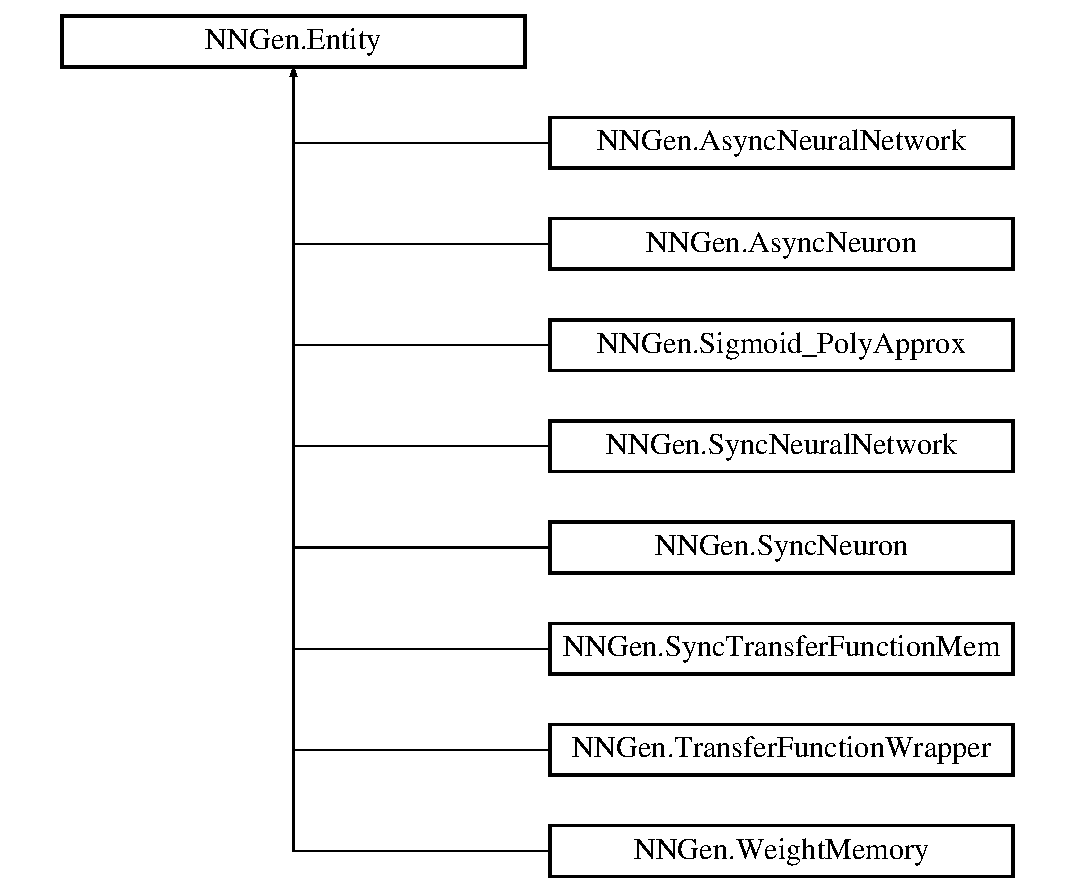
\includegraphics[height=9.000000cm]{class_n_n_gen_1_1_entity}
\end{center}
\end{figure}
\subsection*{Public Member Functions}
\begin{DoxyCompactItemize}
\item 
abstract string \hyperlink{class_n_n_gen_1_1_entity_a9f25d1070c9ab8ad343c28443e62e6f2}{get\+Name} ()
\begin{DoxyCompactList}\small\item\em Returns a string representing the name of the entity (i.\+e. the X\+X\+X in the line \char`\"{}\+E\+N\+T\+I\+T\+Y X\+X\+X I\+S ...\char`\"{}) \end{DoxyCompactList}\item 
abstract \hyperlink{class_n_n_gen_1_1_port}{Port}\mbox{[}$\,$\mbox{]} \hyperlink{class_n_n_gen_1_1_entity_a01239f05c9efa61ec9e6a29cb2eaad50}{get\+Input\+Ports} ()
\begin{DoxyCompactList}\small\item\em Returns an array of Ports representing the inputs to the entity \end{DoxyCompactList}\item 
abstract \hyperlink{class_n_n_gen_1_1_port}{Port}\mbox{[}$\,$\mbox{]} \hyperlink{class_n_n_gen_1_1_entity_ace06368087778e254a5048c7d28747be}{get\+Output\+Ports} ()
\begin{DoxyCompactList}\small\item\em Returns an array of Ports representing the outputs of the entity \end{DoxyCompactList}\item 
abstract \hyperlink{class_n_n_gen_1_1_signal}{Signal}\mbox{[}$\,$\mbox{]} \hyperlink{class_n_n_gen_1_1_entity_a62feb80e95ec84c650ea17bd53f0d510}{get\+Internal\+Signals} ()
\begin{DoxyCompactList}\small\item\em Returns an array of singnals representing the internal signals of the entity \end{DoxyCompactList}\item 
abstract bool \hyperlink{class_n_n_gen_1_1_entity_a1111d498446be08b20583b9625893a52}{write\+V\+H\+D\+L} (string file)
\begin{DoxyCompactList}\small\item\em Writes the V\+H\+D\+L entity to file. \end{DoxyCompactList}\item 
bool \hyperlink{class_n_n_gen_1_1_entity_a75a568e4f2375bb409c5f31e17bf2585}{write\+V\+H\+D\+L\+Includes} (Stream\+Writer sw)
\begin{DoxyCompactList}\small\item\em Writes the \char`\"{}library\char`\"{} and \char`\"{}use\char`\"{} include statements for the project \end{DoxyCompactList}\item 
bool \hyperlink{class_n_n_gen_1_1_entity_a9c1e22927e3bb62cbfbf391dc1c52301}{write\+V\+H\+D\+L\+Entity} (Stream\+Writer sw)
\begin{DoxyCompactList}\small\item\em Writes an entity statement "E\+N\+T\+I\+T\+Y ... I\+S P\+O\+R\+T ( ... ); E\+N\+D ...; \end{DoxyCompactList}\item 
bool \hyperlink{class_n_n_gen_1_1_entity_aee5c9d1fd7354d1b571f4d99043a0f51}{write\+V\+H\+D\+L\+Component} (Stream\+Writer sw)
\begin{DoxyCompactList}\small\item\em Writes a component statment, used to declare smaller entities within a larger entity C\+O\+M\+P\+O\+N\+E\+N\+T ... P\+O\+R\+T ( ... ); E\+N\+D C\+O\+M\+P\+O\+N\+E\+N\+T; \end{DoxyCompactList}\item 
bool \hyperlink{class_n_n_gen_1_1_entity_a9e1d15aff6a09e55419661983923e4b7}{write\+V\+H\+D\+L\+Ports} (Stream\+Writer sw)
\begin{DoxyCompactList}\small\item\em Writes the port statement for a V\+H\+D\+L entity P\+O\+R\+T ( ... ); \end{DoxyCompactList}\item 
bool \hyperlink{class_n_n_gen_1_1_entity_a841b967c6c90e24c6d5fe9ad2a420751}{write\+V\+H\+D\+L\+Dependencies} (Stream\+Writer sw, List$<$ \hyperlink{class_n_n_gen_1_1_entity}{Entity} $>$ dependent\+Entities)
\begin{DoxyCompactList}\small\item\em Writes the component statment for each of the entities in dependent\+Entities See \hyperlink{class_n_n_gen_1_1_entity_aee5c9d1fd7354d1b571f4d99043a0f51}{write\+V\+H\+D\+L\+Component()} \end{DoxyCompactList}\item 
bool \hyperlink{class_n_n_gen_1_1_entity_afb8bc38d1bea3b52be2557c2447942ef}{write\+V\+H\+D\+L\+Signals} (Stream\+Writer sw)
\begin{DoxyCompactList}\small\item\em Writes the internal signals for the entity S\+I\+G\+N\+A\+L ... \end{DoxyCompactList}\item 
bool \hyperlink{class_n_n_gen_1_1_entity_a643e1423f3ec04732cc2dd660ff97c33}{write\+Architecture\+Statement} (Stream\+Writer sw)
\begin{DoxyCompactList}\small\item\em Writes the architecture statment for the entity A\+R\+C\+H\+I\+T\+E\+C\+T\+U\+R\+E ... O\+F ... I\+S \end{DoxyCompactList}\item 
bool \hyperlink{class_n_n_gen_1_1_entity_adfad533f41068a59a73ce65805e86081}{write\+V\+H\+D\+L\+Footer} (Stream\+Writer sw)
\begin{DoxyCompactList}\small\item\em Writes the V\+H\+D\+L footer for the entity and flushes the stream E\+N\+D A\+R\+C\+H\+I\+T\+E\+C\+T\+U\+R\+E; \end{DoxyCompactList}\end{DoxyCompactItemize}


\subsection{Detailed Description}
An interface for any object that will eventually generate a V\+H\+D\+L entity 



\subsection{Member Function Documentation}
\hypertarget{class_n_n_gen_1_1_entity_a01239f05c9efa61ec9e6a29cb2eaad50}{}\index{N\+N\+Gen\+::\+Entity@{N\+N\+Gen\+::\+Entity}!get\+Input\+Ports@{get\+Input\+Ports}}
\index{get\+Input\+Ports@{get\+Input\+Ports}!N\+N\+Gen\+::\+Entity@{N\+N\+Gen\+::\+Entity}}
\subsubsection[{get\+Input\+Ports()}]{\setlength{\rightskip}{0pt plus 5cm}abstract {\bf Port} \mbox{[}$\,$\mbox{]} N\+N\+Gen.\+Entity.\+get\+Input\+Ports (
\begin{DoxyParamCaption}
{}
\end{DoxyParamCaption}
)\hspace{0.3cm}{\ttfamily [pure virtual]}}\label{class_n_n_gen_1_1_entity_a01239f05c9efa61ec9e6a29cb2eaad50}


Returns an array of Ports representing the inputs to the entity 

\begin{DoxyReturn}{Returns}
The inputs to the entity
\end{DoxyReturn}


Implemented in \hyperlink{class_n_n_gen_1_1_async_neural_network_a94ad9532f7e80514db3ff3eb16ba42cf}{N\+N\+Gen.\+Async\+Neural\+Network}, \hyperlink{class_n_n_gen_1_1_sync_neural_network_a8ed253e22e640d3ec0501dd1c43ad784}{N\+N\+Gen.\+Sync\+Neural\+Network}, \hyperlink{class_n_n_gen_1_1_async_neuron_a76ace6a3638e3f47135fd010ebfee4a0}{N\+N\+Gen.\+Async\+Neuron}, \hyperlink{class_n_n_gen_1_1_transfer_function_wrapper_a383f86ef468440ca41a5018c8670c2ef}{N\+N\+Gen.\+Transfer\+Function\+Wrapper}, \hyperlink{class_n_n_gen_1_1_sync_neuron_a9f391d4a186cdd79f97ece5adab9ff6c}{N\+N\+Gen.\+Sync\+Neuron}, \hyperlink{class_n_n_gen_1_1_sigmoid___poly_approx_ac4cf07415c0dc69efdaf91cfc561b68f}{N\+N\+Gen.\+Sigmoid\+\_\+\+Poly\+Approx}, \hyperlink{class_n_n_gen_1_1_sync_transfer_function_mem_a4e263ba9743751277b49cd90578e2455}{N\+N\+Gen.\+Sync\+Transfer\+Function\+Mem}, and \hyperlink{class_n_n_gen_1_1_weight_memory_a0f80fe3a06082c2e238f1c7b552c723d}{N\+N\+Gen.\+Weight\+Memory}.

\hypertarget{class_n_n_gen_1_1_entity_a62feb80e95ec84c650ea17bd53f0d510}{}\index{N\+N\+Gen\+::\+Entity@{N\+N\+Gen\+::\+Entity}!get\+Internal\+Signals@{get\+Internal\+Signals}}
\index{get\+Internal\+Signals@{get\+Internal\+Signals}!N\+N\+Gen\+::\+Entity@{N\+N\+Gen\+::\+Entity}}
\subsubsection[{get\+Internal\+Signals()}]{\setlength{\rightskip}{0pt plus 5cm}abstract {\bf Signal} \mbox{[}$\,$\mbox{]} N\+N\+Gen.\+Entity.\+get\+Internal\+Signals (
\begin{DoxyParamCaption}
{}
\end{DoxyParamCaption}
)\hspace{0.3cm}{\ttfamily [pure virtual]}}\label{class_n_n_gen_1_1_entity_a62feb80e95ec84c650ea17bd53f0d510}


Returns an array of singnals representing the internal signals of the entity 

\begin{DoxyReturn}{Returns}
The internal signals of the entity
\end{DoxyReturn}


Implemented in \hyperlink{class_n_n_gen_1_1_async_neural_network_a4ef8c71674da4a162680bf5b5c22d928}{N\+N\+Gen.\+Async\+Neural\+Network}, \hyperlink{class_n_n_gen_1_1_sync_neural_network_a9303b53dc2d792c18ffa72e386eb0eae}{N\+N\+Gen.\+Sync\+Neural\+Network}, \hyperlink{class_n_n_gen_1_1_async_neuron_aeb97d091f87eae66eeb865557d674b72}{N\+N\+Gen.\+Async\+Neuron}, \hyperlink{class_n_n_gen_1_1_transfer_function_wrapper_ae64279d96fae0f113bf6cf0cfbadfdff}{N\+N\+Gen.\+Transfer\+Function\+Wrapper}, \hyperlink{class_n_n_gen_1_1_sync_neuron_a615a906839d1227ca0e4605b4165f892}{N\+N\+Gen.\+Sync\+Neuron}, \hyperlink{class_n_n_gen_1_1_sigmoid___poly_approx_aa9ea30f1d5fa7e2ff1874f00e37deffb}{N\+N\+Gen.\+Sigmoid\+\_\+\+Poly\+Approx}, \hyperlink{class_n_n_gen_1_1_sync_transfer_function_mem_a6b11efb6fd2d874b9bb5cfaafdb528a5}{N\+N\+Gen.\+Sync\+Transfer\+Function\+Mem}, and \hyperlink{class_n_n_gen_1_1_weight_memory_a7166780b7824c585e92da81172aaba22}{N\+N\+Gen.\+Weight\+Memory}.

\hypertarget{class_n_n_gen_1_1_entity_a9f25d1070c9ab8ad343c28443e62e6f2}{}\index{N\+N\+Gen\+::\+Entity@{N\+N\+Gen\+::\+Entity}!get\+Name@{get\+Name}}
\index{get\+Name@{get\+Name}!N\+N\+Gen\+::\+Entity@{N\+N\+Gen\+::\+Entity}}
\subsubsection[{get\+Name()}]{\setlength{\rightskip}{0pt plus 5cm}abstract string N\+N\+Gen.\+Entity.\+get\+Name (
\begin{DoxyParamCaption}
{}
\end{DoxyParamCaption}
)\hspace{0.3cm}{\ttfamily [pure virtual]}}\label{class_n_n_gen_1_1_entity_a9f25d1070c9ab8ad343c28443e62e6f2}


Returns a string representing the name of the entity (i.\+e. the X\+X\+X in the line \char`\"{}\+E\+N\+T\+I\+T\+Y X\+X\+X I\+S ...\char`\"{}) 

\begin{DoxyReturn}{Returns}
Name of the entity
\end{DoxyReturn}


Implemented in \hyperlink{class_n_n_gen_1_1_async_neural_network_affd3f3ffb007593e408d63dccf256238}{N\+N\+Gen.\+Async\+Neural\+Network}, \hyperlink{class_n_n_gen_1_1_sync_neural_network_a91d58e0d612c6398c3164dee0fc34347}{N\+N\+Gen.\+Sync\+Neural\+Network}, \hyperlink{class_n_n_gen_1_1_async_neuron_a28513dfbc9af1012436c00d02322c278}{N\+N\+Gen.\+Async\+Neuron}, \hyperlink{class_n_n_gen_1_1_transfer_function_wrapper_a0ee97f1271edd325188fe389f1b25372}{N\+N\+Gen.\+Transfer\+Function\+Wrapper}, \hyperlink{class_n_n_gen_1_1_sync_neuron_a0d24dc5f802b28e58318bbc70e4e999a}{N\+N\+Gen.\+Sync\+Neuron}, \hyperlink{class_n_n_gen_1_1_sigmoid___poly_approx_a68e8a0e324f6cae64ee7d2f841c35506}{N\+N\+Gen.\+Sigmoid\+\_\+\+Poly\+Approx}, \hyperlink{class_n_n_gen_1_1_sync_transfer_function_mem_ad4e64419e06ee98cd0a8e52d7ed866b6}{N\+N\+Gen.\+Sync\+Transfer\+Function\+Mem}, and \hyperlink{class_n_n_gen_1_1_weight_memory_a000cfa9b5dd1d41042ed77dbad178aeb}{N\+N\+Gen.\+Weight\+Memory}.

\hypertarget{class_n_n_gen_1_1_entity_ace06368087778e254a5048c7d28747be}{}\index{N\+N\+Gen\+::\+Entity@{N\+N\+Gen\+::\+Entity}!get\+Output\+Ports@{get\+Output\+Ports}}
\index{get\+Output\+Ports@{get\+Output\+Ports}!N\+N\+Gen\+::\+Entity@{N\+N\+Gen\+::\+Entity}}
\subsubsection[{get\+Output\+Ports()}]{\setlength{\rightskip}{0pt plus 5cm}abstract {\bf Port} \mbox{[}$\,$\mbox{]} N\+N\+Gen.\+Entity.\+get\+Output\+Ports (
\begin{DoxyParamCaption}
{}
\end{DoxyParamCaption}
)\hspace{0.3cm}{\ttfamily [pure virtual]}}\label{class_n_n_gen_1_1_entity_ace06368087778e254a5048c7d28747be}


Returns an array of Ports representing the outputs of the entity 

\begin{DoxyReturn}{Returns}
The outputs of the entity
\end{DoxyReturn}


Implemented in \hyperlink{class_n_n_gen_1_1_async_neural_network_a1efde159a323347b01cd88527d61c14e}{N\+N\+Gen.\+Async\+Neural\+Network}, \hyperlink{class_n_n_gen_1_1_sync_neural_network_aff93a78db054336cfe8b2f43885f145d}{N\+N\+Gen.\+Sync\+Neural\+Network}, \hyperlink{class_n_n_gen_1_1_async_neuron_ad10df3705cc6c39aaec226b0730a687e}{N\+N\+Gen.\+Async\+Neuron}, \hyperlink{class_n_n_gen_1_1_transfer_function_wrapper_ae687574b26429fd7853a53df4759ca90}{N\+N\+Gen.\+Transfer\+Function\+Wrapper}, \hyperlink{class_n_n_gen_1_1_sync_neuron_a79f19432c86cbaf3a2eaa2090cecf9cf}{N\+N\+Gen.\+Sync\+Neuron}, \hyperlink{class_n_n_gen_1_1_sigmoid___poly_approx_ad4add2a8c53cc31373dab81e8ea634e2}{N\+N\+Gen.\+Sigmoid\+\_\+\+Poly\+Approx}, \hyperlink{class_n_n_gen_1_1_sync_transfer_function_mem_a56548ab0fbafaa0384aa3c5cddc4d050}{N\+N\+Gen.\+Sync\+Transfer\+Function\+Mem}, and \hyperlink{class_n_n_gen_1_1_weight_memory_a96cae98991fe72526efcc94aa27c3294}{N\+N\+Gen.\+Weight\+Memory}.

\hypertarget{class_n_n_gen_1_1_entity_a643e1423f3ec04732cc2dd660ff97c33}{}\index{N\+N\+Gen\+::\+Entity@{N\+N\+Gen\+::\+Entity}!write\+Architecture\+Statement@{write\+Architecture\+Statement}}
\index{write\+Architecture\+Statement@{write\+Architecture\+Statement}!N\+N\+Gen\+::\+Entity@{N\+N\+Gen\+::\+Entity}}
\subsubsection[{write\+Architecture\+Statement(\+Stream\+Writer sw)}]{\setlength{\rightskip}{0pt plus 5cm}bool N\+N\+Gen.\+Entity.\+write\+Architecture\+Statement (
\begin{DoxyParamCaption}
\item[{Stream\+Writer}]{sw}
\end{DoxyParamCaption}
)\hspace{0.3cm}{\ttfamily [inline]}}\label{class_n_n_gen_1_1_entity_a643e1423f3ec04732cc2dd660ff97c33}


Writes the architecture statment for the entity A\+R\+C\+H\+I\+T\+E\+C\+T\+U\+R\+E ... O\+F ... I\+S 


\begin{DoxyParams}{Parameters}
{\em sw} & The stream in which to write. Must be open and valid\\
\hline
\end{DoxyParams}
\begin{DoxyReturn}{Returns}
True if the lines were written successfully, false otherwise
\end{DoxyReturn}
\hypertarget{class_n_n_gen_1_1_entity_a1111d498446be08b20583b9625893a52}{}\index{N\+N\+Gen\+::\+Entity@{N\+N\+Gen\+::\+Entity}!write\+V\+H\+D\+L@{write\+V\+H\+D\+L}}
\index{write\+V\+H\+D\+L@{write\+V\+H\+D\+L}!N\+N\+Gen\+::\+Entity@{N\+N\+Gen\+::\+Entity}}
\subsubsection[{write\+V\+H\+D\+L(string file)}]{\setlength{\rightskip}{0pt plus 5cm}abstract bool N\+N\+Gen.\+Entity.\+write\+V\+H\+D\+L (
\begin{DoxyParamCaption}
\item[{string}]{file}
\end{DoxyParamCaption}
)\hspace{0.3cm}{\ttfamily [pure virtual]}}\label{class_n_n_gen_1_1_entity_a1111d498446be08b20583b9625893a52}


Writes the V\+H\+D\+L entity to file. 


\begin{DoxyParams}{Parameters}
{\em file} & The file path to which the entity is to be written\\
\hline
\end{DoxyParams}
\begin{DoxyReturn}{Returns}
True if the file was written successfully, false otherwise.
\end{DoxyReturn}


Implemented in \hyperlink{class_n_n_gen_1_1_async_neural_network_ad57a90889256277e0da34e8e7f3e7848}{N\+N\+Gen.\+Async\+Neural\+Network}, \hyperlink{class_n_n_gen_1_1_sync_neural_network_ab236b9511b805fa1cabe60f3a2c871d6}{N\+N\+Gen.\+Sync\+Neural\+Network}, \hyperlink{class_n_n_gen_1_1_async_neuron_a8877af523d2fb9a4e55e74d17eb0d081}{N\+N\+Gen.\+Async\+Neuron}, \hyperlink{class_n_n_gen_1_1_transfer_function_wrapper_a1c011e274cd2df8fc643228d77619890}{N\+N\+Gen.\+Transfer\+Function\+Wrapper}, \hyperlink{class_n_n_gen_1_1_sync_neuron_aebc20821885a0661e98403b4a7722643}{N\+N\+Gen.\+Sync\+Neuron}, \hyperlink{class_n_n_gen_1_1_sigmoid___poly_approx_a1d78cd23e2a1f4e686980052ad8c7a44}{N\+N\+Gen.\+Sigmoid\+\_\+\+Poly\+Approx}, \hyperlink{class_n_n_gen_1_1_sync_transfer_function_mem_a6262571443276194d157c94be915f069}{N\+N\+Gen.\+Sync\+Transfer\+Function\+Mem}, and \hyperlink{class_n_n_gen_1_1_weight_memory_a638a0f1ce7d8f3983ef0a0beb59e887d}{N\+N\+Gen.\+Weight\+Memory}.

\hypertarget{class_n_n_gen_1_1_entity_aee5c9d1fd7354d1b571f4d99043a0f51}{}\index{N\+N\+Gen\+::\+Entity@{N\+N\+Gen\+::\+Entity}!write\+V\+H\+D\+L\+Component@{write\+V\+H\+D\+L\+Component}}
\index{write\+V\+H\+D\+L\+Component@{write\+V\+H\+D\+L\+Component}!N\+N\+Gen\+::\+Entity@{N\+N\+Gen\+::\+Entity}}
\subsubsection[{write\+V\+H\+D\+L\+Component(\+Stream\+Writer sw)}]{\setlength{\rightskip}{0pt plus 5cm}bool N\+N\+Gen.\+Entity.\+write\+V\+H\+D\+L\+Component (
\begin{DoxyParamCaption}
\item[{Stream\+Writer}]{sw}
\end{DoxyParamCaption}
)\hspace{0.3cm}{\ttfamily [inline]}}\label{class_n_n_gen_1_1_entity_aee5c9d1fd7354d1b571f4d99043a0f51}


Writes a component statment, used to declare smaller entities within a larger entity C\+O\+M\+P\+O\+N\+E\+N\+T ... P\+O\+R\+T ( ... ); E\+N\+D C\+O\+M\+P\+O\+N\+E\+N\+T; 


\begin{DoxyParams}{Parameters}
{\em sw} & The stream in which to write. Must be open and valid\\
\hline
\end{DoxyParams}
\begin{DoxyReturn}{Returns}
True if the lines were written successfully, false otherwise
\end{DoxyReturn}
\hypertarget{class_n_n_gen_1_1_entity_a841b967c6c90e24c6d5fe9ad2a420751}{}\index{N\+N\+Gen\+::\+Entity@{N\+N\+Gen\+::\+Entity}!write\+V\+H\+D\+L\+Dependencies@{write\+V\+H\+D\+L\+Dependencies}}
\index{write\+V\+H\+D\+L\+Dependencies@{write\+V\+H\+D\+L\+Dependencies}!N\+N\+Gen\+::\+Entity@{N\+N\+Gen\+::\+Entity}}
\subsubsection[{write\+V\+H\+D\+L\+Dependencies(\+Stream\+Writer sw, List$<$ Entity $>$ dependent\+Entities)}]{\setlength{\rightskip}{0pt plus 5cm}bool N\+N\+Gen.\+Entity.\+write\+V\+H\+D\+L\+Dependencies (
\begin{DoxyParamCaption}
\item[{Stream\+Writer}]{sw, }
\item[{List$<$ {\bf Entity} $>$}]{dependent\+Entities}
\end{DoxyParamCaption}
)\hspace{0.3cm}{\ttfamily [inline]}}\label{class_n_n_gen_1_1_entity_a841b967c6c90e24c6d5fe9ad2a420751}


Writes the component statment for each of the entities in dependent\+Entities See \hyperlink{class_n_n_gen_1_1_entity_aee5c9d1fd7354d1b571f4d99043a0f51}{write\+V\+H\+D\+L\+Component()} 


\begin{DoxyParams}{Parameters}
{\em sw} & The stream in which to write. Must be open and valid\\
\hline
{\em dependent\+Entities} & The entities for which to write the component statements\\
\hline
\end{DoxyParams}
\begin{DoxyReturn}{Returns}
True if the lines were written successfully, false otherwise
\end{DoxyReturn}
\hypertarget{class_n_n_gen_1_1_entity_a9c1e22927e3bb62cbfbf391dc1c52301}{}\index{N\+N\+Gen\+::\+Entity@{N\+N\+Gen\+::\+Entity}!write\+V\+H\+D\+L\+Entity@{write\+V\+H\+D\+L\+Entity}}
\index{write\+V\+H\+D\+L\+Entity@{write\+V\+H\+D\+L\+Entity}!N\+N\+Gen\+::\+Entity@{N\+N\+Gen\+::\+Entity}}
\subsubsection[{write\+V\+H\+D\+L\+Entity(\+Stream\+Writer sw)}]{\setlength{\rightskip}{0pt plus 5cm}bool N\+N\+Gen.\+Entity.\+write\+V\+H\+D\+L\+Entity (
\begin{DoxyParamCaption}
\item[{Stream\+Writer}]{sw}
\end{DoxyParamCaption}
)\hspace{0.3cm}{\ttfamily [inline]}}\label{class_n_n_gen_1_1_entity_a9c1e22927e3bb62cbfbf391dc1c52301}


Writes an entity statement "E\+N\+T\+I\+T\+Y ... I\+S P\+O\+R\+T ( ... ); E\+N\+D ...; 


\begin{DoxyParams}{Parameters}
{\em sw} & The stream in which to write. Must be open and valid\\
\hline
\end{DoxyParams}
\begin{DoxyReturn}{Returns}
True if the lines were written successfully, false otherwise
\end{DoxyReturn}
\hypertarget{class_n_n_gen_1_1_entity_adfad533f41068a59a73ce65805e86081}{}\index{N\+N\+Gen\+::\+Entity@{N\+N\+Gen\+::\+Entity}!write\+V\+H\+D\+L\+Footer@{write\+V\+H\+D\+L\+Footer}}
\index{write\+V\+H\+D\+L\+Footer@{write\+V\+H\+D\+L\+Footer}!N\+N\+Gen\+::\+Entity@{N\+N\+Gen\+::\+Entity}}
\subsubsection[{write\+V\+H\+D\+L\+Footer(\+Stream\+Writer sw)}]{\setlength{\rightskip}{0pt plus 5cm}bool N\+N\+Gen.\+Entity.\+write\+V\+H\+D\+L\+Footer (
\begin{DoxyParamCaption}
\item[{Stream\+Writer}]{sw}
\end{DoxyParamCaption}
)\hspace{0.3cm}{\ttfamily [inline]}}\label{class_n_n_gen_1_1_entity_adfad533f41068a59a73ce65805e86081}


Writes the V\+H\+D\+L footer for the entity and flushes the stream E\+N\+D A\+R\+C\+H\+I\+T\+E\+C\+T\+U\+R\+E; 


\begin{DoxyParams}{Parameters}
{\em sw} & The stream in which to write. Must be open and valid\\
\hline
\end{DoxyParams}
\begin{DoxyReturn}{Returns}
True if the lines were written successfully, false otherwise
\end{DoxyReturn}
\hypertarget{class_n_n_gen_1_1_entity_a75a568e4f2375bb409c5f31e17bf2585}{}\index{N\+N\+Gen\+::\+Entity@{N\+N\+Gen\+::\+Entity}!write\+V\+H\+D\+L\+Includes@{write\+V\+H\+D\+L\+Includes}}
\index{write\+V\+H\+D\+L\+Includes@{write\+V\+H\+D\+L\+Includes}!N\+N\+Gen\+::\+Entity@{N\+N\+Gen\+::\+Entity}}
\subsubsection[{write\+V\+H\+D\+L\+Includes(\+Stream\+Writer sw)}]{\setlength{\rightskip}{0pt plus 5cm}bool N\+N\+Gen.\+Entity.\+write\+V\+H\+D\+L\+Includes (
\begin{DoxyParamCaption}
\item[{Stream\+Writer}]{sw}
\end{DoxyParamCaption}
)\hspace{0.3cm}{\ttfamily [inline]}}\label{class_n_n_gen_1_1_entity_a75a568e4f2375bb409c5f31e17bf2585}


Writes the \char`\"{}library\char`\"{} and \char`\"{}use\char`\"{} include statements for the project 


\begin{DoxyParams}{Parameters}
{\em sw} & The stream in which to write. Must be open and valid\\
\hline
\end{DoxyParams}
\begin{DoxyReturn}{Returns}
True if the lines were written successfully, false otherwise
\end{DoxyReturn}
\hypertarget{class_n_n_gen_1_1_entity_a9e1d15aff6a09e55419661983923e4b7}{}\index{N\+N\+Gen\+::\+Entity@{N\+N\+Gen\+::\+Entity}!write\+V\+H\+D\+L\+Ports@{write\+V\+H\+D\+L\+Ports}}
\index{write\+V\+H\+D\+L\+Ports@{write\+V\+H\+D\+L\+Ports}!N\+N\+Gen\+::\+Entity@{N\+N\+Gen\+::\+Entity}}
\subsubsection[{write\+V\+H\+D\+L\+Ports(\+Stream\+Writer sw)}]{\setlength{\rightskip}{0pt plus 5cm}bool N\+N\+Gen.\+Entity.\+write\+V\+H\+D\+L\+Ports (
\begin{DoxyParamCaption}
\item[{Stream\+Writer}]{sw}
\end{DoxyParamCaption}
)\hspace{0.3cm}{\ttfamily [inline]}}\label{class_n_n_gen_1_1_entity_a9e1d15aff6a09e55419661983923e4b7}


Writes the port statement for a V\+H\+D\+L entity P\+O\+R\+T ( ... ); 


\begin{DoxyParams}{Parameters}
{\em sw} & The stream in which to write. Must be open and valid\\
\hline
\end{DoxyParams}
\begin{DoxyReturn}{Returns}
True if the lines were written successfully, false otherwise
\end{DoxyReturn}
\hypertarget{class_n_n_gen_1_1_entity_afb8bc38d1bea3b52be2557c2447942ef}{}\index{N\+N\+Gen\+::\+Entity@{N\+N\+Gen\+::\+Entity}!write\+V\+H\+D\+L\+Signals@{write\+V\+H\+D\+L\+Signals}}
\index{write\+V\+H\+D\+L\+Signals@{write\+V\+H\+D\+L\+Signals}!N\+N\+Gen\+::\+Entity@{N\+N\+Gen\+::\+Entity}}
\subsubsection[{write\+V\+H\+D\+L\+Signals(\+Stream\+Writer sw)}]{\setlength{\rightskip}{0pt plus 5cm}bool N\+N\+Gen.\+Entity.\+write\+V\+H\+D\+L\+Signals (
\begin{DoxyParamCaption}
\item[{Stream\+Writer}]{sw}
\end{DoxyParamCaption}
)\hspace{0.3cm}{\ttfamily [inline]}}\label{class_n_n_gen_1_1_entity_afb8bc38d1bea3b52be2557c2447942ef}


Writes the internal signals for the entity S\+I\+G\+N\+A\+L ... 


\begin{DoxyParams}{Parameters}
{\em sw} & The stream in which to write. Must be open and valid\\
\hline
\end{DoxyParams}
\begin{DoxyReturn}{Returns}
True if the lines were written successfully, false otherwise
\end{DoxyReturn}


The documentation for this class was generated from the following file\+:\begin{DoxyCompactItemize}
\item 
E\+:/\+Documents/\+Visual Studio 2013/\+Projects/\+Neural\+Network/\+N\+N\+Gen/\hyperlink{_entity_8cs}{Entity.\+cs}\end{DoxyCompactItemize}

\hypertarget{class_n_n_gen_1_1_form1}{}\section{N\+N\+Gen.\+Form1 Class Reference}
\label{class_n_n_gen_1_1_form1}\index{N\+N\+Gen.\+Form1@{N\+N\+Gen.\+Form1}}


The main user interface form for testing the application Not much documentation is provided, as these aren\textquotesingle{}t meant to be public members. They are very straightforward, and can be used as example cod,e however.  


Inheritance diagram for N\+N\+Gen.\+Form1\+:\begin{figure}[H]
\begin{center}
\leavevmode
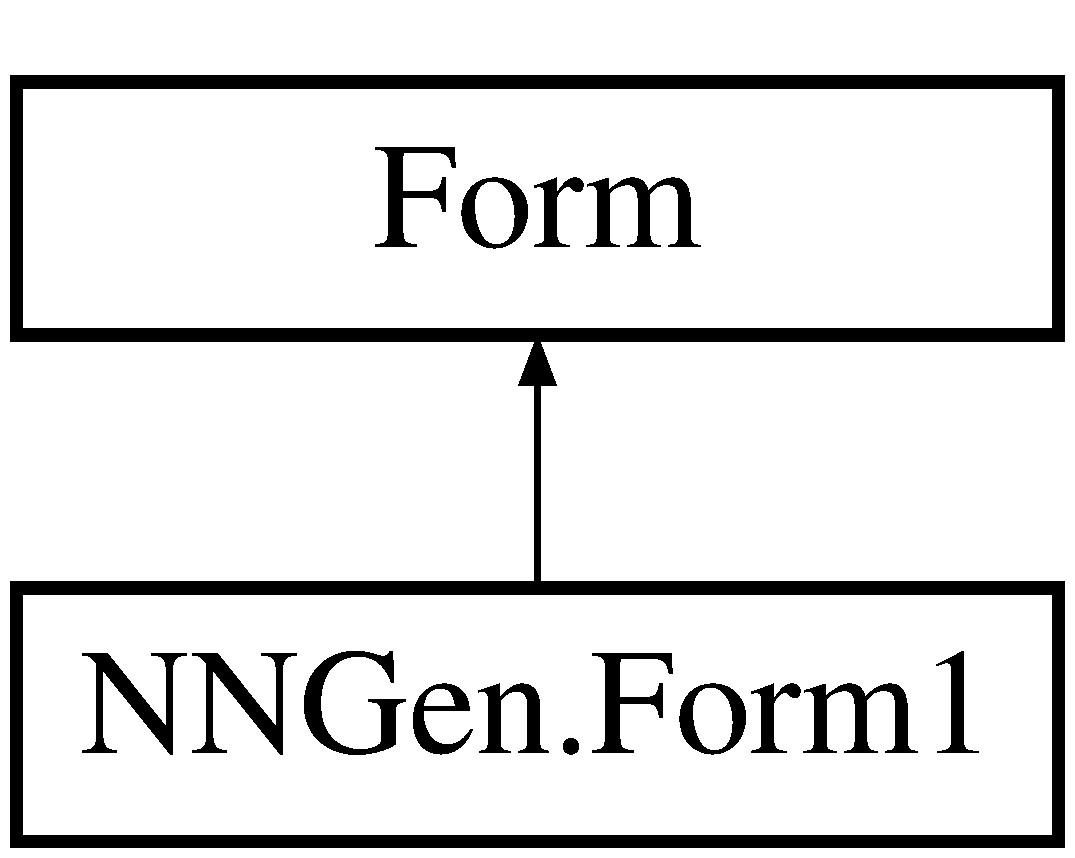
\includegraphics[height=2.000000cm]{class_n_n_gen_1_1_form1}
\end{center}
\end{figure}
\subsection*{Public Member Functions}
\begin{DoxyCompactItemize}
\item 
\hyperlink{class_n_n_gen_1_1_form1_ad7a3dddfefd46943cee8221a00e78a2d}{Form1} ()
\begin{DoxyCompactList}\small\item\em The constructor for the form \end{DoxyCompactList}\end{DoxyCompactItemize}
\subsection*{Protected Member Functions}
\begin{DoxyCompactItemize}
\item 
override void \hyperlink{class_n_n_gen_1_1_form1_a0c2f9c40cfcc62a50bfee5d9616845d4}{Dispose} (bool disposing)
\begin{DoxyCompactList}\small\item\em Clean up any resources being used. \end{DoxyCompactList}\end{DoxyCompactItemize}


\subsection{Detailed Description}
The main user interface form for testing the application Not much documentation is provided, as these aren\textquotesingle{}t meant to be public members. They are very straightforward, and can be used as example cod,e however. 



\subsection{Constructor \& Destructor Documentation}
\hypertarget{class_n_n_gen_1_1_form1_ad7a3dddfefd46943cee8221a00e78a2d}{}\index{N\+N\+Gen\+::\+Form1@{N\+N\+Gen\+::\+Form1}!Form1@{Form1}}
\index{Form1@{Form1}!N\+N\+Gen\+::\+Form1@{N\+N\+Gen\+::\+Form1}}
\subsubsection[{Form1()}]{\setlength{\rightskip}{0pt plus 5cm}N\+N\+Gen.\+Form1.\+Form1 (
\begin{DoxyParamCaption}
{}
\end{DoxyParamCaption}
)\hspace{0.3cm}{\ttfamily [inline]}}\label{class_n_n_gen_1_1_form1_ad7a3dddfefd46943cee8221a00e78a2d}


The constructor for the form 



\subsection{Member Function Documentation}
\hypertarget{class_n_n_gen_1_1_form1_a0c2f9c40cfcc62a50bfee5d9616845d4}{}\index{N\+N\+Gen\+::\+Form1@{N\+N\+Gen\+::\+Form1}!Dispose@{Dispose}}
\index{Dispose@{Dispose}!N\+N\+Gen\+::\+Form1@{N\+N\+Gen\+::\+Form1}}
\subsubsection[{Dispose(bool disposing)}]{\setlength{\rightskip}{0pt plus 5cm}override void N\+N\+Gen.\+Form1.\+Dispose (
\begin{DoxyParamCaption}
\item[{bool}]{disposing}
\end{DoxyParamCaption}
)\hspace{0.3cm}{\ttfamily [inline]}, {\ttfamily [protected]}}\label{class_n_n_gen_1_1_form1_a0c2f9c40cfcc62a50bfee5d9616845d4}


Clean up any resources being used. 


\begin{DoxyParams}{Parameters}
{\em disposing} & true if managed resources should be disposed; otherwise, false.\\
\hline
\end{DoxyParams}


The documentation for this class was generated from the following files\+:\begin{DoxyCompactItemize}
\item 
E\+:/\+Documents/\+Visual Studio 2013/\+Projects/\+Neural\+Network/\+N\+N\+Gen/\hyperlink{_form1_8cs}{Form1.\+cs}\item 
E\+:/\+Documents/\+Visual Studio 2013/\+Projects/\+Neural\+Network/\+N\+N\+Gen/\hyperlink{_form1_8_designer_8cs}{Form1.\+Designer.\+cs}\end{DoxyCompactItemize}

\hypertarget{class_n_n_gen_1_1_layer_setup}{}\section{N\+N\+Gen.\+Layer\+Setup Class Reference}
\label{class_n_n_gen_1_1_layer_setup}\index{N\+N\+Gen.\+Layer\+Setup@{N\+N\+Gen.\+Layer\+Setup}}


A pannel for setting up a single layer of the Neural Network  


Inheritance diagram for N\+N\+Gen.\+Layer\+Setup\+:\begin{figure}[H]
\begin{center}
\leavevmode
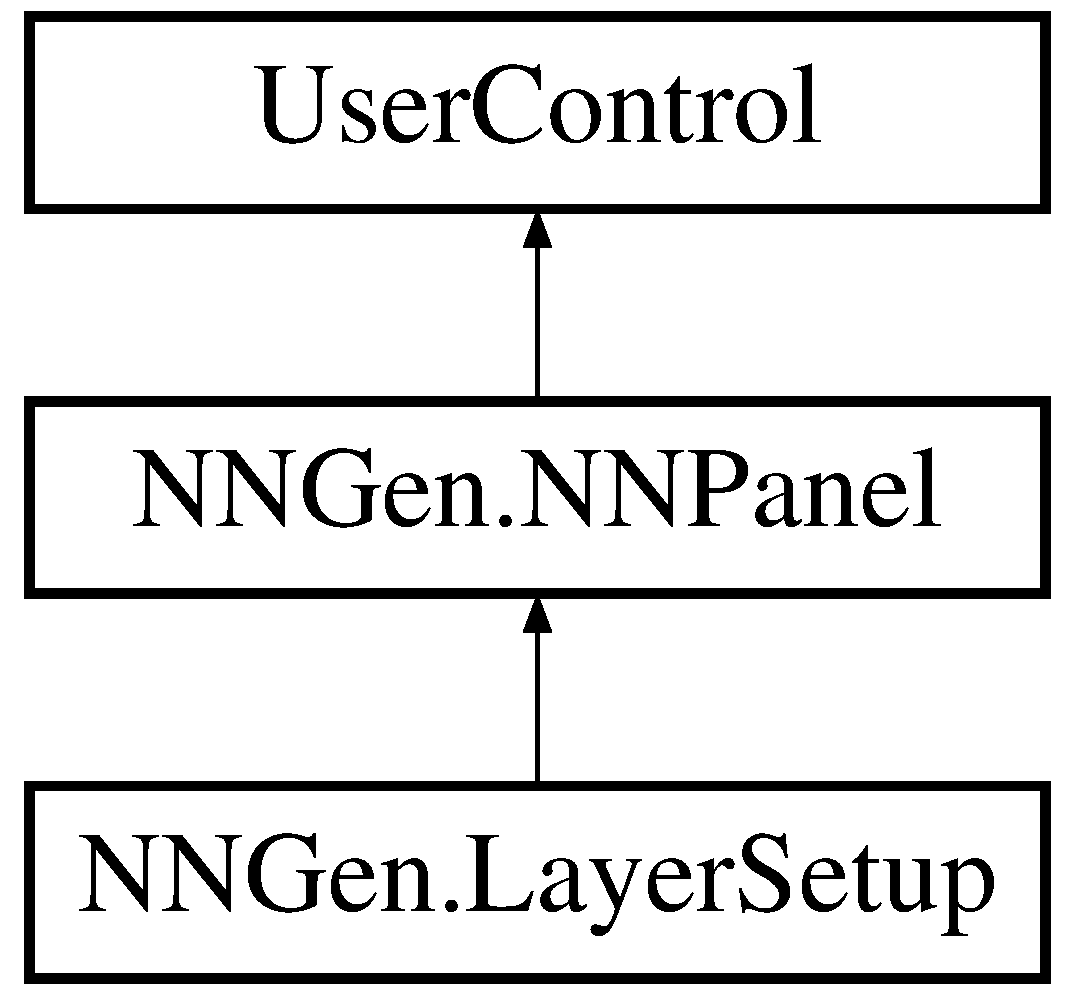
\includegraphics[height=3.000000cm]{class_n_n_gen_1_1_layer_setup}
\end{center}
\end{figure}
\subsection*{Public Member Functions}
\begin{DoxyCompactItemize}
\item 
\hyperlink{class_n_n_gen_1_1_layer_setup_a5daf76885695996275037fd51323d062}{Layer\+Setup} (string \+\_\+title\+String, bool \+\_\+bias\+Enabled, double \+\_\+bias\+Value, int \+\_\+num\+Neuron, bool \+\_\+thresholding\+Enabled, \hyperlink{class_n_n_gen_1_1_async_neuron_afe8460a52808d1587cbcc0a8e4e23b64}{Async\+Neuron.\+Neuron\+Activation\+Type} \+\_\+async\+Type, \hyperlink{class_n_n_gen_1_1_transfer_function_wrapper_aa338ffadb8fcdf76df75419374a51ff6}{Transfer\+Function\+Wrapper.\+Memory\+Activation\+Type} \+\_\+sync\+Type, bool \+\_\+is\+Sync\+Layer, bool \+\_\+is\+Last\+Layer)
\begin{DoxyCompactList}\small\item\em Construct the layer setup form \end{DoxyCompactList}\item 
override bool \hyperlink{class_n_n_gen_1_1_layer_setup_a0601d6640ad94c5e34316b60e70f8ede}{verify} ()
\begin{DoxyCompactList}\small\item\em The \hyperlink{class_n_n_gen_1_1_layer_setup_a0601d6640ad94c5e34316b60e70f8ede}{verify()} method implementation for this class. See N\+N\+Pannel.\+verify() for more documentation. \end{DoxyCompactList}\end{DoxyCompactItemize}
\subsection*{Protected Member Functions}
\begin{DoxyCompactItemize}
\item 
override void \hyperlink{class_n_n_gen_1_1_layer_setup_a3a9b3fe98e68a22d02ca7caf42800408}{Dispose} (bool disposing)
\begin{DoxyCompactList}\small\item\em Clean up any resources being used. \end{DoxyCompactList}\end{DoxyCompactItemize}
\subsection*{Properties}
\begin{DoxyCompactItemize}
\item 
int \hyperlink{class_n_n_gen_1_1_layer_setup_ad02db2fa93e561ffd181ad7824d6b296}{num\+Neurons}\hspace{0.3cm}{\ttfamily  \mbox{[}get\mbox{]}}
\begin{DoxyCompactList}\small\item\em The number of neurons in the layer \end{DoxyCompactList}\item 
double \hyperlink{class_n_n_gen_1_1_layer_setup_a44fec12782544a7b0ec9f9705251ebaf}{bias\+Value}\hspace{0.3cm}{\ttfamily  \mbox{[}get\mbox{]}}
\begin{DoxyCompactList}\small\item\em The bias value applied to the layer \end{DoxyCompactList}\item 
bool \hyperlink{class_n_n_gen_1_1_layer_setup_aba1fd67f0b1f840794b46dcd3626e05f}{bias\+Enabled}\hspace{0.3cm}{\ttfamily  \mbox{[}get\mbox{]}}
\begin{DoxyCompactList}\small\item\em A boolean representing whether the layer can have a bias node (disabled for the output layer) \end{DoxyCompactList}\item 
bool \hyperlink{class_n_n_gen_1_1_layer_setup_a8b5e8dd32a59d8ebb4956e3ddb6220b8}{thresholding\+Enabled}\hspace{0.3cm}{\ttfamily  \mbox{[}get\mbox{]}}
\begin{DoxyCompactList}\small\item\em A boolean representing whether thresholding is available for the layer (disabled for the input layer) \end{DoxyCompactList}\item 
bool \hyperlink{class_n_n_gen_1_1_layer_setup_a3c8d928b37fc46a8098bb9698dbd622c}{is\+Sync\+Layer}\hspace{0.3cm}{\ttfamily  \mbox{[}get\mbox{]}}
\begin{DoxyCompactList}\small\item\em A flag for whether this layer is synchronous \end{DoxyCompactList}\item 
bool \hyperlink{class_n_n_gen_1_1_layer_setup_a7c89db95e04b0f4b046786ba56b97b76}{is\+Last\+Layer}\hspace{0.3cm}{\ttfamily  \mbox{[}get\mbox{]}}
\begin{DoxyCompactList}\small\item\em A flag for whether this is the last layer in the network \end{DoxyCompactList}\item 
bool \hyperlink{class_n_n_gen_1_1_layer_setup_adbccceab05f4b3f3f7aba558408f4e94}{is\+Classifier}\hspace{0.3cm}{\ttfamily  \mbox{[}get\mbox{]}}
\begin{DoxyCompactList}\small\item\em A flag for whether this network should be a classification network as opposed to a regression network \end{DoxyCompactList}\item 
double\mbox{[}$\,$\mbox{]} \hyperlink{class_n_n_gen_1_1_layer_setup_afd7deda67d710ebec7628b2eec8f484b}{classifier\+Thresholds}\hspace{0.3cm}{\ttfamily  \mbox{[}get\mbox{]}}
\begin{DoxyCompactList}\small\item\em A structure for holding the thresholds for a classification network. If the network is a regression network, this item will be blank. \end{DoxyCompactList}\item 
\hyperlink{class_n_n_gen_1_1_async_neuron_afe8460a52808d1587cbcc0a8e4e23b64}{Async\+Neuron.\+Neuron\+Activation\+Type} \hyperlink{class_n_n_gen_1_1_layer_setup_a7b3a1f35136f4ba1abc63ef61d2733f3}{async\+Activation\+Type}\hspace{0.3cm}{\ttfamily  \mbox{[}get\mbox{]}}
\begin{DoxyCompactList}\small\item\em For an asynchronous network, the activation type for the layer \end{DoxyCompactList}\item 
\hyperlink{class_n_n_gen_1_1_transfer_function_wrapper_aa338ffadb8fcdf76df75419374a51ff6}{Transfer\+Function\+Wrapper.\+Memory\+Activation\+Type} \hyperlink{class_n_n_gen_1_1_layer_setup_a305c28b6f6a27e7f729362e63280e997}{sync\+Activation\+Type}\hspace{0.3cm}{\ttfamily  \mbox{[}get\mbox{]}}
\begin{DoxyCompactList}\small\item\em For a synchronous network, the activation type for the layer. \end{DoxyCompactList}\end{DoxyCompactItemize}


\subsection{Detailed Description}
A pannel for setting up a single layer of the Neural Network 



\subsection{Constructor \& Destructor Documentation}
\hypertarget{class_n_n_gen_1_1_layer_setup_a5daf76885695996275037fd51323d062}{}\index{N\+N\+Gen\+::\+Layer\+Setup@{N\+N\+Gen\+::\+Layer\+Setup}!Layer\+Setup@{Layer\+Setup}}
\index{Layer\+Setup@{Layer\+Setup}!N\+N\+Gen\+::\+Layer\+Setup@{N\+N\+Gen\+::\+Layer\+Setup}}
\subsubsection[{Layer\+Setup(string \+\_\+title\+String, bool \+\_\+bias\+Enabled, double \+\_\+bias\+Value, int \+\_\+num\+Neuron, bool \+\_\+thresholding\+Enabled, Async\+Neuron.\+Neuron\+Activation\+Type \+\_\+async\+Type, Transfer\+Function\+Wrapper.\+Memory\+Activation\+Type \+\_\+sync\+Type, bool \+\_\+is\+Sync\+Layer, bool \+\_\+is\+Last\+Layer)}]{\setlength{\rightskip}{0pt plus 5cm}N\+N\+Gen.\+Layer\+Setup.\+Layer\+Setup (
\begin{DoxyParamCaption}
\item[{string}]{\+\_\+title\+String, }
\item[{bool}]{\+\_\+bias\+Enabled, }
\item[{double}]{\+\_\+bias\+Value, }
\item[{int}]{\+\_\+num\+Neuron, }
\item[{bool}]{\+\_\+thresholding\+Enabled, }
\item[{{\bf Async\+Neuron.\+Neuron\+Activation\+Type}}]{\+\_\+async\+Type, }
\item[{{\bf Transfer\+Function\+Wrapper.\+Memory\+Activation\+Type}}]{\+\_\+sync\+Type, }
\item[{bool}]{\+\_\+is\+Sync\+Layer, }
\item[{bool}]{\+\_\+is\+Last\+Layer}
\end{DoxyParamCaption}
)\hspace{0.3cm}{\ttfamily [inline]}}\label{class_n_n_gen_1_1_layer_setup_a5daf76885695996275037fd51323d062}


Construct the layer setup form 


\begin{DoxyParams}{Parameters}
{\em \+\_\+title\+String} & The string to display in the title\\
\hline
{\em \+\_\+bias\+Enabled} & The seed value for whether the bias node is enabled for this layer or not\\
\hline
{\em \+\_\+bias\+Value} & The seed value for the bias value for this layer\\
\hline
{\em \+\_\+num\+Neuron} & The seed value for the number of neurons in the layer\\
\hline
{\em \+\_\+thresholding\+Enabled} & A flag for determing whether thresholding is enabled in this layer\\
\hline
{\em \+\_\+async\+Type} & For asynchronous networks, the seed value for the activation type. This parameter is ingored for synchronous networks\\
\hline
{\em \+\_\+sync\+Type} & For synchronous networks, the seed value for the activation type. This parameter is ignored for the asynchronous networks\\
\hline
{\em \+\_\+is\+Sync\+Layer} & A flag for setting whether this layer is synchronous or asynchronous\\
\hline
{\em \+\_\+is\+Last\+Layer} & A flag for setting whether this is the last layer in the network or not\\
\hline
\end{DoxyParams}


\subsection{Member Function Documentation}
\hypertarget{class_n_n_gen_1_1_layer_setup_a3a9b3fe98e68a22d02ca7caf42800408}{}\index{N\+N\+Gen\+::\+Layer\+Setup@{N\+N\+Gen\+::\+Layer\+Setup}!Dispose@{Dispose}}
\index{Dispose@{Dispose}!N\+N\+Gen\+::\+Layer\+Setup@{N\+N\+Gen\+::\+Layer\+Setup}}
\subsubsection[{Dispose(bool disposing)}]{\setlength{\rightskip}{0pt plus 5cm}override void N\+N\+Gen.\+Layer\+Setup.\+Dispose (
\begin{DoxyParamCaption}
\item[{bool}]{disposing}
\end{DoxyParamCaption}
)\hspace{0.3cm}{\ttfamily [inline]}, {\ttfamily [protected]}}\label{class_n_n_gen_1_1_layer_setup_a3a9b3fe98e68a22d02ca7caf42800408}


Clean up any resources being used. 


\begin{DoxyParams}{Parameters}
{\em disposing} & true if managed resources should be disposed; otherwise, false.\\
\hline
\end{DoxyParams}
\hypertarget{class_n_n_gen_1_1_layer_setup_a0601d6640ad94c5e34316b60e70f8ede}{}\index{N\+N\+Gen\+::\+Layer\+Setup@{N\+N\+Gen\+::\+Layer\+Setup}!verify@{verify}}
\index{verify@{verify}!N\+N\+Gen\+::\+Layer\+Setup@{N\+N\+Gen\+::\+Layer\+Setup}}
\subsubsection[{verify()}]{\setlength{\rightskip}{0pt plus 5cm}override bool N\+N\+Gen.\+Layer\+Setup.\+verify (
\begin{DoxyParamCaption}
{}
\end{DoxyParamCaption}
)\hspace{0.3cm}{\ttfamily [inline]}, {\ttfamily [virtual]}}\label{class_n_n_gen_1_1_layer_setup_a0601d6640ad94c5e34316b60e70f8ede}


The \hyperlink{class_n_n_gen_1_1_layer_setup_a0601d6640ad94c5e34316b60e70f8ede}{verify()} method implementation for this class. See N\+N\+Pannel.\+verify() for more documentation. 

\begin{DoxyReturn}{Returns}

\end{DoxyReturn}


Reimplemented from \hyperlink{class_n_n_gen_1_1_n_n_panel_a36e3bcf90c9e561e8502eac6f884582a}{N\+N\+Gen.\+N\+N\+Panel}.



\subsection{Property Documentation}
\hypertarget{class_n_n_gen_1_1_layer_setup_a7b3a1f35136f4ba1abc63ef61d2733f3}{}\index{N\+N\+Gen\+::\+Layer\+Setup@{N\+N\+Gen\+::\+Layer\+Setup}!async\+Activation\+Type@{async\+Activation\+Type}}
\index{async\+Activation\+Type@{async\+Activation\+Type}!N\+N\+Gen\+::\+Layer\+Setup@{N\+N\+Gen\+::\+Layer\+Setup}}
\subsubsection[{async\+Activation\+Type}]{\setlength{\rightskip}{0pt plus 5cm}{\bf Async\+Neuron.\+Neuron\+Activation\+Type} N\+N\+Gen.\+Layer\+Setup.\+async\+Activation\+Type\hspace{0.3cm}{\ttfamily [get]}}\label{class_n_n_gen_1_1_layer_setup_a7b3a1f35136f4ba1abc63ef61d2733f3}


For an asynchronous network, the activation type for the layer 

\hypertarget{class_n_n_gen_1_1_layer_setup_aba1fd67f0b1f840794b46dcd3626e05f}{}\index{N\+N\+Gen\+::\+Layer\+Setup@{N\+N\+Gen\+::\+Layer\+Setup}!bias\+Enabled@{bias\+Enabled}}
\index{bias\+Enabled@{bias\+Enabled}!N\+N\+Gen\+::\+Layer\+Setup@{N\+N\+Gen\+::\+Layer\+Setup}}
\subsubsection[{bias\+Enabled}]{\setlength{\rightskip}{0pt plus 5cm}bool N\+N\+Gen.\+Layer\+Setup.\+bias\+Enabled\hspace{0.3cm}{\ttfamily [get]}}\label{class_n_n_gen_1_1_layer_setup_aba1fd67f0b1f840794b46dcd3626e05f}


A boolean representing whether the layer can have a bias node (disabled for the output layer) 

\hypertarget{class_n_n_gen_1_1_layer_setup_a44fec12782544a7b0ec9f9705251ebaf}{}\index{N\+N\+Gen\+::\+Layer\+Setup@{N\+N\+Gen\+::\+Layer\+Setup}!bias\+Value@{bias\+Value}}
\index{bias\+Value@{bias\+Value}!N\+N\+Gen\+::\+Layer\+Setup@{N\+N\+Gen\+::\+Layer\+Setup}}
\subsubsection[{bias\+Value}]{\setlength{\rightskip}{0pt plus 5cm}double N\+N\+Gen.\+Layer\+Setup.\+bias\+Value\hspace{0.3cm}{\ttfamily [get]}}\label{class_n_n_gen_1_1_layer_setup_a44fec12782544a7b0ec9f9705251ebaf}


The bias value applied to the layer 

\hypertarget{class_n_n_gen_1_1_layer_setup_afd7deda67d710ebec7628b2eec8f484b}{}\index{N\+N\+Gen\+::\+Layer\+Setup@{N\+N\+Gen\+::\+Layer\+Setup}!classifier\+Thresholds@{classifier\+Thresholds}}
\index{classifier\+Thresholds@{classifier\+Thresholds}!N\+N\+Gen\+::\+Layer\+Setup@{N\+N\+Gen\+::\+Layer\+Setup}}
\subsubsection[{classifier\+Thresholds}]{\setlength{\rightskip}{0pt plus 5cm}double \mbox{[}$\,$\mbox{]} N\+N\+Gen.\+Layer\+Setup.\+classifier\+Thresholds\hspace{0.3cm}{\ttfamily [get]}}\label{class_n_n_gen_1_1_layer_setup_afd7deda67d710ebec7628b2eec8f484b}


A structure for holding the thresholds for a classification network. If the network is a regression network, this item will be blank. 

\hypertarget{class_n_n_gen_1_1_layer_setup_adbccceab05f4b3f3f7aba558408f4e94}{}\index{N\+N\+Gen\+::\+Layer\+Setup@{N\+N\+Gen\+::\+Layer\+Setup}!is\+Classifier@{is\+Classifier}}
\index{is\+Classifier@{is\+Classifier}!N\+N\+Gen\+::\+Layer\+Setup@{N\+N\+Gen\+::\+Layer\+Setup}}
\subsubsection[{is\+Classifier}]{\setlength{\rightskip}{0pt plus 5cm}bool N\+N\+Gen.\+Layer\+Setup.\+is\+Classifier\hspace{0.3cm}{\ttfamily [get]}}\label{class_n_n_gen_1_1_layer_setup_adbccceab05f4b3f3f7aba558408f4e94}


A flag for whether this network should be a classification network as opposed to a regression network 

\hypertarget{class_n_n_gen_1_1_layer_setup_a7c89db95e04b0f4b046786ba56b97b76}{}\index{N\+N\+Gen\+::\+Layer\+Setup@{N\+N\+Gen\+::\+Layer\+Setup}!is\+Last\+Layer@{is\+Last\+Layer}}
\index{is\+Last\+Layer@{is\+Last\+Layer}!N\+N\+Gen\+::\+Layer\+Setup@{N\+N\+Gen\+::\+Layer\+Setup}}
\subsubsection[{is\+Last\+Layer}]{\setlength{\rightskip}{0pt plus 5cm}bool N\+N\+Gen.\+Layer\+Setup.\+is\+Last\+Layer\hspace{0.3cm}{\ttfamily [get]}}\label{class_n_n_gen_1_1_layer_setup_a7c89db95e04b0f4b046786ba56b97b76}


A flag for whether this is the last layer in the network 

\hypertarget{class_n_n_gen_1_1_layer_setup_a3c8d928b37fc46a8098bb9698dbd622c}{}\index{N\+N\+Gen\+::\+Layer\+Setup@{N\+N\+Gen\+::\+Layer\+Setup}!is\+Sync\+Layer@{is\+Sync\+Layer}}
\index{is\+Sync\+Layer@{is\+Sync\+Layer}!N\+N\+Gen\+::\+Layer\+Setup@{N\+N\+Gen\+::\+Layer\+Setup}}
\subsubsection[{is\+Sync\+Layer}]{\setlength{\rightskip}{0pt plus 5cm}bool N\+N\+Gen.\+Layer\+Setup.\+is\+Sync\+Layer\hspace{0.3cm}{\ttfamily [get]}}\label{class_n_n_gen_1_1_layer_setup_a3c8d928b37fc46a8098bb9698dbd622c}


A flag for whether this layer is synchronous 

\hypertarget{class_n_n_gen_1_1_layer_setup_ad02db2fa93e561ffd181ad7824d6b296}{}\index{N\+N\+Gen\+::\+Layer\+Setup@{N\+N\+Gen\+::\+Layer\+Setup}!num\+Neurons@{num\+Neurons}}
\index{num\+Neurons@{num\+Neurons}!N\+N\+Gen\+::\+Layer\+Setup@{N\+N\+Gen\+::\+Layer\+Setup}}
\subsubsection[{num\+Neurons}]{\setlength{\rightskip}{0pt plus 5cm}int N\+N\+Gen.\+Layer\+Setup.\+num\+Neurons\hspace{0.3cm}{\ttfamily [get]}}\label{class_n_n_gen_1_1_layer_setup_ad02db2fa93e561ffd181ad7824d6b296}


The number of neurons in the layer 

\hypertarget{class_n_n_gen_1_1_layer_setup_a305c28b6f6a27e7f729362e63280e997}{}\index{N\+N\+Gen\+::\+Layer\+Setup@{N\+N\+Gen\+::\+Layer\+Setup}!sync\+Activation\+Type@{sync\+Activation\+Type}}
\index{sync\+Activation\+Type@{sync\+Activation\+Type}!N\+N\+Gen\+::\+Layer\+Setup@{N\+N\+Gen\+::\+Layer\+Setup}}
\subsubsection[{sync\+Activation\+Type}]{\setlength{\rightskip}{0pt plus 5cm}{\bf Transfer\+Function\+Wrapper.\+Memory\+Activation\+Type} N\+N\+Gen.\+Layer\+Setup.\+sync\+Activation\+Type\hspace{0.3cm}{\ttfamily [get]}}\label{class_n_n_gen_1_1_layer_setup_a305c28b6f6a27e7f729362e63280e997}


For a synchronous network, the activation type for the layer. 

\hypertarget{class_n_n_gen_1_1_layer_setup_a8b5e8dd32a59d8ebb4956e3ddb6220b8}{}\index{N\+N\+Gen\+::\+Layer\+Setup@{N\+N\+Gen\+::\+Layer\+Setup}!thresholding\+Enabled@{thresholding\+Enabled}}
\index{thresholding\+Enabled@{thresholding\+Enabled}!N\+N\+Gen\+::\+Layer\+Setup@{N\+N\+Gen\+::\+Layer\+Setup}}
\subsubsection[{thresholding\+Enabled}]{\setlength{\rightskip}{0pt plus 5cm}bool N\+N\+Gen.\+Layer\+Setup.\+thresholding\+Enabled\hspace{0.3cm}{\ttfamily [get]}}\label{class_n_n_gen_1_1_layer_setup_a8b5e8dd32a59d8ebb4956e3ddb6220b8}


A boolean representing whether thresholding is available for the layer (disabled for the input layer) 



The documentation for this class was generated from the following files\+:\begin{DoxyCompactItemize}
\item 
E\+:/\+Documents/\+Visual Studio 2013/\+Projects/\+Neural\+Network/\+N\+N\+Gen/\hyperlink{_layer_setup_8cs}{Layer\+Setup.\+cs}\item 
E\+:/\+Documents/\+Visual Studio 2013/\+Projects/\+Neural\+Network/\+N\+N\+Gen/\hyperlink{_layer_setup_8_designer_8cs}{Layer\+Setup.\+Designer.\+cs}\end{DoxyCompactItemize}

\hypertarget{class_n_n_gen_1_1_main_form}{}\section{N\+N\+Gen.\+Main\+Form Class Reference}
\label{class_n_n_gen_1_1_main_form}\index{N\+N\+Gen.\+Main\+Form@{N\+N\+Gen.\+Main\+Form}}


The main window for the application  


Inheritance diagram for N\+N\+Gen.\+Main\+Form\+:\begin{figure}[H]
\begin{center}
\leavevmode
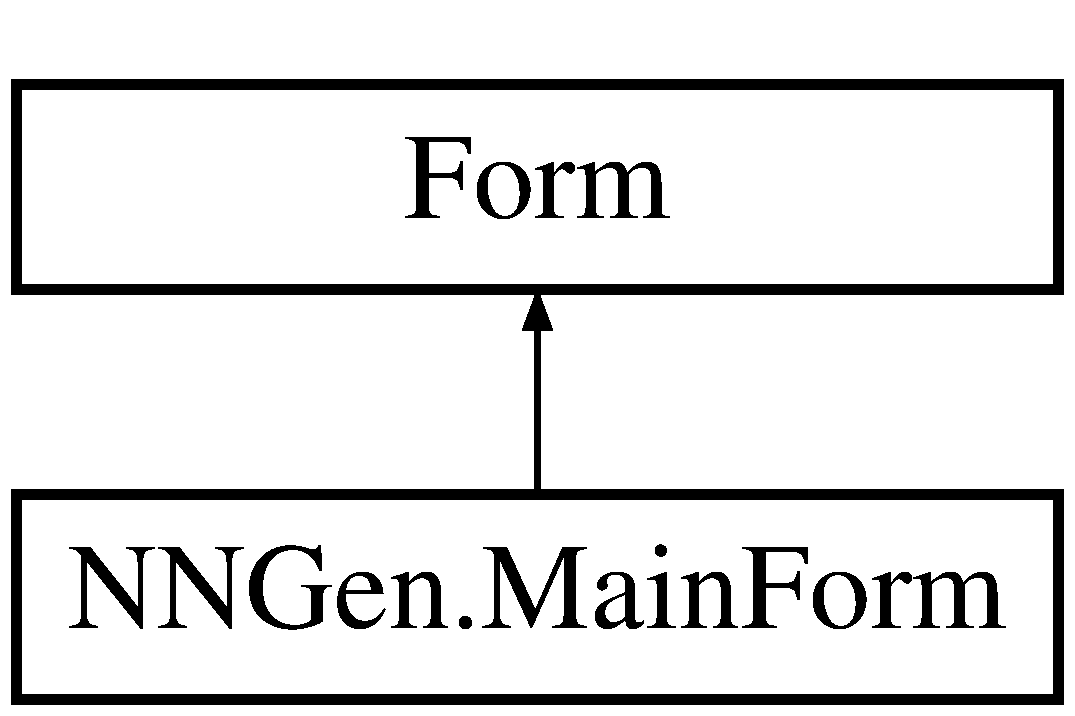
\includegraphics[height=2.000000cm]{class_n_n_gen_1_1_main_form}
\end{center}
\end{figure}
\subsection*{Public Member Functions}
\begin{DoxyCompactItemize}
\item 
\hyperlink{class_n_n_gen_1_1_main_form_a369d3b409380f302157457e6621badc9}{Main\+Form} ()
\begin{DoxyCompactList}\small\item\em Creates a \hyperlink{class_n_n_gen_1_1_main_form}{Main\+Form} \end{DoxyCompactList}\end{DoxyCompactItemize}
\subsection*{Protected Member Functions}
\begin{DoxyCompactItemize}
\item 
override void \hyperlink{class_n_n_gen_1_1_main_form_a9d1a2820f8c6e68cfe9a09d6fd4ca30f}{Dispose} (bool disposing)
\begin{DoxyCompactList}\small\item\em Clean up any resources being used. \end{DoxyCompactList}\end{DoxyCompactItemize}


\subsection{Detailed Description}
The main window for the application 



\subsection{Constructor \& Destructor Documentation}
\hypertarget{class_n_n_gen_1_1_main_form_a369d3b409380f302157457e6621badc9}{}\index{N\+N\+Gen\+::\+Main\+Form@{N\+N\+Gen\+::\+Main\+Form}!Main\+Form@{Main\+Form}}
\index{Main\+Form@{Main\+Form}!N\+N\+Gen\+::\+Main\+Form@{N\+N\+Gen\+::\+Main\+Form}}
\subsubsection[{Main\+Form()}]{\setlength{\rightskip}{0pt plus 5cm}N\+N\+Gen.\+Main\+Form.\+Main\+Form (
\begin{DoxyParamCaption}
{}
\end{DoxyParamCaption}
)\hspace{0.3cm}{\ttfamily [inline]}}\label{class_n_n_gen_1_1_main_form_a369d3b409380f302157457e6621badc9}


Creates a \hyperlink{class_n_n_gen_1_1_main_form}{Main\+Form} 



\subsection{Member Function Documentation}
\hypertarget{class_n_n_gen_1_1_main_form_a9d1a2820f8c6e68cfe9a09d6fd4ca30f}{}\index{N\+N\+Gen\+::\+Main\+Form@{N\+N\+Gen\+::\+Main\+Form}!Dispose@{Dispose}}
\index{Dispose@{Dispose}!N\+N\+Gen\+::\+Main\+Form@{N\+N\+Gen\+::\+Main\+Form}}
\subsubsection[{Dispose(bool disposing)}]{\setlength{\rightskip}{0pt plus 5cm}override void N\+N\+Gen.\+Main\+Form.\+Dispose (
\begin{DoxyParamCaption}
\item[{bool}]{disposing}
\end{DoxyParamCaption}
)\hspace{0.3cm}{\ttfamily [inline]}, {\ttfamily [protected]}}\label{class_n_n_gen_1_1_main_form_a9d1a2820f8c6e68cfe9a09d6fd4ca30f}


Clean up any resources being used. 


\begin{DoxyParams}{Parameters}
{\em disposing} & true if managed resources should be disposed; otherwise, false.\\
\hline
\end{DoxyParams}


The documentation for this class was generated from the following files\+:\begin{DoxyCompactItemize}
\item 
E\+:/\+Documents/\+Visual Studio 2013/\+Projects/\+Neural\+Network/\+N\+N\+Gen/\hyperlink{_main_form_8cs}{Main\+Form.\+cs}\item 
E\+:/\+Documents/\+Visual Studio 2013/\+Projects/\+Neural\+Network/\+N\+N\+Gen/\hyperlink{_main_form_8_designer_8cs}{Main\+Form.\+Designer.\+cs}\end{DoxyCompactItemize}

\hypertarget{class_n_n_gen_1_1_network_setup}{}\section{N\+N\+Gen.\+Network\+Setup Class Reference}
\label{class_n_n_gen_1_1_network_setup}\index{N\+N\+Gen.\+Network\+Setup@{N\+N\+Gen.\+Network\+Setup}}


A screen for setting up the number of layers in the network  


Inheritance diagram for N\+N\+Gen.\+Network\+Setup\+:\begin{figure}[H]
\begin{center}
\leavevmode
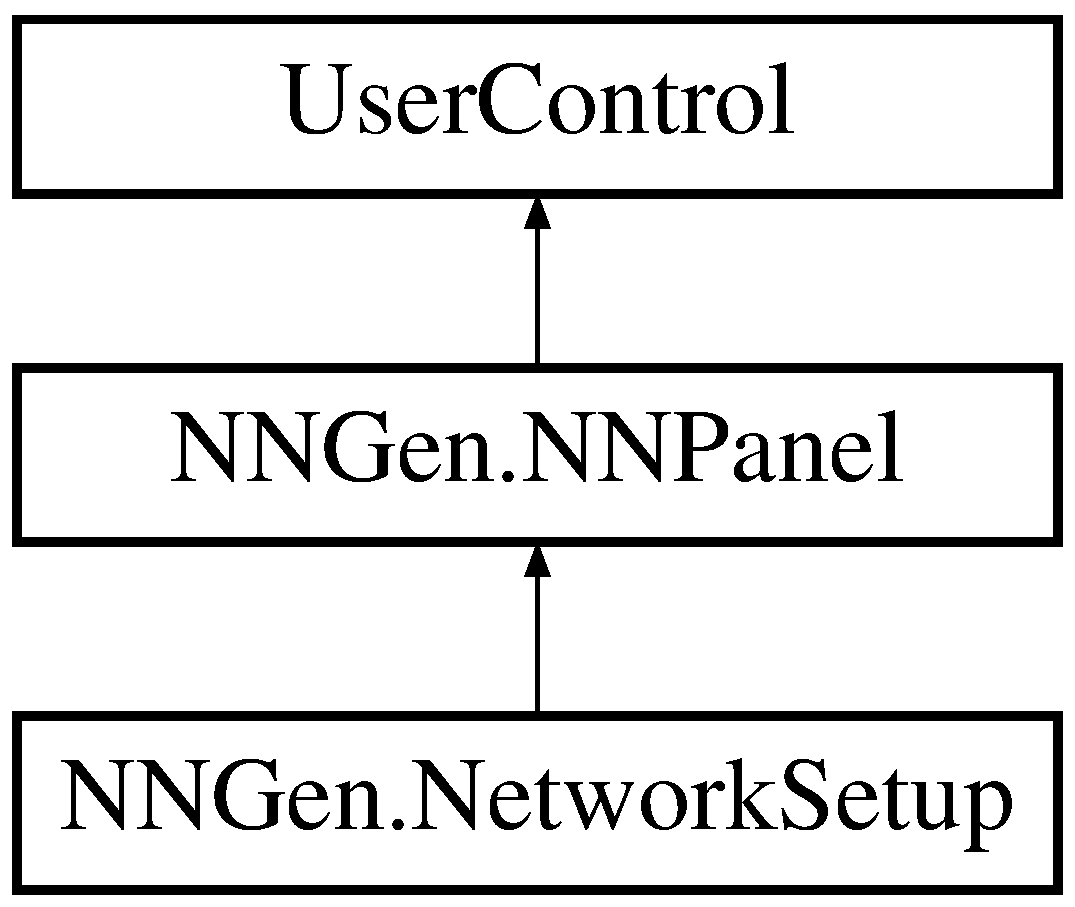
\includegraphics[height=3.000000cm]{class_n_n_gen_1_1_network_setup}
\end{center}
\end{figure}
\subsection*{Public Member Functions}
\begin{DoxyCompactItemize}
\item 
\hyperlink{class_n_n_gen_1_1_network_setup_ae51ae2c3bb47dab47afd6d022e07a230}{Network\+Setup} (int \+\_\+num\+Hidden\+Layers)
\begin{DoxyCompactList}\small\item\em Initialize a \hyperlink{class_n_n_gen_1_1_network_setup}{Network\+Setup} pannel \end{DoxyCompactList}\item 
override bool \hyperlink{class_n_n_gen_1_1_network_setup_a0fadf5361f2bea6d04cbfe70012c3365}{verify} ()
\begin{DoxyCompactList}\small\item\em The \hyperlink{class_n_n_gen_1_1_network_setup_a0fadf5361f2bea6d04cbfe70012c3365}{verify()} method implementation for this class. See N\+N\+Pannel.\+verify() for more documentation. \end{DoxyCompactList}\end{DoxyCompactItemize}
\subsection*{Protected Member Functions}
\begin{DoxyCompactItemize}
\item 
override void \hyperlink{class_n_n_gen_1_1_network_setup_a53c3ce61507af95b37e90045529eb086}{Dispose} (bool disposing)
\begin{DoxyCompactList}\small\item\em Clean up any resources being used. \end{DoxyCompactList}\end{DoxyCompactItemize}
\subsection*{Properties}
\begin{DoxyCompactItemize}
\item 
int \hyperlink{class_n_n_gen_1_1_network_setup_a1a90afb18c0fbb167d46337505d8e63e}{num\+Hidden\+Layers}\hspace{0.3cm}{\ttfamily  \mbox{[}get\mbox{]}}
\begin{DoxyCompactList}\small\item\em The number of hidden layers in the network \end{DoxyCompactList}\end{DoxyCompactItemize}


\subsection{Detailed Description}
A screen for setting up the number of layers in the network 



\subsection{Constructor \& Destructor Documentation}
\hypertarget{class_n_n_gen_1_1_network_setup_ae51ae2c3bb47dab47afd6d022e07a230}{}\index{N\+N\+Gen\+::\+Network\+Setup@{N\+N\+Gen\+::\+Network\+Setup}!Network\+Setup@{Network\+Setup}}
\index{Network\+Setup@{Network\+Setup}!N\+N\+Gen\+::\+Network\+Setup@{N\+N\+Gen\+::\+Network\+Setup}}
\subsubsection[{Network\+Setup(int \+\_\+num\+Hidden\+Layers)}]{\setlength{\rightskip}{0pt plus 5cm}N\+N\+Gen.\+Network\+Setup.\+Network\+Setup (
\begin{DoxyParamCaption}
\item[{int}]{\+\_\+num\+Hidden\+Layers}
\end{DoxyParamCaption}
)\hspace{0.3cm}{\ttfamily [inline]}}\label{class_n_n_gen_1_1_network_setup_ae51ae2c3bb47dab47afd6d022e07a230}


Initialize a \hyperlink{class_n_n_gen_1_1_network_setup}{Network\+Setup} pannel 


\begin{DoxyParams}{Parameters}
{\em \+\_\+num\+Hidden\+Layers} & The seed value for the number of hidden layers in the network\\
\hline
\end{DoxyParams}


\subsection{Member Function Documentation}
\hypertarget{class_n_n_gen_1_1_network_setup_a53c3ce61507af95b37e90045529eb086}{}\index{N\+N\+Gen\+::\+Network\+Setup@{N\+N\+Gen\+::\+Network\+Setup}!Dispose@{Dispose}}
\index{Dispose@{Dispose}!N\+N\+Gen\+::\+Network\+Setup@{N\+N\+Gen\+::\+Network\+Setup}}
\subsubsection[{Dispose(bool disposing)}]{\setlength{\rightskip}{0pt plus 5cm}override void N\+N\+Gen.\+Network\+Setup.\+Dispose (
\begin{DoxyParamCaption}
\item[{bool}]{disposing}
\end{DoxyParamCaption}
)\hspace{0.3cm}{\ttfamily [inline]}, {\ttfamily [protected]}}\label{class_n_n_gen_1_1_network_setup_a53c3ce61507af95b37e90045529eb086}


Clean up any resources being used. 


\begin{DoxyParams}{Parameters}
{\em disposing} & true if managed resources should be disposed; otherwise, false.\\
\hline
\end{DoxyParams}
\hypertarget{class_n_n_gen_1_1_network_setup_a0fadf5361f2bea6d04cbfe70012c3365}{}\index{N\+N\+Gen\+::\+Network\+Setup@{N\+N\+Gen\+::\+Network\+Setup}!verify@{verify}}
\index{verify@{verify}!N\+N\+Gen\+::\+Network\+Setup@{N\+N\+Gen\+::\+Network\+Setup}}
\subsubsection[{verify()}]{\setlength{\rightskip}{0pt plus 5cm}override bool N\+N\+Gen.\+Network\+Setup.\+verify (
\begin{DoxyParamCaption}
{}
\end{DoxyParamCaption}
)\hspace{0.3cm}{\ttfamily [inline]}, {\ttfamily [virtual]}}\label{class_n_n_gen_1_1_network_setup_a0fadf5361f2bea6d04cbfe70012c3365}


The \hyperlink{class_n_n_gen_1_1_network_setup_a0fadf5361f2bea6d04cbfe70012c3365}{verify()} method implementation for this class. See N\+N\+Pannel.\+verify() for more documentation. 

\begin{DoxyReturn}{Returns}

\end{DoxyReturn}


Reimplemented from \hyperlink{class_n_n_gen_1_1_n_n_panel_a36e3bcf90c9e561e8502eac6f884582a}{N\+N\+Gen.\+N\+N\+Panel}.



\subsection{Property Documentation}
\hypertarget{class_n_n_gen_1_1_network_setup_a1a90afb18c0fbb167d46337505d8e63e}{}\index{N\+N\+Gen\+::\+Network\+Setup@{N\+N\+Gen\+::\+Network\+Setup}!num\+Hidden\+Layers@{num\+Hidden\+Layers}}
\index{num\+Hidden\+Layers@{num\+Hidden\+Layers}!N\+N\+Gen\+::\+Network\+Setup@{N\+N\+Gen\+::\+Network\+Setup}}
\subsubsection[{num\+Hidden\+Layers}]{\setlength{\rightskip}{0pt plus 5cm}int N\+N\+Gen.\+Network\+Setup.\+num\+Hidden\+Layers\hspace{0.3cm}{\ttfamily [get]}}\label{class_n_n_gen_1_1_network_setup_a1a90afb18c0fbb167d46337505d8e63e}


The number of hidden layers in the network 



The documentation for this class was generated from the following files\+:\begin{DoxyCompactItemize}
\item 
E\+:/\+Documents/\+Visual Studio 2013/\+Projects/\+Neural\+Network/\+N\+N\+Gen/\hyperlink{_network_setup_8cs}{Network\+Setup.\+cs}\item 
E\+:/\+Documents/\+Visual Studio 2013/\+Projects/\+Neural\+Network/\+N\+N\+Gen/\hyperlink{_network_setup_8_designer_8cs}{Network\+Setup.\+Designer.\+cs}\end{DoxyCompactItemize}

\hypertarget{class_n_n_gen_1_1_n_n_panel}{}\section{N\+N\+Gen.\+N\+N\+Panel Class Reference}
\label{class_n_n_gen_1_1_n_n_panel}\index{N\+N\+Gen.\+N\+N\+Panel@{N\+N\+Gen.\+N\+N\+Panel}}


An abstraction of a single screen (pannel) in the U\+I  


Inheritance diagram for N\+N\+Gen.\+N\+N\+Panel\+:\begin{figure}[H]
\begin{center}
\leavevmode
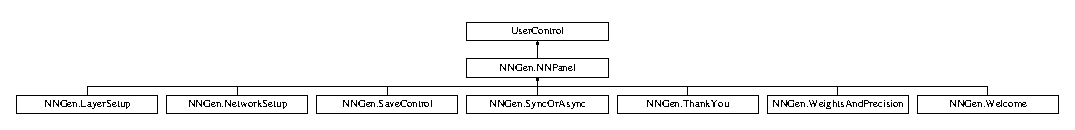
\includegraphics[height=1.297297cm]{class_n_n_gen_1_1_n_n_panel}
\end{center}
\end{figure}
\subsection*{Public Member Functions}
\begin{DoxyCompactItemize}
\item 
\hyperlink{class_n_n_gen_1_1_n_n_panel_abc0696f7f309efb402b07085676ca562}{N\+N\+Panel} ()
\begin{DoxyCompactList}\small\item\em A blank constructor for the pannel \end{DoxyCompactList}\item 
void \hyperlink{class_n_n_gen_1_1_n_n_panel_a593ac509de9ee22792c68900e8cf8843}{resize} (int width, int height)
\begin{DoxyCompactList}\small\item\em Resizes the pannel \end{DoxyCompactList}\item 
virtual bool \hyperlink{class_n_n_gen_1_1_n_n_panel_a36e3bcf90c9e561e8502eac6f884582a}{verify} ()
\begin{DoxyCompactList}\small\item\em A method used to determine whether the form has had all of its data successfully entered. This method should be overridden in child classes to return true if all data has been successfully entered, and false otherwise. \end{DoxyCompactList}\end{DoxyCompactItemize}
\subsection*{Protected Member Functions}
\begin{DoxyCompactItemize}
\item 
override void \hyperlink{class_n_n_gen_1_1_n_n_panel_ad0b5586daded54ef00a8afb8e6f3b4d9}{Dispose} (bool disposing)
\begin{DoxyCompactList}\small\item\em Clean up any resources being used. \end{DoxyCompactList}\end{DoxyCompactItemize}


\subsection{Detailed Description}
An abstraction of a single screen (pannel) in the U\+I 



\subsection{Constructor \& Destructor Documentation}
\hypertarget{class_n_n_gen_1_1_n_n_panel_abc0696f7f309efb402b07085676ca562}{}\index{N\+N\+Gen\+::\+N\+N\+Panel@{N\+N\+Gen\+::\+N\+N\+Panel}!N\+N\+Panel@{N\+N\+Panel}}
\index{N\+N\+Panel@{N\+N\+Panel}!N\+N\+Gen\+::\+N\+N\+Panel@{N\+N\+Gen\+::\+N\+N\+Panel}}
\subsubsection[{N\+N\+Panel()}]{\setlength{\rightskip}{0pt plus 5cm}N\+N\+Gen.\+N\+N\+Panel.\+N\+N\+Panel (
\begin{DoxyParamCaption}
{}
\end{DoxyParamCaption}
)\hspace{0.3cm}{\ttfamily [inline]}}\label{class_n_n_gen_1_1_n_n_panel_abc0696f7f309efb402b07085676ca562}


A blank constructor for the pannel 



\subsection{Member Function Documentation}
\hypertarget{class_n_n_gen_1_1_n_n_panel_ad0b5586daded54ef00a8afb8e6f3b4d9}{}\index{N\+N\+Gen\+::\+N\+N\+Panel@{N\+N\+Gen\+::\+N\+N\+Panel}!Dispose@{Dispose}}
\index{Dispose@{Dispose}!N\+N\+Gen\+::\+N\+N\+Panel@{N\+N\+Gen\+::\+N\+N\+Panel}}
\subsubsection[{Dispose(bool disposing)}]{\setlength{\rightskip}{0pt plus 5cm}override void N\+N\+Gen.\+N\+N\+Panel.\+Dispose (
\begin{DoxyParamCaption}
\item[{bool}]{disposing}
\end{DoxyParamCaption}
)\hspace{0.3cm}{\ttfamily [inline]}, {\ttfamily [protected]}}\label{class_n_n_gen_1_1_n_n_panel_ad0b5586daded54ef00a8afb8e6f3b4d9}


Clean up any resources being used. 


\begin{DoxyParams}{Parameters}
{\em disposing} & true if managed resources should be disposed; otherwise, false.\\
\hline
\end{DoxyParams}
\hypertarget{class_n_n_gen_1_1_n_n_panel_a593ac509de9ee22792c68900e8cf8843}{}\index{N\+N\+Gen\+::\+N\+N\+Panel@{N\+N\+Gen\+::\+N\+N\+Panel}!resize@{resize}}
\index{resize@{resize}!N\+N\+Gen\+::\+N\+N\+Panel@{N\+N\+Gen\+::\+N\+N\+Panel}}
\subsubsection[{resize(int width, int height)}]{\setlength{\rightskip}{0pt plus 5cm}void N\+N\+Gen.\+N\+N\+Panel.\+resize (
\begin{DoxyParamCaption}
\item[{int}]{width, }
\item[{int}]{height}
\end{DoxyParamCaption}
)\hspace{0.3cm}{\ttfamily [inline]}}\label{class_n_n_gen_1_1_n_n_panel_a593ac509de9ee22792c68900e8cf8843}


Resizes the pannel 


\begin{DoxyParams}{Parameters}
{\em width} & The new width of the pannel\\
\hline
{\em height} & \\
\hline
\end{DoxyParams}
\hypertarget{class_n_n_gen_1_1_n_n_panel_a36e3bcf90c9e561e8502eac6f884582a}{}\index{N\+N\+Gen\+::\+N\+N\+Panel@{N\+N\+Gen\+::\+N\+N\+Panel}!verify@{verify}}
\index{verify@{verify}!N\+N\+Gen\+::\+N\+N\+Panel@{N\+N\+Gen\+::\+N\+N\+Panel}}
\subsubsection[{verify()}]{\setlength{\rightskip}{0pt plus 5cm}virtual bool N\+N\+Gen.\+N\+N\+Panel.\+verify (
\begin{DoxyParamCaption}
{}
\end{DoxyParamCaption}
)\hspace{0.3cm}{\ttfamily [inline]}, {\ttfamily [virtual]}}\label{class_n_n_gen_1_1_n_n_panel_a36e3bcf90c9e561e8502eac6f884582a}


A method used to determine whether the form has had all of its data successfully entered. This method should be overridden in child classes to return true if all data has been successfully entered, and false otherwise. 

\begin{DoxyReturn}{Returns}

\end{DoxyReturn}


Reimplemented in \hyperlink{class_n_n_gen_1_1_layer_setup_a0601d6640ad94c5e34316b60e70f8ede}{N\+N\+Gen.\+Layer\+Setup}, \hyperlink{class_n_n_gen_1_1_weights_and_precision_a55e25affc261256144c0cd9866a63b7a}{N\+N\+Gen.\+Weights\+And\+Precision}, \hyperlink{class_n_n_gen_1_1_save_control_a9802bdb470edb0fbc0fe3d7b04863f6c}{N\+N\+Gen.\+Save\+Control}, \hyperlink{class_n_n_gen_1_1_network_setup_a0fadf5361f2bea6d04cbfe70012c3365}{N\+N\+Gen.\+Network\+Setup}, and \hyperlink{class_n_n_gen_1_1_sync_or_async_a43e1723039a0485fe09f6f374eb48620}{N\+N\+Gen.\+Sync\+Or\+Async}.



The documentation for this class was generated from the following files\+:\begin{DoxyCompactItemize}
\item 
E\+:/\+Documents/\+Visual Studio 2013/\+Projects/\+Neural\+Network/\+N\+N\+Gen/\hyperlink{_n_n_panel_8cs}{N\+N\+Panel.\+cs}\item 
E\+:/\+Documents/\+Visual Studio 2013/\+Projects/\+Neural\+Network/\+N\+N\+Gen/\hyperlink{_n_n_panel_8_designer_8cs}{N\+N\+Panel.\+Designer.\+cs}\end{DoxyCompactItemize}

\hypertarget{class_n_n_gen_1_1_panel_container}{}\section{N\+N\+Gen.\+Panel\+Container Class Reference}
\label{class_n_n_gen_1_1_panel_container}\index{N\+N\+Gen.\+Panel\+Container@{N\+N\+Gen.\+Panel\+Container}}


A container for holding the list of panels to show the user  


\subsection*{Public Member Functions}
\begin{DoxyCompactItemize}
\item 
\hyperlink{class_n_n_gen_1_1_panel_container_aff90f9069cacfacb87c98c4683c00a08}{Panel\+Container} (List$<$ \hyperlink{class_n_n_gen_1_1_n_n_panel}{N\+N\+Panel} $>$ \+\_\+panels)
\begin{DoxyCompactList}\small\item\em Create a \hyperlink{class_n_n_gen_1_1_panel_container}{Panel\+Container} \end{DoxyCompactList}\item 
\hyperlink{class_n_n_gen_1_1_n_n_panel}{N\+N\+Panel} \hyperlink{class_n_n_gen_1_1_panel_container_abcf640c5145757f67e0e39529e62d9a3}{advance} (int width, int height)
\begin{DoxyCompactList}\small\item\em Attempt to advance to the next panel. If the current panel has had all of its data entered correctly, then this method returns the next form resized to (width, height) If there is an error, the current panel will be returned \end{DoxyCompactList}\item 
\hyperlink{class_n_n_gen_1_1_n_n_panel}{N\+N\+Panel} \hyperlink{class_n_n_gen_1_1_panel_container_aa1082f9ed06b22a03b46c0228d814f05}{previous} (int width, int height)
\begin{DoxyCompactList}\small\item\em Safely returns the previous panel in the list resized to (Width, Height) If this method is called on the first panel in the list, then the first panel is returned. \end{DoxyCompactList}\item 
\hyperlink{class_n_n_gen_1_1_n_n_panel}{N\+N\+Panel} \hyperlink{class_n_n_gen_1_1_panel_container_ad9762df6a510b1b7af423720da0f6130}{current} (int width, int height)
\begin{DoxyCompactList}\small\item\em Return the current panel, resized to (Width, Height) \end{DoxyCompactList}\item 
\hyperlink{class_n_n_gen_1_1_n_n_panel}{N\+N\+Panel} \hyperlink{class_n_n_gen_1_1_panel_container_abb4eb5b543b584a98049316c23f20c8e}{current} ()
\begin{DoxyCompactList}\small\item\em Return the current panel without resizing \end{DoxyCompactList}\item 
void \hyperlink{class_n_n_gen_1_1_panel_container_a38332e7d9ea9d92eff375cf40a6458a4}{clear\+To\+End} (int index)
\begin{DoxyCompactList}\small\item\em Removes all panels from the list with an index greater than or equal to (index) \end{DoxyCompactList}\item 
bool \hyperlink{class_n_n_gen_1_1_panel_container_a181928c6c73958241a1db08f21cd1257}{is\+End} ()
\begin{DoxyCompactList}\small\item\em Returns whether the cursor index is at the end of the list \end{DoxyCompactList}\end{DoxyCompactItemize}
\subsection*{Properties}
\begin{DoxyCompactItemize}
\item 
List$<$ \hyperlink{class_n_n_gen_1_1_n_n_panel}{N\+N\+Panel} $>$ \hyperlink{class_n_n_gen_1_1_panel_container_a31f3e003f5a5fa87884d717e2c01f310}{panels}\hspace{0.3cm}{\ttfamily  \mbox{[}get, set\mbox{]}}
\begin{DoxyCompactList}\small\item\em The list of panels to be shown to the user \end{DoxyCompactList}\item 
int \hyperlink{class_n_n_gen_1_1_panel_container_a2134090074da8e94c15b7ed69fe75d06}{current\+Panel\+Index}\hspace{0.3cm}{\ttfamily  \mbox{[}get, set\mbox{]}}
\begin{DoxyCompactList}\small\item\em The index of the current panel being shown \end{DoxyCompactList}\end{DoxyCompactItemize}


\subsection{Detailed Description}
A container for holding the list of panels to show the user 



\subsection{Constructor \& Destructor Documentation}
\hypertarget{class_n_n_gen_1_1_panel_container_aff90f9069cacfacb87c98c4683c00a08}{}\index{N\+N\+Gen\+::\+Panel\+Container@{N\+N\+Gen\+::\+Panel\+Container}!Panel\+Container@{Panel\+Container}}
\index{Panel\+Container@{Panel\+Container}!N\+N\+Gen\+::\+Panel\+Container@{N\+N\+Gen\+::\+Panel\+Container}}
\subsubsection[{Panel\+Container(\+List$<$ N\+N\+Panel $>$ \+\_\+panels)}]{\setlength{\rightskip}{0pt plus 5cm}N\+N\+Gen.\+Panel\+Container.\+Panel\+Container (
\begin{DoxyParamCaption}
\item[{List$<$ {\bf N\+N\+Panel} $>$}]{\+\_\+panels}
\end{DoxyParamCaption}
)\hspace{0.3cm}{\ttfamily [inline]}}\label{class_n_n_gen_1_1_panel_container_aff90f9069cacfacb87c98c4683c00a08}


Create a \hyperlink{class_n_n_gen_1_1_panel_container}{Panel\+Container} 


\begin{DoxyParams}{Parameters}
{\em \+\_\+panels} & The list of panels to be shown to the user\\
\hline
\end{DoxyParams}


\subsection{Member Function Documentation}
\hypertarget{class_n_n_gen_1_1_panel_container_abcf640c5145757f67e0e39529e62d9a3}{}\index{N\+N\+Gen\+::\+Panel\+Container@{N\+N\+Gen\+::\+Panel\+Container}!advance@{advance}}
\index{advance@{advance}!N\+N\+Gen\+::\+Panel\+Container@{N\+N\+Gen\+::\+Panel\+Container}}
\subsubsection[{advance(int width, int height)}]{\setlength{\rightskip}{0pt plus 5cm}{\bf N\+N\+Panel} N\+N\+Gen.\+Panel\+Container.\+advance (
\begin{DoxyParamCaption}
\item[{int}]{width, }
\item[{int}]{height}
\end{DoxyParamCaption}
)\hspace{0.3cm}{\ttfamily [inline]}}\label{class_n_n_gen_1_1_panel_container_abcf640c5145757f67e0e39529e62d9a3}


Attempt to advance to the next panel. If the current panel has had all of its data entered correctly, then this method returns the next form resized to (width, height) If there is an error, the current panel will be returned 


\begin{DoxyParams}{Parameters}
{\em width} & The width of the panel to return\\
\hline
{\em height} & The height of the panel to return\\
\hline
\end{DoxyParams}
\begin{DoxyReturn}{Returns}
The next panel in the list, or the current panel
\end{DoxyReturn}
\hypertarget{class_n_n_gen_1_1_panel_container_a38332e7d9ea9d92eff375cf40a6458a4}{}\index{N\+N\+Gen\+::\+Panel\+Container@{N\+N\+Gen\+::\+Panel\+Container}!clear\+To\+End@{clear\+To\+End}}
\index{clear\+To\+End@{clear\+To\+End}!N\+N\+Gen\+::\+Panel\+Container@{N\+N\+Gen\+::\+Panel\+Container}}
\subsubsection[{clear\+To\+End(int index)}]{\setlength{\rightskip}{0pt plus 5cm}void N\+N\+Gen.\+Panel\+Container.\+clear\+To\+End (
\begin{DoxyParamCaption}
\item[{int}]{index}
\end{DoxyParamCaption}
)\hspace{0.3cm}{\ttfamily [inline]}}\label{class_n_n_gen_1_1_panel_container_a38332e7d9ea9d92eff375cf40a6458a4}


Removes all panels from the list with an index greater than or equal to (index) 


\begin{DoxyParams}{Parameters}
{\em index} & The starting index to remove\\
\hline
\end{DoxyParams}
\hypertarget{class_n_n_gen_1_1_panel_container_ad9762df6a510b1b7af423720da0f6130}{}\index{N\+N\+Gen\+::\+Panel\+Container@{N\+N\+Gen\+::\+Panel\+Container}!current@{current}}
\index{current@{current}!N\+N\+Gen\+::\+Panel\+Container@{N\+N\+Gen\+::\+Panel\+Container}}
\subsubsection[{current(int width, int height)}]{\setlength{\rightskip}{0pt plus 5cm}{\bf N\+N\+Panel} N\+N\+Gen.\+Panel\+Container.\+current (
\begin{DoxyParamCaption}
\item[{int}]{width, }
\item[{int}]{height}
\end{DoxyParamCaption}
)\hspace{0.3cm}{\ttfamily [inline]}}\label{class_n_n_gen_1_1_panel_container_ad9762df6a510b1b7af423720da0f6130}


Return the current panel, resized to (Width, Height) 


\begin{DoxyParams}{Parameters}
{\em width} & The width of the panel to return\\
\hline
{\em height} & The height of the panel to return\\
\hline
\end{DoxyParams}
\begin{DoxyReturn}{Returns}
The current panel
\end{DoxyReturn}
\hypertarget{class_n_n_gen_1_1_panel_container_abb4eb5b543b584a98049316c23f20c8e}{}\index{N\+N\+Gen\+::\+Panel\+Container@{N\+N\+Gen\+::\+Panel\+Container}!current@{current}}
\index{current@{current}!N\+N\+Gen\+::\+Panel\+Container@{N\+N\+Gen\+::\+Panel\+Container}}
\subsubsection[{current()}]{\setlength{\rightskip}{0pt plus 5cm}{\bf N\+N\+Panel} N\+N\+Gen.\+Panel\+Container.\+current (
\begin{DoxyParamCaption}
{}
\end{DoxyParamCaption}
)\hspace{0.3cm}{\ttfamily [inline]}}\label{class_n_n_gen_1_1_panel_container_abb4eb5b543b584a98049316c23f20c8e}


Return the current panel without resizing 

\begin{DoxyReturn}{Returns}
The current panel
\end{DoxyReturn}
\hypertarget{class_n_n_gen_1_1_panel_container_a181928c6c73958241a1db08f21cd1257}{}\index{N\+N\+Gen\+::\+Panel\+Container@{N\+N\+Gen\+::\+Panel\+Container}!is\+End@{is\+End}}
\index{is\+End@{is\+End}!N\+N\+Gen\+::\+Panel\+Container@{N\+N\+Gen\+::\+Panel\+Container}}
\subsubsection[{is\+End()}]{\setlength{\rightskip}{0pt plus 5cm}bool N\+N\+Gen.\+Panel\+Container.\+is\+End (
\begin{DoxyParamCaption}
{}
\end{DoxyParamCaption}
)\hspace{0.3cm}{\ttfamily [inline]}}\label{class_n_n_gen_1_1_panel_container_a181928c6c73958241a1db08f21cd1257}


Returns whether the cursor index is at the end of the list 

\begin{DoxyReturn}{Returns}
True if the cursor is at the end of the list
\end{DoxyReturn}
\hypertarget{class_n_n_gen_1_1_panel_container_aa1082f9ed06b22a03b46c0228d814f05}{}\index{N\+N\+Gen\+::\+Panel\+Container@{N\+N\+Gen\+::\+Panel\+Container}!previous@{previous}}
\index{previous@{previous}!N\+N\+Gen\+::\+Panel\+Container@{N\+N\+Gen\+::\+Panel\+Container}}
\subsubsection[{previous(int width, int height)}]{\setlength{\rightskip}{0pt plus 5cm}{\bf N\+N\+Panel} N\+N\+Gen.\+Panel\+Container.\+previous (
\begin{DoxyParamCaption}
\item[{int}]{width, }
\item[{int}]{height}
\end{DoxyParamCaption}
)\hspace{0.3cm}{\ttfamily [inline]}}\label{class_n_n_gen_1_1_panel_container_aa1082f9ed06b22a03b46c0228d814f05}


Safely returns the previous panel in the list resized to (Width, Height) If this method is called on the first panel in the list, then the first panel is returned. 


\begin{DoxyParams}{Parameters}
{\em width} & The width of the panel to return\\
\hline
{\em height} & The height of the panel to return\\
\hline
\end{DoxyParams}
\begin{DoxyReturn}{Returns}
The previous panel in the list, or the first panel
\end{DoxyReturn}


\subsection{Property Documentation}
\hypertarget{class_n_n_gen_1_1_panel_container_a2134090074da8e94c15b7ed69fe75d06}{}\index{N\+N\+Gen\+::\+Panel\+Container@{N\+N\+Gen\+::\+Panel\+Container}!current\+Panel\+Index@{current\+Panel\+Index}}
\index{current\+Panel\+Index@{current\+Panel\+Index}!N\+N\+Gen\+::\+Panel\+Container@{N\+N\+Gen\+::\+Panel\+Container}}
\subsubsection[{current\+Panel\+Index}]{\setlength{\rightskip}{0pt plus 5cm}int N\+N\+Gen.\+Panel\+Container.\+current\+Panel\+Index\hspace{0.3cm}{\ttfamily [get]}, {\ttfamily [set]}}\label{class_n_n_gen_1_1_panel_container_a2134090074da8e94c15b7ed69fe75d06}


The index of the current panel being shown 

\hypertarget{class_n_n_gen_1_1_panel_container_a31f3e003f5a5fa87884d717e2c01f310}{}\index{N\+N\+Gen\+::\+Panel\+Container@{N\+N\+Gen\+::\+Panel\+Container}!panels@{panels}}
\index{panels@{panels}!N\+N\+Gen\+::\+Panel\+Container@{N\+N\+Gen\+::\+Panel\+Container}}
\subsubsection[{panels}]{\setlength{\rightskip}{0pt plus 5cm}List$<${\bf N\+N\+Panel}$>$ N\+N\+Gen.\+Panel\+Container.\+panels\hspace{0.3cm}{\ttfamily [get]}, {\ttfamily [set]}}\label{class_n_n_gen_1_1_panel_container_a31f3e003f5a5fa87884d717e2c01f310}


The list of panels to be shown to the user 



The documentation for this class was generated from the following file\+:\begin{DoxyCompactItemize}
\item 
E\+:/\+Documents/\+Visual Studio 2013/\+Projects/\+Neural\+Network/\+N\+N\+Gen/\hyperlink{_panel_container_8cs}{Panel\+Container.\+cs}\end{DoxyCompactItemize}

\hypertarget{class_n_n_gen_1_1_port}{}\section{N\+N\+Gen.\+Port Class Reference}
\label{class_n_n_gen_1_1_port}\index{N\+N\+Gen.\+Port@{N\+N\+Gen.\+Port}}


A datatype representing a port in an entity  


\subsection*{Public Types}
\begin{DoxyCompactItemize}
\item 
enum \hyperlink{class_n_n_gen_1_1_port_ac3b8f11a7a6bd6872e6954b64721d90c}{port\+Direction} \{ \hyperlink{class_n_n_gen_1_1_port_ac3b8f11a7a6bd6872e6954b64721d90cac86ee0d9d7ed3e7b4fdbf486fa6c0ebb}{port\+Direction.\+I\+N}, 
\hyperlink{class_n_n_gen_1_1_port_ac3b8f11a7a6bd6872e6954b64721d90caef373774188a51f80463f37b6bd9e83a}{port\+Direction.\+O\+U\+T}, 
\hyperlink{class_n_n_gen_1_1_port_ac3b8f11a7a6bd6872e6954b64721d90ca0c93f5d83bbb636236e9610d01e4f3cd}{port\+Direction.\+I\+N\+O\+U\+T}, 
\hyperlink{class_n_n_gen_1_1_port_ac3b8f11a7a6bd6872e6954b64721d90ca17de626bcae5109bb2f7a66dfc4a8a1d}{port\+Direction.\+B\+U\+F\+F\+E\+R}
 \}\begin{DoxyCompactList}\small\item\em An enumeration representing the directions for the port \end{DoxyCompactList}
\end{DoxyCompactItemize}
\subsection*{Public Member Functions}
\begin{DoxyCompactItemize}
\item 
\hyperlink{class_n_n_gen_1_1_port_a2b360d742ee9a3b11e4c9f95b8a7a956}{Port} (\hyperlink{class_n_n_gen_1_1_port_ac3b8f11a7a6bd6872e6954b64721d90c}{port\+Direction} \+\_\+dir, string \+\_\+name, Utilities.\+V\+H\+D\+L\+Data\+Type \+\_\+type, int \+\_\+top, int \+\_\+bottom)
\begin{DoxyCompactList}\small\item\em The constructor for a port. \end{DoxyCompactList}\item 
string \hyperlink{class_n_n_gen_1_1_port_adc50095d3117b0a845e223c5d4502bf1}{V\+H\+D\+L\+String} (bool is\+Last)
\begin{DoxyCompactList}\small\item\em Returns a string used to declare the port Example\+: C\+L\+K\+: I\+N S\+T\+D\+\_\+\+L\+O\+G\+I\+C; \end{DoxyCompactList}\item 
\hyperlink{class_n_n_gen_1_1_signal}{Signal} \hyperlink{class_n_n_gen_1_1_port_ab58db29cb073ac7297104720f1580214}{to\+Signal} (string new\+Name)
\begin{DoxyCompactList}\small\item\em Returns a signal with the same properties of this port, except for the new name \end{DoxyCompactList}\item 
void \hyperlink{class_n_n_gen_1_1_port_a7bbd5a0006e1004d9cdaaf82be58fe85}{rename} (string new\+Name)
\begin{DoxyCompactList}\small\item\em Changes the name of the signal \end{DoxyCompactList}\item 
void \hyperlink{class_n_n_gen_1_1_port_ad830585db8a043e70c9210797dc80500}{set\+Direction} (\hyperlink{class_n_n_gen_1_1_port_ac3b8f11a7a6bd6872e6954b64721d90c}{Port.\+port\+Direction} dir)
\begin{DoxyCompactList}\small\item\em Change the direction of the port \end{DoxyCompactList}\item 
\hyperlink{class_n_n_gen_1_1_port}{Port} \hyperlink{class_n_n_gen_1_1_port_a0dbe21338296f8a5e624b9fe4bbb001f}{copy} ()
\begin{DoxyCompactList}\small\item\em Copy the definition of the port to another port struct \end{DoxyCompactList}\end{DoxyCompactItemize}
\subsection*{Properties}
\begin{DoxyCompactItemize}
\item 
\hyperlink{class_n_n_gen_1_1_port_ac3b8f11a7a6bd6872e6954b64721d90c}{port\+Direction} \hyperlink{class_n_n_gen_1_1_port_a68b34b101d99494b7fa7bcb78608a6bf}{direction}\hspace{0.3cm}{\ttfamily  \mbox{[}get\mbox{]}}
\begin{DoxyCompactList}\small\item\em The direction of this particular port \end{DoxyCompactList}\item 
string \hyperlink{class_n_n_gen_1_1_port_a0fc8ebe56a544edec825980f9961ed6d}{port\+Name}\hspace{0.3cm}{\ttfamily  \mbox{[}get\mbox{]}}
\begin{DoxyCompactList}\small\item\em The V\+H\+D\+L name of the particular port \end{DoxyCompactList}\item 
Utilities.\+V\+H\+D\+L\+Data\+Type \hyperlink{class_n_n_gen_1_1_port_a2b45b890a0e945e39d37a1cc596d1d20}{type}\hspace{0.3cm}{\ttfamily  \mbox{[}get\mbox{]}}
\begin{DoxyCompactList}\small\item\em The datatype of the particular port (see Utilities.\+V\+H\+D\+L\+Data\+Type) \end{DoxyCompactList}\item 
int \hyperlink{class_n_n_gen_1_1_port_ad68cf9376f181c135381671f67f03149}{top}\hspace{0.3cm}{\ttfamily  \mbox{[}get\mbox{]}}
\begin{DoxyCompactList}\small\item\em The top number in the (X D\+O\+W\+N\+T\+O Y) statement signifying the width of the signal \end{DoxyCompactList}\item 
int \hyperlink{class_n_n_gen_1_1_port_a7bf74261a0fc7d2574c45332a301dcb3}{bottom}\hspace{0.3cm}{\ttfamily  \mbox{[}get\mbox{]}}
\begin{DoxyCompactList}\small\item\em The bottom number in the (X D\+O\+W\+N\+T\+O Y) statement signifying the width of the signal \end{DoxyCompactList}\end{DoxyCompactItemize}


\subsection{Detailed Description}
A datatype representing a port in an entity 



\subsection{Member Enumeration Documentation}
\hypertarget{class_n_n_gen_1_1_port_ac3b8f11a7a6bd6872e6954b64721d90c}{}\index{N\+N\+Gen\+::\+Port@{N\+N\+Gen\+::\+Port}!port\+Direction@{port\+Direction}}
\index{port\+Direction@{port\+Direction}!N\+N\+Gen\+::\+Port@{N\+N\+Gen\+::\+Port}}
\subsubsection[{port\+Direction}]{\setlength{\rightskip}{0pt plus 5cm}enum {\bf N\+N\+Gen.\+Port.\+port\+Direction}\hspace{0.3cm}{\ttfamily [strong]}}\label{class_n_n_gen_1_1_port_ac3b8f11a7a6bd6872e6954b64721d90c}


An enumeration representing the directions for the port 

\begin{Desc}
\item[Enumerator]\par
\begin{description}
\index{I\+N@{I\+N}!N\+N\+Gen\+::\+Port@{N\+N\+Gen\+::\+Port}}\index{N\+N\+Gen\+::\+Port@{N\+N\+Gen\+::\+Port}!I\+N@{I\+N}}\item[{\em 
\hypertarget{class_n_n_gen_1_1_port_ac3b8f11a7a6bd6872e6954b64721d90cac86ee0d9d7ed3e7b4fdbf486fa6c0ebb}{}I\+N\label{class_n_n_gen_1_1_port_ac3b8f11a7a6bd6872e6954b64721d90cac86ee0d9d7ed3e7b4fdbf486fa6c0ebb}
}]Input port \index{O\+U\+T@{O\+U\+T}!N\+N\+Gen\+::\+Port@{N\+N\+Gen\+::\+Port}}\index{N\+N\+Gen\+::\+Port@{N\+N\+Gen\+::\+Port}!O\+U\+T@{O\+U\+T}}\item[{\em 
\hypertarget{class_n_n_gen_1_1_port_ac3b8f11a7a6bd6872e6954b64721d90caef373774188a51f80463f37b6bd9e83a}{}O\+U\+T\label{class_n_n_gen_1_1_port_ac3b8f11a7a6bd6872e6954b64721d90caef373774188a51f80463f37b6bd9e83a}
}]Output port \index{I\+N\+O\+U\+T@{I\+N\+O\+U\+T}!N\+N\+Gen\+::\+Port@{N\+N\+Gen\+::\+Port}}\index{N\+N\+Gen\+::\+Port@{N\+N\+Gen\+::\+Port}!I\+N\+O\+U\+T@{I\+N\+O\+U\+T}}\item[{\em 
\hypertarget{class_n_n_gen_1_1_port_ac3b8f11a7a6bd6872e6954b64721d90ca0c93f5d83bbb636236e9610d01e4f3cd}{}I\+N\+O\+U\+T\label{class_n_n_gen_1_1_port_ac3b8f11a7a6bd6872e6954b64721d90ca0c93f5d83bbb636236e9610d01e4f3cd}
}]In\+Out port \index{B\+U\+F\+F\+E\+R@{B\+U\+F\+F\+E\+R}!N\+N\+Gen\+::\+Port@{N\+N\+Gen\+::\+Port}}\index{N\+N\+Gen\+::\+Port@{N\+N\+Gen\+::\+Port}!B\+U\+F\+F\+E\+R@{B\+U\+F\+F\+E\+R}}\item[{\em 
\hypertarget{class_n_n_gen_1_1_port_ac3b8f11a7a6bd6872e6954b64721d90ca17de626bcae5109bb2f7a66dfc4a8a1d}{}B\+U\+F\+F\+E\+R\label{class_n_n_gen_1_1_port_ac3b8f11a7a6bd6872e6954b64721d90ca17de626bcae5109bb2f7a66dfc4a8a1d}
}]Buffer port \end{description}
\end{Desc}


\subsection{Constructor \& Destructor Documentation}
\hypertarget{class_n_n_gen_1_1_port_a2b360d742ee9a3b11e4c9f95b8a7a956}{}\index{N\+N\+Gen\+::\+Port@{N\+N\+Gen\+::\+Port}!Port@{Port}}
\index{Port@{Port}!N\+N\+Gen\+::\+Port@{N\+N\+Gen\+::\+Port}}
\subsubsection[{Port(port\+Direction \+\_\+dir, string \+\_\+name, Utilities.\+V\+H\+D\+L\+Data\+Type \+\_\+type, int \+\_\+top, int \+\_\+bottom)}]{\setlength{\rightskip}{0pt plus 5cm}N\+N\+Gen.\+Port.\+Port (
\begin{DoxyParamCaption}
\item[{{\bf port\+Direction}}]{\+\_\+dir, }
\item[{string}]{\+\_\+name, }
\item[{Utilities.\+V\+H\+D\+L\+Data\+Type}]{\+\_\+type, }
\item[{int}]{\+\_\+top, }
\item[{int}]{\+\_\+bottom}
\end{DoxyParamCaption}
)\hspace{0.3cm}{\ttfamily [inline]}}\label{class_n_n_gen_1_1_port_a2b360d742ee9a3b11e4c9f95b8a7a956}


The constructor for a port. 


\begin{DoxyParams}{Parameters}
{\em \+\_\+dir} & the direction of the port (See port\+Direction)\\
\hline
{\em \+\_\+name} & the V\+H\+D\+L name of the port\\
\hline
{\em \+\_\+type} & the V\+H\+D\+L datatype of the port\\
\hline
{\em \+\_\+top} & The upper limit for the port (X in X D\+O\+W\+N\+T\+O Y)\\
\hline
{\em \+\_\+bottom} & The lower limit for the port (Y in X D\+O\+W\+N\+T\+O Y)\\
\hline
\end{DoxyParams}


\subsection{Member Function Documentation}
\hypertarget{class_n_n_gen_1_1_port_a0dbe21338296f8a5e624b9fe4bbb001f}{}\index{N\+N\+Gen\+::\+Port@{N\+N\+Gen\+::\+Port}!copy@{copy}}
\index{copy@{copy}!N\+N\+Gen\+::\+Port@{N\+N\+Gen\+::\+Port}}
\subsubsection[{copy()}]{\setlength{\rightskip}{0pt plus 5cm}{\bf Port} N\+N\+Gen.\+Port.\+copy (
\begin{DoxyParamCaption}
{}
\end{DoxyParamCaption}
)\hspace{0.3cm}{\ttfamily [inline]}}\label{class_n_n_gen_1_1_port_a0dbe21338296f8a5e624b9fe4bbb001f}


Copy the definition of the port to another port struct 

\begin{DoxyReturn}{Returns}
A copy of the current port
\end{DoxyReturn}
\hypertarget{class_n_n_gen_1_1_port_a7bbd5a0006e1004d9cdaaf82be58fe85}{}\index{N\+N\+Gen\+::\+Port@{N\+N\+Gen\+::\+Port}!rename@{rename}}
\index{rename@{rename}!N\+N\+Gen\+::\+Port@{N\+N\+Gen\+::\+Port}}
\subsubsection[{rename(string new\+Name)}]{\setlength{\rightskip}{0pt plus 5cm}void N\+N\+Gen.\+Port.\+rename (
\begin{DoxyParamCaption}
\item[{string}]{new\+Name}
\end{DoxyParamCaption}
)\hspace{0.3cm}{\ttfamily [inline]}}\label{class_n_n_gen_1_1_port_a7bbd5a0006e1004d9cdaaf82be58fe85}


Changes the name of the signal 


\begin{DoxyParams}{Parameters}
{\em new\+Name} & \\
\hline
\end{DoxyParams}
\hypertarget{class_n_n_gen_1_1_port_ad830585db8a043e70c9210797dc80500}{}\index{N\+N\+Gen\+::\+Port@{N\+N\+Gen\+::\+Port}!set\+Direction@{set\+Direction}}
\index{set\+Direction@{set\+Direction}!N\+N\+Gen\+::\+Port@{N\+N\+Gen\+::\+Port}}
\subsubsection[{set\+Direction(\+Port.\+port\+Direction dir)}]{\setlength{\rightskip}{0pt plus 5cm}void N\+N\+Gen.\+Port.\+set\+Direction (
\begin{DoxyParamCaption}
\item[{{\bf Port.\+port\+Direction}}]{dir}
\end{DoxyParamCaption}
)\hspace{0.3cm}{\ttfamily [inline]}}\label{class_n_n_gen_1_1_port_ad830585db8a043e70c9210797dc80500}


Change the direction of the port 


\begin{DoxyParams}{Parameters}
{\em dir} & The new direction of the port\\
\hline
\end{DoxyParams}
\hypertarget{class_n_n_gen_1_1_port_ab58db29cb073ac7297104720f1580214}{}\index{N\+N\+Gen\+::\+Port@{N\+N\+Gen\+::\+Port}!to\+Signal@{to\+Signal}}
\index{to\+Signal@{to\+Signal}!N\+N\+Gen\+::\+Port@{N\+N\+Gen\+::\+Port}}
\subsubsection[{to\+Signal(string new\+Name)}]{\setlength{\rightskip}{0pt plus 5cm}{\bf Signal} N\+N\+Gen.\+Port.\+to\+Signal (
\begin{DoxyParamCaption}
\item[{string}]{new\+Name}
\end{DoxyParamCaption}
)\hspace{0.3cm}{\ttfamily [inline]}}\label{class_n_n_gen_1_1_port_ab58db29cb073ac7297104720f1580214}


Returns a signal with the same properties of this port, except for the new name 


\begin{DoxyParams}{Parameters}
{\em new\+Name} & The name of the newly created signal\\
\hline
\end{DoxyParams}
\begin{DoxyReturn}{Returns}
A signal named new\+Name, with the same type and width of the port
\end{DoxyReturn}
\hypertarget{class_n_n_gen_1_1_port_adc50095d3117b0a845e223c5d4502bf1}{}\index{N\+N\+Gen\+::\+Port@{N\+N\+Gen\+::\+Port}!V\+H\+D\+L\+String@{V\+H\+D\+L\+String}}
\index{V\+H\+D\+L\+String@{V\+H\+D\+L\+String}!N\+N\+Gen\+::\+Port@{N\+N\+Gen\+::\+Port}}
\subsubsection[{V\+H\+D\+L\+String(bool is\+Last)}]{\setlength{\rightskip}{0pt plus 5cm}string N\+N\+Gen.\+Port.\+V\+H\+D\+L\+String (
\begin{DoxyParamCaption}
\item[{bool}]{is\+Last}
\end{DoxyParamCaption}
)\hspace{0.3cm}{\ttfamily [inline]}}\label{class_n_n_gen_1_1_port_adc50095d3117b0a845e223c5d4502bf1}


Returns a string used to declare the port Example\+: C\+L\+K\+: I\+N S\+T\+D\+\_\+\+L\+O\+G\+I\+C; 


\begin{DoxyParams}{Parameters}
{\em is\+Last} & If false, a semicolon will be printed after the end of the signal statement. If true, it will be omitted\\
\hline
\end{DoxyParams}
\begin{DoxyReturn}{Returns}
A string used to declare the port
\end{DoxyReturn}


\subsection{Property Documentation}
\hypertarget{class_n_n_gen_1_1_port_a7bf74261a0fc7d2574c45332a301dcb3}{}\index{N\+N\+Gen\+::\+Port@{N\+N\+Gen\+::\+Port}!bottom@{bottom}}
\index{bottom@{bottom}!N\+N\+Gen\+::\+Port@{N\+N\+Gen\+::\+Port}}
\subsubsection[{bottom}]{\setlength{\rightskip}{0pt plus 5cm}int N\+N\+Gen.\+Port.\+bottom\hspace{0.3cm}{\ttfamily [get]}}\label{class_n_n_gen_1_1_port_a7bf74261a0fc7d2574c45332a301dcb3}


The bottom number in the (X D\+O\+W\+N\+T\+O Y) statement signifying the width of the signal 

\hypertarget{class_n_n_gen_1_1_port_a68b34b101d99494b7fa7bcb78608a6bf}{}\index{N\+N\+Gen\+::\+Port@{N\+N\+Gen\+::\+Port}!direction@{direction}}
\index{direction@{direction}!N\+N\+Gen\+::\+Port@{N\+N\+Gen\+::\+Port}}
\subsubsection[{direction}]{\setlength{\rightskip}{0pt plus 5cm}{\bf port\+Direction} N\+N\+Gen.\+Port.\+direction\hspace{0.3cm}{\ttfamily [get]}}\label{class_n_n_gen_1_1_port_a68b34b101d99494b7fa7bcb78608a6bf}


The direction of this particular port 

\hypertarget{class_n_n_gen_1_1_port_a0fc8ebe56a544edec825980f9961ed6d}{}\index{N\+N\+Gen\+::\+Port@{N\+N\+Gen\+::\+Port}!port\+Name@{port\+Name}}
\index{port\+Name@{port\+Name}!N\+N\+Gen\+::\+Port@{N\+N\+Gen\+::\+Port}}
\subsubsection[{port\+Name}]{\setlength{\rightskip}{0pt plus 5cm}string N\+N\+Gen.\+Port.\+port\+Name\hspace{0.3cm}{\ttfamily [get]}}\label{class_n_n_gen_1_1_port_a0fc8ebe56a544edec825980f9961ed6d}


The V\+H\+D\+L name of the particular port 

\hypertarget{class_n_n_gen_1_1_port_ad68cf9376f181c135381671f67f03149}{}\index{N\+N\+Gen\+::\+Port@{N\+N\+Gen\+::\+Port}!top@{top}}
\index{top@{top}!N\+N\+Gen\+::\+Port@{N\+N\+Gen\+::\+Port}}
\subsubsection[{top}]{\setlength{\rightskip}{0pt plus 5cm}int N\+N\+Gen.\+Port.\+top\hspace{0.3cm}{\ttfamily [get]}}\label{class_n_n_gen_1_1_port_ad68cf9376f181c135381671f67f03149}


The top number in the (X D\+O\+W\+N\+T\+O Y) statement signifying the width of the signal 

\hypertarget{class_n_n_gen_1_1_port_a2b45b890a0e945e39d37a1cc596d1d20}{}\index{N\+N\+Gen\+::\+Port@{N\+N\+Gen\+::\+Port}!type@{type}}
\index{type@{type}!N\+N\+Gen\+::\+Port@{N\+N\+Gen\+::\+Port}}
\subsubsection[{type}]{\setlength{\rightskip}{0pt plus 5cm}Utilities.\+V\+H\+D\+L\+Data\+Type N\+N\+Gen.\+Port.\+type\hspace{0.3cm}{\ttfamily [get]}}\label{class_n_n_gen_1_1_port_a2b45b890a0e945e39d37a1cc596d1d20}


The datatype of the particular port (see Utilities.\+V\+H\+D\+L\+Data\+Type) 



The documentation for this class was generated from the following file\+:\begin{DoxyCompactItemize}
\item 
E\+:/\+Documents/\+Visual Studio 2013/\+Projects/\+Neural\+Network/\+N\+N\+Gen/\hyperlink{_port_8cs}{Port.\+cs}\end{DoxyCompactItemize}

\hypertarget{class_n_n_gen_1_1_save_control}{}\section{N\+N\+Gen.\+Save\+Control Class Reference}
\label{class_n_n_gen_1_1_save_control}\index{N\+N\+Gen.\+Save\+Control@{N\+N\+Gen.\+Save\+Control}}


A U\+I element to allow the user to determine the folder in which the generated files will be saved  


Inheritance diagram for N\+N\+Gen.\+Save\+Control\+:\begin{figure}[H]
\begin{center}
\leavevmode
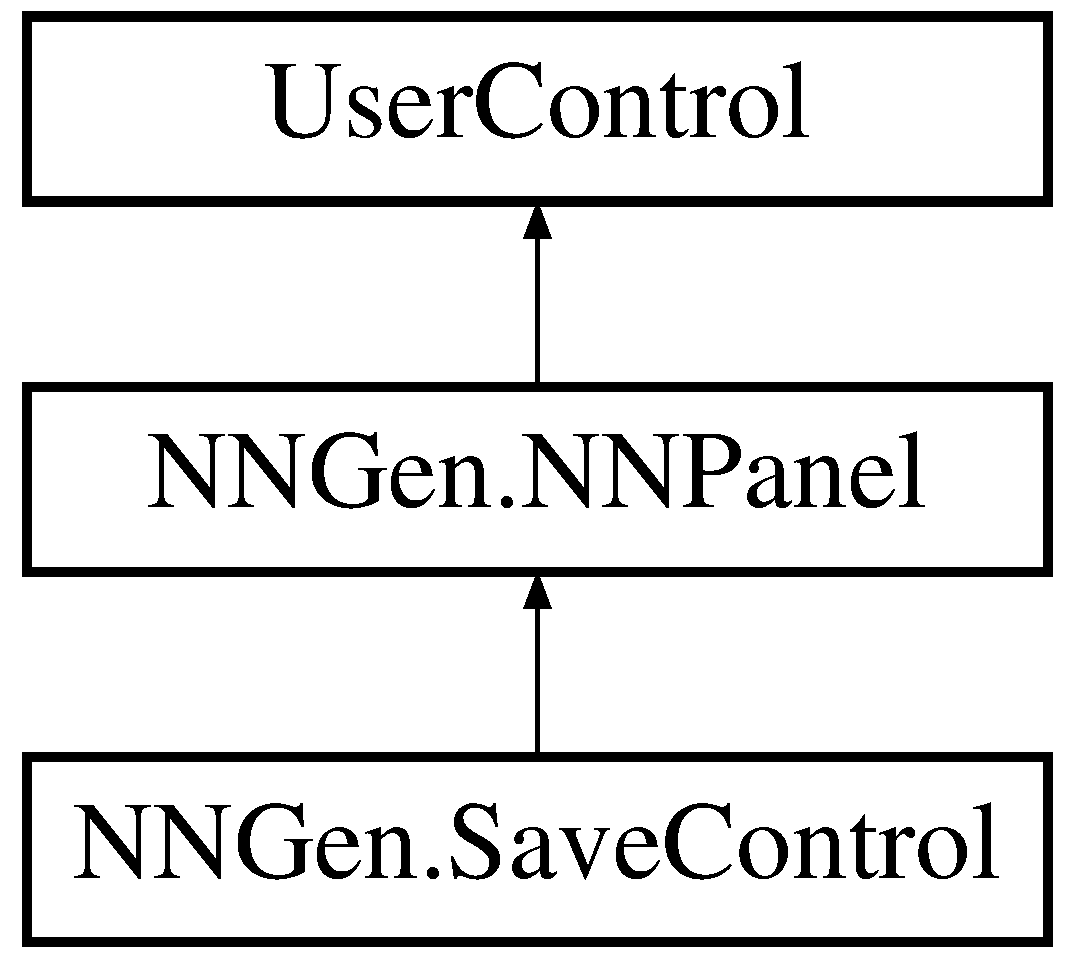
\includegraphics[height=3.000000cm]{class_n_n_gen_1_1_save_control}
\end{center}
\end{figure}
\subsection*{Public Member Functions}
\begin{DoxyCompactItemize}
\item 
\hyperlink{class_n_n_gen_1_1_save_control_affccf4dd0d6bb71a158c12f5be37d8dd}{Save\+Control} (string \+\_\+file\+Path, bool \+\_\+valid)
\begin{DoxyCompactList}\small\item\em Create a new \hyperlink{class_n_n_gen_1_1_save_control}{Save\+Control} panel \end{DoxyCompactList}\item 
override bool \hyperlink{class_n_n_gen_1_1_save_control_a9802bdb470edb0fbc0fe3d7b04863f6c}{verify} ()
\begin{DoxyCompactList}\small\item\em The \hyperlink{class_n_n_gen_1_1_save_control_a9802bdb470edb0fbc0fe3d7b04863f6c}{verify()} method implementation for this class. See N\+N\+Pannel.\+verify() for more documentation. \end{DoxyCompactList}\end{DoxyCompactItemize}
\subsection*{Public Attributes}
\begin{DoxyCompactItemize}
\item 
bool \hyperlink{class_n_n_gen_1_1_save_control_a5fd0da9af116b678a881f5ceb5ec0c40}{valid\+File\+Selected} = false
\begin{DoxyCompactList}\small\item\em A flag to determine if a valid file location has been selected \end{DoxyCompactList}\end{DoxyCompactItemize}
\subsection*{Protected Member Functions}
\begin{DoxyCompactItemize}
\item 
override void \hyperlink{class_n_n_gen_1_1_save_control_ad016d367b5079663a8bd45691391a77e}{Dispose} (bool disposing)
\begin{DoxyCompactList}\small\item\em Clean up any resources being used. \end{DoxyCompactList}\end{DoxyCompactItemize}
\subsection*{Properties}
\begin{DoxyCompactItemize}
\item 
string \hyperlink{class_n_n_gen_1_1_save_control_ac72242b01e15f912ee7c3f58592afea9}{file\+Path}\hspace{0.3cm}{\ttfamily  \mbox{[}get\mbox{]}}
\begin{DoxyCompactList}\small\item\em The file path in which the files are to be generated \end{DoxyCompactList}\end{DoxyCompactItemize}


\subsection{Detailed Description}
A U\+I element to allow the user to determine the folder in which the generated files will be saved 



\subsection{Constructor \& Destructor Documentation}
\hypertarget{class_n_n_gen_1_1_save_control_affccf4dd0d6bb71a158c12f5be37d8dd}{}\index{N\+N\+Gen\+::\+Save\+Control@{N\+N\+Gen\+::\+Save\+Control}!Save\+Control@{Save\+Control}}
\index{Save\+Control@{Save\+Control}!N\+N\+Gen\+::\+Save\+Control@{N\+N\+Gen\+::\+Save\+Control}}
\subsubsection[{Save\+Control(string \+\_\+file\+Path, bool \+\_\+valid)}]{\setlength{\rightskip}{0pt plus 5cm}N\+N\+Gen.\+Save\+Control.\+Save\+Control (
\begin{DoxyParamCaption}
\item[{string}]{\+\_\+file\+Path, }
\item[{bool}]{\+\_\+valid}
\end{DoxyParamCaption}
)\hspace{0.3cm}{\ttfamily [inline]}}\label{class_n_n_gen_1_1_save_control_affccf4dd0d6bb71a158c12f5be37d8dd}


Create a new \hyperlink{class_n_n_gen_1_1_save_control}{Save\+Control} panel 


\begin{DoxyParams}{Parameters}
{\em \+\_\+file\+Path} & The seed value for the file\+Path\\
\hline
{\em \+\_\+valid} & The seed value for whether the file\+Path is valid\\
\hline
\end{DoxyParams}


\subsection{Member Function Documentation}
\hypertarget{class_n_n_gen_1_1_save_control_ad016d367b5079663a8bd45691391a77e}{}\index{N\+N\+Gen\+::\+Save\+Control@{N\+N\+Gen\+::\+Save\+Control}!Dispose@{Dispose}}
\index{Dispose@{Dispose}!N\+N\+Gen\+::\+Save\+Control@{N\+N\+Gen\+::\+Save\+Control}}
\subsubsection[{Dispose(bool disposing)}]{\setlength{\rightskip}{0pt plus 5cm}override void N\+N\+Gen.\+Save\+Control.\+Dispose (
\begin{DoxyParamCaption}
\item[{bool}]{disposing}
\end{DoxyParamCaption}
)\hspace{0.3cm}{\ttfamily [inline]}, {\ttfamily [protected]}}\label{class_n_n_gen_1_1_save_control_ad016d367b5079663a8bd45691391a77e}


Clean up any resources being used. 


\begin{DoxyParams}{Parameters}
{\em disposing} & true if managed resources should be disposed; otherwise, false.\\
\hline
\end{DoxyParams}
\hypertarget{class_n_n_gen_1_1_save_control_a9802bdb470edb0fbc0fe3d7b04863f6c}{}\index{N\+N\+Gen\+::\+Save\+Control@{N\+N\+Gen\+::\+Save\+Control}!verify@{verify}}
\index{verify@{verify}!N\+N\+Gen\+::\+Save\+Control@{N\+N\+Gen\+::\+Save\+Control}}
\subsubsection[{verify()}]{\setlength{\rightskip}{0pt plus 5cm}override bool N\+N\+Gen.\+Save\+Control.\+verify (
\begin{DoxyParamCaption}
{}
\end{DoxyParamCaption}
)\hspace{0.3cm}{\ttfamily [inline]}, {\ttfamily [virtual]}}\label{class_n_n_gen_1_1_save_control_a9802bdb470edb0fbc0fe3d7b04863f6c}


The \hyperlink{class_n_n_gen_1_1_save_control_a9802bdb470edb0fbc0fe3d7b04863f6c}{verify()} method implementation for this class. See N\+N\+Pannel.\+verify() for more documentation. 

\begin{DoxyReturn}{Returns}

\end{DoxyReturn}


Reimplemented from \hyperlink{class_n_n_gen_1_1_n_n_panel_a36e3bcf90c9e561e8502eac6f884582a}{N\+N\+Gen.\+N\+N\+Panel}.



\subsection{Member Data Documentation}
\hypertarget{class_n_n_gen_1_1_save_control_a5fd0da9af116b678a881f5ceb5ec0c40}{}\index{N\+N\+Gen\+::\+Save\+Control@{N\+N\+Gen\+::\+Save\+Control}!valid\+File\+Selected@{valid\+File\+Selected}}
\index{valid\+File\+Selected@{valid\+File\+Selected}!N\+N\+Gen\+::\+Save\+Control@{N\+N\+Gen\+::\+Save\+Control}}
\subsubsection[{valid\+File\+Selected}]{\setlength{\rightskip}{0pt plus 5cm}bool N\+N\+Gen.\+Save\+Control.\+valid\+File\+Selected = false}\label{class_n_n_gen_1_1_save_control_a5fd0da9af116b678a881f5ceb5ec0c40}


A flag to determine if a valid file location has been selected 



\subsection{Property Documentation}
\hypertarget{class_n_n_gen_1_1_save_control_ac72242b01e15f912ee7c3f58592afea9}{}\index{N\+N\+Gen\+::\+Save\+Control@{N\+N\+Gen\+::\+Save\+Control}!file\+Path@{file\+Path}}
\index{file\+Path@{file\+Path}!N\+N\+Gen\+::\+Save\+Control@{N\+N\+Gen\+::\+Save\+Control}}
\subsubsection[{file\+Path}]{\setlength{\rightskip}{0pt plus 5cm}string N\+N\+Gen.\+Save\+Control.\+file\+Path\hspace{0.3cm}{\ttfamily [get]}}\label{class_n_n_gen_1_1_save_control_ac72242b01e15f912ee7c3f58592afea9}


The file path in which the files are to be generated 



The documentation for this class was generated from the following files\+:\begin{DoxyCompactItemize}
\item 
E\+:/\+Documents/\+Visual Studio 2013/\+Projects/\+Neural\+Network/\+N\+N\+Gen/\hyperlink{_save_control_8cs}{Save\+Control.\+cs}\item 
E\+:/\+Documents/\+Visual Studio 2013/\+Projects/\+Neural\+Network/\+N\+N\+Gen/\hyperlink{_save_control_8_designer_8cs}{Save\+Control.\+Designer.\+cs}\end{DoxyCompactItemize}

\hypertarget{class_n_n_gen_1_1_sigmoid___poly_approx}{}\section{N\+N\+Gen.\+Sigmoid\+\_\+\+Poly\+Approx Class Reference}
\label{class_n_n_gen_1_1_sigmoid___poly_approx}\index{N\+N\+Gen.\+Sigmoid\+\_\+\+Poly\+Approx@{N\+N\+Gen.\+Sigmoid\+\_\+\+Poly\+Approx}}


A thresholding function approximating the sigmoid function 1/(1 + exp(-\/x))  


Inheritance diagram for N\+N\+Gen.\+Sigmoid\+\_\+\+Poly\+Approx\+:\begin{figure}[H]
\begin{center}
\leavevmode
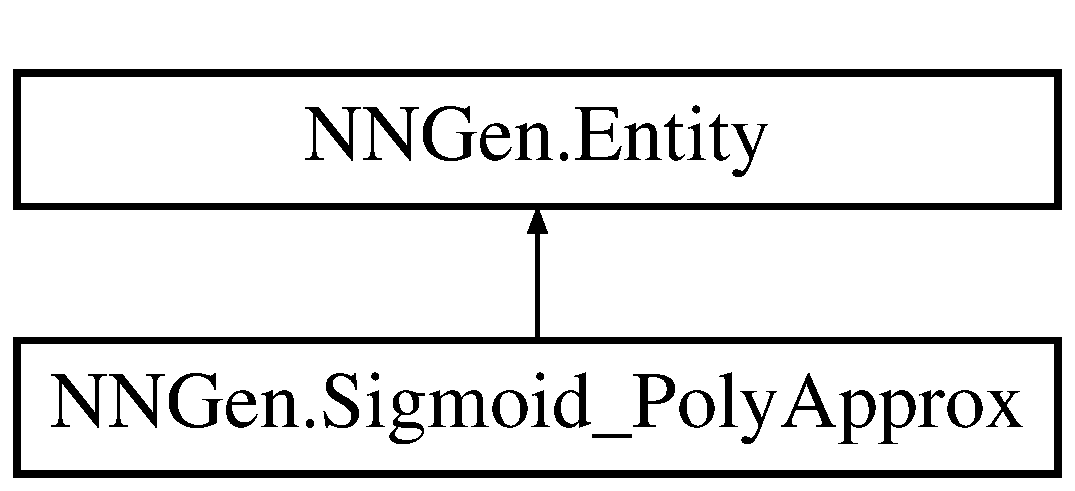
\includegraphics[height=2.000000cm]{class_n_n_gen_1_1_sigmoid___poly_approx}
\end{center}
\end{figure}
\subsection*{Public Member Functions}
\begin{DoxyCompactItemize}
\item 
\hyperlink{class_n_n_gen_1_1_sigmoid___poly_approx_afcf01b0610e4b2835f237038e7f3ff40}{Sigmoid\+\_\+\+Poly\+Approx} (\hyperlink{class_n_n_gen_1_1_port}{Port} \+\_\+sigmoid\+Input\+Port, int \+\_\+output\+Int\+Bits, int \+\_\+output\+Frac\+Bits, string \+\_\+name)
\begin{DoxyCompactList}\small\item\em Initializes the Sigmoid thresholding element \end{DoxyCompactList}\item 
\hyperlink{class_n_n_gen_1_1_sigmoid___poly_approx_a911d3d616c3eceb6ff57bfe371489264}{Sigmoid\+\_\+\+Poly\+Approx} (\hyperlink{class_n_n_gen_1_1_signal}{Signal} \+\_\+sigmoid\+Input\+Sigmal, int \+\_\+output\+Int\+Bits, int \+\_\+output\+Frac\+Bits, string \+\_\+name)
\begin{DoxyCompactList}\small\item\em Initializes the Sigmoid thresholding element \end{DoxyCompactList}\item 
override string \hyperlink{class_n_n_gen_1_1_sigmoid___poly_approx_a68e8a0e324f6cae64ee7d2f841c35506}{get\+Name} ()
\begin{DoxyCompactList}\small\item\em Returns the name of the entity \end{DoxyCompactList}\item 
override \hyperlink{class_n_n_gen_1_1_port}{Port}\mbox{[}$\,$\mbox{]} \hyperlink{class_n_n_gen_1_1_sigmoid___poly_approx_ac4cf07415c0dc69efdaf91cfc561b68f}{get\+Input\+Ports} ()
\begin{DoxyCompactList}\small\item\em Returns the input ports to the device \end{DoxyCompactList}\item 
override \hyperlink{class_n_n_gen_1_1_port}{Port}\mbox{[}$\,$\mbox{]} \hyperlink{class_n_n_gen_1_1_sigmoid___poly_approx_ad4add2a8c53cc31373dab81e8ea634e2}{get\+Output\+Ports} ()
\begin{DoxyCompactList}\small\item\em Returns the output ports to the device \end{DoxyCompactList}\item 
override \hyperlink{class_n_n_gen_1_1_signal}{Signal}\mbox{[}$\,$\mbox{]} \hyperlink{class_n_n_gen_1_1_sigmoid___poly_approx_aa9ea30f1d5fa7e2ff1874f00e37deffb}{get\+Internal\+Signals} ()
\begin{DoxyCompactList}\small\item\em Returns the internal signals of the device \end{DoxyCompactList}\item 
override bool \hyperlink{class_n_n_gen_1_1_sigmoid___poly_approx_a1d78cd23e2a1f4e686980052ad8c7a44}{write\+V\+H\+D\+L} (string file)
\begin{DoxyCompactList}\small\item\em Writes the .vhd files necessary to compile this entity. All other necessary entities (i.\+e. neurons, thresholding functions, etc.) will also be written when this function returns \end{DoxyCompactList}\end{DoxyCompactItemize}
\subsection*{Public Attributes}
\begin{DoxyCompactItemize}
\item 
string \hyperlink{class_n_n_gen_1_1_sigmoid___poly_approx_ae95905d2d05007afee1e105e93c64045}{name} = \char`\"{}sigmoid\+\_\+poly\+Approx\char`\"{}
\begin{DoxyCompactList}\small\item\em The name of the entity \end{DoxyCompactList}\end{DoxyCompactItemize}
\subsection*{Properties}
\begin{DoxyCompactItemize}
\item 
\hyperlink{class_n_n_gen_1_1_port}{Port} \hyperlink{class_n_n_gen_1_1_sigmoid___poly_approx_ae6da90acd8f62414c3ead1c2cc8538da}{sigmoid\+Input}\hspace{0.3cm}{\ttfamily  \mbox{[}get\mbox{]}}
\begin{DoxyCompactList}\small\item\em The input signal to the thresholding function \end{DoxyCompactList}\item 
\hyperlink{class_n_n_gen_1_1_port}{Port} \hyperlink{class_n_n_gen_1_1_sigmoid___poly_approx_a93bf10c040a0ed7dd4428c9df4539188}{sigmoid\+Output}\hspace{0.3cm}{\ttfamily  \mbox{[}get\mbox{]}}
\begin{DoxyCompactList}\small\item\em The output signal to the thresholding function \end{DoxyCompactList}\item 
\hyperlink{class_n_n_gen_1_1_signal}{Signal} \hyperlink{class_n_n_gen_1_1_sigmoid___poly_approx_a14047a901c8101e599e807f4ef07d46d}{numerator}\hspace{0.3cm}{\ttfamily  \mbox{[}get\mbox{]}}
\begin{DoxyCompactList}\small\item\em An internal signal used in the sigmoid computation \end{DoxyCompactList}\item 
\hyperlink{class_n_n_gen_1_1_signal}{Signal} \hyperlink{class_n_n_gen_1_1_sigmoid___poly_approx_a371e8a19a69ffabafa7f6e2819b3c5b6}{denominator}\hspace{0.3cm}{\ttfamily  \mbox{[}get\mbox{]}}
\begin{DoxyCompactList}\small\item\em An internal signal used in the sigmoid computation \end{DoxyCompactList}\item 
\hyperlink{class_n_n_gen_1_1_signal}{Signal} \hyperlink{class_n_n_gen_1_1_sigmoid___poly_approx_af795af0bd003e50d11e5f3c904d03dca}{thresh\+\_\+sum}\hspace{0.3cm}{\ttfamily  \mbox{[}get\mbox{]}}
\begin{DoxyCompactList}\small\item\em An internal signal used in the sigmoid computation \end{DoxyCompactList}\item 
int \hyperlink{class_n_n_gen_1_1_sigmoid___poly_approx_a3834aa67d528e6f7b4698d651a28d027}{output\+Frac\+Bits}\hspace{0.3cm}{\ttfamily  \mbox{[}get\mbox{]}}
\begin{DoxyCompactList}\small\item\em The number of bits to use in the output signal representing the fractional portion of the result \end{DoxyCompactList}\item 
int \hyperlink{class_n_n_gen_1_1_sigmoid___poly_approx_ad9f06e6995afc2b5f049c4d062e6b716}{output\+Int\+Bits}\hspace{0.3cm}{\ttfamily  \mbox{[}get\mbox{]}}
\begin{DoxyCompactList}\small\item\em The number of integer bits to use in the output signal. These will all be zeros, but this member can be useful to merge signal sizes \end{DoxyCompactList}\end{DoxyCompactItemize}


\subsection{Detailed Description}
A thresholding function approximating the sigmoid function 1/(1 + exp(-\/x)) 

This class uses the approximation sigmoid(x) $\sim$ (1/2) $\ast$ ( 1 + (x/(x+1)) ) 

\subsection{Constructor \& Destructor Documentation}
\hypertarget{class_n_n_gen_1_1_sigmoid___poly_approx_afcf01b0610e4b2835f237038e7f3ff40}{}\index{N\+N\+Gen\+::\+Sigmoid\+\_\+\+Poly\+Approx@{N\+N\+Gen\+::\+Sigmoid\+\_\+\+Poly\+Approx}!Sigmoid\+\_\+\+Poly\+Approx@{Sigmoid\+\_\+\+Poly\+Approx}}
\index{Sigmoid\+\_\+\+Poly\+Approx@{Sigmoid\+\_\+\+Poly\+Approx}!N\+N\+Gen\+::\+Sigmoid\+\_\+\+Poly\+Approx@{N\+N\+Gen\+::\+Sigmoid\+\_\+\+Poly\+Approx}}
\subsubsection[{Sigmoid\+\_\+\+Poly\+Approx(\+Port \+\_\+sigmoid\+Input\+Port, int \+\_\+output\+Int\+Bits, int \+\_\+output\+Frac\+Bits, string \+\_\+name)}]{\setlength{\rightskip}{0pt plus 5cm}N\+N\+Gen.\+Sigmoid\+\_\+\+Poly\+Approx.\+Sigmoid\+\_\+\+Poly\+Approx (
\begin{DoxyParamCaption}
\item[{{\bf Port}}]{\+\_\+sigmoid\+Input\+Port, }
\item[{int}]{\+\_\+output\+Int\+Bits, }
\item[{int}]{\+\_\+output\+Frac\+Bits, }
\item[{string}]{\+\_\+name}
\end{DoxyParamCaption}
)\hspace{0.3cm}{\ttfamily [inline]}}\label{class_n_n_gen_1_1_sigmoid___poly_approx_afcf01b0610e4b2835f237038e7f3ff40}


Initializes the Sigmoid thresholding element 


\begin{DoxyParams}{Parameters}
{\em \+\_\+sigmoid\+Input\+Port} & The input port to the device\\
\hline
{\em \+\_\+output\+Int\+Bits} & The number of integer bits to be used in the output. These will all be zeroes, but this can be useful in matching bus widths in higher level entities\\
\hline
{\em \+\_\+output\+Frac\+Bits} & The number of fractional bits to be used in the output.\\
\hline
{\em \+\_\+name} & The name of the entity\\
\hline
\end{DoxyParams}
\hypertarget{class_n_n_gen_1_1_sigmoid___poly_approx_a911d3d616c3eceb6ff57bfe371489264}{}\index{N\+N\+Gen\+::\+Sigmoid\+\_\+\+Poly\+Approx@{N\+N\+Gen\+::\+Sigmoid\+\_\+\+Poly\+Approx}!Sigmoid\+\_\+\+Poly\+Approx@{Sigmoid\+\_\+\+Poly\+Approx}}
\index{Sigmoid\+\_\+\+Poly\+Approx@{Sigmoid\+\_\+\+Poly\+Approx}!N\+N\+Gen\+::\+Sigmoid\+\_\+\+Poly\+Approx@{N\+N\+Gen\+::\+Sigmoid\+\_\+\+Poly\+Approx}}
\subsubsection[{Sigmoid\+\_\+\+Poly\+Approx(\+Signal \+\_\+sigmoid\+Input\+Sigmal, int \+\_\+output\+Int\+Bits, int \+\_\+output\+Frac\+Bits, string \+\_\+name)}]{\setlength{\rightskip}{0pt plus 5cm}N\+N\+Gen.\+Sigmoid\+\_\+\+Poly\+Approx.\+Sigmoid\+\_\+\+Poly\+Approx (
\begin{DoxyParamCaption}
\item[{{\bf Signal}}]{\+\_\+sigmoid\+Input\+Sigmal, }
\item[{int}]{\+\_\+output\+Int\+Bits, }
\item[{int}]{\+\_\+output\+Frac\+Bits, }
\item[{string}]{\+\_\+name}
\end{DoxyParamCaption}
)\hspace{0.3cm}{\ttfamily [inline]}}\label{class_n_n_gen_1_1_sigmoid___poly_approx_a911d3d616c3eceb6ff57bfe371489264}


Initializes the Sigmoid thresholding element 


\begin{DoxyParams}{Parameters}
{\em \+\_\+sigmoid\+Input\+Sigmal} & The input signal to the device\\
\hline
{\em \+\_\+output\+Int\+Bits} & The number of integer bits to be used in the output. These will all be zeroes, but this can be useful in matching bus widths in higher level entities\\
\hline
{\em \+\_\+output\+Frac\+Bits} & The number of fractional bits to be used in the output.\\
\hline
{\em \+\_\+name} & The name of the entity\\
\hline
\end{DoxyParams}


\subsection{Member Function Documentation}
\hypertarget{class_n_n_gen_1_1_sigmoid___poly_approx_ac4cf07415c0dc69efdaf91cfc561b68f}{}\index{N\+N\+Gen\+::\+Sigmoid\+\_\+\+Poly\+Approx@{N\+N\+Gen\+::\+Sigmoid\+\_\+\+Poly\+Approx}!get\+Input\+Ports@{get\+Input\+Ports}}
\index{get\+Input\+Ports@{get\+Input\+Ports}!N\+N\+Gen\+::\+Sigmoid\+\_\+\+Poly\+Approx@{N\+N\+Gen\+::\+Sigmoid\+\_\+\+Poly\+Approx}}
\subsubsection[{get\+Input\+Ports()}]{\setlength{\rightskip}{0pt plus 5cm}override {\bf Port} \mbox{[}$\,$\mbox{]} N\+N\+Gen.\+Sigmoid\+\_\+\+Poly\+Approx.\+get\+Input\+Ports (
\begin{DoxyParamCaption}
{}
\end{DoxyParamCaption}
)\hspace{0.3cm}{\ttfamily [inline]}, {\ttfamily [virtual]}}\label{class_n_n_gen_1_1_sigmoid___poly_approx_ac4cf07415c0dc69efdaf91cfc561b68f}


Returns the input ports to the device 

\begin{DoxyReturn}{Returns}
The input ports to the device
\end{DoxyReturn}


Implements \hyperlink{class_n_n_gen_1_1_entity_a01239f05c9efa61ec9e6a29cb2eaad50}{N\+N\+Gen.\+Entity}.

\hypertarget{class_n_n_gen_1_1_sigmoid___poly_approx_aa9ea30f1d5fa7e2ff1874f00e37deffb}{}\index{N\+N\+Gen\+::\+Sigmoid\+\_\+\+Poly\+Approx@{N\+N\+Gen\+::\+Sigmoid\+\_\+\+Poly\+Approx}!get\+Internal\+Signals@{get\+Internal\+Signals}}
\index{get\+Internal\+Signals@{get\+Internal\+Signals}!N\+N\+Gen\+::\+Sigmoid\+\_\+\+Poly\+Approx@{N\+N\+Gen\+::\+Sigmoid\+\_\+\+Poly\+Approx}}
\subsubsection[{get\+Internal\+Signals()}]{\setlength{\rightskip}{0pt plus 5cm}override {\bf Signal} \mbox{[}$\,$\mbox{]} N\+N\+Gen.\+Sigmoid\+\_\+\+Poly\+Approx.\+get\+Internal\+Signals (
\begin{DoxyParamCaption}
{}
\end{DoxyParamCaption}
)\hspace{0.3cm}{\ttfamily [inline]}, {\ttfamily [virtual]}}\label{class_n_n_gen_1_1_sigmoid___poly_approx_aa9ea30f1d5fa7e2ff1874f00e37deffb}


Returns the internal signals of the device 

\begin{DoxyReturn}{Returns}
The internal signals of the device
\end{DoxyReturn}


Implements \hyperlink{class_n_n_gen_1_1_entity_a62feb80e95ec84c650ea17bd53f0d510}{N\+N\+Gen.\+Entity}.

\hypertarget{class_n_n_gen_1_1_sigmoid___poly_approx_a68e8a0e324f6cae64ee7d2f841c35506}{}\index{N\+N\+Gen\+::\+Sigmoid\+\_\+\+Poly\+Approx@{N\+N\+Gen\+::\+Sigmoid\+\_\+\+Poly\+Approx}!get\+Name@{get\+Name}}
\index{get\+Name@{get\+Name}!N\+N\+Gen\+::\+Sigmoid\+\_\+\+Poly\+Approx@{N\+N\+Gen\+::\+Sigmoid\+\_\+\+Poly\+Approx}}
\subsubsection[{get\+Name()}]{\setlength{\rightskip}{0pt plus 5cm}override string N\+N\+Gen.\+Sigmoid\+\_\+\+Poly\+Approx.\+get\+Name (
\begin{DoxyParamCaption}
{}
\end{DoxyParamCaption}
)\hspace{0.3cm}{\ttfamily [inline]}, {\ttfamily [virtual]}}\label{class_n_n_gen_1_1_sigmoid___poly_approx_a68e8a0e324f6cae64ee7d2f841c35506}


Returns the name of the entity 

\begin{DoxyReturn}{Returns}
The name of the entity
\end{DoxyReturn}


Implements \hyperlink{class_n_n_gen_1_1_entity_a9f25d1070c9ab8ad343c28443e62e6f2}{N\+N\+Gen.\+Entity}.

\hypertarget{class_n_n_gen_1_1_sigmoid___poly_approx_ad4add2a8c53cc31373dab81e8ea634e2}{}\index{N\+N\+Gen\+::\+Sigmoid\+\_\+\+Poly\+Approx@{N\+N\+Gen\+::\+Sigmoid\+\_\+\+Poly\+Approx}!get\+Output\+Ports@{get\+Output\+Ports}}
\index{get\+Output\+Ports@{get\+Output\+Ports}!N\+N\+Gen\+::\+Sigmoid\+\_\+\+Poly\+Approx@{N\+N\+Gen\+::\+Sigmoid\+\_\+\+Poly\+Approx}}
\subsubsection[{get\+Output\+Ports()}]{\setlength{\rightskip}{0pt plus 5cm}override {\bf Port} \mbox{[}$\,$\mbox{]} N\+N\+Gen.\+Sigmoid\+\_\+\+Poly\+Approx.\+get\+Output\+Ports (
\begin{DoxyParamCaption}
{}
\end{DoxyParamCaption}
)\hspace{0.3cm}{\ttfamily [inline]}, {\ttfamily [virtual]}}\label{class_n_n_gen_1_1_sigmoid___poly_approx_ad4add2a8c53cc31373dab81e8ea634e2}


Returns the output ports to the device 

\begin{DoxyReturn}{Returns}
The output ports of the device
\end{DoxyReturn}


Implements \hyperlink{class_n_n_gen_1_1_entity_ace06368087778e254a5048c7d28747be}{N\+N\+Gen.\+Entity}.

\hypertarget{class_n_n_gen_1_1_sigmoid___poly_approx_a1d78cd23e2a1f4e686980052ad8c7a44}{}\index{N\+N\+Gen\+::\+Sigmoid\+\_\+\+Poly\+Approx@{N\+N\+Gen\+::\+Sigmoid\+\_\+\+Poly\+Approx}!write\+V\+H\+D\+L@{write\+V\+H\+D\+L}}
\index{write\+V\+H\+D\+L@{write\+V\+H\+D\+L}!N\+N\+Gen\+::\+Sigmoid\+\_\+\+Poly\+Approx@{N\+N\+Gen\+::\+Sigmoid\+\_\+\+Poly\+Approx}}
\subsubsection[{write\+V\+H\+D\+L(string file)}]{\setlength{\rightskip}{0pt plus 5cm}override bool N\+N\+Gen.\+Sigmoid\+\_\+\+Poly\+Approx.\+write\+V\+H\+D\+L (
\begin{DoxyParamCaption}
\item[{string}]{file}
\end{DoxyParamCaption}
)\hspace{0.3cm}{\ttfamily [inline]}, {\ttfamily [virtual]}}\label{class_n_n_gen_1_1_sigmoid___poly_approx_a1d78cd23e2a1f4e686980052ad8c7a44}


Writes the .vhd files necessary to compile this entity. All other necessary entities (i.\+e. neurons, thresholding functions, etc.) will also be written when this function returns 


\begin{DoxyParams}{Parameters}
{\em file} & The file path in which to write the files (do N\+O\+T include \char`\"{}...\+name.\+vhd\char`\"{}\\
\hline
\end{DoxyParams}
\begin{DoxyReturn}{Returns}
true if the files were written successfully, false otherwise
\end{DoxyReturn}


Implements \hyperlink{class_n_n_gen_1_1_entity_a1111d498446be08b20583b9625893a52}{N\+N\+Gen.\+Entity}.



\subsection{Member Data Documentation}
\hypertarget{class_n_n_gen_1_1_sigmoid___poly_approx_ae95905d2d05007afee1e105e93c64045}{}\index{N\+N\+Gen\+::\+Sigmoid\+\_\+\+Poly\+Approx@{N\+N\+Gen\+::\+Sigmoid\+\_\+\+Poly\+Approx}!name@{name}}
\index{name@{name}!N\+N\+Gen\+::\+Sigmoid\+\_\+\+Poly\+Approx@{N\+N\+Gen\+::\+Sigmoid\+\_\+\+Poly\+Approx}}
\subsubsection[{name}]{\setlength{\rightskip}{0pt plus 5cm}string N\+N\+Gen.\+Sigmoid\+\_\+\+Poly\+Approx.\+name = \char`\"{}sigmoid\+\_\+poly\+Approx\char`\"{}}\label{class_n_n_gen_1_1_sigmoid___poly_approx_ae95905d2d05007afee1e105e93c64045}


The name of the entity 



\subsection{Property Documentation}
\hypertarget{class_n_n_gen_1_1_sigmoid___poly_approx_a371e8a19a69ffabafa7f6e2819b3c5b6}{}\index{N\+N\+Gen\+::\+Sigmoid\+\_\+\+Poly\+Approx@{N\+N\+Gen\+::\+Sigmoid\+\_\+\+Poly\+Approx}!denominator@{denominator}}
\index{denominator@{denominator}!N\+N\+Gen\+::\+Sigmoid\+\_\+\+Poly\+Approx@{N\+N\+Gen\+::\+Sigmoid\+\_\+\+Poly\+Approx}}
\subsubsection[{denominator}]{\setlength{\rightskip}{0pt plus 5cm}{\bf Signal} N\+N\+Gen.\+Sigmoid\+\_\+\+Poly\+Approx.\+denominator\hspace{0.3cm}{\ttfamily [get]}}\label{class_n_n_gen_1_1_sigmoid___poly_approx_a371e8a19a69ffabafa7f6e2819b3c5b6}


An internal signal used in the sigmoid computation 

\hypertarget{class_n_n_gen_1_1_sigmoid___poly_approx_a14047a901c8101e599e807f4ef07d46d}{}\index{N\+N\+Gen\+::\+Sigmoid\+\_\+\+Poly\+Approx@{N\+N\+Gen\+::\+Sigmoid\+\_\+\+Poly\+Approx}!numerator@{numerator}}
\index{numerator@{numerator}!N\+N\+Gen\+::\+Sigmoid\+\_\+\+Poly\+Approx@{N\+N\+Gen\+::\+Sigmoid\+\_\+\+Poly\+Approx}}
\subsubsection[{numerator}]{\setlength{\rightskip}{0pt plus 5cm}{\bf Signal} N\+N\+Gen.\+Sigmoid\+\_\+\+Poly\+Approx.\+numerator\hspace{0.3cm}{\ttfamily [get]}}\label{class_n_n_gen_1_1_sigmoid___poly_approx_a14047a901c8101e599e807f4ef07d46d}


An internal signal used in the sigmoid computation 

\hypertarget{class_n_n_gen_1_1_sigmoid___poly_approx_a3834aa67d528e6f7b4698d651a28d027}{}\index{N\+N\+Gen\+::\+Sigmoid\+\_\+\+Poly\+Approx@{N\+N\+Gen\+::\+Sigmoid\+\_\+\+Poly\+Approx}!output\+Frac\+Bits@{output\+Frac\+Bits}}
\index{output\+Frac\+Bits@{output\+Frac\+Bits}!N\+N\+Gen\+::\+Sigmoid\+\_\+\+Poly\+Approx@{N\+N\+Gen\+::\+Sigmoid\+\_\+\+Poly\+Approx}}
\subsubsection[{output\+Frac\+Bits}]{\setlength{\rightskip}{0pt plus 5cm}int N\+N\+Gen.\+Sigmoid\+\_\+\+Poly\+Approx.\+output\+Frac\+Bits\hspace{0.3cm}{\ttfamily [get]}}\label{class_n_n_gen_1_1_sigmoid___poly_approx_a3834aa67d528e6f7b4698d651a28d027}


The number of bits to use in the output signal representing the fractional portion of the result 

\hypertarget{class_n_n_gen_1_1_sigmoid___poly_approx_ad9f06e6995afc2b5f049c4d062e6b716}{}\index{N\+N\+Gen\+::\+Sigmoid\+\_\+\+Poly\+Approx@{N\+N\+Gen\+::\+Sigmoid\+\_\+\+Poly\+Approx}!output\+Int\+Bits@{output\+Int\+Bits}}
\index{output\+Int\+Bits@{output\+Int\+Bits}!N\+N\+Gen\+::\+Sigmoid\+\_\+\+Poly\+Approx@{N\+N\+Gen\+::\+Sigmoid\+\_\+\+Poly\+Approx}}
\subsubsection[{output\+Int\+Bits}]{\setlength{\rightskip}{0pt plus 5cm}int N\+N\+Gen.\+Sigmoid\+\_\+\+Poly\+Approx.\+output\+Int\+Bits\hspace{0.3cm}{\ttfamily [get]}}\label{class_n_n_gen_1_1_sigmoid___poly_approx_ad9f06e6995afc2b5f049c4d062e6b716}


The number of integer bits to use in the output signal. These will all be zeros, but this member can be useful to merge signal sizes 

\hypertarget{class_n_n_gen_1_1_sigmoid___poly_approx_ae6da90acd8f62414c3ead1c2cc8538da}{}\index{N\+N\+Gen\+::\+Sigmoid\+\_\+\+Poly\+Approx@{N\+N\+Gen\+::\+Sigmoid\+\_\+\+Poly\+Approx}!sigmoid\+Input@{sigmoid\+Input}}
\index{sigmoid\+Input@{sigmoid\+Input}!N\+N\+Gen\+::\+Sigmoid\+\_\+\+Poly\+Approx@{N\+N\+Gen\+::\+Sigmoid\+\_\+\+Poly\+Approx}}
\subsubsection[{sigmoid\+Input}]{\setlength{\rightskip}{0pt plus 5cm}{\bf Port} N\+N\+Gen.\+Sigmoid\+\_\+\+Poly\+Approx.\+sigmoid\+Input\hspace{0.3cm}{\ttfamily [get]}}\label{class_n_n_gen_1_1_sigmoid___poly_approx_ae6da90acd8f62414c3ead1c2cc8538da}


The input signal to the thresholding function 

\hypertarget{class_n_n_gen_1_1_sigmoid___poly_approx_a93bf10c040a0ed7dd4428c9df4539188}{}\index{N\+N\+Gen\+::\+Sigmoid\+\_\+\+Poly\+Approx@{N\+N\+Gen\+::\+Sigmoid\+\_\+\+Poly\+Approx}!sigmoid\+Output@{sigmoid\+Output}}
\index{sigmoid\+Output@{sigmoid\+Output}!N\+N\+Gen\+::\+Sigmoid\+\_\+\+Poly\+Approx@{N\+N\+Gen\+::\+Sigmoid\+\_\+\+Poly\+Approx}}
\subsubsection[{sigmoid\+Output}]{\setlength{\rightskip}{0pt plus 5cm}{\bf Port} N\+N\+Gen.\+Sigmoid\+\_\+\+Poly\+Approx.\+sigmoid\+Output\hspace{0.3cm}{\ttfamily [get]}}\label{class_n_n_gen_1_1_sigmoid___poly_approx_a93bf10c040a0ed7dd4428c9df4539188}


The output signal to the thresholding function 

\hypertarget{class_n_n_gen_1_1_sigmoid___poly_approx_af795af0bd003e50d11e5f3c904d03dca}{}\index{N\+N\+Gen\+::\+Sigmoid\+\_\+\+Poly\+Approx@{N\+N\+Gen\+::\+Sigmoid\+\_\+\+Poly\+Approx}!thresh\+\_\+sum@{thresh\+\_\+sum}}
\index{thresh\+\_\+sum@{thresh\+\_\+sum}!N\+N\+Gen\+::\+Sigmoid\+\_\+\+Poly\+Approx@{N\+N\+Gen\+::\+Sigmoid\+\_\+\+Poly\+Approx}}
\subsubsection[{thresh\+\_\+sum}]{\setlength{\rightskip}{0pt plus 5cm}{\bf Signal} N\+N\+Gen.\+Sigmoid\+\_\+\+Poly\+Approx.\+thresh\+\_\+sum\hspace{0.3cm}{\ttfamily [get]}}\label{class_n_n_gen_1_1_sigmoid___poly_approx_af795af0bd003e50d11e5f3c904d03dca}


An internal signal used in the sigmoid computation 



The documentation for this class was generated from the following file\+:\begin{DoxyCompactItemize}
\item 
E\+:/\+Documents/\+Visual Studio 2013/\+Projects/\+Neural\+Network/\+N\+N\+Gen/\hyperlink{sigmoid__poly_approx_8cs}{sigmoid\+\_\+poly\+Approx.\+cs}\end{DoxyCompactItemize}

\hypertarget{class_n_n_gen_1_1_signal}{}\section{N\+N\+Gen.\+Signal Class Reference}
\label{class_n_n_gen_1_1_signal}\index{N\+N\+Gen.\+Signal@{N\+N\+Gen.\+Signal}}


A class representing an internal signal for a V\+H\+D\+L entity  


Inheritance diagram for N\+N\+Gen.\+Signal\+:\begin{figure}[H]
\begin{center}
\leavevmode
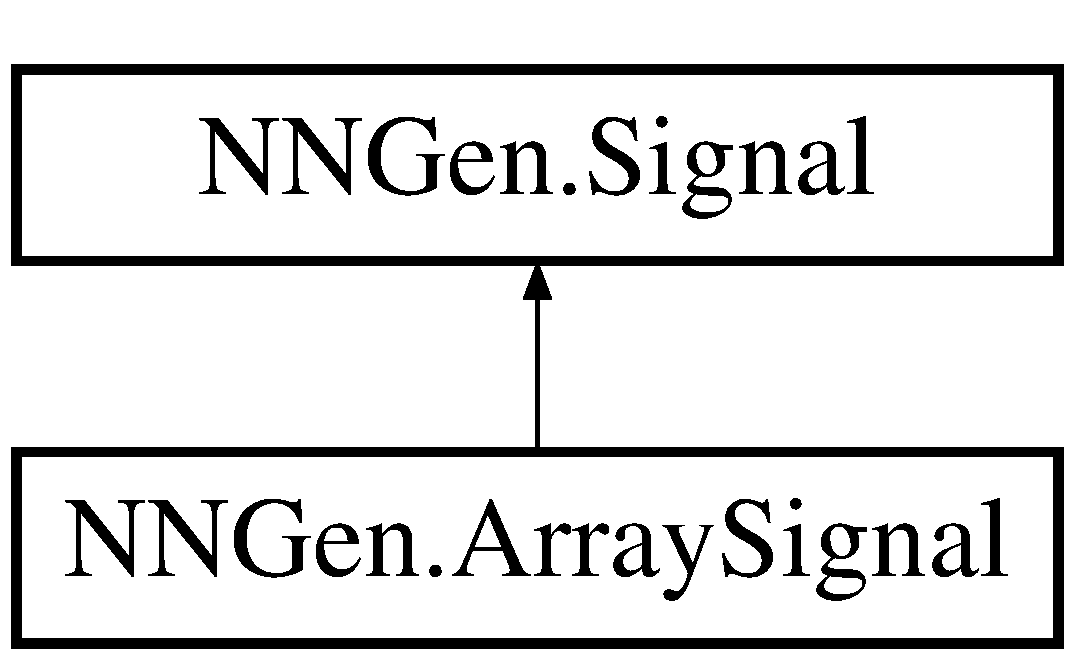
\includegraphics[height=2.000000cm]{class_n_n_gen_1_1_signal}
\end{center}
\end{figure}
\subsection*{Public Member Functions}
\begin{DoxyCompactItemize}
\item 
\hyperlink{class_n_n_gen_1_1_signal_a8e17b61cd22e4d1492b42f93f0f066f9}{Signal} (string \+\_\+name, Utilities.\+V\+H\+D\+L\+Data\+Type \+\_\+type, string \+\_\+default\+Value, int \+\_\+top, int \+\_\+bottom)
\begin{DoxyCompactList}\small\item\em Initializes a signal \end{DoxyCompactList}\item 
virtual string \hyperlink{class_n_n_gen_1_1_signal_a35818f3d3a0c4c567701300d90c846ff}{V\+H\+D\+L\+String} ()
\begin{DoxyCompactList}\small\item\em Returns a string declaring the signal \end{DoxyCompactList}\item 
virtual \hyperlink{class_n_n_gen_1_1_port}{Port} \hyperlink{class_n_n_gen_1_1_signal_a15f668236a819dab4054232fc8e82895}{to\+Port} (\hyperlink{class_n_n_gen_1_1_port_ac3b8f11a7a6bd6872e6954b64721d90c}{Port.\+port\+Direction} \+\_\+dir)
\begin{DoxyCompactList}\small\item\em Returns a port with the same parameters of the signal \end{DoxyCompactList}\end{DoxyCompactItemize}
\subsection*{Properties}
\begin{DoxyCompactItemize}
\item 
string \hyperlink{class_n_n_gen_1_1_signal_ae7a3bd5d6385e96cbd244dfdf674a6e6}{name}\hspace{0.3cm}{\ttfamily  \mbox{[}get\mbox{]}}
\begin{DoxyCompactList}\small\item\em The name of the signal \end{DoxyCompactList}\item 
Utilities.\+V\+H\+D\+L\+Data\+Type \hyperlink{class_n_n_gen_1_1_signal_a587998f4c25cb8bdaf5358e9f240c122}{type}\hspace{0.3cm}{\ttfamily  \mbox{[}get\mbox{]}}
\begin{DoxyCompactList}\small\item\em The datatype of the signal \end{DoxyCompactList}\item 
string \hyperlink{class_n_n_gen_1_1_signal_ac98333aa2ce1fdd3f3748ba8cfc4b932}{default\+Value}\hspace{0.3cm}{\ttfamily  \mbox{[}get\mbox{]}}
\begin{DoxyCompactList}\small\item\em The default value of the signal. If not specified, then it will be null \end{DoxyCompactList}\item 
int \hyperlink{class_n_n_gen_1_1_signal_a0ba4a498e3bc647b39a2c100c7d8cd60}{top}\hspace{0.3cm}{\ttfamily  \mbox{[}get\mbox{]}}
\begin{DoxyCompactList}\small\item\em The top integer in the bus width declaration (i.\+e. the \textquotesingle{}X\textquotesingle{} in (X D\+O\+W\+N\+T\+O Y)) \end{DoxyCompactList}\item 
int \hyperlink{class_n_n_gen_1_1_signal_a62c486db61e28bb2348c2534f25780cc}{bottom}\hspace{0.3cm}{\ttfamily  \mbox{[}get\mbox{]}}
\begin{DoxyCompactList}\small\item\em The bottom integer in the bus width declaration (i.\+e. the \textquotesingle{}Y\textquotesingle{} in (X D\+O\+W\+N\+T\+O Y)) \end{DoxyCompactList}\end{DoxyCompactItemize}


\subsection{Detailed Description}
A class representing an internal signal for a V\+H\+D\+L entity 



\subsection{Constructor \& Destructor Documentation}
\hypertarget{class_n_n_gen_1_1_signal_a8e17b61cd22e4d1492b42f93f0f066f9}{}\index{N\+N\+Gen\+::\+Signal@{N\+N\+Gen\+::\+Signal}!Signal@{Signal}}
\index{Signal@{Signal}!N\+N\+Gen\+::\+Signal@{N\+N\+Gen\+::\+Signal}}
\subsubsection[{Signal(string \+\_\+name, Utilities.\+V\+H\+D\+L\+Data\+Type \+\_\+type, string \+\_\+default\+Value, int \+\_\+top, int \+\_\+bottom)}]{\setlength{\rightskip}{0pt plus 5cm}N\+N\+Gen.\+Signal.\+Signal (
\begin{DoxyParamCaption}
\item[{string}]{\+\_\+name, }
\item[{Utilities.\+V\+H\+D\+L\+Data\+Type}]{\+\_\+type, }
\item[{string}]{\+\_\+default\+Value, }
\item[{int}]{\+\_\+top, }
\item[{int}]{\+\_\+bottom}
\end{DoxyParamCaption}
)\hspace{0.3cm}{\ttfamily [inline]}}\label{class_n_n_gen_1_1_signal_a8e17b61cd22e4d1492b42f93f0f066f9}


Initializes a signal 


\begin{DoxyParams}{Parameters}
{\em \+\_\+name} & The name of the signal\\
\hline
{\em \+\_\+type} & The datatype of the signal\\
\hline
{\em \+\_\+default\+Value} & The default value for the signal. If not specified, pass \textquotesingle{}null\textquotesingle{}\\
\hline
{\em \+\_\+top} & The top integer in the bus width declaration (i.\+e. the \textquotesingle{}X\textquotesingle{} in (X D\+O\+W\+N\+T\+O Y))\\
\hline
{\em \+\_\+bottom} & The bottom integer in the bus width declaration (i.\+e. the \textquotesingle{}Y\textquotesingle{} in (X D\+O\+W\+N\+T\+O Y))\\
\hline
\end{DoxyParams}


\subsection{Member Function Documentation}
\hypertarget{class_n_n_gen_1_1_signal_a15f668236a819dab4054232fc8e82895}{}\index{N\+N\+Gen\+::\+Signal@{N\+N\+Gen\+::\+Signal}!to\+Port@{to\+Port}}
\index{to\+Port@{to\+Port}!N\+N\+Gen\+::\+Signal@{N\+N\+Gen\+::\+Signal}}
\subsubsection[{to\+Port(\+Port.\+port\+Direction \+\_\+dir)}]{\setlength{\rightskip}{0pt plus 5cm}virtual {\bf Port} N\+N\+Gen.\+Signal.\+to\+Port (
\begin{DoxyParamCaption}
\item[{{\bf Port.\+port\+Direction}}]{\+\_\+dir}
\end{DoxyParamCaption}
)\hspace{0.3cm}{\ttfamily [inline]}, {\ttfamily [virtual]}}\label{class_n_n_gen_1_1_signal_a15f668236a819dab4054232fc8e82895}


Returns a port with the same parameters of the signal 


\begin{DoxyParams}{Parameters}
{\em \+\_\+dir} & The direction of the newly created port\\
\hline
\end{DoxyParams}
\begin{DoxyReturn}{Returns}
A port object with the same width, name, and datatype of the current signal
\end{DoxyReturn}
\hypertarget{class_n_n_gen_1_1_signal_a35818f3d3a0c4c567701300d90c846ff}{}\index{N\+N\+Gen\+::\+Signal@{N\+N\+Gen\+::\+Signal}!V\+H\+D\+L\+String@{V\+H\+D\+L\+String}}
\index{V\+H\+D\+L\+String@{V\+H\+D\+L\+String}!N\+N\+Gen\+::\+Signal@{N\+N\+Gen\+::\+Signal}}
\subsubsection[{V\+H\+D\+L\+String()}]{\setlength{\rightskip}{0pt plus 5cm}virtual string N\+N\+Gen.\+Signal.\+V\+H\+D\+L\+String (
\begin{DoxyParamCaption}
{}
\end{DoxyParamCaption}
)\hspace{0.3cm}{\ttfamily [inline]}, {\ttfamily [virtual]}}\label{class_n_n_gen_1_1_signal_a35818f3d3a0c4c567701300d90c846ff}


Returns a string declaring the signal 

\begin{DoxyReturn}{Returns}
A string declaring the signal
\end{DoxyReturn}


Reimplemented in \hyperlink{class_n_n_gen_1_1_array_signal_a2fa5704a3963a12c2bb188520681a9e6}{N\+N\+Gen.\+Array\+Signal}.



\subsection{Property Documentation}
\hypertarget{class_n_n_gen_1_1_signal_a62c486db61e28bb2348c2534f25780cc}{}\index{N\+N\+Gen\+::\+Signal@{N\+N\+Gen\+::\+Signal}!bottom@{bottom}}
\index{bottom@{bottom}!N\+N\+Gen\+::\+Signal@{N\+N\+Gen\+::\+Signal}}
\subsubsection[{bottom}]{\setlength{\rightskip}{0pt plus 5cm}int N\+N\+Gen.\+Signal.\+bottom\hspace{0.3cm}{\ttfamily [get]}}\label{class_n_n_gen_1_1_signal_a62c486db61e28bb2348c2534f25780cc}


The bottom integer in the bus width declaration (i.\+e. the \textquotesingle{}Y\textquotesingle{} in (X D\+O\+W\+N\+T\+O Y)) 

\hypertarget{class_n_n_gen_1_1_signal_ac98333aa2ce1fdd3f3748ba8cfc4b932}{}\index{N\+N\+Gen\+::\+Signal@{N\+N\+Gen\+::\+Signal}!default\+Value@{default\+Value}}
\index{default\+Value@{default\+Value}!N\+N\+Gen\+::\+Signal@{N\+N\+Gen\+::\+Signal}}
\subsubsection[{default\+Value}]{\setlength{\rightskip}{0pt plus 5cm}string N\+N\+Gen.\+Signal.\+default\+Value\hspace{0.3cm}{\ttfamily [get]}}\label{class_n_n_gen_1_1_signal_ac98333aa2ce1fdd3f3748ba8cfc4b932}


The default value of the signal. If not specified, then it will be null 

\hypertarget{class_n_n_gen_1_1_signal_ae7a3bd5d6385e96cbd244dfdf674a6e6}{}\index{N\+N\+Gen\+::\+Signal@{N\+N\+Gen\+::\+Signal}!name@{name}}
\index{name@{name}!N\+N\+Gen\+::\+Signal@{N\+N\+Gen\+::\+Signal}}
\subsubsection[{name}]{\setlength{\rightskip}{0pt plus 5cm}string N\+N\+Gen.\+Signal.\+name\hspace{0.3cm}{\ttfamily [get]}}\label{class_n_n_gen_1_1_signal_ae7a3bd5d6385e96cbd244dfdf674a6e6}


The name of the signal 

\hypertarget{class_n_n_gen_1_1_signal_a0ba4a498e3bc647b39a2c100c7d8cd60}{}\index{N\+N\+Gen\+::\+Signal@{N\+N\+Gen\+::\+Signal}!top@{top}}
\index{top@{top}!N\+N\+Gen\+::\+Signal@{N\+N\+Gen\+::\+Signal}}
\subsubsection[{top}]{\setlength{\rightskip}{0pt plus 5cm}int N\+N\+Gen.\+Signal.\+top\hspace{0.3cm}{\ttfamily [get]}}\label{class_n_n_gen_1_1_signal_a0ba4a498e3bc647b39a2c100c7d8cd60}


The top integer in the bus width declaration (i.\+e. the \textquotesingle{}X\textquotesingle{} in (X D\+O\+W\+N\+T\+O Y)) 

\hypertarget{class_n_n_gen_1_1_signal_a587998f4c25cb8bdaf5358e9f240c122}{}\index{N\+N\+Gen\+::\+Signal@{N\+N\+Gen\+::\+Signal}!type@{type}}
\index{type@{type}!N\+N\+Gen\+::\+Signal@{N\+N\+Gen\+::\+Signal}}
\subsubsection[{type}]{\setlength{\rightskip}{0pt plus 5cm}Utilities.\+V\+H\+D\+L\+Data\+Type N\+N\+Gen.\+Signal.\+type\hspace{0.3cm}{\ttfamily [get]}}\label{class_n_n_gen_1_1_signal_a587998f4c25cb8bdaf5358e9f240c122}


The datatype of the signal 



The documentation for this class was generated from the following file\+:\begin{DoxyCompactItemize}
\item 
E\+:/\+Documents/\+Visual Studio 2013/\+Projects/\+Neural\+Network/\+N\+N\+Gen/\hyperlink{_signal_8cs}{Signal.\+cs}\end{DoxyCompactItemize}

\hypertarget{class_n_n_gen_1_1_sync_neural_network}{}\section{N\+N\+Gen.\+Sync\+Neural\+Network Class Reference}
\label{class_n_n_gen_1_1_sync_neural_network}\index{N\+N\+Gen.\+Sync\+Neural\+Network@{N\+N\+Gen.\+Sync\+Neural\+Network}}


A class representing a synchronous neural network  


Inheritance diagram for N\+N\+Gen.\+Sync\+Neural\+Network\+:\begin{figure}[H]
\begin{center}
\leavevmode
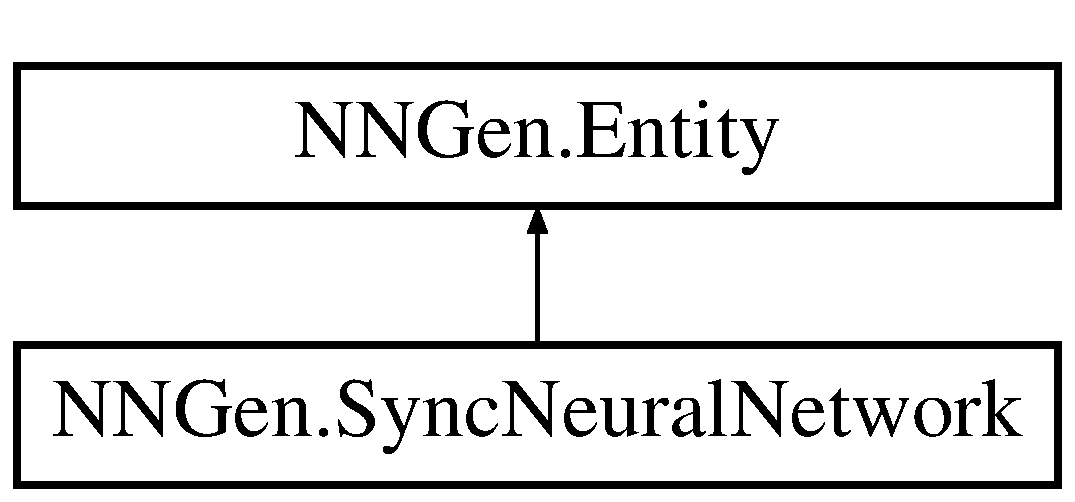
\includegraphics[height=2.000000cm]{class_n_n_gen_1_1_sync_neural_network}
\end{center}
\end{figure}
\subsection*{Public Member Functions}
\begin{DoxyCompactItemize}
\item 
\hyperlink{class_n_n_gen_1_1_sync_neural_network_a668e06ab5c0814666d34e5d5fddce9dc}{Sync\+Neural\+Network} (int\mbox{[}$\,$\mbox{]} \+\_\+neuron\+Counts, double\mbox{[}$\,$\mbox{]} \+\_\+bias\+Values, \hyperlink{class_n_n_gen_1_1_transfer_function_wrapper_aa338ffadb8fcdf76df75419374a51ff6}{Transfer\+Function\+Wrapper.\+Memory\+Activation\+Type}\mbox{[}$\,$\mbox{]} \+\_\+activation\+Types, int \+\_\+num\+Int\+Bits, int \+\_\+num\+Frac\+Bits, int \+\_\+num\+Weight\+Upper\+Bits, bool \+\_\+is\+Classifier, double\mbox{[}$\,$\mbox{]} \+\_\+classifier\+Thresholds, List$<$ double $>$ \+\_\+weights)
\begin{DoxyCompactList}\small\item\em The constructor for a neural network object. Calling this method\textquotesingle{}s write() function will write the entire network. \end{DoxyCompactList}\item 
override string \hyperlink{class_n_n_gen_1_1_sync_neural_network_a91d58e0d612c6398c3164dee0fc34347}{get\+Name} ()
\begin{DoxyCompactList}\small\item\em Returns the name of the entity. \end{DoxyCompactList}\item 
override \hyperlink{class_n_n_gen_1_1_port}{Port}\mbox{[}$\,$\mbox{]} \hyperlink{class_n_n_gen_1_1_sync_neural_network_a8ed253e22e640d3ec0501dd1c43ad784}{get\+Input\+Ports} ()
\begin{DoxyCompactList}\small\item\em Returns the input ports of the entity. \end{DoxyCompactList}\item 
override \hyperlink{class_n_n_gen_1_1_port}{Port}\mbox{[}$\,$\mbox{]} \hyperlink{class_n_n_gen_1_1_sync_neural_network_aff93a78db054336cfe8b2f43885f145d}{get\+Output\+Ports} ()
\begin{DoxyCompactList}\small\item\em Returns the output ports of the entity. \end{DoxyCompactList}\item 
override \hyperlink{class_n_n_gen_1_1_signal}{Signal}\mbox{[}$\,$\mbox{]} \hyperlink{class_n_n_gen_1_1_sync_neural_network_a9303b53dc2d792c18ffa72e386eb0eae}{get\+Internal\+Signals} ()
\begin{DoxyCompactList}\small\item\em Returns the internal signals of the entity. \end{DoxyCompactList}\item 
override bool \hyperlink{class_n_n_gen_1_1_sync_neural_network_ab236b9511b805fa1cabe60f3a2c871d6}{write\+V\+H\+D\+L} (string file)
\begin{DoxyCompactList}\small\item\em Writes the .vhd files necessary to compile this entity. All other necessary entities (i.\+e. neurons, thresholding functions, etc.) will also be written when this function returns \end{DoxyCompactList}\end{DoxyCompactItemize}
\subsection*{Public Attributes}
\begin{DoxyCompactItemize}
\item 
\hyperlink{class_n_n_gen_1_1_sync_neuron}{Sync\+Neuron}\mbox{[}$\,$\mbox{]} \hyperlink{class_n_n_gen_1_1_sync_neural_network_a6358777de50d4b9fafde5b88bc9b96f7}{neurons}
\begin{DoxyCompactList}\small\item\em An array of neurons to implement in the design. The i-\/th element corresponds for the neuron object in the i-\/th row \end{DoxyCompactList}\end{DoxyCompactItemize}
\subsection*{Properties}
\begin{DoxyCompactItemize}
\item 
\hyperlink{class_n_n_gen_1_1_port}{Port}\mbox{[}$\,$\mbox{]} \hyperlink{class_n_n_gen_1_1_sync_neural_network_a6d72194820925ead7f84387e53390f9d}{nn\+Input\+Ports}\hspace{0.3cm}{\ttfamily  \mbox{[}get\mbox{]}}
\begin{DoxyCompactList}\small\item\em The list of input ports to the network \end{DoxyCompactList}\item 
\hyperlink{class_n_n_gen_1_1_port}{Port}\mbox{[}$\,$\mbox{]} \hyperlink{class_n_n_gen_1_1_sync_neural_network_a9e0690fdd6bd2ee365d76b2b9d3ad593}{nn\+Output\+Ports}\hspace{0.3cm}{\ttfamily  \mbox{[}get\mbox{]}}
\begin{DoxyCompactList}\small\item\em The list of output ports to the network \end{DoxyCompactList}\item 
\hyperlink{class_n_n_gen_1_1_port}{Port} \hyperlink{class_n_n_gen_1_1_sync_neural_network_a6306a2d9e689ed32c74ccc5222284315}{ready}\hspace{0.3cm}{\ttfamily  \mbox{[}get\mbox{]}}
\begin{DoxyCompactList}\small\item\em This signal will go high when the network has been initialized after a reset. It will go low when the device is in reset \end{DoxyCompactList}\item 
\hyperlink{class_n_n_gen_1_1_port}{Port} \hyperlink{class_n_n_gen_1_1_sync_neural_network_ab3381bb9b85c8a08ff4f31a123c9c246}{clk}\hspace{0.3cm}{\ttfamily  \mbox{[}get\mbox{]}}
\begin{DoxyCompactList}\small\item\em A clock used for synchronous loading of the neuron weights from memory \end{DoxyCompactList}\item 
\hyperlink{class_n_n_gen_1_1_port}{Port} \hyperlink{class_n_n_gen_1_1_sync_neural_network_a6479fe503fb64dead6508c80c773b042}{reset}\hspace{0.3cm}{\ttfamily  \mbox{[}get\mbox{]}}
\begin{DoxyCompactList}\small\item\em An active high reset for the network \end{DoxyCompactList}\item 
\hyperlink{class_n_n_gen_1_1_transfer_function_wrapper_aa338ffadb8fcdf76df75419374a51ff6}{Transfer\+Function\+Wrapper.\+Memory\+Activation\+Type}\mbox{[}$\,$\mbox{]} \hyperlink{class_n_n_gen_1_1_sync_neural_network_ab9c0e21b58643ab79c5a540181f91a09}{activation\+Types}\hspace{0.3cm}{\ttfamily  \mbox{[}get\mbox{]}}
\begin{DoxyCompactList}\small\item\em The activation types for each layer of the network. The i-\/th member corresponds to the activations of the i-\/th layer of the network \end{DoxyCompactList}\item 
int\mbox{[}$\,$\mbox{]} \hyperlink{class_n_n_gen_1_1_sync_neural_network_aed5af731ce355a68af7607477e8544e9}{neuron\+Counts}\hspace{0.3cm}{\ttfamily  \mbox{[}get\mbox{]}}
\begin{DoxyCompactList}\small\item\em The number of neurons in each layer of the network. The i-\/th member corresponds to the i-\/th layer of the network \end{DoxyCompactList}\item 
double\mbox{[}$\,$\mbox{]} \hyperlink{class_n_n_gen_1_1_sync_neural_network_ae766b78572c54e97ec3be60f7d623dc7}{bias\+Values}\hspace{0.3cm}{\ttfamily  \mbox{[}get\mbox{]}}
\begin{DoxyCompactList}\small\item\em The bias values for each layer. The i-\/th member corresponds to the bias value fed into the i+1-\/th layer of the network \end{DoxyCompactList}\item 
List$<$ \hyperlink{class_n_n_gen_1_1_transfer_function_wrapper}{Transfer\+Function\+Wrapper} $>$ \hyperlink{class_n_n_gen_1_1_sync_neural_network_ad94e116de1c91c9e5f6deb61df5bb23f}{Transfer\+Function\+Wrappers}\hspace{0.3cm}{\ttfamily  \mbox{[}get\mbox{]}}
\begin{DoxyCompactList}\small\item\em The Transfer\+Function\+Wrappers to implement in the final design \end{DoxyCompactList}\item 
Sorted\+Dictionary$<$ int, \hyperlink{class_n_n_gen_1_1_signal}{Signal} $>$ \hyperlink{class_n_n_gen_1_1_sync_neural_network_a76ca03cc953d58f1b392cb723fe3e86a}{Transfer\+Function\+Memories\+Outputs}\hspace{0.3cm}{\ttfamily  \mbox{[}get\mbox{]}}
\begin{DoxyCompactList}\small\item\em A mapping between the output of the neuron layer and the transfer function to use \end{DoxyCompactList}\item 
\hyperlink{class_n_n_gen_1_1_weight_memory}{Weight\+Memory} \hyperlink{class_n_n_gen_1_1_sync_neural_network_a372529d19a342c3636c76319bc91af9a}{weight\+Memory}\hspace{0.3cm}{\ttfamily  \mbox{[}get\mbox{]}}
\begin{DoxyCompactList}\small\item\em A memory instance for the neuron weights \end{DoxyCompactList}\item 
\hyperlink{class_n_n_gen_1_1_signal}{Signal}\mbox{[}$\,$\mbox{]} \hyperlink{class_n_n_gen_1_1_sync_neural_network_ac94c01526c4547dd8bf1e0b18d23dde9}{input\+\_\+latched}\hspace{0.3cm}{\ttfamily  \mbox{[}get\mbox{]}}
\begin{DoxyCompactList}\small\item\em The latches for the inputs to the network. The inputs are sampled once each time the network is run; latching ensures that they remain constant while the network is in operation \end{DoxyCompactList}\item 
\hyperlink{class_n_n_gen_1_1_signal}{Signal}\mbox{[}$\,$\mbox{]} \hyperlink{class_n_n_gen_1_1_sync_neural_network_a9d1fb07536404577262d6c5ccecf2361}{output\+\_\+latched}\hspace{0.3cm}{\ttfamily  \mbox{[}get\mbox{]}}
\begin{DoxyCompactList}\small\item\em The latches for the output to the network. Ensures that the outputs don\textquotesingle{}t fluctuate while the network is computing \end{DoxyCompactList}\item 
\hyperlink{class_n_n_gen_1_1_array_signal}{Array\+Signal} \hyperlink{class_n_n_gen_1_1_sync_neural_network_ad10e93be47aead04db2b445124bb6649}{Neuron\+Outputs}\hspace{0.3cm}{\ttfamily  \mbox{[}get\mbox{]}}
\begin{DoxyCompactList}\small\item\em An array of outputs for each of the neurons \end{DoxyCompactList}\item 
\hyperlink{class_n_n_gen_1_1_array_signal}{Array\+Signal} \hyperlink{class_n_n_gen_1_1_sync_neural_network_a6edeb1a10c731dbc74be6e227201deb0}{Thresh\+Neuron\+Outputs}\hspace{0.3cm}{\ttfamily  \mbox{[}get\mbox{]}}
\begin{DoxyCompactList}\small\item\em The output of the neurons after they\textquotesingle{}ve been run thorugh the respective thresholding functions \end{DoxyCompactList}\item 
\hyperlink{class_n_n_gen_1_1_signal}{Signal} \hyperlink{class_n_n_gen_1_1_sync_neural_network_ac41b8c6d91dd8c38f1bc6800890ed099}{Current\+Neuron\+Output}\hspace{0.3cm}{\ttfamily  \mbox{[}get\mbox{]}}
\begin{DoxyCompactList}\small\item\em The current neuron output to feed into the thresholding function \end{DoxyCompactList}\item 
\hyperlink{class_n_n_gen_1_1_signal}{Signal} \hyperlink{class_n_n_gen_1_1_sync_neural_network_a79c1844f10a33887abfdae4506524e61}{Current\+Thresh\+Neuron\+Output}\hspace{0.3cm}{\ttfamily  \mbox{[}get\mbox{]}}
\begin{DoxyCompactList}\small\item\em The current neuron output from the thresholding function \end{DoxyCompactList}\item 
\hyperlink{class_n_n_gen_1_1_signal}{Signal} \hyperlink{class_n_n_gen_1_1_sync_neural_network_ac2ec6cef24b9127af62c98111bc8ce95}{internal\+Ready}\hspace{0.3cm}{\ttfamily  \mbox{[}get\mbox{]}}
\begin{DoxyCompactList}\small\item\em A signal to determine whether the network has been loaded with the weights and is ready to accept inputs \end{DoxyCompactList}\item 
\hyperlink{class_n_n_gen_1_1_signal}{Signal} \hyperlink{class_n_n_gen_1_1_sync_neural_network_aed787094117713be3ef2eaa612e321e1}{W\+M\+Out}\hspace{0.3cm}{\ttfamily  \mbox{[}get\mbox{]}}
\begin{DoxyCompactList}\small\item\em The output of the weight memory \end{DoxyCompactList}\item 
\hyperlink{class_n_n_gen_1_1_signal}{Signal} \hyperlink{class_n_n_gen_1_1_sync_neural_network_a69b1e243c9d77ba27a38e3859147f588}{Load\+Val}\hspace{0.3cm}{\ttfamily  \mbox{[}get\mbox{]}}
\begin{DoxyCompactList}\small\item\em The value of the output of the weight memory to be loaded into the neuron \end{DoxyCompactList}\item 
\hyperlink{class_n_n_gen_1_1_signal}{Signal} \hyperlink{class_n_n_gen_1_1_sync_neural_network_af587100e0516b187c280dc23b2c226e0}{Load\+Off}\hspace{0.3cm}{\ttfamily  \mbox{[}get\mbox{]}}
\begin{DoxyCompactList}\small\item\em The offset in the neuron\textquotesingle{}s memory at which the memory is to be loaded \end{DoxyCompactList}\item 
\hyperlink{class_n_n_gen_1_1_signal}{Signal} \hyperlink{class_n_n_gen_1_1_sync_neural_network_a26d6d7d846eadc650f466ec37b69c2cb}{W\+M\+Addr}\hspace{0.3cm}{\ttfamily  \mbox{[}get\mbox{]}}
\begin{DoxyCompactList}\small\item\em The address from which to read in the weight memory \end{DoxyCompactList}\item 
\hyperlink{class_n_n_gen_1_1_signal}{Signal} \hyperlink{class_n_n_gen_1_1_sync_neural_network_adde5cc8cf981b7e6dd24ddcb0193cd9a}{Hold\+W\+M}\hspace{0.3cm}{\ttfamily  \mbox{[}get\mbox{]}}
\begin{DoxyCompactList}\small\item\em When high, pauses the W\+M clk signal. Needed during the load process to avoid skipping weights \end{DoxyCompactList}\item 
\hyperlink{class_n_n_gen_1_1_signal}{Signal} \hyperlink{class_n_n_gen_1_1_sync_neural_network_ad0473c03570ed0231da8b2d62487b99a}{W\+M\+Clk}\hspace{0.3cm}{\ttfamily  \mbox{[}get\mbox{]}}
\begin{DoxyCompactList}\small\item\em The clock signal for the weight memory. \end{DoxyCompactList}\item 
\hyperlink{class_n_n_gen_1_1_signal}{Signal} \hyperlink{class_n_n_gen_1_1_sync_neural_network_a3d9360657f0a709cc8682eac7465e96f}{Activate\+Sig}\hspace{0.3cm}{\ttfamily  \mbox{[}get\mbox{]}}
\begin{DoxyCompactList}\small\item\em A signal used to determine which neurons are active. When the i-\/th bit is \textquotesingle{}1\textquotesingle{}, the i-\/th layer is computing \end{DoxyCompactList}\item 
\hyperlink{class_n_n_gen_1_1_signal}{Signal} \hyperlink{class_n_n_gen_1_1_sync_neural_network_a6671f2beb14d4e2f2cec90c79046f656}{Clock\+Count}\hspace{0.3cm}{\ttfamily  \mbox{[}get\mbox{]}}
\begin{DoxyCompactList}\small\item\em A counter used to compute when the different bits of Activate\+Sig should be set \end{DoxyCompactList}\item 
\hyperlink{class_n_n_gen_1_1_signal}{Signal} \hyperlink{class_n_n_gen_1_1_sync_neural_network_a0da1ffac1794b37b1b27b81fd03253a3}{Final\+Loads}\hspace{0.3cm}{\ttfamily  \mbox{[}get\mbox{]}}
\begin{DoxyCompactList}\small\item\em A signal to hold the Final\+Load signals from the neurons \end{DoxyCompactList}\item 
\hyperlink{class_n_n_gen_1_1_signal}{Signal} \hyperlink{class_n_n_gen_1_1_sync_neural_network_a5005f0c6c9b6377dfc66c2894251f4dd}{Load\+Enables}\hspace{0.3cm}{\ttfamily  \mbox{[}get\mbox{]}}
\begin{DoxyCompactList}\small\item\em A signal used to enable or disable loading of the weights of a neuron \end{DoxyCompactList}\item 
List$<$ \hyperlink{class_n_n_gen_1_1_signal}{Signal} $>$ \hyperlink{class_n_n_gen_1_1_sync_neural_network_a5d11d979c5498deaa585533ef25883ce}{transfer\+Fxn\+Outputs}\hspace{0.3cm}{\ttfamily  \mbox{[}get\mbox{]}}
\begin{DoxyCompactList}\small\item\em The outputs from the Transfer\+Function\+Memory\+Wrappers. Eventually multiplexed into Current\+Thresh\+Neuron\+Output \end{DoxyCompactList}\item 
bool \hyperlink{class_n_n_gen_1_1_sync_neural_network_ac4b6c7f973b66d41e7e12795b027887d}{is\+Classifier}\hspace{0.3cm}{\ttfamily  \mbox{[}get\mbox{]}}
\begin{DoxyCompactList}\small\item\em If the neural network is to be used for classification, then this variable should be set to true. This will instantiate comparitors on the output neurons. \end{DoxyCompactList}\item 
int \hyperlink{class_n_n_gen_1_1_sync_neural_network_a66e287c50de3ae1932ea768fc3fa54fc}{num\+Int\+Bits}\hspace{0.3cm}{\ttfamily  \mbox{[}get\mbox{]}}
\begin{DoxyCompactList}\small\item\em The number of integer bits to be used for the neural network inputs \end{DoxyCompactList}\item 
int \hyperlink{class_n_n_gen_1_1_sync_neural_network_a82e208d521ab24cb49b0fdfa1ed285c1}{num\+Frac\+Bits}\hspace{0.3cm}{\ttfamily  \mbox{[}get\mbox{]}}
\begin{DoxyCompactList}\small\item\em The number of fractional bits to be used for the neural network inputs and for the neural network weights \end{DoxyCompactList}\item 
int \hyperlink{class_n_n_gen_1_1_sync_neural_network_afe97a4c00e87742409fe9a5a16922822}{num\+Weight\+Upper\+Bits}\hspace{0.3cm}{\ttfamily  \mbox{[}get\mbox{]}}
\begin{DoxyCompactList}\small\item\em The number of integer bits to be used for the neural network weights. \end{DoxyCompactList}\item 
double\mbox{[}$\,$\mbox{]} \hyperlink{class_n_n_gen_1_1_sync_neural_network_ad044d0ce18e20de41ea9c30ad30b96b1}{classifier\+Thresholds}\hspace{0.3cm}{\ttfamily  \mbox{[}get\mbox{]}}
\begin{DoxyCompactList}\small\item\em The values to be used for thresholding the output neurons. The i-\/th member of this array corresponds to the theshold value for the i-\/th output neuron. If the network is not a classification network (i.\+e. is\+Classifier = false), then this member is unused. \end{DoxyCompactList}\end{DoxyCompactItemize}


\subsection{Detailed Description}
A class representing a synchronous neural network 



\subsection{Constructor \& Destructor Documentation}
\hypertarget{class_n_n_gen_1_1_sync_neural_network_a668e06ab5c0814666d34e5d5fddce9dc}{}\index{N\+N\+Gen\+::\+Sync\+Neural\+Network@{N\+N\+Gen\+::\+Sync\+Neural\+Network}!Sync\+Neural\+Network@{Sync\+Neural\+Network}}
\index{Sync\+Neural\+Network@{Sync\+Neural\+Network}!N\+N\+Gen\+::\+Sync\+Neural\+Network@{N\+N\+Gen\+::\+Sync\+Neural\+Network}}
\subsubsection[{Sync\+Neural\+Network(int[] \+\_\+neuron\+Counts, double[] \+\_\+bias\+Values, Transfer\+Function\+Wrapper.\+Memory\+Activation\+Type[] \+\_\+activation\+Types, int \+\_\+num\+Int\+Bits, int \+\_\+num\+Frac\+Bits, int \+\_\+num\+Weight\+Upper\+Bits, bool \+\_\+is\+Classifier, double[] \+\_\+classifier\+Thresholds, List$<$ double $>$ \+\_\+weights)}]{\setlength{\rightskip}{0pt plus 5cm}N\+N\+Gen.\+Sync\+Neural\+Network.\+Sync\+Neural\+Network (
\begin{DoxyParamCaption}
\item[{int\mbox{[}$\,$\mbox{]}}]{\+\_\+neuron\+Counts, }
\item[{double\mbox{[}$\,$\mbox{]}}]{\+\_\+bias\+Values, }
\item[{{\bf Transfer\+Function\+Wrapper.\+Memory\+Activation\+Type}\mbox{[}$\,$\mbox{]}}]{\+\_\+activation\+Types, }
\item[{int}]{\+\_\+num\+Int\+Bits, }
\item[{int}]{\+\_\+num\+Frac\+Bits, }
\item[{int}]{\+\_\+num\+Weight\+Upper\+Bits, }
\item[{bool}]{\+\_\+is\+Classifier, }
\item[{double\mbox{[}$\,$\mbox{]}}]{\+\_\+classifier\+Thresholds, }
\item[{List$<$ double $>$}]{\+\_\+weights}
\end{DoxyParamCaption}
)\hspace{0.3cm}{\ttfamily [inline]}}\label{class_n_n_gen_1_1_sync_neural_network_a668e06ab5c0814666d34e5d5fddce9dc}


The constructor for a neural network object. Calling this method\textquotesingle{}s write() function will write the entire network. 


\begin{DoxyParams}{Parameters}
{\em \+\_\+neuron\+Counts} & The number of neurons in each layer, excluding the bias node.\\
\hline
{\em \+\_\+bias\+Values} & The bias value feeding forward into the next layer. \\
\hline
{\em \+\_\+activation\+Types} & The activation types for the neurons in each layer\\
\hline
{\em \+\_\+num\+Int\+Bits} & The number of integer bits to use for the inputs for each neuron (Sigmoid activated neurons automatically get this set to zero)\\
\hline
{\em \+\_\+num\+Frac\+Bits} & The number of fractional bits to use for the inputs for each neuron\\
\hline
{\em \+\_\+num\+Weight\+Upper\+Bits} & The number of integer bits used for the weights for each neuron.\\
\hline
{\em \+\_\+is\+Classifier} & If true, a comparitor will be instantiatated at the output to each node, comparing the output layer nodes to the threshold value.\\
\hline
{\em \+\_\+classifier\+Thresholds} & The threshold values for the output comparitors\\
\hline
{\em \+\_\+weights} & The list of weights read in for the neurons from Weight\+Reader.\+read\+Weights\+From\+File()\\
\hline
\end{DoxyParams}
$<$remark$>$ For example, to intialize a classification neural network with three inputs, two hidden sigmoid-\/activated nodes, and one linear output node, use the following line\+:$<$/remark$>$ 

Neural\+Network nn = new Neural\+Network(\mbox{[}3, 2, 1\mbox{]}, \mbox{[}-\/1, -\/1\mbox{]}, \mbox{[}..S\+I\+G\+M\+O\+I\+D\+\_\+\+P\+O\+L\+Y\+\_\+\+A\+P\+P\+R\+O\+X, ..L\+I\+N\+E\+A\+R\mbox{]}, 4, 4, 4, true, \mbox{[}0.\+5\mbox{]}, \+\_\+weights);

\subsection{Member Function Documentation}
\hypertarget{class_n_n_gen_1_1_sync_neural_network_a8ed253e22e640d3ec0501dd1c43ad784}{}\index{N\+N\+Gen\+::\+Sync\+Neural\+Network@{N\+N\+Gen\+::\+Sync\+Neural\+Network}!get\+Input\+Ports@{get\+Input\+Ports}}
\index{get\+Input\+Ports@{get\+Input\+Ports}!N\+N\+Gen\+::\+Sync\+Neural\+Network@{N\+N\+Gen\+::\+Sync\+Neural\+Network}}
\subsubsection[{get\+Input\+Ports()}]{\setlength{\rightskip}{0pt plus 5cm}override {\bf Port} \mbox{[}$\,$\mbox{]} N\+N\+Gen.\+Sync\+Neural\+Network.\+get\+Input\+Ports (
\begin{DoxyParamCaption}
{}
\end{DoxyParamCaption}
)\hspace{0.3cm}{\ttfamily [inline]}, {\ttfamily [virtual]}}\label{class_n_n_gen_1_1_sync_neural_network_a8ed253e22e640d3ec0501dd1c43ad784}


Returns the input ports of the entity. 

\begin{DoxyReturn}{Returns}
The input ports of the entity
\end{DoxyReturn}


Implements \hyperlink{class_n_n_gen_1_1_entity_a01239f05c9efa61ec9e6a29cb2eaad50}{N\+N\+Gen.\+Entity}.

\hypertarget{class_n_n_gen_1_1_sync_neural_network_a9303b53dc2d792c18ffa72e386eb0eae}{}\index{N\+N\+Gen\+::\+Sync\+Neural\+Network@{N\+N\+Gen\+::\+Sync\+Neural\+Network}!get\+Internal\+Signals@{get\+Internal\+Signals}}
\index{get\+Internal\+Signals@{get\+Internal\+Signals}!N\+N\+Gen\+::\+Sync\+Neural\+Network@{N\+N\+Gen\+::\+Sync\+Neural\+Network}}
\subsubsection[{get\+Internal\+Signals()}]{\setlength{\rightskip}{0pt plus 5cm}override {\bf Signal} \mbox{[}$\,$\mbox{]} N\+N\+Gen.\+Sync\+Neural\+Network.\+get\+Internal\+Signals (
\begin{DoxyParamCaption}
{}
\end{DoxyParamCaption}
)\hspace{0.3cm}{\ttfamily [inline]}, {\ttfamily [virtual]}}\label{class_n_n_gen_1_1_sync_neural_network_a9303b53dc2d792c18ffa72e386eb0eae}


Returns the internal signals of the entity. 

\begin{DoxyReturn}{Returns}
The internal signals of the entity
\end{DoxyReturn}


Implements \hyperlink{class_n_n_gen_1_1_entity_a62feb80e95ec84c650ea17bd53f0d510}{N\+N\+Gen.\+Entity}.

\hypertarget{class_n_n_gen_1_1_sync_neural_network_a91d58e0d612c6398c3164dee0fc34347}{}\index{N\+N\+Gen\+::\+Sync\+Neural\+Network@{N\+N\+Gen\+::\+Sync\+Neural\+Network}!get\+Name@{get\+Name}}
\index{get\+Name@{get\+Name}!N\+N\+Gen\+::\+Sync\+Neural\+Network@{N\+N\+Gen\+::\+Sync\+Neural\+Network}}
\subsubsection[{get\+Name()}]{\setlength{\rightskip}{0pt plus 5cm}override string N\+N\+Gen.\+Sync\+Neural\+Network.\+get\+Name (
\begin{DoxyParamCaption}
{}
\end{DoxyParamCaption}
)\hspace{0.3cm}{\ttfamily [inline]}, {\ttfamily [virtual]}}\label{class_n_n_gen_1_1_sync_neural_network_a91d58e0d612c6398c3164dee0fc34347}


Returns the name of the entity. 

\begin{DoxyReturn}{Returns}
The name of the entity
\end{DoxyReturn}


Implements \hyperlink{class_n_n_gen_1_1_entity_a9f25d1070c9ab8ad343c28443e62e6f2}{N\+N\+Gen.\+Entity}.

\hypertarget{class_n_n_gen_1_1_sync_neural_network_aff93a78db054336cfe8b2f43885f145d}{}\index{N\+N\+Gen\+::\+Sync\+Neural\+Network@{N\+N\+Gen\+::\+Sync\+Neural\+Network}!get\+Output\+Ports@{get\+Output\+Ports}}
\index{get\+Output\+Ports@{get\+Output\+Ports}!N\+N\+Gen\+::\+Sync\+Neural\+Network@{N\+N\+Gen\+::\+Sync\+Neural\+Network}}
\subsubsection[{get\+Output\+Ports()}]{\setlength{\rightskip}{0pt plus 5cm}override {\bf Port} \mbox{[}$\,$\mbox{]} N\+N\+Gen.\+Sync\+Neural\+Network.\+get\+Output\+Ports (
\begin{DoxyParamCaption}
{}
\end{DoxyParamCaption}
)\hspace{0.3cm}{\ttfamily [inline]}, {\ttfamily [virtual]}}\label{class_n_n_gen_1_1_sync_neural_network_aff93a78db054336cfe8b2f43885f145d}


Returns the output ports of the entity. 

\begin{DoxyReturn}{Returns}
The output ports of the entity
\end{DoxyReturn}


Implements \hyperlink{class_n_n_gen_1_1_entity_ace06368087778e254a5048c7d28747be}{N\+N\+Gen.\+Entity}.

\hypertarget{class_n_n_gen_1_1_sync_neural_network_ab236b9511b805fa1cabe60f3a2c871d6}{}\index{N\+N\+Gen\+::\+Sync\+Neural\+Network@{N\+N\+Gen\+::\+Sync\+Neural\+Network}!write\+V\+H\+D\+L@{write\+V\+H\+D\+L}}
\index{write\+V\+H\+D\+L@{write\+V\+H\+D\+L}!N\+N\+Gen\+::\+Sync\+Neural\+Network@{N\+N\+Gen\+::\+Sync\+Neural\+Network}}
\subsubsection[{write\+V\+H\+D\+L(string file)}]{\setlength{\rightskip}{0pt plus 5cm}override bool N\+N\+Gen.\+Sync\+Neural\+Network.\+write\+V\+H\+D\+L (
\begin{DoxyParamCaption}
\item[{string}]{file}
\end{DoxyParamCaption}
)\hspace{0.3cm}{\ttfamily [inline]}, {\ttfamily [virtual]}}\label{class_n_n_gen_1_1_sync_neural_network_ab236b9511b805fa1cabe60f3a2c871d6}


Writes the .vhd files necessary to compile this entity. All other necessary entities (i.\+e. neurons, thresholding functions, etc.) will also be written when this function returns 


\begin{DoxyParams}{Parameters}
{\em file} & The file path in which to write the files (do N\+O\+T include \char`\"{}...\+name.\+vhd\char`\"{}\\
\hline
\end{DoxyParams}
\begin{DoxyReturn}{Returns}
true if the files were written successfully, false otherwise
\end{DoxyReturn}


Implements \hyperlink{class_n_n_gen_1_1_entity_a1111d498446be08b20583b9625893a52}{N\+N\+Gen.\+Entity}.



\subsection{Member Data Documentation}
\hypertarget{class_n_n_gen_1_1_sync_neural_network_a6358777de50d4b9fafde5b88bc9b96f7}{}\index{N\+N\+Gen\+::\+Sync\+Neural\+Network@{N\+N\+Gen\+::\+Sync\+Neural\+Network}!neurons@{neurons}}
\index{neurons@{neurons}!N\+N\+Gen\+::\+Sync\+Neural\+Network@{N\+N\+Gen\+::\+Sync\+Neural\+Network}}
\subsubsection[{neurons}]{\setlength{\rightskip}{0pt plus 5cm}{\bf Sync\+Neuron} \mbox{[}$\,$\mbox{]} N\+N\+Gen.\+Sync\+Neural\+Network.\+neurons}\label{class_n_n_gen_1_1_sync_neural_network_a6358777de50d4b9fafde5b88bc9b96f7}


An array of neurons to implement in the design. The i-\/th element corresponds for the neuron object in the i-\/th row 



\subsection{Property Documentation}
\hypertarget{class_n_n_gen_1_1_sync_neural_network_a3d9360657f0a709cc8682eac7465e96f}{}\index{N\+N\+Gen\+::\+Sync\+Neural\+Network@{N\+N\+Gen\+::\+Sync\+Neural\+Network}!Activate\+Sig@{Activate\+Sig}}
\index{Activate\+Sig@{Activate\+Sig}!N\+N\+Gen\+::\+Sync\+Neural\+Network@{N\+N\+Gen\+::\+Sync\+Neural\+Network}}
\subsubsection[{Activate\+Sig}]{\setlength{\rightskip}{0pt plus 5cm}{\bf Signal} N\+N\+Gen.\+Sync\+Neural\+Network.\+Activate\+Sig\hspace{0.3cm}{\ttfamily [get]}}\label{class_n_n_gen_1_1_sync_neural_network_a3d9360657f0a709cc8682eac7465e96f}


A signal used to determine which neurons are active. When the i-\/th bit is \textquotesingle{}1\textquotesingle{}, the i-\/th layer is computing 

\hypertarget{class_n_n_gen_1_1_sync_neural_network_ab9c0e21b58643ab79c5a540181f91a09}{}\index{N\+N\+Gen\+::\+Sync\+Neural\+Network@{N\+N\+Gen\+::\+Sync\+Neural\+Network}!activation\+Types@{activation\+Types}}
\index{activation\+Types@{activation\+Types}!N\+N\+Gen\+::\+Sync\+Neural\+Network@{N\+N\+Gen\+::\+Sync\+Neural\+Network}}
\subsubsection[{activation\+Types}]{\setlength{\rightskip}{0pt plus 5cm}{\bf Transfer\+Function\+Wrapper.\+Memory\+Activation\+Type} \mbox{[}$\,$\mbox{]} N\+N\+Gen.\+Sync\+Neural\+Network.\+activation\+Types\hspace{0.3cm}{\ttfamily [get]}}\label{class_n_n_gen_1_1_sync_neural_network_ab9c0e21b58643ab79c5a540181f91a09}


The activation types for each layer of the network. The i-\/th member corresponds to the activations of the i-\/th layer of the network 

\hypertarget{class_n_n_gen_1_1_sync_neural_network_ae766b78572c54e97ec3be60f7d623dc7}{}\index{N\+N\+Gen\+::\+Sync\+Neural\+Network@{N\+N\+Gen\+::\+Sync\+Neural\+Network}!bias\+Values@{bias\+Values}}
\index{bias\+Values@{bias\+Values}!N\+N\+Gen\+::\+Sync\+Neural\+Network@{N\+N\+Gen\+::\+Sync\+Neural\+Network}}
\subsubsection[{bias\+Values}]{\setlength{\rightskip}{0pt plus 5cm}double \mbox{[}$\,$\mbox{]} N\+N\+Gen.\+Sync\+Neural\+Network.\+bias\+Values\hspace{0.3cm}{\ttfamily [get]}}\label{class_n_n_gen_1_1_sync_neural_network_ae766b78572c54e97ec3be60f7d623dc7}


The bias values for each layer. The i-\/th member corresponds to the bias value fed into the i+1-\/th layer of the network 

\hypertarget{class_n_n_gen_1_1_sync_neural_network_ad044d0ce18e20de41ea9c30ad30b96b1}{}\index{N\+N\+Gen\+::\+Sync\+Neural\+Network@{N\+N\+Gen\+::\+Sync\+Neural\+Network}!classifier\+Thresholds@{classifier\+Thresholds}}
\index{classifier\+Thresholds@{classifier\+Thresholds}!N\+N\+Gen\+::\+Sync\+Neural\+Network@{N\+N\+Gen\+::\+Sync\+Neural\+Network}}
\subsubsection[{classifier\+Thresholds}]{\setlength{\rightskip}{0pt plus 5cm}double \mbox{[}$\,$\mbox{]} N\+N\+Gen.\+Sync\+Neural\+Network.\+classifier\+Thresholds\hspace{0.3cm}{\ttfamily [get]}}\label{class_n_n_gen_1_1_sync_neural_network_ad044d0ce18e20de41ea9c30ad30b96b1}


The values to be used for thresholding the output neurons. The i-\/th member of this array corresponds to the theshold value for the i-\/th output neuron. If the network is not a classification network (i.\+e. is\+Classifier = false), then this member is unused. 

\hypertarget{class_n_n_gen_1_1_sync_neural_network_ab3381bb9b85c8a08ff4f31a123c9c246}{}\index{N\+N\+Gen\+::\+Sync\+Neural\+Network@{N\+N\+Gen\+::\+Sync\+Neural\+Network}!clk@{clk}}
\index{clk@{clk}!N\+N\+Gen\+::\+Sync\+Neural\+Network@{N\+N\+Gen\+::\+Sync\+Neural\+Network}}
\subsubsection[{clk}]{\setlength{\rightskip}{0pt plus 5cm}{\bf Port} N\+N\+Gen.\+Sync\+Neural\+Network.\+clk\hspace{0.3cm}{\ttfamily [get]}}\label{class_n_n_gen_1_1_sync_neural_network_ab3381bb9b85c8a08ff4f31a123c9c246}


A clock used for synchronous loading of the neuron weights from memory 

\hypertarget{class_n_n_gen_1_1_sync_neural_network_a6671f2beb14d4e2f2cec90c79046f656}{}\index{N\+N\+Gen\+::\+Sync\+Neural\+Network@{N\+N\+Gen\+::\+Sync\+Neural\+Network}!Clock\+Count@{Clock\+Count}}
\index{Clock\+Count@{Clock\+Count}!N\+N\+Gen\+::\+Sync\+Neural\+Network@{N\+N\+Gen\+::\+Sync\+Neural\+Network}}
\subsubsection[{Clock\+Count}]{\setlength{\rightskip}{0pt plus 5cm}{\bf Signal} N\+N\+Gen.\+Sync\+Neural\+Network.\+Clock\+Count\hspace{0.3cm}{\ttfamily [get]}}\label{class_n_n_gen_1_1_sync_neural_network_a6671f2beb14d4e2f2cec90c79046f656}


A counter used to compute when the different bits of Activate\+Sig should be set 

\hypertarget{class_n_n_gen_1_1_sync_neural_network_ac41b8c6d91dd8c38f1bc6800890ed099}{}\index{N\+N\+Gen\+::\+Sync\+Neural\+Network@{N\+N\+Gen\+::\+Sync\+Neural\+Network}!Current\+Neuron\+Output@{Current\+Neuron\+Output}}
\index{Current\+Neuron\+Output@{Current\+Neuron\+Output}!N\+N\+Gen\+::\+Sync\+Neural\+Network@{N\+N\+Gen\+::\+Sync\+Neural\+Network}}
\subsubsection[{Current\+Neuron\+Output}]{\setlength{\rightskip}{0pt plus 5cm}{\bf Signal} N\+N\+Gen.\+Sync\+Neural\+Network.\+Current\+Neuron\+Output\hspace{0.3cm}{\ttfamily [get]}}\label{class_n_n_gen_1_1_sync_neural_network_ac41b8c6d91dd8c38f1bc6800890ed099}


The current neuron output to feed into the thresholding function 

\hypertarget{class_n_n_gen_1_1_sync_neural_network_a79c1844f10a33887abfdae4506524e61}{}\index{N\+N\+Gen\+::\+Sync\+Neural\+Network@{N\+N\+Gen\+::\+Sync\+Neural\+Network}!Current\+Thresh\+Neuron\+Output@{Current\+Thresh\+Neuron\+Output}}
\index{Current\+Thresh\+Neuron\+Output@{Current\+Thresh\+Neuron\+Output}!N\+N\+Gen\+::\+Sync\+Neural\+Network@{N\+N\+Gen\+::\+Sync\+Neural\+Network}}
\subsubsection[{Current\+Thresh\+Neuron\+Output}]{\setlength{\rightskip}{0pt plus 5cm}{\bf Signal} N\+N\+Gen.\+Sync\+Neural\+Network.\+Current\+Thresh\+Neuron\+Output\hspace{0.3cm}{\ttfamily [get]}}\label{class_n_n_gen_1_1_sync_neural_network_a79c1844f10a33887abfdae4506524e61}


The current neuron output from the thresholding function 

\hypertarget{class_n_n_gen_1_1_sync_neural_network_a0da1ffac1794b37b1b27b81fd03253a3}{}\index{N\+N\+Gen\+::\+Sync\+Neural\+Network@{N\+N\+Gen\+::\+Sync\+Neural\+Network}!Final\+Loads@{Final\+Loads}}
\index{Final\+Loads@{Final\+Loads}!N\+N\+Gen\+::\+Sync\+Neural\+Network@{N\+N\+Gen\+::\+Sync\+Neural\+Network}}
\subsubsection[{Final\+Loads}]{\setlength{\rightskip}{0pt plus 5cm}{\bf Signal} N\+N\+Gen.\+Sync\+Neural\+Network.\+Final\+Loads\hspace{0.3cm}{\ttfamily [get]}}\label{class_n_n_gen_1_1_sync_neural_network_a0da1ffac1794b37b1b27b81fd03253a3}


A signal to hold the Final\+Load signals from the neurons 

\hypertarget{class_n_n_gen_1_1_sync_neural_network_adde5cc8cf981b7e6dd24ddcb0193cd9a}{}\index{N\+N\+Gen\+::\+Sync\+Neural\+Network@{N\+N\+Gen\+::\+Sync\+Neural\+Network}!Hold\+W\+M@{Hold\+W\+M}}
\index{Hold\+W\+M@{Hold\+W\+M}!N\+N\+Gen\+::\+Sync\+Neural\+Network@{N\+N\+Gen\+::\+Sync\+Neural\+Network}}
\subsubsection[{Hold\+W\+M}]{\setlength{\rightskip}{0pt plus 5cm}{\bf Signal} N\+N\+Gen.\+Sync\+Neural\+Network.\+Hold\+W\+M\hspace{0.3cm}{\ttfamily [get]}}\label{class_n_n_gen_1_1_sync_neural_network_adde5cc8cf981b7e6dd24ddcb0193cd9a}


When high, pauses the W\+M clk signal. Needed during the load process to avoid skipping weights 

\hypertarget{class_n_n_gen_1_1_sync_neural_network_ac94c01526c4547dd8bf1e0b18d23dde9}{}\index{N\+N\+Gen\+::\+Sync\+Neural\+Network@{N\+N\+Gen\+::\+Sync\+Neural\+Network}!input\+\_\+latched@{input\+\_\+latched}}
\index{input\+\_\+latched@{input\+\_\+latched}!N\+N\+Gen\+::\+Sync\+Neural\+Network@{N\+N\+Gen\+::\+Sync\+Neural\+Network}}
\subsubsection[{input\+\_\+latched}]{\setlength{\rightskip}{0pt plus 5cm}{\bf Signal} \mbox{[}$\,$\mbox{]} N\+N\+Gen.\+Sync\+Neural\+Network.\+input\+\_\+latched\hspace{0.3cm}{\ttfamily [get]}}\label{class_n_n_gen_1_1_sync_neural_network_ac94c01526c4547dd8bf1e0b18d23dde9}


The latches for the inputs to the network. The inputs are sampled once each time the network is run; latching ensures that they remain constant while the network is in operation 

\hypertarget{class_n_n_gen_1_1_sync_neural_network_ac2ec6cef24b9127af62c98111bc8ce95}{}\index{N\+N\+Gen\+::\+Sync\+Neural\+Network@{N\+N\+Gen\+::\+Sync\+Neural\+Network}!internal\+Ready@{internal\+Ready}}
\index{internal\+Ready@{internal\+Ready}!N\+N\+Gen\+::\+Sync\+Neural\+Network@{N\+N\+Gen\+::\+Sync\+Neural\+Network}}
\subsubsection[{internal\+Ready}]{\setlength{\rightskip}{0pt plus 5cm}{\bf Signal} N\+N\+Gen.\+Sync\+Neural\+Network.\+internal\+Ready\hspace{0.3cm}{\ttfamily [get]}}\label{class_n_n_gen_1_1_sync_neural_network_ac2ec6cef24b9127af62c98111bc8ce95}


A signal to determine whether the network has been loaded with the weights and is ready to accept inputs 

\hypertarget{class_n_n_gen_1_1_sync_neural_network_ac4b6c7f973b66d41e7e12795b027887d}{}\index{N\+N\+Gen\+::\+Sync\+Neural\+Network@{N\+N\+Gen\+::\+Sync\+Neural\+Network}!is\+Classifier@{is\+Classifier}}
\index{is\+Classifier@{is\+Classifier}!N\+N\+Gen\+::\+Sync\+Neural\+Network@{N\+N\+Gen\+::\+Sync\+Neural\+Network}}
\subsubsection[{is\+Classifier}]{\setlength{\rightskip}{0pt plus 5cm}bool N\+N\+Gen.\+Sync\+Neural\+Network.\+is\+Classifier\hspace{0.3cm}{\ttfamily [get]}}\label{class_n_n_gen_1_1_sync_neural_network_ac4b6c7f973b66d41e7e12795b027887d}


If the neural network is to be used for classification, then this variable should be set to true. This will instantiate comparitors on the output neurons. 

\hypertarget{class_n_n_gen_1_1_sync_neural_network_a5005f0c6c9b6377dfc66c2894251f4dd}{}\index{N\+N\+Gen\+::\+Sync\+Neural\+Network@{N\+N\+Gen\+::\+Sync\+Neural\+Network}!Load\+Enables@{Load\+Enables}}
\index{Load\+Enables@{Load\+Enables}!N\+N\+Gen\+::\+Sync\+Neural\+Network@{N\+N\+Gen\+::\+Sync\+Neural\+Network}}
\subsubsection[{Load\+Enables}]{\setlength{\rightskip}{0pt plus 5cm}{\bf Signal} N\+N\+Gen.\+Sync\+Neural\+Network.\+Load\+Enables\hspace{0.3cm}{\ttfamily [get]}}\label{class_n_n_gen_1_1_sync_neural_network_a5005f0c6c9b6377dfc66c2894251f4dd}


A signal used to enable or disable loading of the weights of a neuron 

\hypertarget{class_n_n_gen_1_1_sync_neural_network_af587100e0516b187c280dc23b2c226e0}{}\index{N\+N\+Gen\+::\+Sync\+Neural\+Network@{N\+N\+Gen\+::\+Sync\+Neural\+Network}!Load\+Off@{Load\+Off}}
\index{Load\+Off@{Load\+Off}!N\+N\+Gen\+::\+Sync\+Neural\+Network@{N\+N\+Gen\+::\+Sync\+Neural\+Network}}
\subsubsection[{Load\+Off}]{\setlength{\rightskip}{0pt plus 5cm}{\bf Signal} N\+N\+Gen.\+Sync\+Neural\+Network.\+Load\+Off\hspace{0.3cm}{\ttfamily [get]}}\label{class_n_n_gen_1_1_sync_neural_network_af587100e0516b187c280dc23b2c226e0}


The offset in the neuron\textquotesingle{}s memory at which the memory is to be loaded 

\hypertarget{class_n_n_gen_1_1_sync_neural_network_a69b1e243c9d77ba27a38e3859147f588}{}\index{N\+N\+Gen\+::\+Sync\+Neural\+Network@{N\+N\+Gen\+::\+Sync\+Neural\+Network}!Load\+Val@{Load\+Val}}
\index{Load\+Val@{Load\+Val}!N\+N\+Gen\+::\+Sync\+Neural\+Network@{N\+N\+Gen\+::\+Sync\+Neural\+Network}}
\subsubsection[{Load\+Val}]{\setlength{\rightskip}{0pt plus 5cm}{\bf Signal} N\+N\+Gen.\+Sync\+Neural\+Network.\+Load\+Val\hspace{0.3cm}{\ttfamily [get]}}\label{class_n_n_gen_1_1_sync_neural_network_a69b1e243c9d77ba27a38e3859147f588}


The value of the output of the weight memory to be loaded into the neuron 

\hypertarget{class_n_n_gen_1_1_sync_neural_network_aed5af731ce355a68af7607477e8544e9}{}\index{N\+N\+Gen\+::\+Sync\+Neural\+Network@{N\+N\+Gen\+::\+Sync\+Neural\+Network}!neuron\+Counts@{neuron\+Counts}}
\index{neuron\+Counts@{neuron\+Counts}!N\+N\+Gen\+::\+Sync\+Neural\+Network@{N\+N\+Gen\+::\+Sync\+Neural\+Network}}
\subsubsection[{neuron\+Counts}]{\setlength{\rightskip}{0pt plus 5cm}int \mbox{[}$\,$\mbox{]} N\+N\+Gen.\+Sync\+Neural\+Network.\+neuron\+Counts\hspace{0.3cm}{\ttfamily [get]}}\label{class_n_n_gen_1_1_sync_neural_network_aed5af731ce355a68af7607477e8544e9}


The number of neurons in each layer of the network. The i-\/th member corresponds to the i-\/th layer of the network 

\hypertarget{class_n_n_gen_1_1_sync_neural_network_ad10e93be47aead04db2b445124bb6649}{}\index{N\+N\+Gen\+::\+Sync\+Neural\+Network@{N\+N\+Gen\+::\+Sync\+Neural\+Network}!Neuron\+Outputs@{Neuron\+Outputs}}
\index{Neuron\+Outputs@{Neuron\+Outputs}!N\+N\+Gen\+::\+Sync\+Neural\+Network@{N\+N\+Gen\+::\+Sync\+Neural\+Network}}
\subsubsection[{Neuron\+Outputs}]{\setlength{\rightskip}{0pt plus 5cm}{\bf Array\+Signal} N\+N\+Gen.\+Sync\+Neural\+Network.\+Neuron\+Outputs\hspace{0.3cm}{\ttfamily [get]}}\label{class_n_n_gen_1_1_sync_neural_network_ad10e93be47aead04db2b445124bb6649}


An array of outputs for each of the neurons 

\hypertarget{class_n_n_gen_1_1_sync_neural_network_a6d72194820925ead7f84387e53390f9d}{}\index{N\+N\+Gen\+::\+Sync\+Neural\+Network@{N\+N\+Gen\+::\+Sync\+Neural\+Network}!nn\+Input\+Ports@{nn\+Input\+Ports}}
\index{nn\+Input\+Ports@{nn\+Input\+Ports}!N\+N\+Gen\+::\+Sync\+Neural\+Network@{N\+N\+Gen\+::\+Sync\+Neural\+Network}}
\subsubsection[{nn\+Input\+Ports}]{\setlength{\rightskip}{0pt plus 5cm}{\bf Port} \mbox{[}$\,$\mbox{]} N\+N\+Gen.\+Sync\+Neural\+Network.\+nn\+Input\+Ports\hspace{0.3cm}{\ttfamily [get]}}\label{class_n_n_gen_1_1_sync_neural_network_a6d72194820925ead7f84387e53390f9d}


The list of input ports to the network 

\hypertarget{class_n_n_gen_1_1_sync_neural_network_a9e0690fdd6bd2ee365d76b2b9d3ad593}{}\index{N\+N\+Gen\+::\+Sync\+Neural\+Network@{N\+N\+Gen\+::\+Sync\+Neural\+Network}!nn\+Output\+Ports@{nn\+Output\+Ports}}
\index{nn\+Output\+Ports@{nn\+Output\+Ports}!N\+N\+Gen\+::\+Sync\+Neural\+Network@{N\+N\+Gen\+::\+Sync\+Neural\+Network}}
\subsubsection[{nn\+Output\+Ports}]{\setlength{\rightskip}{0pt plus 5cm}{\bf Port} \mbox{[}$\,$\mbox{]} N\+N\+Gen.\+Sync\+Neural\+Network.\+nn\+Output\+Ports\hspace{0.3cm}{\ttfamily [get]}}\label{class_n_n_gen_1_1_sync_neural_network_a9e0690fdd6bd2ee365d76b2b9d3ad593}


The list of output ports to the network 

\hypertarget{class_n_n_gen_1_1_sync_neural_network_a82e208d521ab24cb49b0fdfa1ed285c1}{}\index{N\+N\+Gen\+::\+Sync\+Neural\+Network@{N\+N\+Gen\+::\+Sync\+Neural\+Network}!num\+Frac\+Bits@{num\+Frac\+Bits}}
\index{num\+Frac\+Bits@{num\+Frac\+Bits}!N\+N\+Gen\+::\+Sync\+Neural\+Network@{N\+N\+Gen\+::\+Sync\+Neural\+Network}}
\subsubsection[{num\+Frac\+Bits}]{\setlength{\rightskip}{0pt plus 5cm}int N\+N\+Gen.\+Sync\+Neural\+Network.\+num\+Frac\+Bits\hspace{0.3cm}{\ttfamily [get]}}\label{class_n_n_gen_1_1_sync_neural_network_a82e208d521ab24cb49b0fdfa1ed285c1}


The number of fractional bits to be used for the neural network inputs and for the neural network weights 

\hypertarget{class_n_n_gen_1_1_sync_neural_network_a66e287c50de3ae1932ea768fc3fa54fc}{}\index{N\+N\+Gen\+::\+Sync\+Neural\+Network@{N\+N\+Gen\+::\+Sync\+Neural\+Network}!num\+Int\+Bits@{num\+Int\+Bits}}
\index{num\+Int\+Bits@{num\+Int\+Bits}!N\+N\+Gen\+::\+Sync\+Neural\+Network@{N\+N\+Gen\+::\+Sync\+Neural\+Network}}
\subsubsection[{num\+Int\+Bits}]{\setlength{\rightskip}{0pt plus 5cm}int N\+N\+Gen.\+Sync\+Neural\+Network.\+num\+Int\+Bits\hspace{0.3cm}{\ttfamily [get]}}\label{class_n_n_gen_1_1_sync_neural_network_a66e287c50de3ae1932ea768fc3fa54fc}


The number of integer bits to be used for the neural network inputs 

\hypertarget{class_n_n_gen_1_1_sync_neural_network_afe97a4c00e87742409fe9a5a16922822}{}\index{N\+N\+Gen\+::\+Sync\+Neural\+Network@{N\+N\+Gen\+::\+Sync\+Neural\+Network}!num\+Weight\+Upper\+Bits@{num\+Weight\+Upper\+Bits}}
\index{num\+Weight\+Upper\+Bits@{num\+Weight\+Upper\+Bits}!N\+N\+Gen\+::\+Sync\+Neural\+Network@{N\+N\+Gen\+::\+Sync\+Neural\+Network}}
\subsubsection[{num\+Weight\+Upper\+Bits}]{\setlength{\rightskip}{0pt plus 5cm}int N\+N\+Gen.\+Sync\+Neural\+Network.\+num\+Weight\+Upper\+Bits\hspace{0.3cm}{\ttfamily [get]}}\label{class_n_n_gen_1_1_sync_neural_network_afe97a4c00e87742409fe9a5a16922822}


The number of integer bits to be used for the neural network weights. 

\hypertarget{class_n_n_gen_1_1_sync_neural_network_a9d1fb07536404577262d6c5ccecf2361}{}\index{N\+N\+Gen\+::\+Sync\+Neural\+Network@{N\+N\+Gen\+::\+Sync\+Neural\+Network}!output\+\_\+latched@{output\+\_\+latched}}
\index{output\+\_\+latched@{output\+\_\+latched}!N\+N\+Gen\+::\+Sync\+Neural\+Network@{N\+N\+Gen\+::\+Sync\+Neural\+Network}}
\subsubsection[{output\+\_\+latched}]{\setlength{\rightskip}{0pt plus 5cm}{\bf Signal} \mbox{[}$\,$\mbox{]} N\+N\+Gen.\+Sync\+Neural\+Network.\+output\+\_\+latched\hspace{0.3cm}{\ttfamily [get]}}\label{class_n_n_gen_1_1_sync_neural_network_a9d1fb07536404577262d6c5ccecf2361}


The latches for the output to the network. Ensures that the outputs don\textquotesingle{}t fluctuate while the network is computing 

\hypertarget{class_n_n_gen_1_1_sync_neural_network_a6306a2d9e689ed32c74ccc5222284315}{}\index{N\+N\+Gen\+::\+Sync\+Neural\+Network@{N\+N\+Gen\+::\+Sync\+Neural\+Network}!ready@{ready}}
\index{ready@{ready}!N\+N\+Gen\+::\+Sync\+Neural\+Network@{N\+N\+Gen\+::\+Sync\+Neural\+Network}}
\subsubsection[{ready}]{\setlength{\rightskip}{0pt plus 5cm}{\bf Port} N\+N\+Gen.\+Sync\+Neural\+Network.\+ready\hspace{0.3cm}{\ttfamily [get]}}\label{class_n_n_gen_1_1_sync_neural_network_a6306a2d9e689ed32c74ccc5222284315}


This signal will go high when the network has been initialized after a reset. It will go low when the device is in reset 

\hypertarget{class_n_n_gen_1_1_sync_neural_network_a6479fe503fb64dead6508c80c773b042}{}\index{N\+N\+Gen\+::\+Sync\+Neural\+Network@{N\+N\+Gen\+::\+Sync\+Neural\+Network}!reset@{reset}}
\index{reset@{reset}!N\+N\+Gen\+::\+Sync\+Neural\+Network@{N\+N\+Gen\+::\+Sync\+Neural\+Network}}
\subsubsection[{reset}]{\setlength{\rightskip}{0pt plus 5cm}{\bf Port} N\+N\+Gen.\+Sync\+Neural\+Network.\+reset\hspace{0.3cm}{\ttfamily [get]}}\label{class_n_n_gen_1_1_sync_neural_network_a6479fe503fb64dead6508c80c773b042}


An active high reset for the network 

\hypertarget{class_n_n_gen_1_1_sync_neural_network_a6edeb1a10c731dbc74be6e227201deb0}{}\index{N\+N\+Gen\+::\+Sync\+Neural\+Network@{N\+N\+Gen\+::\+Sync\+Neural\+Network}!Thresh\+Neuron\+Outputs@{Thresh\+Neuron\+Outputs}}
\index{Thresh\+Neuron\+Outputs@{Thresh\+Neuron\+Outputs}!N\+N\+Gen\+::\+Sync\+Neural\+Network@{N\+N\+Gen\+::\+Sync\+Neural\+Network}}
\subsubsection[{Thresh\+Neuron\+Outputs}]{\setlength{\rightskip}{0pt plus 5cm}{\bf Array\+Signal} N\+N\+Gen.\+Sync\+Neural\+Network.\+Thresh\+Neuron\+Outputs\hspace{0.3cm}{\ttfamily [get]}}\label{class_n_n_gen_1_1_sync_neural_network_a6edeb1a10c731dbc74be6e227201deb0}


The output of the neurons after they\textquotesingle{}ve been run thorugh the respective thresholding functions 

\hypertarget{class_n_n_gen_1_1_sync_neural_network_a76ca03cc953d58f1b392cb723fe3e86a}{}\index{N\+N\+Gen\+::\+Sync\+Neural\+Network@{N\+N\+Gen\+::\+Sync\+Neural\+Network}!Transfer\+Function\+Memories\+Outputs@{Transfer\+Function\+Memories\+Outputs}}
\index{Transfer\+Function\+Memories\+Outputs@{Transfer\+Function\+Memories\+Outputs}!N\+N\+Gen\+::\+Sync\+Neural\+Network@{N\+N\+Gen\+::\+Sync\+Neural\+Network}}
\subsubsection[{Transfer\+Function\+Memories\+Outputs}]{\setlength{\rightskip}{0pt plus 5cm}Sorted\+Dictionary$<$int, {\bf Signal}$>$ N\+N\+Gen.\+Sync\+Neural\+Network.\+Transfer\+Function\+Memories\+Outputs\hspace{0.3cm}{\ttfamily [get]}}\label{class_n_n_gen_1_1_sync_neural_network_a76ca03cc953d58f1b392cb723fe3e86a}


A mapping between the output of the neuron layer and the transfer function to use 

\hypertarget{class_n_n_gen_1_1_sync_neural_network_ad94e116de1c91c9e5f6deb61df5bb23f}{}\index{N\+N\+Gen\+::\+Sync\+Neural\+Network@{N\+N\+Gen\+::\+Sync\+Neural\+Network}!Transfer\+Function\+Wrappers@{Transfer\+Function\+Wrappers}}
\index{Transfer\+Function\+Wrappers@{Transfer\+Function\+Wrappers}!N\+N\+Gen\+::\+Sync\+Neural\+Network@{N\+N\+Gen\+::\+Sync\+Neural\+Network}}
\subsubsection[{Transfer\+Function\+Wrappers}]{\setlength{\rightskip}{0pt plus 5cm}List$<${\bf Transfer\+Function\+Wrapper}$>$ N\+N\+Gen.\+Sync\+Neural\+Network.\+Transfer\+Function\+Wrappers\hspace{0.3cm}{\ttfamily [get]}}\label{class_n_n_gen_1_1_sync_neural_network_ad94e116de1c91c9e5f6deb61df5bb23f}


The Transfer\+Function\+Wrappers to implement in the final design 

\hypertarget{class_n_n_gen_1_1_sync_neural_network_a5d11d979c5498deaa585533ef25883ce}{}\index{N\+N\+Gen\+::\+Sync\+Neural\+Network@{N\+N\+Gen\+::\+Sync\+Neural\+Network}!transfer\+Fxn\+Outputs@{transfer\+Fxn\+Outputs}}
\index{transfer\+Fxn\+Outputs@{transfer\+Fxn\+Outputs}!N\+N\+Gen\+::\+Sync\+Neural\+Network@{N\+N\+Gen\+::\+Sync\+Neural\+Network}}
\subsubsection[{transfer\+Fxn\+Outputs}]{\setlength{\rightskip}{0pt plus 5cm}List$<${\bf Signal}$>$ N\+N\+Gen.\+Sync\+Neural\+Network.\+transfer\+Fxn\+Outputs\hspace{0.3cm}{\ttfamily [get]}}\label{class_n_n_gen_1_1_sync_neural_network_a5d11d979c5498deaa585533ef25883ce}


The outputs from the Transfer\+Function\+Memory\+Wrappers. Eventually multiplexed into Current\+Thresh\+Neuron\+Output 

\hypertarget{class_n_n_gen_1_1_sync_neural_network_a372529d19a342c3636c76319bc91af9a}{}\index{N\+N\+Gen\+::\+Sync\+Neural\+Network@{N\+N\+Gen\+::\+Sync\+Neural\+Network}!weight\+Memory@{weight\+Memory}}
\index{weight\+Memory@{weight\+Memory}!N\+N\+Gen\+::\+Sync\+Neural\+Network@{N\+N\+Gen\+::\+Sync\+Neural\+Network}}
\subsubsection[{weight\+Memory}]{\setlength{\rightskip}{0pt plus 5cm}{\bf Weight\+Memory} N\+N\+Gen.\+Sync\+Neural\+Network.\+weight\+Memory\hspace{0.3cm}{\ttfamily [get]}}\label{class_n_n_gen_1_1_sync_neural_network_a372529d19a342c3636c76319bc91af9a}


A memory instance for the neuron weights 

\hypertarget{class_n_n_gen_1_1_sync_neural_network_a26d6d7d846eadc650f466ec37b69c2cb}{}\index{N\+N\+Gen\+::\+Sync\+Neural\+Network@{N\+N\+Gen\+::\+Sync\+Neural\+Network}!W\+M\+Addr@{W\+M\+Addr}}
\index{W\+M\+Addr@{W\+M\+Addr}!N\+N\+Gen\+::\+Sync\+Neural\+Network@{N\+N\+Gen\+::\+Sync\+Neural\+Network}}
\subsubsection[{W\+M\+Addr}]{\setlength{\rightskip}{0pt plus 5cm}{\bf Signal} N\+N\+Gen.\+Sync\+Neural\+Network.\+W\+M\+Addr\hspace{0.3cm}{\ttfamily [get]}}\label{class_n_n_gen_1_1_sync_neural_network_a26d6d7d846eadc650f466ec37b69c2cb}


The address from which to read in the weight memory 

\hypertarget{class_n_n_gen_1_1_sync_neural_network_ad0473c03570ed0231da8b2d62487b99a}{}\index{N\+N\+Gen\+::\+Sync\+Neural\+Network@{N\+N\+Gen\+::\+Sync\+Neural\+Network}!W\+M\+Clk@{W\+M\+Clk}}
\index{W\+M\+Clk@{W\+M\+Clk}!N\+N\+Gen\+::\+Sync\+Neural\+Network@{N\+N\+Gen\+::\+Sync\+Neural\+Network}}
\subsubsection[{W\+M\+Clk}]{\setlength{\rightskip}{0pt plus 5cm}{\bf Signal} N\+N\+Gen.\+Sync\+Neural\+Network.\+W\+M\+Clk\hspace{0.3cm}{\ttfamily [get]}}\label{class_n_n_gen_1_1_sync_neural_network_ad0473c03570ed0231da8b2d62487b99a}


The clock signal for the weight memory. 

\hypertarget{class_n_n_gen_1_1_sync_neural_network_aed787094117713be3ef2eaa612e321e1}{}\index{N\+N\+Gen\+::\+Sync\+Neural\+Network@{N\+N\+Gen\+::\+Sync\+Neural\+Network}!W\+M\+Out@{W\+M\+Out}}
\index{W\+M\+Out@{W\+M\+Out}!N\+N\+Gen\+::\+Sync\+Neural\+Network@{N\+N\+Gen\+::\+Sync\+Neural\+Network}}
\subsubsection[{W\+M\+Out}]{\setlength{\rightskip}{0pt plus 5cm}{\bf Signal} N\+N\+Gen.\+Sync\+Neural\+Network.\+W\+M\+Out\hspace{0.3cm}{\ttfamily [get]}}\label{class_n_n_gen_1_1_sync_neural_network_aed787094117713be3ef2eaa612e321e1}


The output of the weight memory 



The documentation for this class was generated from the following file\+:\begin{DoxyCompactItemize}
\item 
E\+:/\+Documents/\+Visual Studio 2013/\+Projects/\+Neural\+Network/\+N\+N\+Gen/\hyperlink{_sync_neural_network_8cs}{Sync\+Neural\+Network.\+cs}\end{DoxyCompactItemize}

\hypertarget{class_n_n_gen_1_1_sync_neuron}{}\section{N\+N\+Gen.\+Sync\+Neuron Class Reference}
\label{class_n_n_gen_1_1_sync_neuron}\index{N\+N\+Gen.\+Sync\+Neuron@{N\+N\+Gen.\+Sync\+Neuron}}


A class representing a singular neuron in a synchronous neural network  


Inheritance diagram for N\+N\+Gen.\+Sync\+Neuron\+:\begin{figure}[H]
\begin{center}
\leavevmode
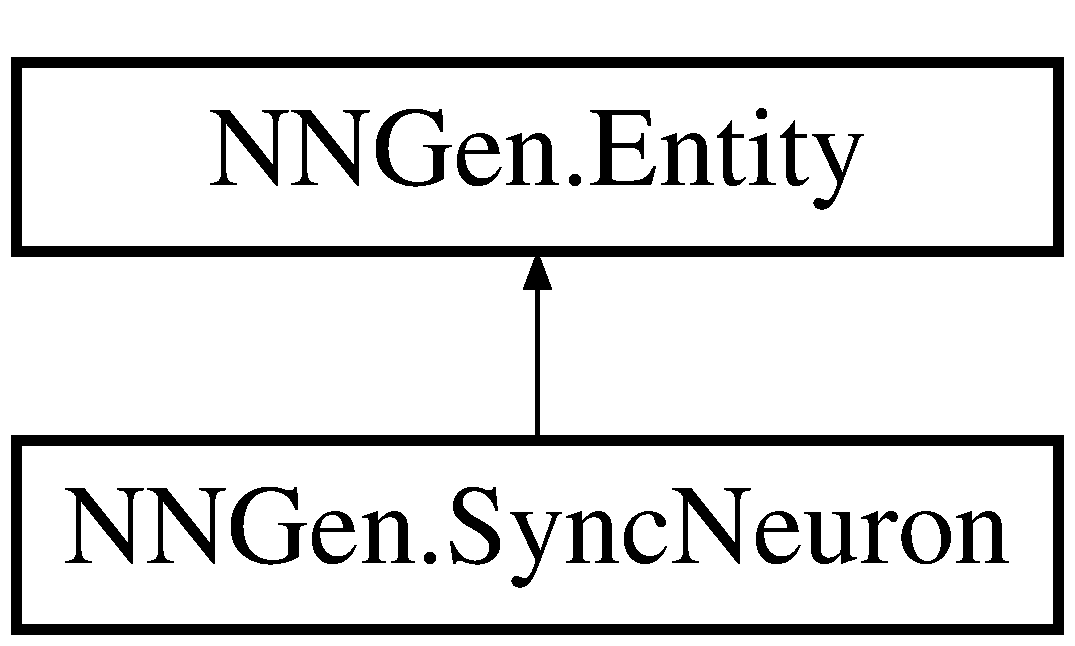
\includegraphics[height=2.000000cm]{class_n_n_gen_1_1_sync_neuron}
\end{center}
\end{figure}
\subsection*{Public Member Functions}
\begin{DoxyCompactItemize}
\item 
\hyperlink{class_n_n_gen_1_1_sync_neuron_a500526443c9e0009cc7aa9f678795bfb}{Sync\+Neuron} (\hyperlink{class_n_n_gen_1_1_port}{Port}\mbox{[}$\,$\mbox{]} \+\_\+input\+Ports, int \+\_\+num\+Output\+Int\+Bits, int \+\_\+num\+Output\+Frac\+Bits, int \+\_\+num\+Weight\+Int\+Bits, string \+\_\+name)
\begin{DoxyCompactList}\small\item\em Create a synchronous neuron \end{DoxyCompactList}\item 
override string \hyperlink{class_n_n_gen_1_1_sync_neuron_a0d24dc5f802b28e58318bbc70e4e999a}{get\+Name} ()
\begin{DoxyCompactList}\small\item\em Returns the name of the neuron \end{DoxyCompactList}\item 
override \hyperlink{class_n_n_gen_1_1_port}{Port}\mbox{[}$\,$\mbox{]} \hyperlink{class_n_n_gen_1_1_sync_neuron_a9f391d4a186cdd79f97ece5adab9ff6c}{get\+Input\+Ports} ()
\begin{DoxyCompactList}\small\item\em Returns the input ports to the neuron \end{DoxyCompactList}\item 
override \hyperlink{class_n_n_gen_1_1_port}{Port}\mbox{[}$\,$\mbox{]} \hyperlink{class_n_n_gen_1_1_sync_neuron_a79f19432c86cbaf3a2eaa2090cecf9cf}{get\+Output\+Ports} ()
\begin{DoxyCompactList}\small\item\em Returns the output ports of the neuron \end{DoxyCompactList}\item 
override \hyperlink{class_n_n_gen_1_1_signal}{Signal}\mbox{[}$\,$\mbox{]} \hyperlink{class_n_n_gen_1_1_sync_neuron_a615a906839d1227ca0e4605b4165f892}{get\+Internal\+Signals} ()
\begin{DoxyCompactList}\small\item\em Returns a list of internal signals for the neuron \end{DoxyCompactList}\item 
override bool \hyperlink{class_n_n_gen_1_1_sync_neuron_aebc20821885a0661e98403b4a7722643}{write\+V\+H\+D\+L} (string file\+Path)
\begin{DoxyCompactList}\small\item\em Writes the .vhd file that describes the neuron. \end{DoxyCompactList}\end{DoxyCompactItemize}
\subsection*{Properties}
\begin{DoxyCompactItemize}
\item 
\hyperlink{class_n_n_gen_1_1_port}{Port}\mbox{[}$\,$\mbox{]} \hyperlink{class_n_n_gen_1_1_sync_neuron_a717f010aa22ec2a35ec0f314549a3177}{neuron\+Inputs}\hspace{0.3cm}{\ttfamily  \mbox{[}get\mbox{]}}
\begin{DoxyCompactList}\small\item\em The inputs to the neuron \end{DoxyCompactList}\item 
\hyperlink{class_n_n_gen_1_1_port}{Port} \hyperlink{class_n_n_gen_1_1_sync_neuron_a0124d151cc6e1ff3dfbfe917e4d0ab2f}{neuron\+Output}\hspace{0.3cm}{\ttfamily  \mbox{[}get\mbox{]}}
\begin{DoxyCompactList}\small\item\em The output to the neuron \end{DoxyCompactList}\item 
\hyperlink{class_n_n_gen_1_1_port}{Port} \hyperlink{class_n_n_gen_1_1_sync_neuron_ac05c041707c4ede2fd412b9ea7a9bb08}{clk}\hspace{0.3cm}{\ttfamily  \mbox{[}get\mbox{]}}
\begin{DoxyCompactList}\small\item\em The neuron\textquotesingle{}s clock signal. Used for both loading and computing \end{DoxyCompactList}\item 
\hyperlink{class_n_n_gen_1_1_port}{Port} \hyperlink{class_n_n_gen_1_1_sync_neuron_a6aec644cafdc8c9f4d03515e3c0e7b0b}{Activate}\hspace{0.3cm}{\ttfamily  \mbox{[}get\mbox{]}}
\begin{DoxyCompactList}\small\item\em When high, the neuron will continue the computation process. When low, it will pause. \end{DoxyCompactList}\item 
\hyperlink{class_n_n_gen_1_1_port}{Port} \hyperlink{class_n_n_gen_1_1_sync_neuron_a5cb034f95e9d284d3638f9e817c3f26f}{load\+Enable}\hspace{0.3cm}{\ttfamily  \mbox{[}get\mbox{]}}
\begin{DoxyCompactList}\small\item\em When high, the neuron will continue the weight loading process. When low, it will pause the load process. \end{DoxyCompactList}\item 
\hyperlink{class_n_n_gen_1_1_port}{Port} \hyperlink{class_n_n_gen_1_1_sync_neuron_a4334c7219b366b989108a9451ff3c409}{load\+Value}\hspace{0.3cm}{\ttfamily  \mbox{[}get\mbox{]}}
\begin{DoxyCompactList}\small\item\em The value to load into the weight signal indexed by load\+Offset \end{DoxyCompactList}\item 
\hyperlink{class_n_n_gen_1_1_port}{Port} \hyperlink{class_n_n_gen_1_1_sync_neuron_a1ad5ac56ac0278154e84eeeb4ae09604}{load\+Offset}\hspace{0.3cm}{\ttfamily  \mbox{[}get\mbox{]}}
\begin{DoxyCompactList}\small\item\em The offset at which to load load\+Value into the weight signals \end{DoxyCompactList}\item 
\hyperlink{class_n_n_gen_1_1_port}{Port} \hyperlink{class_n_n_gen_1_1_sync_neuron_a871ce93f3b672a3425fec4ee5d55a5d5}{final\+Load}\hspace{0.3cm}{\ttfamily  \mbox{[}get\mbox{]}}
\begin{DoxyCompactList}\small\item\em When high, the final weight signal has been loaded \end{DoxyCompactList}\item 
\hyperlink{class_n_n_gen_1_1_signal}{Signal}\mbox{[}$\,$\mbox{]} \hyperlink{class_n_n_gen_1_1_sync_neuron_a1d9363beee9303179a0f47c0f143f97a}{weight\+Signals}\hspace{0.3cm}{\ttfamily  \mbox{[}get\mbox{]}}
\begin{DoxyCompactList}\small\item\em The weights of each of the individual inputs \end{DoxyCompactList}\item 
\hyperlink{class_n_n_gen_1_1_signal}{Signal} \hyperlink{class_n_n_gen_1_1_sync_neuron_a7903497d879961c468b41d704fc6e110}{clock\+Iter}\hspace{0.3cm}{\ttfamily  \mbox{[}get\mbox{]}}
\begin{DoxyCompactList}\small\item\em A signal used to count the number of clocks that have elapsed \end{DoxyCompactList}\item 
\hyperlink{class_n_n_gen_1_1_signal}{Signal} \hyperlink{class_n_n_gen_1_1_sync_neuron_a3eb9c8d040a716f504bfb373bc17eabf}{current\+Product}\hspace{0.3cm}{\ttfamily  \mbox{[}get\mbox{]}}
\begin{DoxyCompactList}\small\item\em Holds the current product of a weight and an input \end{DoxyCompactList}\item 
\hyperlink{class_n_n_gen_1_1_signal}{Signal} \hyperlink{class_n_n_gen_1_1_sync_neuron_a5414c6e7b74fc581c53f4a5a5ec8bd21}{current\+Sum}\hspace{0.3cm}{\ttfamily  \mbox{[}get\mbox{]}}
\begin{DoxyCompactList}\small\item\em Holds the sum of current\+Product and the cumulative sum of the previous states of current\+Product \end{DoxyCompactList}\item 
\hyperlink{class_n_n_gen_1_1_signal}{Signal} \hyperlink{class_n_n_gen_1_1_sync_neuron_a025ec7f0da6e80d24e55f23e939afcec}{sum}\hspace{0.3cm}{\ttfamily  \mbox{[}get\mbox{]}}
\begin{DoxyCompactList}\small\item\em Holds the cumulative sum of the states of current\+Product \end{DoxyCompactList}\item 
\hyperlink{class_n_n_gen_1_1_signal}{Signal} \hyperlink{class_n_n_gen_1_1_sync_neuron_ac80f32363948c3482290c24ef800fb8d}{latch\+Out}\hspace{0.3cm}{\ttfamily  \mbox{[}get\mbox{]}}
\begin{DoxyCompactList}\small\item\em A latch so the output doesn\textquotesingle{}t fluctuate while being computed \end{DoxyCompactList}\item 
string \hyperlink{class_n_n_gen_1_1_sync_neuron_a52bca099e4e4dca870213d0bdc0a734d}{name}\hspace{0.3cm}{\ttfamily  \mbox{[}get\mbox{]}}
\begin{DoxyCompactList}\small\item\em The name of the neuron \end{DoxyCompactList}\end{DoxyCompactItemize}


\subsection{Detailed Description}
A class representing a singular neuron in a synchronous neural network 



\subsection{Constructor \& Destructor Documentation}
\hypertarget{class_n_n_gen_1_1_sync_neuron_a500526443c9e0009cc7aa9f678795bfb}{}\index{N\+N\+Gen\+::\+Sync\+Neuron@{N\+N\+Gen\+::\+Sync\+Neuron}!Sync\+Neuron@{Sync\+Neuron}}
\index{Sync\+Neuron@{Sync\+Neuron}!N\+N\+Gen\+::\+Sync\+Neuron@{N\+N\+Gen\+::\+Sync\+Neuron}}
\subsubsection[{Sync\+Neuron(\+Port[] \+\_\+input\+Ports, int \+\_\+num\+Output\+Int\+Bits, int \+\_\+num\+Output\+Frac\+Bits, int \+\_\+num\+Weight\+Int\+Bits, string \+\_\+name)}]{\setlength{\rightskip}{0pt plus 5cm}N\+N\+Gen.\+Sync\+Neuron.\+Sync\+Neuron (
\begin{DoxyParamCaption}
\item[{{\bf Port}\mbox{[}$\,$\mbox{]}}]{\+\_\+input\+Ports, }
\item[{int}]{\+\_\+num\+Output\+Int\+Bits, }
\item[{int}]{\+\_\+num\+Output\+Frac\+Bits, }
\item[{int}]{\+\_\+num\+Weight\+Int\+Bits, }
\item[{string}]{\+\_\+name}
\end{DoxyParamCaption}
)\hspace{0.3cm}{\ttfamily [inline]}}\label{class_n_n_gen_1_1_sync_neuron_a500526443c9e0009cc7aa9f678795bfb}


Create a synchronous neuron 


\begin{DoxyParams}{Parameters}
{\em \+\_\+input\+Ports} & The inputs to the network\\
\hline
{\em \+\_\+num\+Output\+Int\+Bits} & The number of output integer bits from the neuron\\
\hline
{\em \+\_\+num\+Output\+Frac\+Bits} & The number of output fractional bits from the neuron\\
\hline
{\em \+\_\+num\+Weight\+Int\+Bits} & The number of integer bits to use in the weight signals\\
\hline
{\em \+\_\+name} & The name of the neuron\\
\hline
\end{DoxyParams}


\subsection{Member Function Documentation}
\hypertarget{class_n_n_gen_1_1_sync_neuron_a9f391d4a186cdd79f97ece5adab9ff6c}{}\index{N\+N\+Gen\+::\+Sync\+Neuron@{N\+N\+Gen\+::\+Sync\+Neuron}!get\+Input\+Ports@{get\+Input\+Ports}}
\index{get\+Input\+Ports@{get\+Input\+Ports}!N\+N\+Gen\+::\+Sync\+Neuron@{N\+N\+Gen\+::\+Sync\+Neuron}}
\subsubsection[{get\+Input\+Ports()}]{\setlength{\rightskip}{0pt plus 5cm}override {\bf Port} \mbox{[}$\,$\mbox{]} N\+N\+Gen.\+Sync\+Neuron.\+get\+Input\+Ports (
\begin{DoxyParamCaption}
{}
\end{DoxyParamCaption}
)\hspace{0.3cm}{\ttfamily [inline]}, {\ttfamily [virtual]}}\label{class_n_n_gen_1_1_sync_neuron_a9f391d4a186cdd79f97ece5adab9ff6c}


Returns the input ports to the neuron 

\begin{DoxyReturn}{Returns}
The input ports to the neuron
\end{DoxyReturn}


Implements \hyperlink{class_n_n_gen_1_1_entity_a01239f05c9efa61ec9e6a29cb2eaad50}{N\+N\+Gen.\+Entity}.

\hypertarget{class_n_n_gen_1_1_sync_neuron_a615a906839d1227ca0e4605b4165f892}{}\index{N\+N\+Gen\+::\+Sync\+Neuron@{N\+N\+Gen\+::\+Sync\+Neuron}!get\+Internal\+Signals@{get\+Internal\+Signals}}
\index{get\+Internal\+Signals@{get\+Internal\+Signals}!N\+N\+Gen\+::\+Sync\+Neuron@{N\+N\+Gen\+::\+Sync\+Neuron}}
\subsubsection[{get\+Internal\+Signals()}]{\setlength{\rightskip}{0pt plus 5cm}override {\bf Signal} \mbox{[}$\,$\mbox{]} N\+N\+Gen.\+Sync\+Neuron.\+get\+Internal\+Signals (
\begin{DoxyParamCaption}
{}
\end{DoxyParamCaption}
)\hspace{0.3cm}{\ttfamily [inline]}, {\ttfamily [virtual]}}\label{class_n_n_gen_1_1_sync_neuron_a615a906839d1227ca0e4605b4165f892}


Returns a list of internal signals for the neuron 

\begin{DoxyReturn}{Returns}
The internal signals for the neuron
\end{DoxyReturn}


Implements \hyperlink{class_n_n_gen_1_1_entity_a62feb80e95ec84c650ea17bd53f0d510}{N\+N\+Gen.\+Entity}.

\hypertarget{class_n_n_gen_1_1_sync_neuron_a0d24dc5f802b28e58318bbc70e4e999a}{}\index{N\+N\+Gen\+::\+Sync\+Neuron@{N\+N\+Gen\+::\+Sync\+Neuron}!get\+Name@{get\+Name}}
\index{get\+Name@{get\+Name}!N\+N\+Gen\+::\+Sync\+Neuron@{N\+N\+Gen\+::\+Sync\+Neuron}}
\subsubsection[{get\+Name()}]{\setlength{\rightskip}{0pt plus 5cm}override string N\+N\+Gen.\+Sync\+Neuron.\+get\+Name (
\begin{DoxyParamCaption}
{}
\end{DoxyParamCaption}
)\hspace{0.3cm}{\ttfamily [inline]}, {\ttfamily [virtual]}}\label{class_n_n_gen_1_1_sync_neuron_a0d24dc5f802b28e58318bbc70e4e999a}


Returns the name of the neuron 

\begin{DoxyReturn}{Returns}
The name of the neuron
\end{DoxyReturn}


Implements \hyperlink{class_n_n_gen_1_1_entity_a9f25d1070c9ab8ad343c28443e62e6f2}{N\+N\+Gen.\+Entity}.

\hypertarget{class_n_n_gen_1_1_sync_neuron_a79f19432c86cbaf3a2eaa2090cecf9cf}{}\index{N\+N\+Gen\+::\+Sync\+Neuron@{N\+N\+Gen\+::\+Sync\+Neuron}!get\+Output\+Ports@{get\+Output\+Ports}}
\index{get\+Output\+Ports@{get\+Output\+Ports}!N\+N\+Gen\+::\+Sync\+Neuron@{N\+N\+Gen\+::\+Sync\+Neuron}}
\subsubsection[{get\+Output\+Ports()}]{\setlength{\rightskip}{0pt plus 5cm}override {\bf Port} \mbox{[}$\,$\mbox{]} N\+N\+Gen.\+Sync\+Neuron.\+get\+Output\+Ports (
\begin{DoxyParamCaption}
{}
\end{DoxyParamCaption}
)\hspace{0.3cm}{\ttfamily [inline]}, {\ttfamily [virtual]}}\label{class_n_n_gen_1_1_sync_neuron_a79f19432c86cbaf3a2eaa2090cecf9cf}


Returns the output ports of the neuron 

\begin{DoxyReturn}{Returns}
The output ports of the neuron
\end{DoxyReturn}


Implements \hyperlink{class_n_n_gen_1_1_entity_ace06368087778e254a5048c7d28747be}{N\+N\+Gen.\+Entity}.

\hypertarget{class_n_n_gen_1_1_sync_neuron_aebc20821885a0661e98403b4a7722643}{}\index{N\+N\+Gen\+::\+Sync\+Neuron@{N\+N\+Gen\+::\+Sync\+Neuron}!write\+V\+H\+D\+L@{write\+V\+H\+D\+L}}
\index{write\+V\+H\+D\+L@{write\+V\+H\+D\+L}!N\+N\+Gen\+::\+Sync\+Neuron@{N\+N\+Gen\+::\+Sync\+Neuron}}
\subsubsection[{write\+V\+H\+D\+L(string file\+Path)}]{\setlength{\rightskip}{0pt plus 5cm}override bool N\+N\+Gen.\+Sync\+Neuron.\+write\+V\+H\+D\+L (
\begin{DoxyParamCaption}
\item[{string}]{file\+Path}
\end{DoxyParamCaption}
)\hspace{0.3cm}{\ttfamily [inline]}, {\ttfamily [virtual]}}\label{class_n_n_gen_1_1_sync_neuron_aebc20821885a0661e98403b4a7722643}


Writes the .vhd file that describes the neuron. 


\begin{DoxyParams}{Parameters}
{\em file\+Path} & The root file path for the network. Do not include \char`\"{}(name).\+vhd\char`\"{} in the filepath\\
\hline
\end{DoxyParams}
\begin{DoxyReturn}{Returns}
True if the file was written successfully, false otherwise
\end{DoxyReturn}


Implements \hyperlink{class_n_n_gen_1_1_entity_a1111d498446be08b20583b9625893a52}{N\+N\+Gen.\+Entity}.



\subsection{Property Documentation}
\hypertarget{class_n_n_gen_1_1_sync_neuron_a6aec644cafdc8c9f4d03515e3c0e7b0b}{}\index{N\+N\+Gen\+::\+Sync\+Neuron@{N\+N\+Gen\+::\+Sync\+Neuron}!Activate@{Activate}}
\index{Activate@{Activate}!N\+N\+Gen\+::\+Sync\+Neuron@{N\+N\+Gen\+::\+Sync\+Neuron}}
\subsubsection[{Activate}]{\setlength{\rightskip}{0pt plus 5cm}{\bf Port} N\+N\+Gen.\+Sync\+Neuron.\+Activate\hspace{0.3cm}{\ttfamily [get]}}\label{class_n_n_gen_1_1_sync_neuron_a6aec644cafdc8c9f4d03515e3c0e7b0b}


When high, the neuron will continue the computation process. When low, it will pause. 

\hypertarget{class_n_n_gen_1_1_sync_neuron_ac05c041707c4ede2fd412b9ea7a9bb08}{}\index{N\+N\+Gen\+::\+Sync\+Neuron@{N\+N\+Gen\+::\+Sync\+Neuron}!clk@{clk}}
\index{clk@{clk}!N\+N\+Gen\+::\+Sync\+Neuron@{N\+N\+Gen\+::\+Sync\+Neuron}}
\subsubsection[{clk}]{\setlength{\rightskip}{0pt plus 5cm}{\bf Port} N\+N\+Gen.\+Sync\+Neuron.\+clk\hspace{0.3cm}{\ttfamily [get]}}\label{class_n_n_gen_1_1_sync_neuron_ac05c041707c4ede2fd412b9ea7a9bb08}


The neuron\textquotesingle{}s clock signal. Used for both loading and computing 

\hypertarget{class_n_n_gen_1_1_sync_neuron_a7903497d879961c468b41d704fc6e110}{}\index{N\+N\+Gen\+::\+Sync\+Neuron@{N\+N\+Gen\+::\+Sync\+Neuron}!clock\+Iter@{clock\+Iter}}
\index{clock\+Iter@{clock\+Iter}!N\+N\+Gen\+::\+Sync\+Neuron@{N\+N\+Gen\+::\+Sync\+Neuron}}
\subsubsection[{clock\+Iter}]{\setlength{\rightskip}{0pt plus 5cm}{\bf Signal} N\+N\+Gen.\+Sync\+Neuron.\+clock\+Iter\hspace{0.3cm}{\ttfamily [get]}}\label{class_n_n_gen_1_1_sync_neuron_a7903497d879961c468b41d704fc6e110}


A signal used to count the number of clocks that have elapsed 

\hypertarget{class_n_n_gen_1_1_sync_neuron_a3eb9c8d040a716f504bfb373bc17eabf}{}\index{N\+N\+Gen\+::\+Sync\+Neuron@{N\+N\+Gen\+::\+Sync\+Neuron}!current\+Product@{current\+Product}}
\index{current\+Product@{current\+Product}!N\+N\+Gen\+::\+Sync\+Neuron@{N\+N\+Gen\+::\+Sync\+Neuron}}
\subsubsection[{current\+Product}]{\setlength{\rightskip}{0pt plus 5cm}{\bf Signal} N\+N\+Gen.\+Sync\+Neuron.\+current\+Product\hspace{0.3cm}{\ttfamily [get]}}\label{class_n_n_gen_1_1_sync_neuron_a3eb9c8d040a716f504bfb373bc17eabf}


Holds the current product of a weight and an input 

\hypertarget{class_n_n_gen_1_1_sync_neuron_a5414c6e7b74fc581c53f4a5a5ec8bd21}{}\index{N\+N\+Gen\+::\+Sync\+Neuron@{N\+N\+Gen\+::\+Sync\+Neuron}!current\+Sum@{current\+Sum}}
\index{current\+Sum@{current\+Sum}!N\+N\+Gen\+::\+Sync\+Neuron@{N\+N\+Gen\+::\+Sync\+Neuron}}
\subsubsection[{current\+Sum}]{\setlength{\rightskip}{0pt plus 5cm}{\bf Signal} N\+N\+Gen.\+Sync\+Neuron.\+current\+Sum\hspace{0.3cm}{\ttfamily [get]}}\label{class_n_n_gen_1_1_sync_neuron_a5414c6e7b74fc581c53f4a5a5ec8bd21}


Holds the sum of current\+Product and the cumulative sum of the previous states of current\+Product 

\hypertarget{class_n_n_gen_1_1_sync_neuron_a871ce93f3b672a3425fec4ee5d55a5d5}{}\index{N\+N\+Gen\+::\+Sync\+Neuron@{N\+N\+Gen\+::\+Sync\+Neuron}!final\+Load@{final\+Load}}
\index{final\+Load@{final\+Load}!N\+N\+Gen\+::\+Sync\+Neuron@{N\+N\+Gen\+::\+Sync\+Neuron}}
\subsubsection[{final\+Load}]{\setlength{\rightskip}{0pt plus 5cm}{\bf Port} N\+N\+Gen.\+Sync\+Neuron.\+final\+Load\hspace{0.3cm}{\ttfamily [get]}}\label{class_n_n_gen_1_1_sync_neuron_a871ce93f3b672a3425fec4ee5d55a5d5}


When high, the final weight signal has been loaded 

\hypertarget{class_n_n_gen_1_1_sync_neuron_ac80f32363948c3482290c24ef800fb8d}{}\index{N\+N\+Gen\+::\+Sync\+Neuron@{N\+N\+Gen\+::\+Sync\+Neuron}!latch\+Out@{latch\+Out}}
\index{latch\+Out@{latch\+Out}!N\+N\+Gen\+::\+Sync\+Neuron@{N\+N\+Gen\+::\+Sync\+Neuron}}
\subsubsection[{latch\+Out}]{\setlength{\rightskip}{0pt plus 5cm}{\bf Signal} N\+N\+Gen.\+Sync\+Neuron.\+latch\+Out\hspace{0.3cm}{\ttfamily [get]}}\label{class_n_n_gen_1_1_sync_neuron_ac80f32363948c3482290c24ef800fb8d}


A latch so the output doesn\textquotesingle{}t fluctuate while being computed 

\hypertarget{class_n_n_gen_1_1_sync_neuron_a5cb034f95e9d284d3638f9e817c3f26f}{}\index{N\+N\+Gen\+::\+Sync\+Neuron@{N\+N\+Gen\+::\+Sync\+Neuron}!load\+Enable@{load\+Enable}}
\index{load\+Enable@{load\+Enable}!N\+N\+Gen\+::\+Sync\+Neuron@{N\+N\+Gen\+::\+Sync\+Neuron}}
\subsubsection[{load\+Enable}]{\setlength{\rightskip}{0pt plus 5cm}{\bf Port} N\+N\+Gen.\+Sync\+Neuron.\+load\+Enable\hspace{0.3cm}{\ttfamily [get]}}\label{class_n_n_gen_1_1_sync_neuron_a5cb034f95e9d284d3638f9e817c3f26f}


When high, the neuron will continue the weight loading process. When low, it will pause the load process. 

\hypertarget{class_n_n_gen_1_1_sync_neuron_a1ad5ac56ac0278154e84eeeb4ae09604}{}\index{N\+N\+Gen\+::\+Sync\+Neuron@{N\+N\+Gen\+::\+Sync\+Neuron}!load\+Offset@{load\+Offset}}
\index{load\+Offset@{load\+Offset}!N\+N\+Gen\+::\+Sync\+Neuron@{N\+N\+Gen\+::\+Sync\+Neuron}}
\subsubsection[{load\+Offset}]{\setlength{\rightskip}{0pt plus 5cm}{\bf Port} N\+N\+Gen.\+Sync\+Neuron.\+load\+Offset\hspace{0.3cm}{\ttfamily [get]}}\label{class_n_n_gen_1_1_sync_neuron_a1ad5ac56ac0278154e84eeeb4ae09604}


The offset at which to load load\+Value into the weight signals 

\hypertarget{class_n_n_gen_1_1_sync_neuron_a4334c7219b366b989108a9451ff3c409}{}\index{N\+N\+Gen\+::\+Sync\+Neuron@{N\+N\+Gen\+::\+Sync\+Neuron}!load\+Value@{load\+Value}}
\index{load\+Value@{load\+Value}!N\+N\+Gen\+::\+Sync\+Neuron@{N\+N\+Gen\+::\+Sync\+Neuron}}
\subsubsection[{load\+Value}]{\setlength{\rightskip}{0pt plus 5cm}{\bf Port} N\+N\+Gen.\+Sync\+Neuron.\+load\+Value\hspace{0.3cm}{\ttfamily [get]}}\label{class_n_n_gen_1_1_sync_neuron_a4334c7219b366b989108a9451ff3c409}


The value to load into the weight signal indexed by load\+Offset 

\hypertarget{class_n_n_gen_1_1_sync_neuron_a52bca099e4e4dca870213d0bdc0a734d}{}\index{N\+N\+Gen\+::\+Sync\+Neuron@{N\+N\+Gen\+::\+Sync\+Neuron}!name@{name}}
\index{name@{name}!N\+N\+Gen\+::\+Sync\+Neuron@{N\+N\+Gen\+::\+Sync\+Neuron}}
\subsubsection[{name}]{\setlength{\rightskip}{0pt plus 5cm}string N\+N\+Gen.\+Sync\+Neuron.\+name\hspace{0.3cm}{\ttfamily [get]}}\label{class_n_n_gen_1_1_sync_neuron_a52bca099e4e4dca870213d0bdc0a734d}


The name of the neuron 

\hypertarget{class_n_n_gen_1_1_sync_neuron_a717f010aa22ec2a35ec0f314549a3177}{}\index{N\+N\+Gen\+::\+Sync\+Neuron@{N\+N\+Gen\+::\+Sync\+Neuron}!neuron\+Inputs@{neuron\+Inputs}}
\index{neuron\+Inputs@{neuron\+Inputs}!N\+N\+Gen\+::\+Sync\+Neuron@{N\+N\+Gen\+::\+Sync\+Neuron}}
\subsubsection[{neuron\+Inputs}]{\setlength{\rightskip}{0pt plus 5cm}{\bf Port} \mbox{[}$\,$\mbox{]} N\+N\+Gen.\+Sync\+Neuron.\+neuron\+Inputs\hspace{0.3cm}{\ttfamily [get]}}\label{class_n_n_gen_1_1_sync_neuron_a717f010aa22ec2a35ec0f314549a3177}


The inputs to the neuron 

\hypertarget{class_n_n_gen_1_1_sync_neuron_a0124d151cc6e1ff3dfbfe917e4d0ab2f}{}\index{N\+N\+Gen\+::\+Sync\+Neuron@{N\+N\+Gen\+::\+Sync\+Neuron}!neuron\+Output@{neuron\+Output}}
\index{neuron\+Output@{neuron\+Output}!N\+N\+Gen\+::\+Sync\+Neuron@{N\+N\+Gen\+::\+Sync\+Neuron}}
\subsubsection[{neuron\+Output}]{\setlength{\rightskip}{0pt plus 5cm}{\bf Port} N\+N\+Gen.\+Sync\+Neuron.\+neuron\+Output\hspace{0.3cm}{\ttfamily [get]}}\label{class_n_n_gen_1_1_sync_neuron_a0124d151cc6e1ff3dfbfe917e4d0ab2f}


The output to the neuron 

\hypertarget{class_n_n_gen_1_1_sync_neuron_a025ec7f0da6e80d24e55f23e939afcec}{}\index{N\+N\+Gen\+::\+Sync\+Neuron@{N\+N\+Gen\+::\+Sync\+Neuron}!sum@{sum}}
\index{sum@{sum}!N\+N\+Gen\+::\+Sync\+Neuron@{N\+N\+Gen\+::\+Sync\+Neuron}}
\subsubsection[{sum}]{\setlength{\rightskip}{0pt plus 5cm}{\bf Signal} N\+N\+Gen.\+Sync\+Neuron.\+sum\hspace{0.3cm}{\ttfamily [get]}}\label{class_n_n_gen_1_1_sync_neuron_a025ec7f0da6e80d24e55f23e939afcec}


Holds the cumulative sum of the states of current\+Product 

\hypertarget{class_n_n_gen_1_1_sync_neuron_a1d9363beee9303179a0f47c0f143f97a}{}\index{N\+N\+Gen\+::\+Sync\+Neuron@{N\+N\+Gen\+::\+Sync\+Neuron}!weight\+Signals@{weight\+Signals}}
\index{weight\+Signals@{weight\+Signals}!N\+N\+Gen\+::\+Sync\+Neuron@{N\+N\+Gen\+::\+Sync\+Neuron}}
\subsubsection[{weight\+Signals}]{\setlength{\rightskip}{0pt plus 5cm}{\bf Signal} \mbox{[}$\,$\mbox{]} N\+N\+Gen.\+Sync\+Neuron.\+weight\+Signals\hspace{0.3cm}{\ttfamily [get]}}\label{class_n_n_gen_1_1_sync_neuron_a1d9363beee9303179a0f47c0f143f97a}


The weights of each of the individual inputs 



The documentation for this class was generated from the following file\+:\begin{DoxyCompactItemize}
\item 
E\+:/\+Documents/\+Visual Studio 2013/\+Projects/\+Neural\+Network/\+N\+N\+Gen/\hyperlink{_sync_neuron_8cs}{Sync\+Neuron.\+cs}\end{DoxyCompactItemize}

\hypertarget{class_n_n_gen_1_1_sync_or_async}{}\section{N\+N\+Gen.\+Sync\+Or\+Async Class Reference}
\label{class_n_n_gen_1_1_sync_or_async}\index{N\+N\+Gen.\+Sync\+Or\+Async@{N\+N\+Gen.\+Sync\+Or\+Async}}


A U\+I element allowing the user to set whether the network is synchronous or asynchronous  


Inheritance diagram for N\+N\+Gen.\+Sync\+Or\+Async\+:\begin{figure}[H]
\begin{center}
\leavevmode
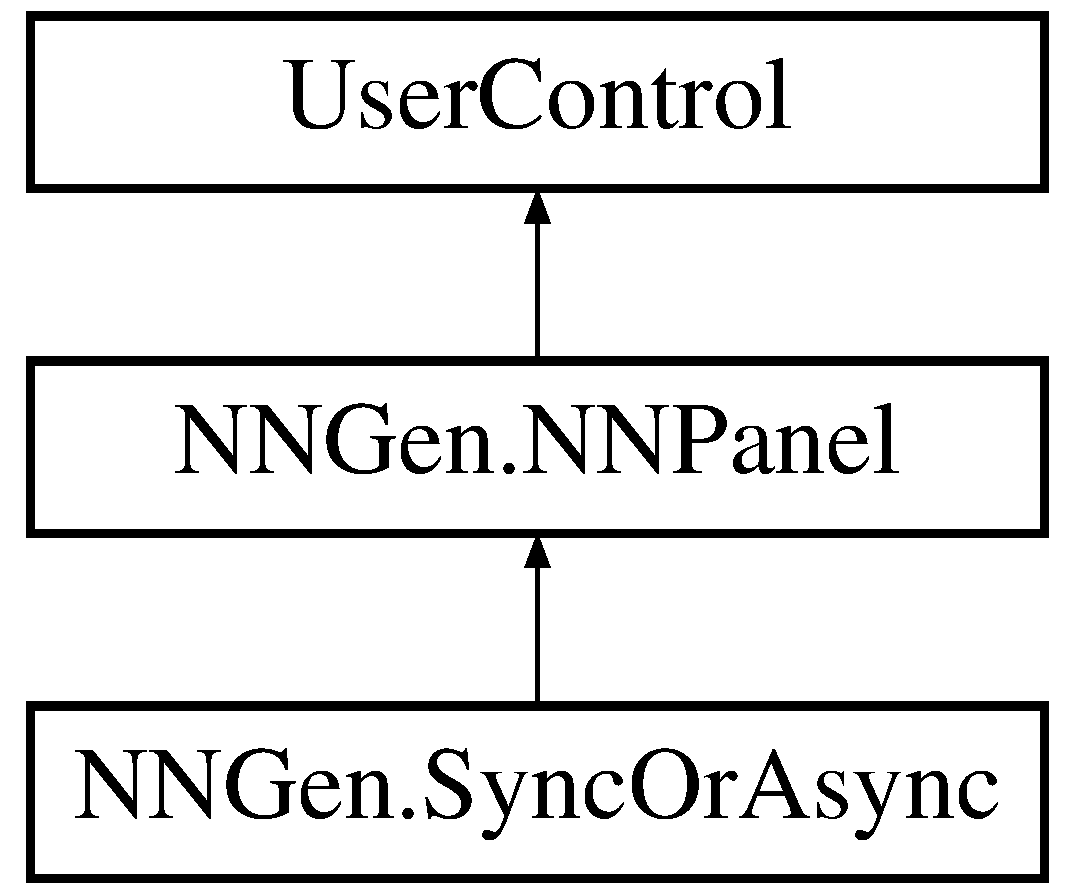
\includegraphics[height=3.000000cm]{class_n_n_gen_1_1_sync_or_async}
\end{center}
\end{figure}
\subsection*{Public Member Functions}
\begin{DoxyCompactItemize}
\item 
\hyperlink{class_n_n_gen_1_1_sync_or_async_a39ad84feadeb6aa5f66a932c6679f4e3}{Sync\+Or\+Async} ()
\begin{DoxyCompactList}\small\item\em Initialize the form \end{DoxyCompactList}\item 
override bool \hyperlink{class_n_n_gen_1_1_sync_or_async_a43e1723039a0485fe09f6f374eb48620}{verify} ()
\begin{DoxyCompactList}\small\item\em The \hyperlink{class_n_n_gen_1_1_sync_or_async_a43e1723039a0485fe09f6f374eb48620}{verify()} method implementation for this class. See N\+N\+Pannel.\+verify() for more documentation. \end{DoxyCompactList}\item 
bool \hyperlink{class_n_n_gen_1_1_sync_or_async_ad9f608f2c61cc51ad7abc68961bfffb1}{is\+Synchronous\+Network} ()
\begin{DoxyCompactList}\small\item\em Determines whether the user has specified that the network is synchronous or asynchronous \end{DoxyCompactList}\end{DoxyCompactItemize}
\subsection*{Protected Member Functions}
\begin{DoxyCompactItemize}
\item 
override void \hyperlink{class_n_n_gen_1_1_sync_or_async_ae983c7668dca65753d841767495a299a}{Dispose} (bool disposing)
\begin{DoxyCompactList}\small\item\em Clean up any resources being used. \end{DoxyCompactList}\end{DoxyCompactItemize}


\subsection{Detailed Description}
A U\+I element allowing the user to set whether the network is synchronous or asynchronous 



\subsection{Constructor \& Destructor Documentation}
\hypertarget{class_n_n_gen_1_1_sync_or_async_a39ad84feadeb6aa5f66a932c6679f4e3}{}\index{N\+N\+Gen\+::\+Sync\+Or\+Async@{N\+N\+Gen\+::\+Sync\+Or\+Async}!Sync\+Or\+Async@{Sync\+Or\+Async}}
\index{Sync\+Or\+Async@{Sync\+Or\+Async}!N\+N\+Gen\+::\+Sync\+Or\+Async@{N\+N\+Gen\+::\+Sync\+Or\+Async}}
\subsubsection[{Sync\+Or\+Async()}]{\setlength{\rightskip}{0pt plus 5cm}N\+N\+Gen.\+Sync\+Or\+Async.\+Sync\+Or\+Async (
\begin{DoxyParamCaption}
{}
\end{DoxyParamCaption}
)\hspace{0.3cm}{\ttfamily [inline]}}\label{class_n_n_gen_1_1_sync_or_async_a39ad84feadeb6aa5f66a932c6679f4e3}


Initialize the form 



\subsection{Member Function Documentation}
\hypertarget{class_n_n_gen_1_1_sync_or_async_ae983c7668dca65753d841767495a299a}{}\index{N\+N\+Gen\+::\+Sync\+Or\+Async@{N\+N\+Gen\+::\+Sync\+Or\+Async}!Dispose@{Dispose}}
\index{Dispose@{Dispose}!N\+N\+Gen\+::\+Sync\+Or\+Async@{N\+N\+Gen\+::\+Sync\+Or\+Async}}
\subsubsection[{Dispose(bool disposing)}]{\setlength{\rightskip}{0pt plus 5cm}override void N\+N\+Gen.\+Sync\+Or\+Async.\+Dispose (
\begin{DoxyParamCaption}
\item[{bool}]{disposing}
\end{DoxyParamCaption}
)\hspace{0.3cm}{\ttfamily [inline]}, {\ttfamily [protected]}}\label{class_n_n_gen_1_1_sync_or_async_ae983c7668dca65753d841767495a299a}


Clean up any resources being used. 


\begin{DoxyParams}{Parameters}
{\em disposing} & true if managed resources should be disposed; otherwise, false.\\
\hline
\end{DoxyParams}
\hypertarget{class_n_n_gen_1_1_sync_or_async_ad9f608f2c61cc51ad7abc68961bfffb1}{}\index{N\+N\+Gen\+::\+Sync\+Or\+Async@{N\+N\+Gen\+::\+Sync\+Or\+Async}!is\+Synchronous\+Network@{is\+Synchronous\+Network}}
\index{is\+Synchronous\+Network@{is\+Synchronous\+Network}!N\+N\+Gen\+::\+Sync\+Or\+Async@{N\+N\+Gen\+::\+Sync\+Or\+Async}}
\subsubsection[{is\+Synchronous\+Network()}]{\setlength{\rightskip}{0pt plus 5cm}bool N\+N\+Gen.\+Sync\+Or\+Async.\+is\+Synchronous\+Network (
\begin{DoxyParamCaption}
{}
\end{DoxyParamCaption}
)\hspace{0.3cm}{\ttfamily [inline]}}\label{class_n_n_gen_1_1_sync_or_async_ad9f608f2c61cc51ad7abc68961bfffb1}


Determines whether the user has specified that the network is synchronous or asynchronous 

\begin{DoxyReturn}{Returns}
True if synchronous, false otherwise
\end{DoxyReturn}
\hypertarget{class_n_n_gen_1_1_sync_or_async_a43e1723039a0485fe09f6f374eb48620}{}\index{N\+N\+Gen\+::\+Sync\+Or\+Async@{N\+N\+Gen\+::\+Sync\+Or\+Async}!verify@{verify}}
\index{verify@{verify}!N\+N\+Gen\+::\+Sync\+Or\+Async@{N\+N\+Gen\+::\+Sync\+Or\+Async}}
\subsubsection[{verify()}]{\setlength{\rightskip}{0pt plus 5cm}override bool N\+N\+Gen.\+Sync\+Or\+Async.\+verify (
\begin{DoxyParamCaption}
{}
\end{DoxyParamCaption}
)\hspace{0.3cm}{\ttfamily [inline]}, {\ttfamily [virtual]}}\label{class_n_n_gen_1_1_sync_or_async_a43e1723039a0485fe09f6f374eb48620}


The \hyperlink{class_n_n_gen_1_1_sync_or_async_a43e1723039a0485fe09f6f374eb48620}{verify()} method implementation for this class. See N\+N\+Pannel.\+verify() for more documentation. 

\begin{DoxyReturn}{Returns}

\end{DoxyReturn}


Reimplemented from \hyperlink{class_n_n_gen_1_1_n_n_panel_a36e3bcf90c9e561e8502eac6f884582a}{N\+N\+Gen.\+N\+N\+Panel}.



The documentation for this class was generated from the following files\+:\begin{DoxyCompactItemize}
\item 
E\+:/\+Documents/\+Visual Studio 2013/\+Projects/\+Neural\+Network/\+N\+N\+Gen/\hyperlink{_sync_or_async_8cs}{Sync\+Or\+Async.\+cs}\item 
E\+:/\+Documents/\+Visual Studio 2013/\+Projects/\+Neural\+Network/\+N\+N\+Gen/\hyperlink{_sync_or_async_8_designer_8cs}{Sync\+Or\+Async.\+Designer.\+cs}\end{DoxyCompactItemize}

\hypertarget{class_n_n_gen_1_1_sync_transfer_function_mem}{}\section{N\+N\+Gen.\+Sync\+Transfer\+Function\+Mem Class Reference}
\label{class_n_n_gen_1_1_sync_transfer_function_mem}\index{N\+N\+Gen.\+Sync\+Transfer\+Function\+Mem@{N\+N\+Gen.\+Sync\+Transfer\+Function\+Mem}}


A synchronous transfer function stored in memory. The transfer function is assumed to be symmetric around x = 0  


Inheritance diagram for N\+N\+Gen.\+Sync\+Transfer\+Function\+Mem\+:\begin{figure}[H]
\begin{center}
\leavevmode
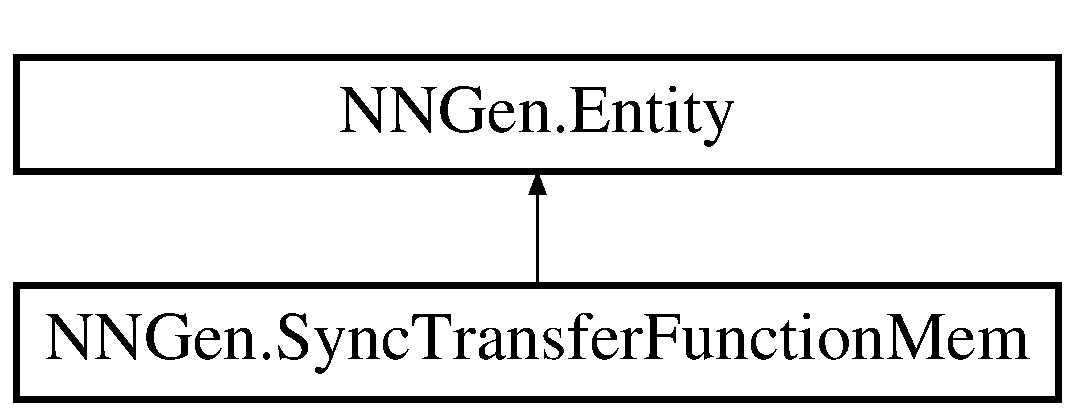
\includegraphics[height=2.000000cm]{class_n_n_gen_1_1_sync_transfer_function_mem}
\end{center}
\end{figure}
\subsection*{Public Member Functions}
\begin{DoxyCompactItemize}
\item 
\hyperlink{class_n_n_gen_1_1_sync_transfer_function_mem_ad19b1fb77caa8199d378760b7472f950}{Sync\+Transfer\+Function\+Mem} (int \+\_\+num\+Int\+Bits, int \+\_\+num\+Frac\+Bits, \hyperlink{class_n_n_gen_1_1_transfer_function_wrapper_aa338ffadb8fcdf76df75419374a51ff6}{Transfer\+Function\+Wrapper.\+Memory\+Activation\+Type} \+\_\+activation\+Type, string \+\_\+name)
\begin{DoxyCompactList}\small\item\em Create a new instance of a memory implementation of a synchronous transfer function \end{DoxyCompactList}\item 
override string \hyperlink{class_n_n_gen_1_1_sync_transfer_function_mem_ad4e64419e06ee98cd0a8e52d7ed866b6}{get\+Name} ()
\begin{DoxyCompactList}\small\item\em Returns the name of the entity \end{DoxyCompactList}\item 
override \hyperlink{class_n_n_gen_1_1_port}{Port}\mbox{[}$\,$\mbox{]} \hyperlink{class_n_n_gen_1_1_sync_transfer_function_mem_a4e263ba9743751277b49cd90578e2455}{get\+Input\+Ports} ()
\begin{DoxyCompactList}\small\item\em Returns the inputs to the device \end{DoxyCompactList}\item 
override \hyperlink{class_n_n_gen_1_1_port}{Port}\mbox{[}$\,$\mbox{]} \hyperlink{class_n_n_gen_1_1_sync_transfer_function_mem_a56548ab0fbafaa0384aa3c5cddc4d050}{get\+Output\+Ports} ()
\begin{DoxyCompactList}\small\item\em Returns the outputs to the device \end{DoxyCompactList}\item 
override \hyperlink{class_n_n_gen_1_1_signal}{Signal}\mbox{[}$\,$\mbox{]} \hyperlink{class_n_n_gen_1_1_sync_transfer_function_mem_a6b11efb6fd2d874b9bb5cfaafdb528a5}{get\+Internal\+Signals} ()
\begin{DoxyCompactList}\small\item\em Returns the internal signals for the device \end{DoxyCompactList}\item 
override bool \hyperlink{class_n_n_gen_1_1_sync_transfer_function_mem_a6262571443276194d157c94be915f069}{write\+V\+H\+D\+L} (string file)
\begin{DoxyCompactList}\small\item\em Writes the .vhd files necessary to compile this entity. All other necessary entities (i.\+e. neurons, thresholding functions, etc.) will also be written when this function returns \end{DoxyCompactList}\end{DoxyCompactItemize}
\subsection*{Public Attributes}
\begin{DoxyCompactItemize}
\item 
\hyperlink{class_n_n_gen_1_1_transfer_function_wrapper_aa338ffadb8fcdf76df75419374a51ff6}{Transfer\+Function\+Wrapper.\+Memory\+Activation\+Type} \hyperlink{class_n_n_gen_1_1_sync_transfer_function_mem_a98b2591ff8d7243cfc7546a7c37032d7}{activation\+Type}
\begin{DoxyCompactList}\small\item\em The transfer function to implement \end{DoxyCompactList}\end{DoxyCompactItemize}
\subsection*{Properties}
\begin{DoxyCompactItemize}
\item 
\hyperlink{class_n_n_gen_1_1_port}{Port} \hyperlink{class_n_n_gen_1_1_sync_transfer_function_mem_a842f5ef77e0b13f7e5a91b69fb10880b}{addr}\hspace{0.3cm}{\ttfamily  \mbox{[}get\mbox{]}}
\begin{DoxyCompactList}\small\item\em The address from which to read the memory \end{DoxyCompactList}\item 
\hyperlink{class_n_n_gen_1_1_port}{Port} \hyperlink{class_n_n_gen_1_1_sync_transfer_function_mem_a39eac2d524a3ed0d3e55762373f3879c}{clk}\hspace{0.3cm}{\ttfamily  \mbox{[}get\mbox{]}}
\begin{DoxyCompactList}\small\item\em The clock signal for the memory \end{DoxyCompactList}\item 
\hyperlink{class_n_n_gen_1_1_port}{Port} \hyperlink{class_n_n_gen_1_1_sync_transfer_function_mem_a1afdcfbaa9233adc7673c2a59724accb}{data}\hspace{0.3cm}{\ttfamily  \mbox{[}get\mbox{]}}
\begin{DoxyCompactList}\small\item\em The output of the memory \end{DoxyCompactList}\item 
int \hyperlink{class_n_n_gen_1_1_sync_transfer_function_mem_ac004657938e8276bfcaf430399237501}{num\+Int\+Bits}\hspace{0.3cm}{\ttfamily  \mbox{[}get\mbox{]}}
\begin{DoxyCompactList}\small\item\em The number of integer bits to use for the memory \end{DoxyCompactList}\item 
int \hyperlink{class_n_n_gen_1_1_sync_transfer_function_mem_ae036daf729a3381857761582bb573498}{num\+Frac\+Bits}\hspace{0.3cm}{\ttfamily  \mbox{[}get\mbox{]}}
\begin{DoxyCompactList}\small\item\em The number of fractional bits to use for the memory \end{DoxyCompactList}\item 
string \hyperlink{class_n_n_gen_1_1_sync_transfer_function_mem_adb5f86e770954ca55c554848ea65a5f8}{name}\hspace{0.3cm}{\ttfamily  \mbox{[}get\mbox{]}}
\begin{DoxyCompactList}\small\item\em The name of the memory instance \end{DoxyCompactList}\end{DoxyCompactItemize}


\subsection{Detailed Description}
A synchronous transfer function stored in memory. The transfer function is assumed to be symmetric around x = 0 



\subsection{Constructor \& Destructor Documentation}
\hypertarget{class_n_n_gen_1_1_sync_transfer_function_mem_ad19b1fb77caa8199d378760b7472f950}{}\index{N\+N\+Gen\+::\+Sync\+Transfer\+Function\+Mem@{N\+N\+Gen\+::\+Sync\+Transfer\+Function\+Mem}!Sync\+Transfer\+Function\+Mem@{Sync\+Transfer\+Function\+Mem}}
\index{Sync\+Transfer\+Function\+Mem@{Sync\+Transfer\+Function\+Mem}!N\+N\+Gen\+::\+Sync\+Transfer\+Function\+Mem@{N\+N\+Gen\+::\+Sync\+Transfer\+Function\+Mem}}
\subsubsection[{Sync\+Transfer\+Function\+Mem(int \+\_\+num\+Int\+Bits, int \+\_\+num\+Frac\+Bits, Transfer\+Function\+Wrapper.\+Memory\+Activation\+Type \+\_\+activation\+Type, string \+\_\+name)}]{\setlength{\rightskip}{0pt plus 5cm}N\+N\+Gen.\+Sync\+Transfer\+Function\+Mem.\+Sync\+Transfer\+Function\+Mem (
\begin{DoxyParamCaption}
\item[{int}]{\+\_\+num\+Int\+Bits, }
\item[{int}]{\+\_\+num\+Frac\+Bits, }
\item[{{\bf Transfer\+Function\+Wrapper.\+Memory\+Activation\+Type}}]{\+\_\+activation\+Type, }
\item[{string}]{\+\_\+name}
\end{DoxyParamCaption}
)\hspace{0.3cm}{\ttfamily [inline]}}\label{class_n_n_gen_1_1_sync_transfer_function_mem_ad19b1fb77caa8199d378760b7472f950}


Create a new instance of a memory implementation of a synchronous transfer function 


\begin{DoxyParams}{Parameters}
{\em \+\_\+num\+Int\+Bits} & The number of integer bits to use in the implementation\\
\hline
{\em \+\_\+num\+Frac\+Bits} & The number of fractional bits to use in the implementation\\
\hline
{\em \+\_\+activation\+Type} & The transfer function to implement\\
\hline
{\em \+\_\+name} & The name of the memory entity\\
\hline
\end{DoxyParams}


\subsection{Member Function Documentation}
\hypertarget{class_n_n_gen_1_1_sync_transfer_function_mem_a4e263ba9743751277b49cd90578e2455}{}\index{N\+N\+Gen\+::\+Sync\+Transfer\+Function\+Mem@{N\+N\+Gen\+::\+Sync\+Transfer\+Function\+Mem}!get\+Input\+Ports@{get\+Input\+Ports}}
\index{get\+Input\+Ports@{get\+Input\+Ports}!N\+N\+Gen\+::\+Sync\+Transfer\+Function\+Mem@{N\+N\+Gen\+::\+Sync\+Transfer\+Function\+Mem}}
\subsubsection[{get\+Input\+Ports()}]{\setlength{\rightskip}{0pt plus 5cm}override {\bf Port} \mbox{[}$\,$\mbox{]} N\+N\+Gen.\+Sync\+Transfer\+Function\+Mem.\+get\+Input\+Ports (
\begin{DoxyParamCaption}
{}
\end{DoxyParamCaption}
)\hspace{0.3cm}{\ttfamily [inline]}, {\ttfamily [virtual]}}\label{class_n_n_gen_1_1_sync_transfer_function_mem_a4e263ba9743751277b49cd90578e2455}


Returns the inputs to the device 

\begin{DoxyReturn}{Returns}
The inputs to the device
\end{DoxyReturn}


Implements \hyperlink{class_n_n_gen_1_1_entity_a01239f05c9efa61ec9e6a29cb2eaad50}{N\+N\+Gen.\+Entity}.

\hypertarget{class_n_n_gen_1_1_sync_transfer_function_mem_a6b11efb6fd2d874b9bb5cfaafdb528a5}{}\index{N\+N\+Gen\+::\+Sync\+Transfer\+Function\+Mem@{N\+N\+Gen\+::\+Sync\+Transfer\+Function\+Mem}!get\+Internal\+Signals@{get\+Internal\+Signals}}
\index{get\+Internal\+Signals@{get\+Internal\+Signals}!N\+N\+Gen\+::\+Sync\+Transfer\+Function\+Mem@{N\+N\+Gen\+::\+Sync\+Transfer\+Function\+Mem}}
\subsubsection[{get\+Internal\+Signals()}]{\setlength{\rightskip}{0pt plus 5cm}override {\bf Signal} \mbox{[}$\,$\mbox{]} N\+N\+Gen.\+Sync\+Transfer\+Function\+Mem.\+get\+Internal\+Signals (
\begin{DoxyParamCaption}
{}
\end{DoxyParamCaption}
)\hspace{0.3cm}{\ttfamily [inline]}, {\ttfamily [virtual]}}\label{class_n_n_gen_1_1_sync_transfer_function_mem_a6b11efb6fd2d874b9bb5cfaafdb528a5}


Returns the internal signals for the device 

\begin{DoxyReturn}{Returns}
The internal signals for the device
\end{DoxyReturn}


Implements \hyperlink{class_n_n_gen_1_1_entity_a62feb80e95ec84c650ea17bd53f0d510}{N\+N\+Gen.\+Entity}.

\hypertarget{class_n_n_gen_1_1_sync_transfer_function_mem_ad4e64419e06ee98cd0a8e52d7ed866b6}{}\index{N\+N\+Gen\+::\+Sync\+Transfer\+Function\+Mem@{N\+N\+Gen\+::\+Sync\+Transfer\+Function\+Mem}!get\+Name@{get\+Name}}
\index{get\+Name@{get\+Name}!N\+N\+Gen\+::\+Sync\+Transfer\+Function\+Mem@{N\+N\+Gen\+::\+Sync\+Transfer\+Function\+Mem}}
\subsubsection[{get\+Name()}]{\setlength{\rightskip}{0pt plus 5cm}override string N\+N\+Gen.\+Sync\+Transfer\+Function\+Mem.\+get\+Name (
\begin{DoxyParamCaption}
{}
\end{DoxyParamCaption}
)\hspace{0.3cm}{\ttfamily [inline]}, {\ttfamily [virtual]}}\label{class_n_n_gen_1_1_sync_transfer_function_mem_ad4e64419e06ee98cd0a8e52d7ed866b6}


Returns the name of the entity 

\begin{DoxyReturn}{Returns}
The name of the entity
\end{DoxyReturn}


Implements \hyperlink{class_n_n_gen_1_1_entity_a9f25d1070c9ab8ad343c28443e62e6f2}{N\+N\+Gen.\+Entity}.

\hypertarget{class_n_n_gen_1_1_sync_transfer_function_mem_a56548ab0fbafaa0384aa3c5cddc4d050}{}\index{N\+N\+Gen\+::\+Sync\+Transfer\+Function\+Mem@{N\+N\+Gen\+::\+Sync\+Transfer\+Function\+Mem}!get\+Output\+Ports@{get\+Output\+Ports}}
\index{get\+Output\+Ports@{get\+Output\+Ports}!N\+N\+Gen\+::\+Sync\+Transfer\+Function\+Mem@{N\+N\+Gen\+::\+Sync\+Transfer\+Function\+Mem}}
\subsubsection[{get\+Output\+Ports()}]{\setlength{\rightskip}{0pt plus 5cm}override {\bf Port} \mbox{[}$\,$\mbox{]} N\+N\+Gen.\+Sync\+Transfer\+Function\+Mem.\+get\+Output\+Ports (
\begin{DoxyParamCaption}
{}
\end{DoxyParamCaption}
)\hspace{0.3cm}{\ttfamily [inline]}, {\ttfamily [virtual]}}\label{class_n_n_gen_1_1_sync_transfer_function_mem_a56548ab0fbafaa0384aa3c5cddc4d050}


Returns the outputs to the device 

\begin{DoxyReturn}{Returns}
The outputs to the device
\end{DoxyReturn}


Implements \hyperlink{class_n_n_gen_1_1_entity_ace06368087778e254a5048c7d28747be}{N\+N\+Gen.\+Entity}.

\hypertarget{class_n_n_gen_1_1_sync_transfer_function_mem_a6262571443276194d157c94be915f069}{}\index{N\+N\+Gen\+::\+Sync\+Transfer\+Function\+Mem@{N\+N\+Gen\+::\+Sync\+Transfer\+Function\+Mem}!write\+V\+H\+D\+L@{write\+V\+H\+D\+L}}
\index{write\+V\+H\+D\+L@{write\+V\+H\+D\+L}!N\+N\+Gen\+::\+Sync\+Transfer\+Function\+Mem@{N\+N\+Gen\+::\+Sync\+Transfer\+Function\+Mem}}
\subsubsection[{write\+V\+H\+D\+L(string file)}]{\setlength{\rightskip}{0pt plus 5cm}override bool N\+N\+Gen.\+Sync\+Transfer\+Function\+Mem.\+write\+V\+H\+D\+L (
\begin{DoxyParamCaption}
\item[{string}]{file}
\end{DoxyParamCaption}
)\hspace{0.3cm}{\ttfamily [inline]}, {\ttfamily [virtual]}}\label{class_n_n_gen_1_1_sync_transfer_function_mem_a6262571443276194d157c94be915f069}


Writes the .vhd files necessary to compile this entity. All other necessary entities (i.\+e. neurons, thresholding functions, etc.) will also be written when this function returns 


\begin{DoxyParams}{Parameters}
{\em file} & The file path in which to write the files (do N\+O\+T include \char`\"{}...\+name.\+vhd\char`\"{}\\
\hline
\end{DoxyParams}
\begin{DoxyReturn}{Returns}
true if the files were written successfully, false otherwise
\end{DoxyReturn}


Implements \hyperlink{class_n_n_gen_1_1_entity_a1111d498446be08b20583b9625893a52}{N\+N\+Gen.\+Entity}.



\subsection{Member Data Documentation}
\hypertarget{class_n_n_gen_1_1_sync_transfer_function_mem_a98b2591ff8d7243cfc7546a7c37032d7}{}\index{N\+N\+Gen\+::\+Sync\+Transfer\+Function\+Mem@{N\+N\+Gen\+::\+Sync\+Transfer\+Function\+Mem}!activation\+Type@{activation\+Type}}
\index{activation\+Type@{activation\+Type}!N\+N\+Gen\+::\+Sync\+Transfer\+Function\+Mem@{N\+N\+Gen\+::\+Sync\+Transfer\+Function\+Mem}}
\subsubsection[{activation\+Type}]{\setlength{\rightskip}{0pt plus 5cm}{\bf Transfer\+Function\+Wrapper.\+Memory\+Activation\+Type} N\+N\+Gen.\+Sync\+Transfer\+Function\+Mem.\+activation\+Type}\label{class_n_n_gen_1_1_sync_transfer_function_mem_a98b2591ff8d7243cfc7546a7c37032d7}


The transfer function to implement 



\subsection{Property Documentation}
\hypertarget{class_n_n_gen_1_1_sync_transfer_function_mem_a842f5ef77e0b13f7e5a91b69fb10880b}{}\index{N\+N\+Gen\+::\+Sync\+Transfer\+Function\+Mem@{N\+N\+Gen\+::\+Sync\+Transfer\+Function\+Mem}!addr@{addr}}
\index{addr@{addr}!N\+N\+Gen\+::\+Sync\+Transfer\+Function\+Mem@{N\+N\+Gen\+::\+Sync\+Transfer\+Function\+Mem}}
\subsubsection[{addr}]{\setlength{\rightskip}{0pt plus 5cm}{\bf Port} N\+N\+Gen.\+Sync\+Transfer\+Function\+Mem.\+addr\hspace{0.3cm}{\ttfamily [get]}}\label{class_n_n_gen_1_1_sync_transfer_function_mem_a842f5ef77e0b13f7e5a91b69fb10880b}


The address from which to read the memory 

\hypertarget{class_n_n_gen_1_1_sync_transfer_function_mem_a39eac2d524a3ed0d3e55762373f3879c}{}\index{N\+N\+Gen\+::\+Sync\+Transfer\+Function\+Mem@{N\+N\+Gen\+::\+Sync\+Transfer\+Function\+Mem}!clk@{clk}}
\index{clk@{clk}!N\+N\+Gen\+::\+Sync\+Transfer\+Function\+Mem@{N\+N\+Gen\+::\+Sync\+Transfer\+Function\+Mem}}
\subsubsection[{clk}]{\setlength{\rightskip}{0pt plus 5cm}{\bf Port} N\+N\+Gen.\+Sync\+Transfer\+Function\+Mem.\+clk\hspace{0.3cm}{\ttfamily [get]}}\label{class_n_n_gen_1_1_sync_transfer_function_mem_a39eac2d524a3ed0d3e55762373f3879c}


The clock signal for the memory 

\hypertarget{class_n_n_gen_1_1_sync_transfer_function_mem_a1afdcfbaa9233adc7673c2a59724accb}{}\index{N\+N\+Gen\+::\+Sync\+Transfer\+Function\+Mem@{N\+N\+Gen\+::\+Sync\+Transfer\+Function\+Mem}!data@{data}}
\index{data@{data}!N\+N\+Gen\+::\+Sync\+Transfer\+Function\+Mem@{N\+N\+Gen\+::\+Sync\+Transfer\+Function\+Mem}}
\subsubsection[{data}]{\setlength{\rightskip}{0pt plus 5cm}{\bf Port} N\+N\+Gen.\+Sync\+Transfer\+Function\+Mem.\+data\hspace{0.3cm}{\ttfamily [get]}}\label{class_n_n_gen_1_1_sync_transfer_function_mem_a1afdcfbaa9233adc7673c2a59724accb}


The output of the memory 

\hypertarget{class_n_n_gen_1_1_sync_transfer_function_mem_adb5f86e770954ca55c554848ea65a5f8}{}\index{N\+N\+Gen\+::\+Sync\+Transfer\+Function\+Mem@{N\+N\+Gen\+::\+Sync\+Transfer\+Function\+Mem}!name@{name}}
\index{name@{name}!N\+N\+Gen\+::\+Sync\+Transfer\+Function\+Mem@{N\+N\+Gen\+::\+Sync\+Transfer\+Function\+Mem}}
\subsubsection[{name}]{\setlength{\rightskip}{0pt plus 5cm}string N\+N\+Gen.\+Sync\+Transfer\+Function\+Mem.\+name\hspace{0.3cm}{\ttfamily [get]}}\label{class_n_n_gen_1_1_sync_transfer_function_mem_adb5f86e770954ca55c554848ea65a5f8}


The name of the memory instance 

\hypertarget{class_n_n_gen_1_1_sync_transfer_function_mem_ae036daf729a3381857761582bb573498}{}\index{N\+N\+Gen\+::\+Sync\+Transfer\+Function\+Mem@{N\+N\+Gen\+::\+Sync\+Transfer\+Function\+Mem}!num\+Frac\+Bits@{num\+Frac\+Bits}}
\index{num\+Frac\+Bits@{num\+Frac\+Bits}!N\+N\+Gen\+::\+Sync\+Transfer\+Function\+Mem@{N\+N\+Gen\+::\+Sync\+Transfer\+Function\+Mem}}
\subsubsection[{num\+Frac\+Bits}]{\setlength{\rightskip}{0pt plus 5cm}int N\+N\+Gen.\+Sync\+Transfer\+Function\+Mem.\+num\+Frac\+Bits\hspace{0.3cm}{\ttfamily [get]}}\label{class_n_n_gen_1_1_sync_transfer_function_mem_ae036daf729a3381857761582bb573498}


The number of fractional bits to use for the memory 

\hypertarget{class_n_n_gen_1_1_sync_transfer_function_mem_ac004657938e8276bfcaf430399237501}{}\index{N\+N\+Gen\+::\+Sync\+Transfer\+Function\+Mem@{N\+N\+Gen\+::\+Sync\+Transfer\+Function\+Mem}!num\+Int\+Bits@{num\+Int\+Bits}}
\index{num\+Int\+Bits@{num\+Int\+Bits}!N\+N\+Gen\+::\+Sync\+Transfer\+Function\+Mem@{N\+N\+Gen\+::\+Sync\+Transfer\+Function\+Mem}}
\subsubsection[{num\+Int\+Bits}]{\setlength{\rightskip}{0pt plus 5cm}int N\+N\+Gen.\+Sync\+Transfer\+Function\+Mem.\+num\+Int\+Bits\hspace{0.3cm}{\ttfamily [get]}}\label{class_n_n_gen_1_1_sync_transfer_function_mem_ac004657938e8276bfcaf430399237501}


The number of integer bits to use for the memory 



The documentation for this class was generated from the following file\+:\begin{DoxyCompactItemize}
\item 
E\+:/\+Documents/\+Visual Studio 2013/\+Projects/\+Neural\+Network/\+N\+N\+Gen/\hyperlink{_sync_transfer_function_mem_8cs}{Sync\+Transfer\+Function\+Mem.\+cs}\end{DoxyCompactItemize}

\hypertarget{class_n_n_gen_1_1_thank_you}{}\section{N\+N\+Gen.\+Thank\+You Class Reference}
\label{class_n_n_gen_1_1_thank_you}\index{N\+N\+Gen.\+Thank\+You@{N\+N\+Gen.\+Thank\+You}}


Thanks the user for using the tool \+:)  


Inheritance diagram for N\+N\+Gen.\+Thank\+You\+:\begin{figure}[H]
\begin{center}
\leavevmode
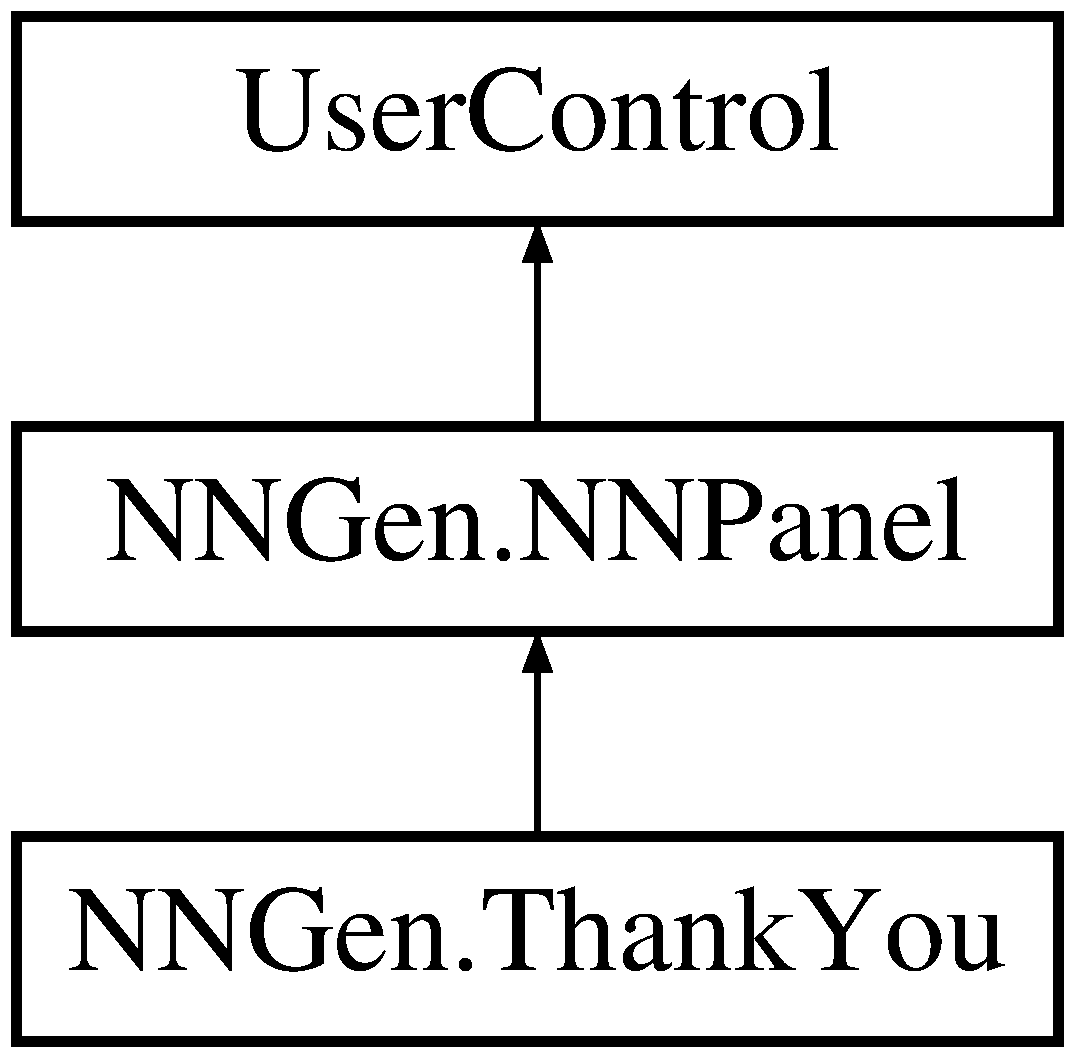
\includegraphics[height=3.000000cm]{class_n_n_gen_1_1_thank_you}
\end{center}
\end{figure}
\subsection*{Public Member Functions}
\begin{DoxyCompactItemize}
\item 
\hyperlink{class_n_n_gen_1_1_thank_you_a9b523a901e4d1d292cd7b47c18522b45}{Thank\+You} ()
\begin{DoxyCompactList}\small\item\em Initialize the form \end{DoxyCompactList}\end{DoxyCompactItemize}
\subsection*{Protected Member Functions}
\begin{DoxyCompactItemize}
\item 
override void \hyperlink{class_n_n_gen_1_1_thank_you_aa7cea980c28cc33b6df11e987cd3a3e3}{Dispose} (bool disposing)
\begin{DoxyCompactList}\small\item\em Clean up any resources being used. \end{DoxyCompactList}\end{DoxyCompactItemize}


\subsection{Detailed Description}
Thanks the user for using the tool \+:) 



\subsection{Constructor \& Destructor Documentation}
\hypertarget{class_n_n_gen_1_1_thank_you_a9b523a901e4d1d292cd7b47c18522b45}{}\index{N\+N\+Gen\+::\+Thank\+You@{N\+N\+Gen\+::\+Thank\+You}!Thank\+You@{Thank\+You}}
\index{Thank\+You@{Thank\+You}!N\+N\+Gen\+::\+Thank\+You@{N\+N\+Gen\+::\+Thank\+You}}
\subsubsection[{Thank\+You()}]{\setlength{\rightskip}{0pt plus 5cm}N\+N\+Gen.\+Thank\+You.\+Thank\+You (
\begin{DoxyParamCaption}
{}
\end{DoxyParamCaption}
)\hspace{0.3cm}{\ttfamily [inline]}}\label{class_n_n_gen_1_1_thank_you_a9b523a901e4d1d292cd7b47c18522b45}


Initialize the form 



\subsection{Member Function Documentation}
\hypertarget{class_n_n_gen_1_1_thank_you_aa7cea980c28cc33b6df11e987cd3a3e3}{}\index{N\+N\+Gen\+::\+Thank\+You@{N\+N\+Gen\+::\+Thank\+You}!Dispose@{Dispose}}
\index{Dispose@{Dispose}!N\+N\+Gen\+::\+Thank\+You@{N\+N\+Gen\+::\+Thank\+You}}
\subsubsection[{Dispose(bool disposing)}]{\setlength{\rightskip}{0pt plus 5cm}override void N\+N\+Gen.\+Thank\+You.\+Dispose (
\begin{DoxyParamCaption}
\item[{bool}]{disposing}
\end{DoxyParamCaption}
)\hspace{0.3cm}{\ttfamily [inline]}, {\ttfamily [protected]}}\label{class_n_n_gen_1_1_thank_you_aa7cea980c28cc33b6df11e987cd3a3e3}


Clean up any resources being used. 


\begin{DoxyParams}{Parameters}
{\em disposing} & true if managed resources should be disposed; otherwise, false.\\
\hline
\end{DoxyParams}


The documentation for this class was generated from the following files\+:\begin{DoxyCompactItemize}
\item 
E\+:/\+Documents/\+Visual Studio 2013/\+Projects/\+Neural\+Network/\+N\+N\+Gen/\hyperlink{_thank_you_8cs}{Thank\+You.\+cs}\item 
E\+:/\+Documents/\+Visual Studio 2013/\+Projects/\+Neural\+Network/\+N\+N\+Gen/\hyperlink{_thank_you_8_designer_8cs}{Thank\+You.\+Designer.\+cs}\end{DoxyCompactItemize}

\hypertarget{class_n_n_gen_1_1_transfer_function_wrapper}{}\section{N\+N\+Gen.\+Transfer\+Function\+Wrapper Class Reference}
\label{class_n_n_gen_1_1_transfer_function_wrapper}\index{N\+N\+Gen.\+Transfer\+Function\+Wrapper@{N\+N\+Gen.\+Transfer\+Function\+Wrapper}}


Initializes a wrapper for the transfer function memory element. As all implemented functions are symmetric around x = 0, we can save memory by only saving the values for x greater than 0 value in memory, and computing the x less than 0 values by (value = 1.\+0 -\/ abs(x)) Also, the functions implemented (aside from the Linear node) are very close to 1 or -\/1 when abs(x) $>$= 6.\+0, so when the input is in that range, the output is computed as\+: (out = 1.\+0 $\ast$ sgn(x)) (sgn = \{1 if x $>$ 0, -\/1 otherwise\}) (note, for Unipolar Sigmoid, the lower limit is 0, not -\/1)  


Inheritance diagram for N\+N\+Gen.\+Transfer\+Function\+Wrapper\+:\begin{figure}[H]
\begin{center}
\leavevmode
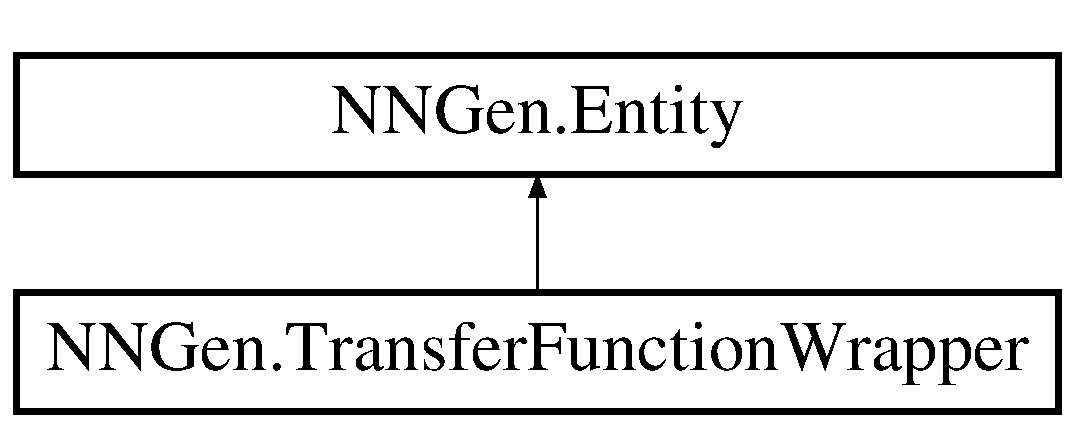
\includegraphics[height=2.000000cm]{class_n_n_gen_1_1_transfer_function_wrapper}
\end{center}
\end{figure}
\subsection*{Public Types}
\begin{DoxyCompactItemize}
\item 
enum \hyperlink{class_n_n_gen_1_1_transfer_function_wrapper_aa338ffadb8fcdf76df75419374a51ff6}{Memory\+Activation\+Type} \{ \hyperlink{class_n_n_gen_1_1_transfer_function_wrapper_aa338ffadb8fcdf76df75419374a51ff6aaac544aacc3615aada24897a215f5046}{Memory\+Activation\+Type.\+L\+I\+N\+E\+A\+R}, 
\hyperlink{class_n_n_gen_1_1_transfer_function_wrapper_aa338ffadb8fcdf76df75419374a51ff6a40a595040be78efa1c583f123663f8a8}{Memory\+Activation\+Type.\+U\+N\+I\+P\+O\+L\+A\+R\+\_\+\+S\+I\+G\+M\+O\+I\+D}, 
\hyperlink{class_n_n_gen_1_1_transfer_function_wrapper_aa338ffadb8fcdf76df75419374a51ff6ad465b2bacf5410a807fab76338ad95bd}{Memory\+Activation\+Type.\+B\+I\+P\+O\+L\+A\+R\+\_\+\+S\+I\+G\+M\+O\+I\+D}, 
\hyperlink{class_n_n_gen_1_1_transfer_function_wrapper_aa338ffadb8fcdf76df75419374a51ff6a1b8b4b9feedd482b4faaaa5ba9851770}{Memory\+Activation\+Type.\+H\+Y\+P\+E\+R\+B\+O\+L\+I\+C\+\_\+\+T\+A\+N\+G\+E\+N\+T}
 \}\begin{DoxyCompactList}\small\item\em The supported memory activation types \end{DoxyCompactList}
\end{DoxyCompactItemize}
\subsection*{Public Member Functions}
\begin{DoxyCompactItemize}
\item 
\hyperlink{class_n_n_gen_1_1_transfer_function_wrapper_a0d552d42c2b0d881b049d05c2fe7e3a9}{Transfer\+Function\+Wrapper} (int \+\_\+num\+Int\+Bits, int \+\_\+num\+Frac\+Bits, \hyperlink{class_n_n_gen_1_1_transfer_function_wrapper_aa338ffadb8fcdf76df75419374a51ff6}{Memory\+Activation\+Type} \+\_\+activation\+Type)
\begin{DoxyCompactList}\small\item\em Create a \hyperlink{class_n_n_gen_1_1_transfer_function_wrapper}{Transfer\+Function\+Wrapper} entity \end{DoxyCompactList}\item 
override string \hyperlink{class_n_n_gen_1_1_transfer_function_wrapper_a0ee97f1271edd325188fe389f1b25372}{get\+Name} ()
\begin{DoxyCompactList}\small\item\em Returns the name of the entity \end{DoxyCompactList}\item 
override \hyperlink{class_n_n_gen_1_1_port}{Port}\mbox{[}$\,$\mbox{]} \hyperlink{class_n_n_gen_1_1_transfer_function_wrapper_a383f86ef468440ca41a5018c8670c2ef}{get\+Input\+Ports} ()
\begin{DoxyCompactList}\small\item\em Returns the inputs to the device \end{DoxyCompactList}\item 
override \hyperlink{class_n_n_gen_1_1_port}{Port}\mbox{[}$\,$\mbox{]} \hyperlink{class_n_n_gen_1_1_transfer_function_wrapper_ae687574b26429fd7853a53df4759ca90}{get\+Output\+Ports} ()
\begin{DoxyCompactList}\small\item\em Returns the outputs to the device \end{DoxyCompactList}\item 
override \hyperlink{class_n_n_gen_1_1_signal}{Signal}\mbox{[}$\,$\mbox{]} \hyperlink{class_n_n_gen_1_1_transfer_function_wrapper_ae64279d96fae0f113bf6cf0cfbadfdff}{get\+Internal\+Signals} ()
\begin{DoxyCompactList}\small\item\em Returns the internal signals for the device \end{DoxyCompactList}\item 
override bool \hyperlink{class_n_n_gen_1_1_transfer_function_wrapper_a1c011e274cd2df8fc643228d77619890}{write\+V\+H\+D\+L} (string file)
\begin{DoxyCompactList}\small\item\em Writes the .vhd files necessary to compile this entity. All other necessary entities (i.\+e. neurons, thresholding functions, etc.) will also be written when this function returns \end{DoxyCompactList}\end{DoxyCompactItemize}
\subsection*{Properties}
\begin{DoxyCompactItemize}
\item 
string \hyperlink{class_n_n_gen_1_1_transfer_function_wrapper_a06c250469e511bdca837875720dbf5e9}{name}\hspace{0.3cm}{\ttfamily  \mbox{[}get\mbox{]}}
\begin{DoxyCompactList}\small\item\em The name of the \hyperlink{class_n_n_gen_1_1_transfer_function_wrapper}{Transfer\+Function\+Wrapper} entity \end{DoxyCompactList}\item 
\hyperlink{class_n_n_gen_1_1_port}{Port} \hyperlink{class_n_n_gen_1_1_transfer_function_wrapper_a0b1bd686fd58589ecee085e57596d2e7}{addr}\hspace{0.3cm}{\ttfamily  \mbox{[}get\mbox{]}}
\begin{DoxyCompactList}\small\item\em The address requested from memory (i.\+e. the value of x) \end{DoxyCompactList}\item 
\hyperlink{class_n_n_gen_1_1_port}{Port} \hyperlink{class_n_n_gen_1_1_transfer_function_wrapper_a4db456cd0b50d330f6b221032d35cc81}{clk}\hspace{0.3cm}{\ttfamily  \mbox{[}get\mbox{]}}
\begin{DoxyCompactList}\small\item\em The clock signal for the memory \end{DoxyCompactList}\item 
\hyperlink{class_n_n_gen_1_1_port}{Port} \hyperlink{class_n_n_gen_1_1_transfer_function_wrapper_a8898d56d022ccf0311e4cf7ed3ec138a}{data}\hspace{0.3cm}{\ttfamily  \mbox{[}get\mbox{]}}
\begin{DoxyCompactList}\small\item\em The output from the wrapper \end{DoxyCompactList}\item 
\hyperlink{class_n_n_gen_1_1_signal}{Signal} \hyperlink{class_n_n_gen_1_1_transfer_function_wrapper_ac952bf20fb4cef97074cadcb2971b1bd}{inverse\+Addr\+Temp}\hspace{0.3cm}{\ttfamily  \mbox{[}get\mbox{]}}
\begin{DoxyCompactList}\small\item\em Used in computing the value (-\/1 $\ast$ Addr) \end{DoxyCompactList}\item 
\hyperlink{class_n_n_gen_1_1_signal}{Signal} \hyperlink{class_n_n_gen_1_1_transfer_function_wrapper_acb5029596b5ce5da76a4fff79d6a10b0}{inverse\+Addr}\hspace{0.3cm}{\ttfamily  \mbox{[}get\mbox{]}}
\begin{DoxyCompactList}\small\item\em Holds the value (-\/1 $\ast$ Addr) \end{DoxyCompactList}\item 
\hyperlink{class_n_n_gen_1_1_signal}{Signal} \hyperlink{class_n_n_gen_1_1_transfer_function_wrapper_a60c3f55dade25c86f36d0524bcaadf6e}{mem\+Addr}\hspace{0.3cm}{\ttfamily  \mbox{[}get\mbox{]}}
\begin{DoxyCompactList}\small\item\em The address from memory to grab \end{DoxyCompactList}\item 
\hyperlink{class_n_n_gen_1_1_signal}{Signal} \hyperlink{class_n_n_gen_1_1_transfer_function_wrapper_a164219eb34ccaf82e0ee47ad3dcd3c25}{mem\+Out}\hspace{0.3cm}{\ttfamily  \mbox{[}get\mbox{]}}
\begin{DoxyCompactList}\small\item\em The output of the memory \end{DoxyCompactList}\item 
\hyperlink{class_n_n_gen_1_1_signal}{Signal} \hyperlink{class_n_n_gen_1_1_transfer_function_wrapper_aec4c1de29fdd1ffae3ac087477973d48}{mem\+Out\+\_\+sfixed}\hspace{0.3cm}{\ttfamily  \mbox{[}get\mbox{]}}
\begin{DoxyCompactList}\small\item\em The output of the memory, cast to sfixed \end{DoxyCompactList}\item 
\hyperlink{class_n_n_gen_1_1_signal}{Signal} \hyperlink{class_n_n_gen_1_1_transfer_function_wrapper_a28102412789e840a8d62d4f1d80b6fce}{one\+Minus\+Mem\+Out\+\_\+sfixed}\hspace{0.3cm}{\ttfamily  \mbox{[}get\mbox{]}}
\begin{DoxyCompactList}\small\item\em Holds the value of 1 -\/ output (used to compute the values when the input is less than 0) \end{DoxyCompactList}\item 
\hyperlink{class_n_n_gen_1_1_signal}{Signal} \hyperlink{class_n_n_gen_1_1_transfer_function_wrapper_a5775b19c91e1a869c0c5e7587aaa4a00}{out\+Sig}\hspace{0.3cm}{\ttfamily  \mbox{[}get\mbox{]}}
\begin{DoxyCompactList}\small\item\em The output of the device \end{DoxyCompactList}\item 
\hyperlink{class_n_n_gen_1_1_transfer_function_wrapper_aa338ffadb8fcdf76df75419374a51ff6}{Memory\+Activation\+Type} \hyperlink{class_n_n_gen_1_1_transfer_function_wrapper_a6e15bcbf79f66a23f040cbcc69fec3d2}{activation\+Type}\hspace{0.3cm}{\ttfamily  \mbox{[}get\mbox{]}}
\begin{DoxyCompactList}\small\item\em The memory activation type to implement \end{DoxyCompactList}\item 
\hyperlink{class_n_n_gen_1_1_sync_transfer_function_mem}{Sync\+Transfer\+Function\+Mem} \hyperlink{class_n_n_gen_1_1_transfer_function_wrapper_aecb111b0e3e39a4dec337da6288341f4}{sm}\hspace{0.3cm}{\ttfamily  \mbox{[}get\mbox{]}}
\begin{DoxyCompactList}\small\item\em The memory entity from which to read the transfer function \end{DoxyCompactList}\end{DoxyCompactItemize}


\subsection{Detailed Description}
Initializes a wrapper for the transfer function memory element. As all implemented functions are symmetric around x = 0, we can save memory by only saving the values for x greater than 0 value in memory, and computing the x less than 0 values by (value = 1.\+0 -\/ abs(x)) Also, the functions implemented (aside from the Linear node) are very close to 1 or -\/1 when abs(x) $>$= 6.\+0, so when the input is in that range, the output is computed as\+: (out = 1.\+0 $\ast$ sgn(x)) (sgn = \{1 if x $>$ 0, -\/1 otherwise\}) (note, for Unipolar Sigmoid, the lower limit is 0, not -\/1) 



\subsection{Member Enumeration Documentation}
\hypertarget{class_n_n_gen_1_1_transfer_function_wrapper_aa338ffadb8fcdf76df75419374a51ff6}{}\index{N\+N\+Gen\+::\+Transfer\+Function\+Wrapper@{N\+N\+Gen\+::\+Transfer\+Function\+Wrapper}!Memory\+Activation\+Type@{Memory\+Activation\+Type}}
\index{Memory\+Activation\+Type@{Memory\+Activation\+Type}!N\+N\+Gen\+::\+Transfer\+Function\+Wrapper@{N\+N\+Gen\+::\+Transfer\+Function\+Wrapper}}
\subsubsection[{Memory\+Activation\+Type}]{\setlength{\rightskip}{0pt plus 5cm}enum {\bf N\+N\+Gen.\+Transfer\+Function\+Wrapper.\+Memory\+Activation\+Type}\hspace{0.3cm}{\ttfamily [strong]}}\label{class_n_n_gen_1_1_transfer_function_wrapper_aa338ffadb8fcdf76df75419374a51ff6}


The supported memory activation types 

\begin{Desc}
\item[Enumerator]\par
\begin{description}
\index{L\+I\+N\+E\+A\+R@{L\+I\+N\+E\+A\+R}!N\+N\+Gen\+::\+Transfer\+Function\+Wrapper@{N\+N\+Gen\+::\+Transfer\+Function\+Wrapper}}\index{N\+N\+Gen\+::\+Transfer\+Function\+Wrapper@{N\+N\+Gen\+::\+Transfer\+Function\+Wrapper}!L\+I\+N\+E\+A\+R@{L\+I\+N\+E\+A\+R}}\item[{\em 
\hypertarget{class_n_n_gen_1_1_transfer_function_wrapper_aa338ffadb8fcdf76df75419374a51ff6aaac544aacc3615aada24897a215f5046}{}L\+I\+N\+E\+A\+R\label{class_n_n_gen_1_1_transfer_function_wrapper_aa338ffadb8fcdf76df75419374a51ff6aaac544aacc3615aada24897a215f5046}
}]Linear\+: F(x) = x \index{U\+N\+I\+P\+O\+L\+A\+R\+\_\+\+S\+I\+G\+M\+O\+I\+D@{U\+N\+I\+P\+O\+L\+A\+R\+\_\+\+S\+I\+G\+M\+O\+I\+D}!N\+N\+Gen\+::\+Transfer\+Function\+Wrapper@{N\+N\+Gen\+::\+Transfer\+Function\+Wrapper}}\index{N\+N\+Gen\+::\+Transfer\+Function\+Wrapper@{N\+N\+Gen\+::\+Transfer\+Function\+Wrapper}!U\+N\+I\+P\+O\+L\+A\+R\+\_\+\+S\+I\+G\+M\+O\+I\+D@{U\+N\+I\+P\+O\+L\+A\+R\+\_\+\+S\+I\+G\+M\+O\+I\+D}}\item[{\em 
\hypertarget{class_n_n_gen_1_1_transfer_function_wrapper_aa338ffadb8fcdf76df75419374a51ff6a40a595040be78efa1c583f123663f8a8}{}U\+N\+I\+P\+O\+L\+A\+R\+\_\+\+S\+I\+G\+M\+O\+I\+D\label{class_n_n_gen_1_1_transfer_function_wrapper_aa338ffadb8fcdf76df75419374a51ff6a40a595040be78efa1c583f123663f8a8}
}]Unipolar sigmoid\+: F(x) = 1 / (1 + exp(-\/x)) \index{B\+I\+P\+O\+L\+A\+R\+\_\+\+S\+I\+G\+M\+O\+I\+D@{B\+I\+P\+O\+L\+A\+R\+\_\+\+S\+I\+G\+M\+O\+I\+D}!N\+N\+Gen\+::\+Transfer\+Function\+Wrapper@{N\+N\+Gen\+::\+Transfer\+Function\+Wrapper}}\index{N\+N\+Gen\+::\+Transfer\+Function\+Wrapper@{N\+N\+Gen\+::\+Transfer\+Function\+Wrapper}!B\+I\+P\+O\+L\+A\+R\+\_\+\+S\+I\+G\+M\+O\+I\+D@{B\+I\+P\+O\+L\+A\+R\+\_\+\+S\+I\+G\+M\+O\+I\+D}}\item[{\em 
\hypertarget{class_n_n_gen_1_1_transfer_function_wrapper_aa338ffadb8fcdf76df75419374a51ff6ad465b2bacf5410a807fab76338ad95bd}{}B\+I\+P\+O\+L\+A\+R\+\_\+\+S\+I\+G\+M\+O\+I\+D\label{class_n_n_gen_1_1_transfer_function_wrapper_aa338ffadb8fcdf76df75419374a51ff6ad465b2bacf5410a807fab76338ad95bd}
}]Bipolar sigmoid\+: F(x) = -\/1 + (2 / (1 + exp(-\/x)) \index{H\+Y\+P\+E\+R\+B\+O\+L\+I\+C\+\_\+\+T\+A\+N\+G\+E\+N\+T@{H\+Y\+P\+E\+R\+B\+O\+L\+I\+C\+\_\+\+T\+A\+N\+G\+E\+N\+T}!N\+N\+Gen\+::\+Transfer\+Function\+Wrapper@{N\+N\+Gen\+::\+Transfer\+Function\+Wrapper}}\index{N\+N\+Gen\+::\+Transfer\+Function\+Wrapper@{N\+N\+Gen\+::\+Transfer\+Function\+Wrapper}!H\+Y\+P\+E\+R\+B\+O\+L\+I\+C\+\_\+\+T\+A\+N\+G\+E\+N\+T@{H\+Y\+P\+E\+R\+B\+O\+L\+I\+C\+\_\+\+T\+A\+N\+G\+E\+N\+T}}\item[{\em 
\hypertarget{class_n_n_gen_1_1_transfer_function_wrapper_aa338ffadb8fcdf76df75419374a51ff6a1b8b4b9feedd482b4faaaa5ba9851770}{}H\+Y\+P\+E\+R\+B\+O\+L\+I\+C\+\_\+\+T\+A\+N\+G\+E\+N\+T\label{class_n_n_gen_1_1_transfer_function_wrapper_aa338ffadb8fcdf76df75419374a51ff6a1b8b4b9feedd482b4faaaa5ba9851770}
}]Hyperbolic Tangent\+: F(\+X) = tanh(x) \end{description}
\end{Desc}


\subsection{Constructor \& Destructor Documentation}
\hypertarget{class_n_n_gen_1_1_transfer_function_wrapper_a0d552d42c2b0d881b049d05c2fe7e3a9}{}\index{N\+N\+Gen\+::\+Transfer\+Function\+Wrapper@{N\+N\+Gen\+::\+Transfer\+Function\+Wrapper}!Transfer\+Function\+Wrapper@{Transfer\+Function\+Wrapper}}
\index{Transfer\+Function\+Wrapper@{Transfer\+Function\+Wrapper}!N\+N\+Gen\+::\+Transfer\+Function\+Wrapper@{N\+N\+Gen\+::\+Transfer\+Function\+Wrapper}}
\subsubsection[{Transfer\+Function\+Wrapper(int \+\_\+num\+Int\+Bits, int \+\_\+num\+Frac\+Bits, Memory\+Activation\+Type \+\_\+activation\+Type)}]{\setlength{\rightskip}{0pt plus 5cm}N\+N\+Gen.\+Transfer\+Function\+Wrapper.\+Transfer\+Function\+Wrapper (
\begin{DoxyParamCaption}
\item[{int}]{\+\_\+num\+Int\+Bits, }
\item[{int}]{\+\_\+num\+Frac\+Bits, }
\item[{{\bf Memory\+Activation\+Type}}]{\+\_\+activation\+Type}
\end{DoxyParamCaption}
)\hspace{0.3cm}{\ttfamily [inline]}}\label{class_n_n_gen_1_1_transfer_function_wrapper_a0d552d42c2b0d881b049d05c2fe7e3a9}


Create a \hyperlink{class_n_n_gen_1_1_transfer_function_wrapper}{Transfer\+Function\+Wrapper} entity 


\begin{DoxyParams}{Parameters}
{\em \+\_\+num\+Int\+Bits} & The number of integer bits to use\\
\hline
{\em \+\_\+num\+Frac\+Bits} & The number of fractional bits to use\\
\hline
{\em \+\_\+activation\+Type} & The activation type to implement\\
\hline
\end{DoxyParams}


\subsection{Member Function Documentation}
\hypertarget{class_n_n_gen_1_1_transfer_function_wrapper_a383f86ef468440ca41a5018c8670c2ef}{}\index{N\+N\+Gen\+::\+Transfer\+Function\+Wrapper@{N\+N\+Gen\+::\+Transfer\+Function\+Wrapper}!get\+Input\+Ports@{get\+Input\+Ports}}
\index{get\+Input\+Ports@{get\+Input\+Ports}!N\+N\+Gen\+::\+Transfer\+Function\+Wrapper@{N\+N\+Gen\+::\+Transfer\+Function\+Wrapper}}
\subsubsection[{get\+Input\+Ports()}]{\setlength{\rightskip}{0pt plus 5cm}override {\bf Port} \mbox{[}$\,$\mbox{]} N\+N\+Gen.\+Transfer\+Function\+Wrapper.\+get\+Input\+Ports (
\begin{DoxyParamCaption}
{}
\end{DoxyParamCaption}
)\hspace{0.3cm}{\ttfamily [inline]}, {\ttfamily [virtual]}}\label{class_n_n_gen_1_1_transfer_function_wrapper_a383f86ef468440ca41a5018c8670c2ef}


Returns the inputs to the device 

\begin{DoxyReturn}{Returns}
The inputs to the device
\end{DoxyReturn}


Implements \hyperlink{class_n_n_gen_1_1_entity_a01239f05c9efa61ec9e6a29cb2eaad50}{N\+N\+Gen.\+Entity}.

\hypertarget{class_n_n_gen_1_1_transfer_function_wrapper_ae64279d96fae0f113bf6cf0cfbadfdff}{}\index{N\+N\+Gen\+::\+Transfer\+Function\+Wrapper@{N\+N\+Gen\+::\+Transfer\+Function\+Wrapper}!get\+Internal\+Signals@{get\+Internal\+Signals}}
\index{get\+Internal\+Signals@{get\+Internal\+Signals}!N\+N\+Gen\+::\+Transfer\+Function\+Wrapper@{N\+N\+Gen\+::\+Transfer\+Function\+Wrapper}}
\subsubsection[{get\+Internal\+Signals()}]{\setlength{\rightskip}{0pt plus 5cm}override {\bf Signal} \mbox{[}$\,$\mbox{]} N\+N\+Gen.\+Transfer\+Function\+Wrapper.\+get\+Internal\+Signals (
\begin{DoxyParamCaption}
{}
\end{DoxyParamCaption}
)\hspace{0.3cm}{\ttfamily [inline]}, {\ttfamily [virtual]}}\label{class_n_n_gen_1_1_transfer_function_wrapper_ae64279d96fae0f113bf6cf0cfbadfdff}


Returns the internal signals for the device 

\begin{DoxyReturn}{Returns}
The internal signals for the device
\end{DoxyReturn}


Implements \hyperlink{class_n_n_gen_1_1_entity_a62feb80e95ec84c650ea17bd53f0d510}{N\+N\+Gen.\+Entity}.

\hypertarget{class_n_n_gen_1_1_transfer_function_wrapper_a0ee97f1271edd325188fe389f1b25372}{}\index{N\+N\+Gen\+::\+Transfer\+Function\+Wrapper@{N\+N\+Gen\+::\+Transfer\+Function\+Wrapper}!get\+Name@{get\+Name}}
\index{get\+Name@{get\+Name}!N\+N\+Gen\+::\+Transfer\+Function\+Wrapper@{N\+N\+Gen\+::\+Transfer\+Function\+Wrapper}}
\subsubsection[{get\+Name()}]{\setlength{\rightskip}{0pt plus 5cm}override string N\+N\+Gen.\+Transfer\+Function\+Wrapper.\+get\+Name (
\begin{DoxyParamCaption}
{}
\end{DoxyParamCaption}
)\hspace{0.3cm}{\ttfamily [inline]}, {\ttfamily [virtual]}}\label{class_n_n_gen_1_1_transfer_function_wrapper_a0ee97f1271edd325188fe389f1b25372}


Returns the name of the entity 

\begin{DoxyReturn}{Returns}
The name of the entity
\end{DoxyReturn}


Implements \hyperlink{class_n_n_gen_1_1_entity_a9f25d1070c9ab8ad343c28443e62e6f2}{N\+N\+Gen.\+Entity}.

\hypertarget{class_n_n_gen_1_1_transfer_function_wrapper_ae687574b26429fd7853a53df4759ca90}{}\index{N\+N\+Gen\+::\+Transfer\+Function\+Wrapper@{N\+N\+Gen\+::\+Transfer\+Function\+Wrapper}!get\+Output\+Ports@{get\+Output\+Ports}}
\index{get\+Output\+Ports@{get\+Output\+Ports}!N\+N\+Gen\+::\+Transfer\+Function\+Wrapper@{N\+N\+Gen\+::\+Transfer\+Function\+Wrapper}}
\subsubsection[{get\+Output\+Ports()}]{\setlength{\rightskip}{0pt plus 5cm}override {\bf Port} \mbox{[}$\,$\mbox{]} N\+N\+Gen.\+Transfer\+Function\+Wrapper.\+get\+Output\+Ports (
\begin{DoxyParamCaption}
{}
\end{DoxyParamCaption}
)\hspace{0.3cm}{\ttfamily [inline]}, {\ttfamily [virtual]}}\label{class_n_n_gen_1_1_transfer_function_wrapper_ae687574b26429fd7853a53df4759ca90}


Returns the outputs to the device 

\begin{DoxyReturn}{Returns}
The outputs to the device
\end{DoxyReturn}


Implements \hyperlink{class_n_n_gen_1_1_entity_ace06368087778e254a5048c7d28747be}{N\+N\+Gen.\+Entity}.

\hypertarget{class_n_n_gen_1_1_transfer_function_wrapper_a1c011e274cd2df8fc643228d77619890}{}\index{N\+N\+Gen\+::\+Transfer\+Function\+Wrapper@{N\+N\+Gen\+::\+Transfer\+Function\+Wrapper}!write\+V\+H\+D\+L@{write\+V\+H\+D\+L}}
\index{write\+V\+H\+D\+L@{write\+V\+H\+D\+L}!N\+N\+Gen\+::\+Transfer\+Function\+Wrapper@{N\+N\+Gen\+::\+Transfer\+Function\+Wrapper}}
\subsubsection[{write\+V\+H\+D\+L(string file)}]{\setlength{\rightskip}{0pt plus 5cm}override bool N\+N\+Gen.\+Transfer\+Function\+Wrapper.\+write\+V\+H\+D\+L (
\begin{DoxyParamCaption}
\item[{string}]{file}
\end{DoxyParamCaption}
)\hspace{0.3cm}{\ttfamily [inline]}, {\ttfamily [virtual]}}\label{class_n_n_gen_1_1_transfer_function_wrapper_a1c011e274cd2df8fc643228d77619890}


Writes the .vhd files necessary to compile this entity. All other necessary entities (i.\+e. neurons, thresholding functions, etc.) will also be written when this function returns 


\begin{DoxyParams}{Parameters}
{\em file} & The file path in which to write the files (do N\+O\+T include \char`\"{}...\+name.\+vhd\char`\"{}\\
\hline
\end{DoxyParams}
\begin{DoxyReturn}{Returns}
true if the files were written successfully, false otherwise
\end{DoxyReturn}


Implements \hyperlink{class_n_n_gen_1_1_entity_a1111d498446be08b20583b9625893a52}{N\+N\+Gen.\+Entity}.



\subsection{Property Documentation}
\hypertarget{class_n_n_gen_1_1_transfer_function_wrapper_a6e15bcbf79f66a23f040cbcc69fec3d2}{}\index{N\+N\+Gen\+::\+Transfer\+Function\+Wrapper@{N\+N\+Gen\+::\+Transfer\+Function\+Wrapper}!activation\+Type@{activation\+Type}}
\index{activation\+Type@{activation\+Type}!N\+N\+Gen\+::\+Transfer\+Function\+Wrapper@{N\+N\+Gen\+::\+Transfer\+Function\+Wrapper}}
\subsubsection[{activation\+Type}]{\setlength{\rightskip}{0pt plus 5cm}{\bf Memory\+Activation\+Type} N\+N\+Gen.\+Transfer\+Function\+Wrapper.\+activation\+Type\hspace{0.3cm}{\ttfamily [get]}}\label{class_n_n_gen_1_1_transfer_function_wrapper_a6e15bcbf79f66a23f040cbcc69fec3d2}


The memory activation type to implement 

\hypertarget{class_n_n_gen_1_1_transfer_function_wrapper_a0b1bd686fd58589ecee085e57596d2e7}{}\index{N\+N\+Gen\+::\+Transfer\+Function\+Wrapper@{N\+N\+Gen\+::\+Transfer\+Function\+Wrapper}!addr@{addr}}
\index{addr@{addr}!N\+N\+Gen\+::\+Transfer\+Function\+Wrapper@{N\+N\+Gen\+::\+Transfer\+Function\+Wrapper}}
\subsubsection[{addr}]{\setlength{\rightskip}{0pt plus 5cm}{\bf Port} N\+N\+Gen.\+Transfer\+Function\+Wrapper.\+addr\hspace{0.3cm}{\ttfamily [get]}}\label{class_n_n_gen_1_1_transfer_function_wrapper_a0b1bd686fd58589ecee085e57596d2e7}


The address requested from memory (i.\+e. the value of x) 

\hypertarget{class_n_n_gen_1_1_transfer_function_wrapper_a4db456cd0b50d330f6b221032d35cc81}{}\index{N\+N\+Gen\+::\+Transfer\+Function\+Wrapper@{N\+N\+Gen\+::\+Transfer\+Function\+Wrapper}!clk@{clk}}
\index{clk@{clk}!N\+N\+Gen\+::\+Transfer\+Function\+Wrapper@{N\+N\+Gen\+::\+Transfer\+Function\+Wrapper}}
\subsubsection[{clk}]{\setlength{\rightskip}{0pt plus 5cm}{\bf Port} N\+N\+Gen.\+Transfer\+Function\+Wrapper.\+clk\hspace{0.3cm}{\ttfamily [get]}}\label{class_n_n_gen_1_1_transfer_function_wrapper_a4db456cd0b50d330f6b221032d35cc81}


The clock signal for the memory 

\hypertarget{class_n_n_gen_1_1_transfer_function_wrapper_a8898d56d022ccf0311e4cf7ed3ec138a}{}\index{N\+N\+Gen\+::\+Transfer\+Function\+Wrapper@{N\+N\+Gen\+::\+Transfer\+Function\+Wrapper}!data@{data}}
\index{data@{data}!N\+N\+Gen\+::\+Transfer\+Function\+Wrapper@{N\+N\+Gen\+::\+Transfer\+Function\+Wrapper}}
\subsubsection[{data}]{\setlength{\rightskip}{0pt plus 5cm}{\bf Port} N\+N\+Gen.\+Transfer\+Function\+Wrapper.\+data\hspace{0.3cm}{\ttfamily [get]}}\label{class_n_n_gen_1_1_transfer_function_wrapper_a8898d56d022ccf0311e4cf7ed3ec138a}


The output from the wrapper 

\hypertarget{class_n_n_gen_1_1_transfer_function_wrapper_acb5029596b5ce5da76a4fff79d6a10b0}{}\index{N\+N\+Gen\+::\+Transfer\+Function\+Wrapper@{N\+N\+Gen\+::\+Transfer\+Function\+Wrapper}!inverse\+Addr@{inverse\+Addr}}
\index{inverse\+Addr@{inverse\+Addr}!N\+N\+Gen\+::\+Transfer\+Function\+Wrapper@{N\+N\+Gen\+::\+Transfer\+Function\+Wrapper}}
\subsubsection[{inverse\+Addr}]{\setlength{\rightskip}{0pt plus 5cm}{\bf Signal} N\+N\+Gen.\+Transfer\+Function\+Wrapper.\+inverse\+Addr\hspace{0.3cm}{\ttfamily [get]}}\label{class_n_n_gen_1_1_transfer_function_wrapper_acb5029596b5ce5da76a4fff79d6a10b0}


Holds the value (-\/1 $\ast$ Addr) 

\hypertarget{class_n_n_gen_1_1_transfer_function_wrapper_ac952bf20fb4cef97074cadcb2971b1bd}{}\index{N\+N\+Gen\+::\+Transfer\+Function\+Wrapper@{N\+N\+Gen\+::\+Transfer\+Function\+Wrapper}!inverse\+Addr\+Temp@{inverse\+Addr\+Temp}}
\index{inverse\+Addr\+Temp@{inverse\+Addr\+Temp}!N\+N\+Gen\+::\+Transfer\+Function\+Wrapper@{N\+N\+Gen\+::\+Transfer\+Function\+Wrapper}}
\subsubsection[{inverse\+Addr\+Temp}]{\setlength{\rightskip}{0pt plus 5cm}{\bf Signal} N\+N\+Gen.\+Transfer\+Function\+Wrapper.\+inverse\+Addr\+Temp\hspace{0.3cm}{\ttfamily [get]}}\label{class_n_n_gen_1_1_transfer_function_wrapper_ac952bf20fb4cef97074cadcb2971b1bd}


Used in computing the value (-\/1 $\ast$ Addr) 

\hypertarget{class_n_n_gen_1_1_transfer_function_wrapper_a60c3f55dade25c86f36d0524bcaadf6e}{}\index{N\+N\+Gen\+::\+Transfer\+Function\+Wrapper@{N\+N\+Gen\+::\+Transfer\+Function\+Wrapper}!mem\+Addr@{mem\+Addr}}
\index{mem\+Addr@{mem\+Addr}!N\+N\+Gen\+::\+Transfer\+Function\+Wrapper@{N\+N\+Gen\+::\+Transfer\+Function\+Wrapper}}
\subsubsection[{mem\+Addr}]{\setlength{\rightskip}{0pt plus 5cm}{\bf Signal} N\+N\+Gen.\+Transfer\+Function\+Wrapper.\+mem\+Addr\hspace{0.3cm}{\ttfamily [get]}}\label{class_n_n_gen_1_1_transfer_function_wrapper_a60c3f55dade25c86f36d0524bcaadf6e}


The address from memory to grab 

\hypertarget{class_n_n_gen_1_1_transfer_function_wrapper_a164219eb34ccaf82e0ee47ad3dcd3c25}{}\index{N\+N\+Gen\+::\+Transfer\+Function\+Wrapper@{N\+N\+Gen\+::\+Transfer\+Function\+Wrapper}!mem\+Out@{mem\+Out}}
\index{mem\+Out@{mem\+Out}!N\+N\+Gen\+::\+Transfer\+Function\+Wrapper@{N\+N\+Gen\+::\+Transfer\+Function\+Wrapper}}
\subsubsection[{mem\+Out}]{\setlength{\rightskip}{0pt plus 5cm}{\bf Signal} N\+N\+Gen.\+Transfer\+Function\+Wrapper.\+mem\+Out\hspace{0.3cm}{\ttfamily [get]}}\label{class_n_n_gen_1_1_transfer_function_wrapper_a164219eb34ccaf82e0ee47ad3dcd3c25}


The output of the memory 

\hypertarget{class_n_n_gen_1_1_transfer_function_wrapper_aec4c1de29fdd1ffae3ac087477973d48}{}\index{N\+N\+Gen\+::\+Transfer\+Function\+Wrapper@{N\+N\+Gen\+::\+Transfer\+Function\+Wrapper}!mem\+Out\+\_\+sfixed@{mem\+Out\+\_\+sfixed}}
\index{mem\+Out\+\_\+sfixed@{mem\+Out\+\_\+sfixed}!N\+N\+Gen\+::\+Transfer\+Function\+Wrapper@{N\+N\+Gen\+::\+Transfer\+Function\+Wrapper}}
\subsubsection[{mem\+Out\+\_\+sfixed}]{\setlength{\rightskip}{0pt plus 5cm}{\bf Signal} N\+N\+Gen.\+Transfer\+Function\+Wrapper.\+mem\+Out\+\_\+sfixed\hspace{0.3cm}{\ttfamily [get]}}\label{class_n_n_gen_1_1_transfer_function_wrapper_aec4c1de29fdd1ffae3ac087477973d48}


The output of the memory, cast to sfixed 

\hypertarget{class_n_n_gen_1_1_transfer_function_wrapper_a06c250469e511bdca837875720dbf5e9}{}\index{N\+N\+Gen\+::\+Transfer\+Function\+Wrapper@{N\+N\+Gen\+::\+Transfer\+Function\+Wrapper}!name@{name}}
\index{name@{name}!N\+N\+Gen\+::\+Transfer\+Function\+Wrapper@{N\+N\+Gen\+::\+Transfer\+Function\+Wrapper}}
\subsubsection[{name}]{\setlength{\rightskip}{0pt plus 5cm}string N\+N\+Gen.\+Transfer\+Function\+Wrapper.\+name\hspace{0.3cm}{\ttfamily [get]}}\label{class_n_n_gen_1_1_transfer_function_wrapper_a06c250469e511bdca837875720dbf5e9}


The name of the \hyperlink{class_n_n_gen_1_1_transfer_function_wrapper}{Transfer\+Function\+Wrapper} entity 

\hypertarget{class_n_n_gen_1_1_transfer_function_wrapper_a28102412789e840a8d62d4f1d80b6fce}{}\index{N\+N\+Gen\+::\+Transfer\+Function\+Wrapper@{N\+N\+Gen\+::\+Transfer\+Function\+Wrapper}!one\+Minus\+Mem\+Out\+\_\+sfixed@{one\+Minus\+Mem\+Out\+\_\+sfixed}}
\index{one\+Minus\+Mem\+Out\+\_\+sfixed@{one\+Minus\+Mem\+Out\+\_\+sfixed}!N\+N\+Gen\+::\+Transfer\+Function\+Wrapper@{N\+N\+Gen\+::\+Transfer\+Function\+Wrapper}}
\subsubsection[{one\+Minus\+Mem\+Out\+\_\+sfixed}]{\setlength{\rightskip}{0pt plus 5cm}{\bf Signal} N\+N\+Gen.\+Transfer\+Function\+Wrapper.\+one\+Minus\+Mem\+Out\+\_\+sfixed\hspace{0.3cm}{\ttfamily [get]}}\label{class_n_n_gen_1_1_transfer_function_wrapper_a28102412789e840a8d62d4f1d80b6fce}


Holds the value of 1 -\/ output (used to compute the values when the input is less than 0) 

\hypertarget{class_n_n_gen_1_1_transfer_function_wrapper_a5775b19c91e1a869c0c5e7587aaa4a00}{}\index{N\+N\+Gen\+::\+Transfer\+Function\+Wrapper@{N\+N\+Gen\+::\+Transfer\+Function\+Wrapper}!out\+Sig@{out\+Sig}}
\index{out\+Sig@{out\+Sig}!N\+N\+Gen\+::\+Transfer\+Function\+Wrapper@{N\+N\+Gen\+::\+Transfer\+Function\+Wrapper}}
\subsubsection[{out\+Sig}]{\setlength{\rightskip}{0pt plus 5cm}{\bf Signal} N\+N\+Gen.\+Transfer\+Function\+Wrapper.\+out\+Sig\hspace{0.3cm}{\ttfamily [get]}}\label{class_n_n_gen_1_1_transfer_function_wrapper_a5775b19c91e1a869c0c5e7587aaa4a00}


The output of the device 

\hypertarget{class_n_n_gen_1_1_transfer_function_wrapper_aecb111b0e3e39a4dec337da6288341f4}{}\index{N\+N\+Gen\+::\+Transfer\+Function\+Wrapper@{N\+N\+Gen\+::\+Transfer\+Function\+Wrapper}!sm@{sm}}
\index{sm@{sm}!N\+N\+Gen\+::\+Transfer\+Function\+Wrapper@{N\+N\+Gen\+::\+Transfer\+Function\+Wrapper}}
\subsubsection[{sm}]{\setlength{\rightskip}{0pt plus 5cm}{\bf Sync\+Transfer\+Function\+Mem} N\+N\+Gen.\+Transfer\+Function\+Wrapper.\+sm\hspace{0.3cm}{\ttfamily [get]}}\label{class_n_n_gen_1_1_transfer_function_wrapper_aecb111b0e3e39a4dec337da6288341f4}


The memory entity from which to read the transfer function 



The documentation for this class was generated from the following file\+:\begin{DoxyCompactItemize}
\item 
E\+:/\+Documents/\+Visual Studio 2013/\+Projects/\+Neural\+Network/\+N\+N\+Gen/\hyperlink{_transfer_function_wrapper_8cs}{Transfer\+Function\+Wrapper.\+cs}\end{DoxyCompactItemize}

\hypertarget{class_n_n_gen_1_1_visualizer}{}\section{N\+N\+Gen.\+Visualizer Class Reference}
\label{class_n_n_gen_1_1_visualizer}\index{N\+N\+Gen.\+Visualizer@{N\+N\+Gen.\+Visualizer}}


A for for visualizing the network that is to be generated by the generator  


Inheritance diagram for N\+N\+Gen.\+Visualizer\+:\begin{figure}[H]
\begin{center}
\leavevmode
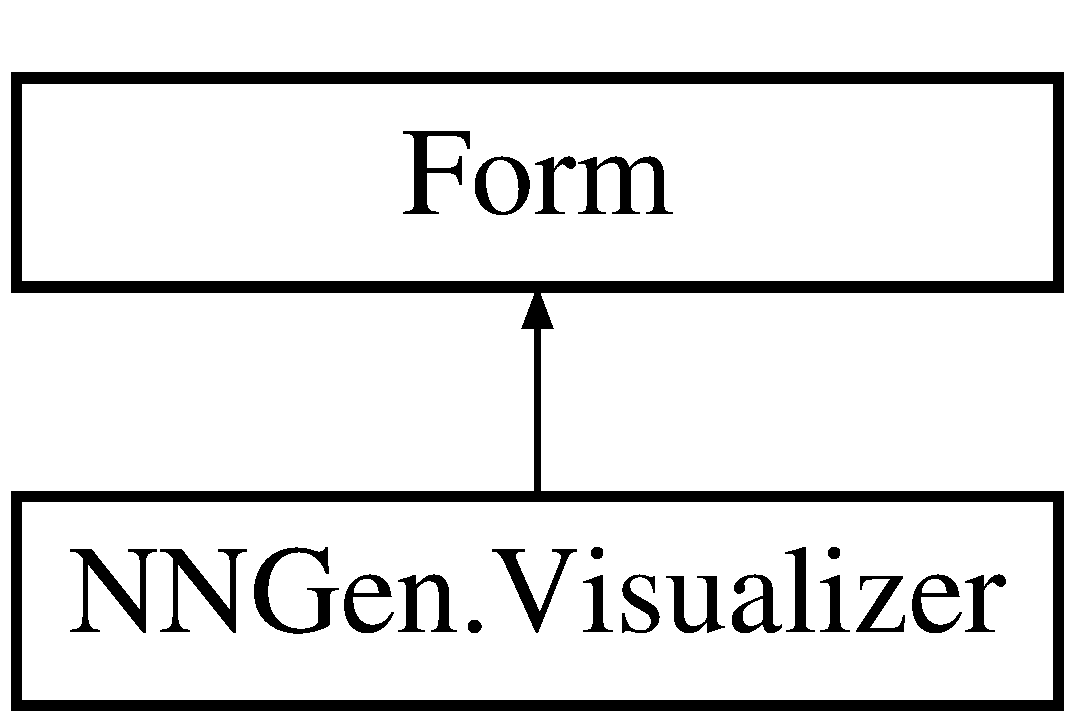
\includegraphics[height=2.000000cm]{class_n_n_gen_1_1_visualizer}
\end{center}
\end{figure}
\subsection*{Public Member Functions}
\begin{DoxyCompactItemize}
\item 
\hyperlink{class_n_n_gen_1_1_visualizer_af5c22f605f7a4ca2a85a61190aed634b}{Visualizer} (\hyperlink{class_n_n_gen_1_1_wizard_controller}{Wizard\+Controller} wc)
\begin{DoxyCompactList}\small\item\em Create a new \hyperlink{class_n_n_gen_1_1_visualizer}{Visualizer} \end{DoxyCompactList}\end{DoxyCompactItemize}
\subsection*{Protected Member Functions}
\begin{DoxyCompactItemize}
\item 
override void \hyperlink{class_n_n_gen_1_1_visualizer_a6a1763644ddf1ec465fbe6ea234d41b0}{Dispose} (bool disposing)
\begin{DoxyCompactList}\small\item\em Clean up any resources being used. \end{DoxyCompactList}\end{DoxyCompactItemize}
\subsection*{Properties}
\begin{DoxyCompactItemize}
\item 
List$<$ \hyperlink{class_n_n_gen_1_1_visualizer_layer}{Visualizer\+Layer} $>$ \hyperlink{class_n_n_gen_1_1_visualizer_a4a5a494c2d58e28febb4a807979e98c1}{layers}\hspace{0.3cm}{\ttfamily  \mbox{[}get\mbox{]}}
\begin{DoxyCompactList}\small\item\em The list of layers that are to be generated by the network \end{DoxyCompactList}\item 
List$<$ \hyperlink{class_n_n_gen_1_1_visualizer_arrow}{Visualizer\+Arrow} $>$ \hyperlink{class_n_n_gen_1_1_visualizer_a63583ab279d0fd3b2b2e5f7e365a46a7}{arrows}\hspace{0.3cm}{\ttfamily  \mbox{[}get\mbox{]}}
\begin{DoxyCompactList}\small\item\em The list of arrows connecting the layers \end{DoxyCompactList}\end{DoxyCompactItemize}


\subsection{Detailed Description}
A for for visualizing the network that is to be generated by the generator 



\subsection{Constructor \& Destructor Documentation}
\hypertarget{class_n_n_gen_1_1_visualizer_af5c22f605f7a4ca2a85a61190aed634b}{}\index{N\+N\+Gen\+::\+Visualizer@{N\+N\+Gen\+::\+Visualizer}!Visualizer@{Visualizer}}
\index{Visualizer@{Visualizer}!N\+N\+Gen\+::\+Visualizer@{N\+N\+Gen\+::\+Visualizer}}
\subsubsection[{Visualizer(\+Wizard\+Controller wc)}]{\setlength{\rightskip}{0pt plus 5cm}N\+N\+Gen.\+Visualizer.\+Visualizer (
\begin{DoxyParamCaption}
\item[{{\bf Wizard\+Controller}}]{wc}
\end{DoxyParamCaption}
)\hspace{0.3cm}{\ttfamily [inline]}}\label{class_n_n_gen_1_1_visualizer_af5c22f605f7a4ca2a85a61190aed634b}


Create a new \hyperlink{class_n_n_gen_1_1_visualizer}{Visualizer} 


\begin{DoxyParams}{Parameters}
{\em wc} & The \hyperlink{class_n_n_gen_1_1_wizard_controller}{Wizard\+Controller} that contains the state of the user\textquotesingle{}s inputs\\
\hline
\end{DoxyParams}


\subsection{Member Function Documentation}
\hypertarget{class_n_n_gen_1_1_visualizer_a6a1763644ddf1ec465fbe6ea234d41b0}{}\index{N\+N\+Gen\+::\+Visualizer@{N\+N\+Gen\+::\+Visualizer}!Dispose@{Dispose}}
\index{Dispose@{Dispose}!N\+N\+Gen\+::\+Visualizer@{N\+N\+Gen\+::\+Visualizer}}
\subsubsection[{Dispose(bool disposing)}]{\setlength{\rightskip}{0pt plus 5cm}override void N\+N\+Gen.\+Visualizer.\+Dispose (
\begin{DoxyParamCaption}
\item[{bool}]{disposing}
\end{DoxyParamCaption}
)\hspace{0.3cm}{\ttfamily [inline]}, {\ttfamily [protected]}}\label{class_n_n_gen_1_1_visualizer_a6a1763644ddf1ec465fbe6ea234d41b0}


Clean up any resources being used. 


\begin{DoxyParams}{Parameters}
{\em disposing} & true if managed resources should be disposed; otherwise, false.\\
\hline
\end{DoxyParams}


\subsection{Property Documentation}
\hypertarget{class_n_n_gen_1_1_visualizer_a63583ab279d0fd3b2b2e5f7e365a46a7}{}\index{N\+N\+Gen\+::\+Visualizer@{N\+N\+Gen\+::\+Visualizer}!arrows@{arrows}}
\index{arrows@{arrows}!N\+N\+Gen\+::\+Visualizer@{N\+N\+Gen\+::\+Visualizer}}
\subsubsection[{arrows}]{\setlength{\rightskip}{0pt plus 5cm}List$<${\bf Visualizer\+Arrow}$>$ N\+N\+Gen.\+Visualizer.\+arrows\hspace{0.3cm}{\ttfamily [get]}}\label{class_n_n_gen_1_1_visualizer_a63583ab279d0fd3b2b2e5f7e365a46a7}


The list of arrows connecting the layers 

\hypertarget{class_n_n_gen_1_1_visualizer_a4a5a494c2d58e28febb4a807979e98c1}{}\index{N\+N\+Gen\+::\+Visualizer@{N\+N\+Gen\+::\+Visualizer}!layers@{layers}}
\index{layers@{layers}!N\+N\+Gen\+::\+Visualizer@{N\+N\+Gen\+::\+Visualizer}}
\subsubsection[{layers}]{\setlength{\rightskip}{0pt plus 5cm}List$<${\bf Visualizer\+Layer}$>$ N\+N\+Gen.\+Visualizer.\+layers\hspace{0.3cm}{\ttfamily [get]}}\label{class_n_n_gen_1_1_visualizer_a4a5a494c2d58e28febb4a807979e98c1}


The list of layers that are to be generated by the network 



The documentation for this class was generated from the following files\+:\begin{DoxyCompactItemize}
\item 
E\+:/\+Documents/\+Visual Studio 2013/\+Projects/\+Neural\+Network/\+N\+N\+Gen/\hyperlink{_visualizer_8cs}{Visualizer.\+cs}\item 
E\+:/\+Documents/\+Visual Studio 2013/\+Projects/\+Neural\+Network/\+N\+N\+Gen/\hyperlink{_visualizer_8_designer_8cs}{Visualizer.\+Designer.\+cs}\end{DoxyCompactItemize}

\hypertarget{class_n_n_gen_1_1_visualizer_arrow}{}\section{N\+N\+Gen.\+Visualizer\+Arrow Class Reference}
\label{class_n_n_gen_1_1_visualizer_arrow}\index{N\+N\+Gen.\+Visualizer\+Arrow@{N\+N\+Gen.\+Visualizer\+Arrow}}


Represents an arrow in the visualizer diagram  


Inheritance diagram for N\+N\+Gen.\+Visualizer\+Arrow\+:\begin{figure}[H]
\begin{center}
\leavevmode
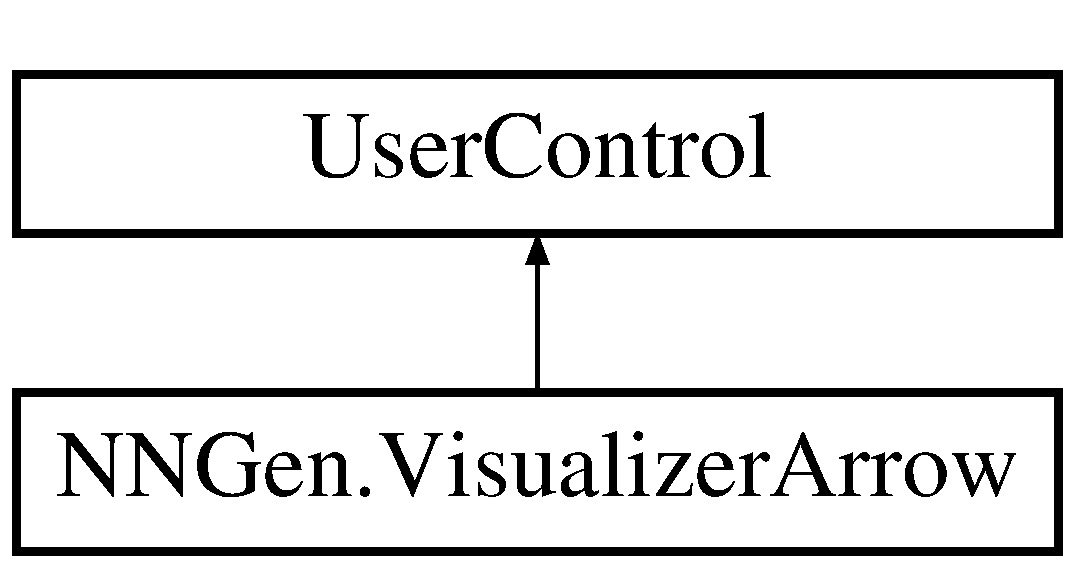
\includegraphics[height=2.000000cm]{class_n_n_gen_1_1_visualizer_arrow}
\end{center}
\end{figure}
\subsection*{Public Member Functions}
\begin{DoxyCompactItemize}
\item 
\hyperlink{class_n_n_gen_1_1_visualizer_arrow_a94d9f0de399b32b1b93f355a6fb545e9}{Visualizer\+Arrow} (int \+\_\+max\+Num\+Int\+Bits, int \+\_\+min\+Num\+Int\+Bits, int \+\_\+num\+Frac\+Bits, int \+\_\+num\+Lines)
\begin{DoxyCompactList}\small\item\em Initialize a \hyperlink{class_n_n_gen_1_1_visualizer_arrow}{Visualizer\+Arrow} \end{DoxyCompactList}\end{DoxyCompactItemize}
\subsection*{Protected Member Functions}
\begin{DoxyCompactItemize}
\item 
override void \hyperlink{class_n_n_gen_1_1_visualizer_arrow_a11971195bff2ff4fd95500b15e8ab579}{On\+Paint} (Paint\+Event\+Args e)
\begin{DoxyCompactList}\small\item\em Paints the \hyperlink{class_n_n_gen_1_1_visualizer_arrow}{Visualizer\+Arrow} on the form \end{DoxyCompactList}\item 
override void \hyperlink{class_n_n_gen_1_1_visualizer_arrow_a272997db19616bfcc87833477ec2a4ff}{Dispose} (bool disposing)
\begin{DoxyCompactList}\small\item\em Clean up any resources being used. \end{DoxyCompactList}\end{DoxyCompactItemize}
\subsection*{Properties}
\begin{DoxyCompactItemize}
\item 
int \hyperlink{class_n_n_gen_1_1_visualizer_arrow_abba2d8807b5dd4b0e531a7e614c015a1}{max\+Num\+Int\+Bits}\hspace{0.3cm}{\ttfamily  \mbox{[}get\mbox{]}}
\begin{DoxyCompactList}\small\item\em The maximal number of integer bits for the layer \end{DoxyCompactList}\item 
int \hyperlink{class_n_n_gen_1_1_visualizer_arrow_a4a80259866c98226a478e827ad55d128}{min\+Num\+Int\+Bits}\hspace{0.3cm}{\ttfamily  \mbox{[}get\mbox{]}}
\begin{DoxyCompactList}\small\item\em The minimal number of fractional bits for the layer \end{DoxyCompactList}\item 
int \hyperlink{class_n_n_gen_1_1_visualizer_arrow_ac9df0a9dfef7922cdb08d23fbe598ede}{num\+Frac\+Bits}\hspace{0.3cm}{\ttfamily  \mbox{[}get\mbox{]}}
\begin{DoxyCompactList}\small\item\em The number of fractional bits for the network \end{DoxyCompactList}\item 
int \hyperlink{class_n_n_gen_1_1_visualizer_arrow_af443e27a47d657b4f030aa51275f8ad2}{num\+Lines}\hspace{0.3cm}{\ttfamily  \mbox{[}get\mbox{]}}
\begin{DoxyCompactList}\small\item\em The number of bus lines between two layers \end{DoxyCompactList}\end{DoxyCompactItemize}


\subsection{Detailed Description}
Represents an arrow in the visualizer diagram 



\subsection{Constructor \& Destructor Documentation}
\hypertarget{class_n_n_gen_1_1_visualizer_arrow_a94d9f0de399b32b1b93f355a6fb545e9}{}\index{N\+N\+Gen\+::\+Visualizer\+Arrow@{N\+N\+Gen\+::\+Visualizer\+Arrow}!Visualizer\+Arrow@{Visualizer\+Arrow}}
\index{Visualizer\+Arrow@{Visualizer\+Arrow}!N\+N\+Gen\+::\+Visualizer\+Arrow@{N\+N\+Gen\+::\+Visualizer\+Arrow}}
\subsubsection[{Visualizer\+Arrow(int \+\_\+max\+Num\+Int\+Bits, int \+\_\+min\+Num\+Int\+Bits, int \+\_\+num\+Frac\+Bits, int \+\_\+num\+Lines)}]{\setlength{\rightskip}{0pt plus 5cm}N\+N\+Gen.\+Visualizer\+Arrow.\+Visualizer\+Arrow (
\begin{DoxyParamCaption}
\item[{int}]{\+\_\+max\+Num\+Int\+Bits, }
\item[{int}]{\+\_\+min\+Num\+Int\+Bits, }
\item[{int}]{\+\_\+num\+Frac\+Bits, }
\item[{int}]{\+\_\+num\+Lines}
\end{DoxyParamCaption}
)\hspace{0.3cm}{\ttfamily [inline]}}\label{class_n_n_gen_1_1_visualizer_arrow_a94d9f0de399b32b1b93f355a6fb545e9}


Initialize a \hyperlink{class_n_n_gen_1_1_visualizer_arrow}{Visualizer\+Arrow} 


\begin{DoxyParams}{Parameters}
{\em \+\_\+max\+Num\+Int\+Bits} & The maximal number of integer bits to display\\
\hline
{\em \+\_\+min\+Num\+Int\+Bits} & The minimal number of integer bits to display\\
\hline
{\em \+\_\+num\+Frac\+Bits} & The number of fractional bits to display\\
\hline
{\em \+\_\+num\+Lines} & The number of bus lines between the two adjacent layers\\
\hline
\end{DoxyParams}


\subsection{Member Function Documentation}
\hypertarget{class_n_n_gen_1_1_visualizer_arrow_a272997db19616bfcc87833477ec2a4ff}{}\index{N\+N\+Gen\+::\+Visualizer\+Arrow@{N\+N\+Gen\+::\+Visualizer\+Arrow}!Dispose@{Dispose}}
\index{Dispose@{Dispose}!N\+N\+Gen\+::\+Visualizer\+Arrow@{N\+N\+Gen\+::\+Visualizer\+Arrow}}
\subsubsection[{Dispose(bool disposing)}]{\setlength{\rightskip}{0pt plus 5cm}override void N\+N\+Gen.\+Visualizer\+Arrow.\+Dispose (
\begin{DoxyParamCaption}
\item[{bool}]{disposing}
\end{DoxyParamCaption}
)\hspace{0.3cm}{\ttfamily [inline]}, {\ttfamily [protected]}}\label{class_n_n_gen_1_1_visualizer_arrow_a272997db19616bfcc87833477ec2a4ff}


Clean up any resources being used. 


\begin{DoxyParams}{Parameters}
{\em disposing} & true if managed resources should be disposed; otherwise, false.\\
\hline
\end{DoxyParams}
\hypertarget{class_n_n_gen_1_1_visualizer_arrow_a11971195bff2ff4fd95500b15e8ab579}{}\index{N\+N\+Gen\+::\+Visualizer\+Arrow@{N\+N\+Gen\+::\+Visualizer\+Arrow}!On\+Paint@{On\+Paint}}
\index{On\+Paint@{On\+Paint}!N\+N\+Gen\+::\+Visualizer\+Arrow@{N\+N\+Gen\+::\+Visualizer\+Arrow}}
\subsubsection[{On\+Paint(\+Paint\+Event\+Args e)}]{\setlength{\rightskip}{0pt plus 5cm}override void N\+N\+Gen.\+Visualizer\+Arrow.\+On\+Paint (
\begin{DoxyParamCaption}
\item[{Paint\+Event\+Args}]{e}
\end{DoxyParamCaption}
)\hspace{0.3cm}{\ttfamily [inline]}, {\ttfamily [protected]}}\label{class_n_n_gen_1_1_visualizer_arrow_a11971195bff2ff4fd95500b15e8ab579}


Paints the \hyperlink{class_n_n_gen_1_1_visualizer_arrow}{Visualizer\+Arrow} on the form 


\begin{DoxyParams}{Parameters}
{\em e} & \\
\hline
\end{DoxyParams}


\subsection{Property Documentation}
\hypertarget{class_n_n_gen_1_1_visualizer_arrow_abba2d8807b5dd4b0e531a7e614c015a1}{}\index{N\+N\+Gen\+::\+Visualizer\+Arrow@{N\+N\+Gen\+::\+Visualizer\+Arrow}!max\+Num\+Int\+Bits@{max\+Num\+Int\+Bits}}
\index{max\+Num\+Int\+Bits@{max\+Num\+Int\+Bits}!N\+N\+Gen\+::\+Visualizer\+Arrow@{N\+N\+Gen\+::\+Visualizer\+Arrow}}
\subsubsection[{max\+Num\+Int\+Bits}]{\setlength{\rightskip}{0pt plus 5cm}int N\+N\+Gen.\+Visualizer\+Arrow.\+max\+Num\+Int\+Bits\hspace{0.3cm}{\ttfamily [get]}}\label{class_n_n_gen_1_1_visualizer_arrow_abba2d8807b5dd4b0e531a7e614c015a1}


The maximal number of integer bits for the layer 

\hypertarget{class_n_n_gen_1_1_visualizer_arrow_a4a80259866c98226a478e827ad55d128}{}\index{N\+N\+Gen\+::\+Visualizer\+Arrow@{N\+N\+Gen\+::\+Visualizer\+Arrow}!min\+Num\+Int\+Bits@{min\+Num\+Int\+Bits}}
\index{min\+Num\+Int\+Bits@{min\+Num\+Int\+Bits}!N\+N\+Gen\+::\+Visualizer\+Arrow@{N\+N\+Gen\+::\+Visualizer\+Arrow}}
\subsubsection[{min\+Num\+Int\+Bits}]{\setlength{\rightskip}{0pt plus 5cm}int N\+N\+Gen.\+Visualizer\+Arrow.\+min\+Num\+Int\+Bits\hspace{0.3cm}{\ttfamily [get]}}\label{class_n_n_gen_1_1_visualizer_arrow_a4a80259866c98226a478e827ad55d128}


The minimal number of fractional bits for the layer 

\hypertarget{class_n_n_gen_1_1_visualizer_arrow_ac9df0a9dfef7922cdb08d23fbe598ede}{}\index{N\+N\+Gen\+::\+Visualizer\+Arrow@{N\+N\+Gen\+::\+Visualizer\+Arrow}!num\+Frac\+Bits@{num\+Frac\+Bits}}
\index{num\+Frac\+Bits@{num\+Frac\+Bits}!N\+N\+Gen\+::\+Visualizer\+Arrow@{N\+N\+Gen\+::\+Visualizer\+Arrow}}
\subsubsection[{num\+Frac\+Bits}]{\setlength{\rightskip}{0pt plus 5cm}int N\+N\+Gen.\+Visualizer\+Arrow.\+num\+Frac\+Bits\hspace{0.3cm}{\ttfamily [get]}}\label{class_n_n_gen_1_1_visualizer_arrow_ac9df0a9dfef7922cdb08d23fbe598ede}


The number of fractional bits for the network 

\hypertarget{class_n_n_gen_1_1_visualizer_arrow_af443e27a47d657b4f030aa51275f8ad2}{}\index{N\+N\+Gen\+::\+Visualizer\+Arrow@{N\+N\+Gen\+::\+Visualizer\+Arrow}!num\+Lines@{num\+Lines}}
\index{num\+Lines@{num\+Lines}!N\+N\+Gen\+::\+Visualizer\+Arrow@{N\+N\+Gen\+::\+Visualizer\+Arrow}}
\subsubsection[{num\+Lines}]{\setlength{\rightskip}{0pt plus 5cm}int N\+N\+Gen.\+Visualizer\+Arrow.\+num\+Lines\hspace{0.3cm}{\ttfamily [get]}}\label{class_n_n_gen_1_1_visualizer_arrow_af443e27a47d657b4f030aa51275f8ad2}


The number of bus lines between two layers 



The documentation for this class was generated from the following files\+:\begin{DoxyCompactItemize}
\item 
E\+:/\+Documents/\+Visual Studio 2013/\+Projects/\+Neural\+Network/\+N\+N\+Gen/\hyperlink{_visualizer_arrow_8cs}{Visualizer\+Arrow.\+cs}\item 
E\+:/\+Documents/\+Visual Studio 2013/\+Projects/\+Neural\+Network/\+N\+N\+Gen/\hyperlink{_visualizer_arrow_8_designer_8cs}{Visualizer\+Arrow.\+Designer.\+cs}\end{DoxyCompactItemize}

\hypertarget{class_n_n_gen_1_1_visualizer_layer}{}\section{N\+N\+Gen.\+Visualizer\+Layer Class Reference}
\label{class_n_n_gen_1_1_visualizer_layer}\index{N\+N\+Gen.\+Visualizer\+Layer@{N\+N\+Gen.\+Visualizer\+Layer}}


A representation of a layer in the \hyperlink{class_n_n_gen_1_1_visualizer}{Visualizer}  


Inheritance diagram for N\+N\+Gen.\+Visualizer\+Layer\+:\begin{figure}[H]
\begin{center}
\leavevmode
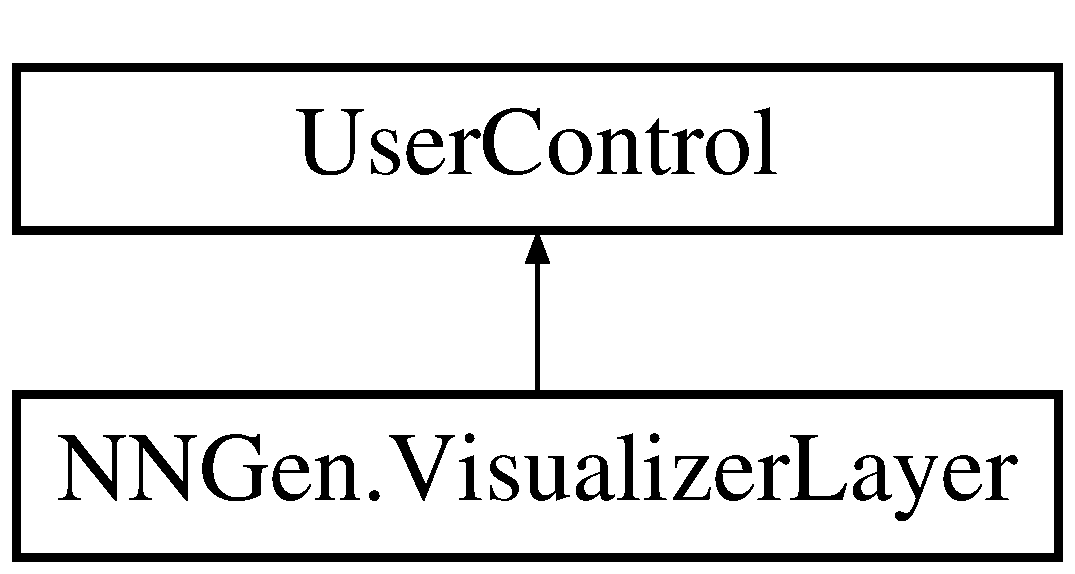
\includegraphics[height=2.000000cm]{class_n_n_gen_1_1_visualizer_layer}
\end{center}
\end{figure}
\subsection*{Public Member Functions}
\begin{DoxyCompactItemize}
\item 
\hyperlink{class_n_n_gen_1_1_visualizer_layer_a68a8bef64c4066c35865f8f505e6afe7}{Visualizer\+Layer} (int \+\_\+num\+Neurons, \hyperlink{class_n_n_gen_1_1_async_neuron_afe8460a52808d1587cbcc0a8e4e23b64}{Async\+Neuron.\+Neuron\+Activation\+Type} \+\_\+async\+Activation\+Type, \hyperlink{class_n_n_gen_1_1_transfer_function_wrapper_aa338ffadb8fcdf76df75419374a51ff6}{Transfer\+Function\+Wrapper.\+Memory\+Activation\+Type} \+\_\+sync\+Activation\+Type, bool \+\_\+is\+Synchronous, string \+\_\+layer\+Name, bool \+\_\+is\+First\+Layer)
\begin{DoxyCompactList}\small\item\em Create a \hyperlink{class_n_n_gen_1_1_visualizer_layer}{Visualizer\+Layer} \end{DoxyCompactList}\end{DoxyCompactItemize}
\subsection*{Protected Member Functions}
\begin{DoxyCompactItemize}
\item 
override void \hyperlink{class_n_n_gen_1_1_visualizer_layer_ab129e028f30623f2377b82d2e3f1c7ed}{On\+Paint} (Paint\+Event\+Args e)
\begin{DoxyCompactList}\small\item\em Paints the form \end{DoxyCompactList}\item 
override void \hyperlink{class_n_n_gen_1_1_visualizer_layer_a94a79048a1188b72705c77503a801008}{Dispose} (bool disposing)
\begin{DoxyCompactList}\small\item\em Clean up any resources being used. \end{DoxyCompactList}\end{DoxyCompactItemize}
\subsection*{Properties}
\begin{DoxyCompactItemize}
\item 
int \hyperlink{class_n_n_gen_1_1_visualizer_layer_aaf9ed8af2561bf8203a81cba1bf324be}{num\+Neurons}\hspace{0.3cm}{\ttfamily  \mbox{[}get\mbox{]}}
\begin{DoxyCompactList}\small\item\em The number of neurons in the network \end{DoxyCompactList}\item 
\hyperlink{class_n_n_gen_1_1_async_neuron_afe8460a52808d1587cbcc0a8e4e23b64}{Async\+Neuron.\+Neuron\+Activation\+Type} \hyperlink{class_n_n_gen_1_1_visualizer_layer_ace064a62dbac8d9ba6ab091f3275f809}{async\+Activation\+Type}\hspace{0.3cm}{\ttfamily  \mbox{[}get\mbox{]}}
\begin{DoxyCompactList}\small\item\em For asyncronous networks, the activation type of the layer \end{DoxyCompactList}\item 
\hyperlink{class_n_n_gen_1_1_transfer_function_wrapper_aa338ffadb8fcdf76df75419374a51ff6}{Transfer\+Function\+Wrapper.\+Memory\+Activation\+Type} \hyperlink{class_n_n_gen_1_1_visualizer_layer_a4e3138e1ee1d9220ff8c53d0ac860f14}{sync\+Activation\+Type}\hspace{0.3cm}{\ttfamily  \mbox{[}get\mbox{]}}
\begin{DoxyCompactList}\small\item\em For syncronous networks, the activatino type of the layer \end{DoxyCompactList}\item 
string \hyperlink{class_n_n_gen_1_1_visualizer_layer_a2f19de515420357a18d890cec3a3e43b}{activation\+Type\+\_\+string}\hspace{0.3cm}{\ttfamily  \mbox{[}get\mbox{]}}
\begin{DoxyCompactList}\small\item\em A human-\/readable string representation of the activation type \end{DoxyCompactList}\item 
string \hyperlink{class_n_n_gen_1_1_visualizer_layer_adf0f91a6cf7dd357ff14b44f5c967a5f}{layer\+Name}\hspace{0.3cm}{\ttfamily  \mbox{[}get\mbox{]}}
\begin{DoxyCompactList}\small\item\em The name of the layer \end{DoxyCompactList}\item 
bool \hyperlink{class_n_n_gen_1_1_visualizer_layer_ae0cf894b1f6ca60a8cbcfd3e862763f7}{is\+Synchronous}\hspace{0.3cm}{\ttfamily  \mbox{[}get\mbox{]}}
\begin{DoxyCompactList}\small\item\em Whether the layer is synchronous \end{DoxyCompactList}\item 
bool \hyperlink{class_n_n_gen_1_1_visualizer_layer_a260e665a2e4ec4651ff796c4de269eca}{is\+First\+Layer}\hspace{0.3cm}{\ttfamily  \mbox{[}get\mbox{]}}
\begin{DoxyCompactList}\small\item\em Whether the layer is the first layer in the network \end{DoxyCompactList}\end{DoxyCompactItemize}


\subsection{Detailed Description}
A representation of a layer in the \hyperlink{class_n_n_gen_1_1_visualizer}{Visualizer} 



\subsection{Constructor \& Destructor Documentation}
\hypertarget{class_n_n_gen_1_1_visualizer_layer_a68a8bef64c4066c35865f8f505e6afe7}{}\index{N\+N\+Gen\+::\+Visualizer\+Layer@{N\+N\+Gen\+::\+Visualizer\+Layer}!Visualizer\+Layer@{Visualizer\+Layer}}
\index{Visualizer\+Layer@{Visualizer\+Layer}!N\+N\+Gen\+::\+Visualizer\+Layer@{N\+N\+Gen\+::\+Visualizer\+Layer}}
\subsubsection[{Visualizer\+Layer(int \+\_\+num\+Neurons, Async\+Neuron.\+Neuron\+Activation\+Type \+\_\+async\+Activation\+Type, Transfer\+Function\+Wrapper.\+Memory\+Activation\+Type \+\_\+sync\+Activation\+Type, bool \+\_\+is\+Synchronous, string \+\_\+layer\+Name, bool \+\_\+is\+First\+Layer)}]{\setlength{\rightskip}{0pt plus 5cm}N\+N\+Gen.\+Visualizer\+Layer.\+Visualizer\+Layer (
\begin{DoxyParamCaption}
\item[{int}]{\+\_\+num\+Neurons, }
\item[{{\bf Async\+Neuron.\+Neuron\+Activation\+Type}}]{\+\_\+async\+Activation\+Type, }
\item[{{\bf Transfer\+Function\+Wrapper.\+Memory\+Activation\+Type}}]{\+\_\+sync\+Activation\+Type, }
\item[{bool}]{\+\_\+is\+Synchronous, }
\item[{string}]{\+\_\+layer\+Name, }
\item[{bool}]{\+\_\+is\+First\+Layer}
\end{DoxyParamCaption}
)\hspace{0.3cm}{\ttfamily [inline]}}\label{class_n_n_gen_1_1_visualizer_layer_a68a8bef64c4066c35865f8f505e6afe7}


Create a \hyperlink{class_n_n_gen_1_1_visualizer_layer}{Visualizer\+Layer} 


\begin{DoxyParams}{Parameters}
{\em \+\_\+num\+Neurons} & The number of neurons in the layer\\
\hline
{\em \+\_\+async\+Activation\+Type} & For an asynchronous network, the activation type. Ignored for synchronous networks\\
\hline
{\em \+\_\+sync\+Activation\+Type} & For a synchronous network, the activation type. Ignored for asynchronous networks\\
\hline
{\em \+\_\+is\+Synchronous} & A flag determining whether the network is synchronous or not\\
\hline
{\em \+\_\+layer\+Name} & The name of the layer\\
\hline
{\em \+\_\+is\+First\+Layer} & A flag representing whether this layer is the first layer in the network. Used to mask the activation type\\
\hline
\end{DoxyParams}


\subsection{Member Function Documentation}
\hypertarget{class_n_n_gen_1_1_visualizer_layer_a94a79048a1188b72705c77503a801008}{}\index{N\+N\+Gen\+::\+Visualizer\+Layer@{N\+N\+Gen\+::\+Visualizer\+Layer}!Dispose@{Dispose}}
\index{Dispose@{Dispose}!N\+N\+Gen\+::\+Visualizer\+Layer@{N\+N\+Gen\+::\+Visualizer\+Layer}}
\subsubsection[{Dispose(bool disposing)}]{\setlength{\rightskip}{0pt plus 5cm}override void N\+N\+Gen.\+Visualizer\+Layer.\+Dispose (
\begin{DoxyParamCaption}
\item[{bool}]{disposing}
\end{DoxyParamCaption}
)\hspace{0.3cm}{\ttfamily [inline]}, {\ttfamily [protected]}}\label{class_n_n_gen_1_1_visualizer_layer_a94a79048a1188b72705c77503a801008}


Clean up any resources being used. 


\begin{DoxyParams}{Parameters}
{\em disposing} & true if managed resources should be disposed; otherwise, false.\\
\hline
\end{DoxyParams}
\hypertarget{class_n_n_gen_1_1_visualizer_layer_ab129e028f30623f2377b82d2e3f1c7ed}{}\index{N\+N\+Gen\+::\+Visualizer\+Layer@{N\+N\+Gen\+::\+Visualizer\+Layer}!On\+Paint@{On\+Paint}}
\index{On\+Paint@{On\+Paint}!N\+N\+Gen\+::\+Visualizer\+Layer@{N\+N\+Gen\+::\+Visualizer\+Layer}}
\subsubsection[{On\+Paint(\+Paint\+Event\+Args e)}]{\setlength{\rightskip}{0pt plus 5cm}override void N\+N\+Gen.\+Visualizer\+Layer.\+On\+Paint (
\begin{DoxyParamCaption}
\item[{Paint\+Event\+Args}]{e}
\end{DoxyParamCaption}
)\hspace{0.3cm}{\ttfamily [inline]}, {\ttfamily [protected]}}\label{class_n_n_gen_1_1_visualizer_layer_ab129e028f30623f2377b82d2e3f1c7ed}


Paints the form 


\begin{DoxyParams}{Parameters}
{\em e} & \\
\hline
\end{DoxyParams}


\subsection{Property Documentation}
\hypertarget{class_n_n_gen_1_1_visualizer_layer_a2f19de515420357a18d890cec3a3e43b}{}\index{N\+N\+Gen\+::\+Visualizer\+Layer@{N\+N\+Gen\+::\+Visualizer\+Layer}!activation\+Type\+\_\+string@{activation\+Type\+\_\+string}}
\index{activation\+Type\+\_\+string@{activation\+Type\+\_\+string}!N\+N\+Gen\+::\+Visualizer\+Layer@{N\+N\+Gen\+::\+Visualizer\+Layer}}
\subsubsection[{activation\+Type\+\_\+string}]{\setlength{\rightskip}{0pt plus 5cm}string N\+N\+Gen.\+Visualizer\+Layer.\+activation\+Type\+\_\+string\hspace{0.3cm}{\ttfamily [get]}}\label{class_n_n_gen_1_1_visualizer_layer_a2f19de515420357a18d890cec3a3e43b}


A human-\/readable string representation of the activation type 

\hypertarget{class_n_n_gen_1_1_visualizer_layer_ace064a62dbac8d9ba6ab091f3275f809}{}\index{N\+N\+Gen\+::\+Visualizer\+Layer@{N\+N\+Gen\+::\+Visualizer\+Layer}!async\+Activation\+Type@{async\+Activation\+Type}}
\index{async\+Activation\+Type@{async\+Activation\+Type}!N\+N\+Gen\+::\+Visualizer\+Layer@{N\+N\+Gen\+::\+Visualizer\+Layer}}
\subsubsection[{async\+Activation\+Type}]{\setlength{\rightskip}{0pt plus 5cm}{\bf Async\+Neuron.\+Neuron\+Activation\+Type} N\+N\+Gen.\+Visualizer\+Layer.\+async\+Activation\+Type\hspace{0.3cm}{\ttfamily [get]}}\label{class_n_n_gen_1_1_visualizer_layer_ace064a62dbac8d9ba6ab091f3275f809}


For asyncronous networks, the activation type of the layer 

\hypertarget{class_n_n_gen_1_1_visualizer_layer_a260e665a2e4ec4651ff796c4de269eca}{}\index{N\+N\+Gen\+::\+Visualizer\+Layer@{N\+N\+Gen\+::\+Visualizer\+Layer}!is\+First\+Layer@{is\+First\+Layer}}
\index{is\+First\+Layer@{is\+First\+Layer}!N\+N\+Gen\+::\+Visualizer\+Layer@{N\+N\+Gen\+::\+Visualizer\+Layer}}
\subsubsection[{is\+First\+Layer}]{\setlength{\rightskip}{0pt plus 5cm}bool N\+N\+Gen.\+Visualizer\+Layer.\+is\+First\+Layer\hspace{0.3cm}{\ttfamily [get]}}\label{class_n_n_gen_1_1_visualizer_layer_a260e665a2e4ec4651ff796c4de269eca}


Whether the layer is the first layer in the network 

\hypertarget{class_n_n_gen_1_1_visualizer_layer_ae0cf894b1f6ca60a8cbcfd3e862763f7}{}\index{N\+N\+Gen\+::\+Visualizer\+Layer@{N\+N\+Gen\+::\+Visualizer\+Layer}!is\+Synchronous@{is\+Synchronous}}
\index{is\+Synchronous@{is\+Synchronous}!N\+N\+Gen\+::\+Visualizer\+Layer@{N\+N\+Gen\+::\+Visualizer\+Layer}}
\subsubsection[{is\+Synchronous}]{\setlength{\rightskip}{0pt plus 5cm}bool N\+N\+Gen.\+Visualizer\+Layer.\+is\+Synchronous\hspace{0.3cm}{\ttfamily [get]}}\label{class_n_n_gen_1_1_visualizer_layer_ae0cf894b1f6ca60a8cbcfd3e862763f7}


Whether the layer is synchronous 

\hypertarget{class_n_n_gen_1_1_visualizer_layer_adf0f91a6cf7dd357ff14b44f5c967a5f}{}\index{N\+N\+Gen\+::\+Visualizer\+Layer@{N\+N\+Gen\+::\+Visualizer\+Layer}!layer\+Name@{layer\+Name}}
\index{layer\+Name@{layer\+Name}!N\+N\+Gen\+::\+Visualizer\+Layer@{N\+N\+Gen\+::\+Visualizer\+Layer}}
\subsubsection[{layer\+Name}]{\setlength{\rightskip}{0pt plus 5cm}string N\+N\+Gen.\+Visualizer\+Layer.\+layer\+Name\hspace{0.3cm}{\ttfamily [get]}}\label{class_n_n_gen_1_1_visualizer_layer_adf0f91a6cf7dd357ff14b44f5c967a5f}


The name of the layer 

\hypertarget{class_n_n_gen_1_1_visualizer_layer_aaf9ed8af2561bf8203a81cba1bf324be}{}\index{N\+N\+Gen\+::\+Visualizer\+Layer@{N\+N\+Gen\+::\+Visualizer\+Layer}!num\+Neurons@{num\+Neurons}}
\index{num\+Neurons@{num\+Neurons}!N\+N\+Gen\+::\+Visualizer\+Layer@{N\+N\+Gen\+::\+Visualizer\+Layer}}
\subsubsection[{num\+Neurons}]{\setlength{\rightskip}{0pt plus 5cm}int N\+N\+Gen.\+Visualizer\+Layer.\+num\+Neurons\hspace{0.3cm}{\ttfamily [get]}}\label{class_n_n_gen_1_1_visualizer_layer_aaf9ed8af2561bf8203a81cba1bf324be}


The number of neurons in the network 

\hypertarget{class_n_n_gen_1_1_visualizer_layer_a4e3138e1ee1d9220ff8c53d0ac860f14}{}\index{N\+N\+Gen\+::\+Visualizer\+Layer@{N\+N\+Gen\+::\+Visualizer\+Layer}!sync\+Activation\+Type@{sync\+Activation\+Type}}
\index{sync\+Activation\+Type@{sync\+Activation\+Type}!N\+N\+Gen\+::\+Visualizer\+Layer@{N\+N\+Gen\+::\+Visualizer\+Layer}}
\subsubsection[{sync\+Activation\+Type}]{\setlength{\rightskip}{0pt plus 5cm}{\bf Transfer\+Function\+Wrapper.\+Memory\+Activation\+Type} N\+N\+Gen.\+Visualizer\+Layer.\+sync\+Activation\+Type\hspace{0.3cm}{\ttfamily [get]}}\label{class_n_n_gen_1_1_visualizer_layer_a4e3138e1ee1d9220ff8c53d0ac860f14}


For syncronous networks, the activatino type of the layer 



The documentation for this class was generated from the following files\+:\begin{DoxyCompactItemize}
\item 
E\+:/\+Documents/\+Visual Studio 2013/\+Projects/\+Neural\+Network/\+N\+N\+Gen/\hyperlink{_visualizer_layer_8cs}{Visualizer\+Layer.\+cs}\item 
E\+:/\+Documents/\+Visual Studio 2013/\+Projects/\+Neural\+Network/\+N\+N\+Gen/\hyperlink{_visualizer_layer_8_designer_8cs}{Visualizer\+Layer.\+Designer.\+cs}\end{DoxyCompactItemize}

\hypertarget{class_n_n_gen_1_1_weight_memory}{}\section{N\+N\+Gen.\+Weight\+Memory Class Reference}
\label{class_n_n_gen_1_1_weight_memory}\index{N\+N\+Gen.\+Weight\+Memory@{N\+N\+Gen.\+Weight\+Memory}}


An entity that infers memory intended to be used for initializing a neural network  


Inheritance diagram for N\+N\+Gen.\+Weight\+Memory\+:\begin{figure}[H]
\begin{center}
\leavevmode
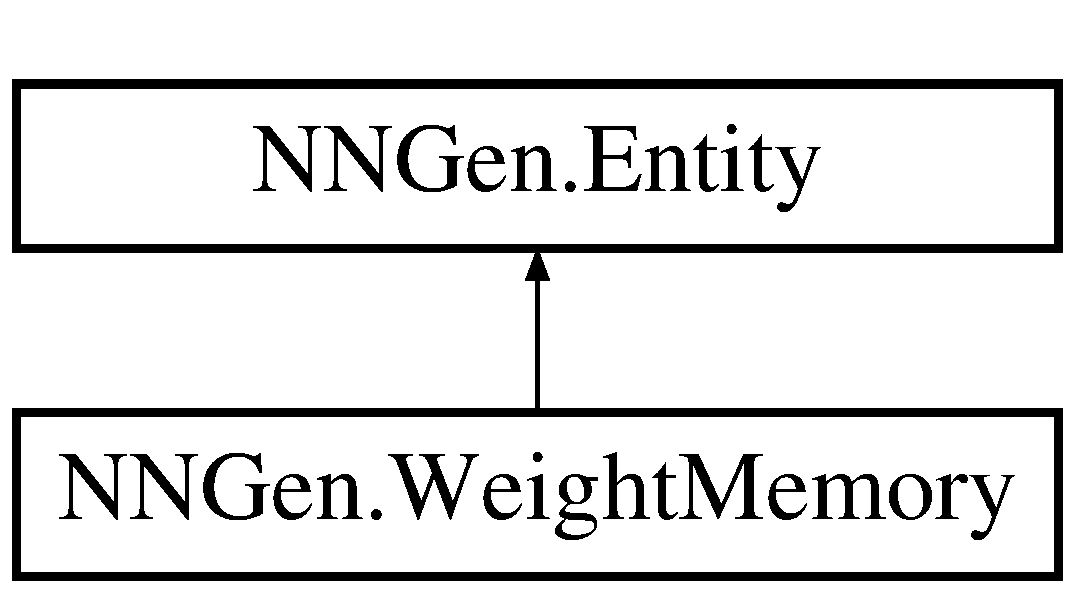
\includegraphics[height=2.000000cm]{class_n_n_gen_1_1_weight_memory}
\end{center}
\end{figure}
\subsection*{Public Member Functions}
\begin{DoxyCompactItemize}
\item 
\hyperlink{class_n_n_gen_1_1_weight_memory_a5be8cc5e6e42aedf41967c299efd75cf}{Weight\+Memory} (int \+\_\+num\+Int\+Bits, int \+\_\+num\+Frac\+Bits, List$<$ double $>$ \+\_\+weights)
\begin{DoxyCompactList}\small\item\em Initializes the entity \end{DoxyCompactList}\item 
override string \hyperlink{class_n_n_gen_1_1_weight_memory_a000cfa9b5dd1d41042ed77dbad178aeb}{get\+Name} ()
\begin{DoxyCompactList}\small\item\em Returns the name of the entity \end{DoxyCompactList}\item 
override \hyperlink{class_n_n_gen_1_1_port}{Port}\mbox{[}$\,$\mbox{]} \hyperlink{class_n_n_gen_1_1_weight_memory_a0f80fe3a06082c2e238f1c7b552c723d}{get\+Input\+Ports} ()
\begin{DoxyCompactList}\small\item\em Returns the inputs to the device \end{DoxyCompactList}\item 
override \hyperlink{class_n_n_gen_1_1_port}{Port}\mbox{[}$\,$\mbox{]} \hyperlink{class_n_n_gen_1_1_weight_memory_a96cae98991fe72526efcc94aa27c3294}{get\+Output\+Ports} ()
\begin{DoxyCompactList}\small\item\em Returns the outputs to the device \end{DoxyCompactList}\item 
override \hyperlink{class_n_n_gen_1_1_signal}{Signal}\mbox{[}$\,$\mbox{]} \hyperlink{class_n_n_gen_1_1_weight_memory_a7166780b7824c585e92da81172aaba22}{get\+Internal\+Signals} ()
\begin{DoxyCompactList}\small\item\em Returns the internal signals for the device \end{DoxyCompactList}\item 
override bool \hyperlink{class_n_n_gen_1_1_weight_memory_a638a0f1ce7d8f3983ef0a0beb59e887d}{write\+V\+H\+D\+L} (string file)
\begin{DoxyCompactList}\small\item\em Writes the .vhd files necessary to compile this entity. All other necessary entities (i.\+e. neurons, thresholding functions, etc.) will also be written when this function returns \end{DoxyCompactList}\end{DoxyCompactItemize}
\subsection*{Properties}
\begin{DoxyCompactItemize}
\item 
\hyperlink{class_n_n_gen_1_1_port}{Port} \hyperlink{class_n_n_gen_1_1_weight_memory_afd016b54cfb5b510f02e5e9d47dd0292}{clk}\hspace{0.3cm}{\ttfamily  \mbox{[}get\mbox{]}}
\begin{DoxyCompactList}\small\item\em The clock signal. The memory device output is rising-\/edge registered \end{DoxyCompactList}\item 
\hyperlink{class_n_n_gen_1_1_port}{Port} \hyperlink{class_n_n_gen_1_1_weight_memory_a86f72ffc5ccc873778854121075a52da}{addr}\hspace{0.3cm}{\ttfamily  \mbox{[}get\mbox{]}}
\begin{DoxyCompactList}\small\item\em The address lines for the memory \end{DoxyCompactList}\item 
\hyperlink{class_n_n_gen_1_1_port}{Port} \hyperlink{class_n_n_gen_1_1_weight_memory_a83826d4cceec2993daebe283204e12b6}{data}\hspace{0.3cm}{\ttfamily  \mbox{[}get\mbox{]}}
\begin{DoxyCompactList}\small\item\em Memory output. On rising edge, the contents of memory pointed to by \char`\"{}addr\char`\"{} will appear on \char`\"{}q\char`\"{} \end{DoxyCompactList}\item 
List$<$ string $>$ \hyperlink{class_n_n_gen_1_1_weight_memory_a969c7f7f162b75653ff1cb94eb1d11a8}{weights\+\_\+str}\hspace{0.3cm}{\ttfamily  \mbox{[}get\mbox{]}}
\begin{DoxyCompactList}\small\item\em The initialization values for the memory. the i-\/th element will appear in the i-\/th address on startup. \end{DoxyCompactList}\item 
string \hyperlink{class_n_n_gen_1_1_weight_memory_a4b89726fb6f1303d0b898f29d28545cc}{name}\hspace{0.3cm}{\ttfamily  \mbox{[}get\mbox{]}}
\begin{DoxyCompactList}\small\item\em The name of the entity \end{DoxyCompactList}\end{DoxyCompactItemize}


\subsection{Detailed Description}
An entity that infers memory intended to be used for initializing a neural network 



\subsection{Constructor \& Destructor Documentation}
\hypertarget{class_n_n_gen_1_1_weight_memory_a5be8cc5e6e42aedf41967c299efd75cf}{}\index{N\+N\+Gen\+::\+Weight\+Memory@{N\+N\+Gen\+::\+Weight\+Memory}!Weight\+Memory@{Weight\+Memory}}
\index{Weight\+Memory@{Weight\+Memory}!N\+N\+Gen\+::\+Weight\+Memory@{N\+N\+Gen\+::\+Weight\+Memory}}
\subsubsection[{Weight\+Memory(int \+\_\+num\+Int\+Bits, int \+\_\+num\+Frac\+Bits, List$<$ double $>$ \+\_\+weights)}]{\setlength{\rightskip}{0pt plus 5cm}N\+N\+Gen.\+Weight\+Memory.\+Weight\+Memory (
\begin{DoxyParamCaption}
\item[{int}]{\+\_\+num\+Int\+Bits, }
\item[{int}]{\+\_\+num\+Frac\+Bits, }
\item[{List$<$ double $>$}]{\+\_\+weights}
\end{DoxyParamCaption}
)\hspace{0.3cm}{\ttfamily [inline]}}\label{class_n_n_gen_1_1_weight_memory_a5be8cc5e6e42aedf41967c299efd75cf}


Initializes the entity 


\begin{DoxyParams}{Parameters}
{\em \+\_\+num\+Int\+Bits} & The number of integer bits to be used on the output bus\\
\hline
{\em \+\_\+num\+Frac\+Bits} & The number of fractional bits to be used on the output bus\\
\hline
{\em \+\_\+weights} & The list of startup weights (see weights\+\_\+str)\\
\hline
\end{DoxyParams}


\subsection{Member Function Documentation}
\hypertarget{class_n_n_gen_1_1_weight_memory_a0f80fe3a06082c2e238f1c7b552c723d}{}\index{N\+N\+Gen\+::\+Weight\+Memory@{N\+N\+Gen\+::\+Weight\+Memory}!get\+Input\+Ports@{get\+Input\+Ports}}
\index{get\+Input\+Ports@{get\+Input\+Ports}!N\+N\+Gen\+::\+Weight\+Memory@{N\+N\+Gen\+::\+Weight\+Memory}}
\subsubsection[{get\+Input\+Ports()}]{\setlength{\rightskip}{0pt plus 5cm}override {\bf Port} \mbox{[}$\,$\mbox{]} N\+N\+Gen.\+Weight\+Memory.\+get\+Input\+Ports (
\begin{DoxyParamCaption}
{}
\end{DoxyParamCaption}
)\hspace{0.3cm}{\ttfamily [inline]}, {\ttfamily [virtual]}}\label{class_n_n_gen_1_1_weight_memory_a0f80fe3a06082c2e238f1c7b552c723d}


Returns the inputs to the device 

\begin{DoxyReturn}{Returns}
The inputs to the device
\end{DoxyReturn}


Implements \hyperlink{class_n_n_gen_1_1_entity_a01239f05c9efa61ec9e6a29cb2eaad50}{N\+N\+Gen.\+Entity}.

\hypertarget{class_n_n_gen_1_1_weight_memory_a7166780b7824c585e92da81172aaba22}{}\index{N\+N\+Gen\+::\+Weight\+Memory@{N\+N\+Gen\+::\+Weight\+Memory}!get\+Internal\+Signals@{get\+Internal\+Signals}}
\index{get\+Internal\+Signals@{get\+Internal\+Signals}!N\+N\+Gen\+::\+Weight\+Memory@{N\+N\+Gen\+::\+Weight\+Memory}}
\subsubsection[{get\+Internal\+Signals()}]{\setlength{\rightskip}{0pt plus 5cm}override {\bf Signal} \mbox{[}$\,$\mbox{]} N\+N\+Gen.\+Weight\+Memory.\+get\+Internal\+Signals (
\begin{DoxyParamCaption}
{}
\end{DoxyParamCaption}
)\hspace{0.3cm}{\ttfamily [inline]}, {\ttfamily [virtual]}}\label{class_n_n_gen_1_1_weight_memory_a7166780b7824c585e92da81172aaba22}


Returns the internal signals for the device 

\begin{DoxyReturn}{Returns}
The internal signals for the device
\end{DoxyReturn}


Implements \hyperlink{class_n_n_gen_1_1_entity_a62feb80e95ec84c650ea17bd53f0d510}{N\+N\+Gen.\+Entity}.

\hypertarget{class_n_n_gen_1_1_weight_memory_a000cfa9b5dd1d41042ed77dbad178aeb}{}\index{N\+N\+Gen\+::\+Weight\+Memory@{N\+N\+Gen\+::\+Weight\+Memory}!get\+Name@{get\+Name}}
\index{get\+Name@{get\+Name}!N\+N\+Gen\+::\+Weight\+Memory@{N\+N\+Gen\+::\+Weight\+Memory}}
\subsubsection[{get\+Name()}]{\setlength{\rightskip}{0pt plus 5cm}override string N\+N\+Gen.\+Weight\+Memory.\+get\+Name (
\begin{DoxyParamCaption}
{}
\end{DoxyParamCaption}
)\hspace{0.3cm}{\ttfamily [inline]}, {\ttfamily [virtual]}}\label{class_n_n_gen_1_1_weight_memory_a000cfa9b5dd1d41042ed77dbad178aeb}


Returns the name of the entity 

\begin{DoxyReturn}{Returns}
The name of the entity
\end{DoxyReturn}


Implements \hyperlink{class_n_n_gen_1_1_entity_a9f25d1070c9ab8ad343c28443e62e6f2}{N\+N\+Gen.\+Entity}.

\hypertarget{class_n_n_gen_1_1_weight_memory_a96cae98991fe72526efcc94aa27c3294}{}\index{N\+N\+Gen\+::\+Weight\+Memory@{N\+N\+Gen\+::\+Weight\+Memory}!get\+Output\+Ports@{get\+Output\+Ports}}
\index{get\+Output\+Ports@{get\+Output\+Ports}!N\+N\+Gen\+::\+Weight\+Memory@{N\+N\+Gen\+::\+Weight\+Memory}}
\subsubsection[{get\+Output\+Ports()}]{\setlength{\rightskip}{0pt plus 5cm}override {\bf Port} \mbox{[}$\,$\mbox{]} N\+N\+Gen.\+Weight\+Memory.\+get\+Output\+Ports (
\begin{DoxyParamCaption}
{}
\end{DoxyParamCaption}
)\hspace{0.3cm}{\ttfamily [inline]}, {\ttfamily [virtual]}}\label{class_n_n_gen_1_1_weight_memory_a96cae98991fe72526efcc94aa27c3294}


Returns the outputs to the device 

\begin{DoxyReturn}{Returns}
The outputs to the device
\end{DoxyReturn}


Implements \hyperlink{class_n_n_gen_1_1_entity_ace06368087778e254a5048c7d28747be}{N\+N\+Gen.\+Entity}.

\hypertarget{class_n_n_gen_1_1_weight_memory_a638a0f1ce7d8f3983ef0a0beb59e887d}{}\index{N\+N\+Gen\+::\+Weight\+Memory@{N\+N\+Gen\+::\+Weight\+Memory}!write\+V\+H\+D\+L@{write\+V\+H\+D\+L}}
\index{write\+V\+H\+D\+L@{write\+V\+H\+D\+L}!N\+N\+Gen\+::\+Weight\+Memory@{N\+N\+Gen\+::\+Weight\+Memory}}
\subsubsection[{write\+V\+H\+D\+L(string file)}]{\setlength{\rightskip}{0pt plus 5cm}override bool N\+N\+Gen.\+Weight\+Memory.\+write\+V\+H\+D\+L (
\begin{DoxyParamCaption}
\item[{string}]{file}
\end{DoxyParamCaption}
)\hspace{0.3cm}{\ttfamily [inline]}, {\ttfamily [virtual]}}\label{class_n_n_gen_1_1_weight_memory_a638a0f1ce7d8f3983ef0a0beb59e887d}


Writes the .vhd files necessary to compile this entity. All other necessary entities (i.\+e. neurons, thresholding functions, etc.) will also be written when this function returns 


\begin{DoxyParams}{Parameters}
{\em file} & The file path in which to write the files (do N\+O\+T include \char`\"{}...\+name.\+vhd\char`\"{}\\
\hline
\end{DoxyParams}
\begin{DoxyReturn}{Returns}
true if the files were written successfully, false otherwise
\end{DoxyReturn}


Implements \hyperlink{class_n_n_gen_1_1_entity_a1111d498446be08b20583b9625893a52}{N\+N\+Gen.\+Entity}.



\subsection{Property Documentation}
\hypertarget{class_n_n_gen_1_1_weight_memory_a86f72ffc5ccc873778854121075a52da}{}\index{N\+N\+Gen\+::\+Weight\+Memory@{N\+N\+Gen\+::\+Weight\+Memory}!addr@{addr}}
\index{addr@{addr}!N\+N\+Gen\+::\+Weight\+Memory@{N\+N\+Gen\+::\+Weight\+Memory}}
\subsubsection[{addr}]{\setlength{\rightskip}{0pt plus 5cm}{\bf Port} N\+N\+Gen.\+Weight\+Memory.\+addr\hspace{0.3cm}{\ttfamily [get]}}\label{class_n_n_gen_1_1_weight_memory_a86f72ffc5ccc873778854121075a52da}


The address lines for the memory 

\hypertarget{class_n_n_gen_1_1_weight_memory_afd016b54cfb5b510f02e5e9d47dd0292}{}\index{N\+N\+Gen\+::\+Weight\+Memory@{N\+N\+Gen\+::\+Weight\+Memory}!clk@{clk}}
\index{clk@{clk}!N\+N\+Gen\+::\+Weight\+Memory@{N\+N\+Gen\+::\+Weight\+Memory}}
\subsubsection[{clk}]{\setlength{\rightskip}{0pt plus 5cm}{\bf Port} N\+N\+Gen.\+Weight\+Memory.\+clk\hspace{0.3cm}{\ttfamily [get]}}\label{class_n_n_gen_1_1_weight_memory_afd016b54cfb5b510f02e5e9d47dd0292}


The clock signal. The memory device output is rising-\/edge registered 

\hypertarget{class_n_n_gen_1_1_weight_memory_a83826d4cceec2993daebe283204e12b6}{}\index{N\+N\+Gen\+::\+Weight\+Memory@{N\+N\+Gen\+::\+Weight\+Memory}!data@{data}}
\index{data@{data}!N\+N\+Gen\+::\+Weight\+Memory@{N\+N\+Gen\+::\+Weight\+Memory}}
\subsubsection[{data}]{\setlength{\rightskip}{0pt plus 5cm}{\bf Port} N\+N\+Gen.\+Weight\+Memory.\+data\hspace{0.3cm}{\ttfamily [get]}}\label{class_n_n_gen_1_1_weight_memory_a83826d4cceec2993daebe283204e12b6}


Memory output. On rising edge, the contents of memory pointed to by \char`\"{}addr\char`\"{} will appear on \char`\"{}q\char`\"{} 

\hypertarget{class_n_n_gen_1_1_weight_memory_a4b89726fb6f1303d0b898f29d28545cc}{}\index{N\+N\+Gen\+::\+Weight\+Memory@{N\+N\+Gen\+::\+Weight\+Memory}!name@{name}}
\index{name@{name}!N\+N\+Gen\+::\+Weight\+Memory@{N\+N\+Gen\+::\+Weight\+Memory}}
\subsubsection[{name}]{\setlength{\rightskip}{0pt plus 5cm}string N\+N\+Gen.\+Weight\+Memory.\+name\hspace{0.3cm}{\ttfamily [get]}}\label{class_n_n_gen_1_1_weight_memory_a4b89726fb6f1303d0b898f29d28545cc}


The name of the entity 

\hypertarget{class_n_n_gen_1_1_weight_memory_a969c7f7f162b75653ff1cb94eb1d11a8}{}\index{N\+N\+Gen\+::\+Weight\+Memory@{N\+N\+Gen\+::\+Weight\+Memory}!weights\+\_\+str@{weights\+\_\+str}}
\index{weights\+\_\+str@{weights\+\_\+str}!N\+N\+Gen\+::\+Weight\+Memory@{N\+N\+Gen\+::\+Weight\+Memory}}
\subsubsection[{weights\+\_\+str}]{\setlength{\rightskip}{0pt plus 5cm}List$<$string$>$ N\+N\+Gen.\+Weight\+Memory.\+weights\+\_\+str\hspace{0.3cm}{\ttfamily [get]}}\label{class_n_n_gen_1_1_weight_memory_a969c7f7f162b75653ff1cb94eb1d11a8}


The initialization values for the memory. the i-\/th element will appear in the i-\/th address on startup. 



The documentation for this class was generated from the following file\+:\begin{DoxyCompactItemize}
\item 
E\+:/\+Documents/\+Visual Studio 2013/\+Projects/\+Neural\+Network/\+N\+N\+Gen/\hyperlink{_weight_memory_8cs}{Weight\+Memory.\+cs}\end{DoxyCompactItemize}

\hypertarget{class_n_n_gen_1_1_weights_and_precision}{}\section{N\+N\+Gen.\+Weights\+And\+Precision Class Reference}
\label{class_n_n_gen_1_1_weights_and_precision}\index{N\+N\+Gen.\+Weights\+And\+Precision@{N\+N\+Gen.\+Weights\+And\+Precision}}


A U\+I element to allow the user to specify the location for the weights to input to the network, as well as the precision with which to perform the neuron\textquotesingle{}s computations.  


Inheritance diagram for N\+N\+Gen.\+Weights\+And\+Precision\+:\begin{figure}[H]
\begin{center}
\leavevmode
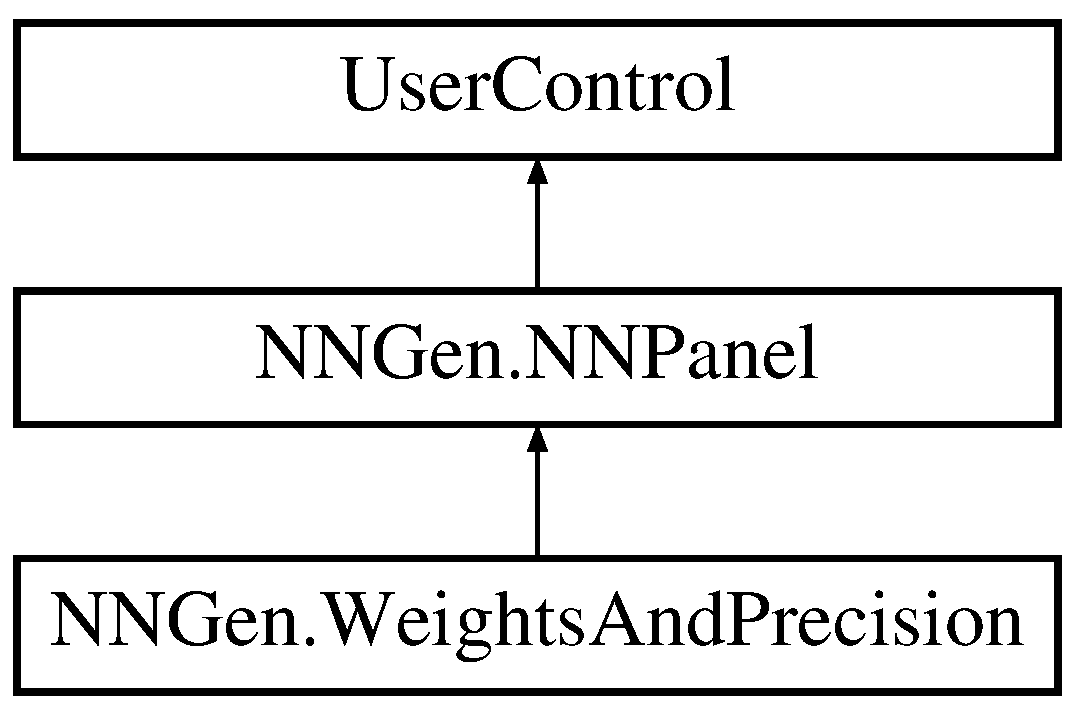
\includegraphics[height=3.000000cm]{class_n_n_gen_1_1_weights_and_precision}
\end{center}
\end{figure}
\subsection*{Public Member Functions}
\begin{DoxyCompactItemize}
\item 
\hyperlink{class_n_n_gen_1_1_weights_and_precision_a16fd27e0739e8a26bbf6f9585e173c7e}{Weights\+And\+Precision} (int \+\_\+num\+Weights\+Expected, int \+\_\+max\+Int\+Bits, int \+\_\+max\+Frac\+Bits, string \+\_\+file\+Path)
\begin{DoxyCompactList}\small\item\em Initialize a \hyperlink{class_n_n_gen_1_1_weights_and_precision}{Weights\+And\+Precision} form \end{DoxyCompactList}\item 
override bool \hyperlink{class_n_n_gen_1_1_weights_and_precision_a55e25affc261256144c0cd9866a63b7a}{verify} ()
\begin{DoxyCompactList}\small\item\em The \hyperlink{class_n_n_gen_1_1_weights_and_precision_a55e25affc261256144c0cd9866a63b7a}{verify()} method implementation for this class. See N\+N\+Pannel.\+verify() for more documentation. \end{DoxyCompactList}\end{DoxyCompactItemize}
\subsection*{Protected Member Functions}
\begin{DoxyCompactItemize}
\item 
override void \hyperlink{class_n_n_gen_1_1_weights_and_precision_af1cc940e6b317254d29e32b7c2ebc70f}{Dispose} (bool disposing)
\begin{DoxyCompactList}\small\item\em Clean up any resources being used. \end{DoxyCompactList}\end{DoxyCompactItemize}
\subsection*{Properties}
\begin{DoxyCompactItemize}
\item 
string \hyperlink{class_n_n_gen_1_1_weights_and_precision_adadd8787371829217f9e9f11fe4f6043}{file\+Path}\hspace{0.3cm}{\ttfamily  \mbox{[}get\mbox{]}}
\begin{DoxyCompactList}\small\item\em The file path from which to load the weights \end{DoxyCompactList}\item 
List$<$ double $>$ \hyperlink{class_n_n_gen_1_1_weights_and_precision_afe90c4fc998ce882228b7bf4459cf100}{weights}\hspace{0.3cm}{\ttfamily  \mbox{[}get\mbox{]}}
\begin{DoxyCompactList}\small\item\em The weights read from the user-\/specified input file \end{DoxyCompactList}\item 
int \hyperlink{class_n_n_gen_1_1_weights_and_precision_a677dd8c72d4d4a7a2b18b292b1a9f6ee}{max\+Int\+Bits}\hspace{0.3cm}{\ttfamily  \mbox{[}get\mbox{]}}
\begin{DoxyCompactList}\small\item\em The number of integer bits to use in the computations \end{DoxyCompactList}\item 
int \hyperlink{class_n_n_gen_1_1_weights_and_precision_a3ee82e53091eb1795bd64cb9b252b952}{max\+Frac\+Bits}\hspace{0.3cm}{\ttfamily  \mbox{[}get\mbox{]}}
\begin{DoxyCompactList}\small\item\em The number of fractional bits to use in the computation \end{DoxyCompactList}\item 
bool \hyperlink{class_n_n_gen_1_1_weights_and_precision_a2dcb1b5045b95f5182ef8e8064931269}{valid\+File\+Selected}\hspace{0.3cm}{\ttfamily  \mbox{[}get\mbox{]}}
\begin{DoxyCompactList}\small\item\em A flag to determine whether a valid file has been selected by the user \end{DoxyCompactList}\item 
int \hyperlink{class_n_n_gen_1_1_weights_and_precision_a670093e800483388eede4a81440dfb0c}{num\+Weights\+Expected}\hspace{0.3cm}{\ttfamily  \mbox{[}get\mbox{]}}
\begin{DoxyCompactList}\small\item\em The number of weights needed to fully initialize the network. \end{DoxyCompactList}\end{DoxyCompactItemize}


\subsection{Detailed Description}
A U\+I element to allow the user to specify the location for the weights to input to the network, as well as the precision with which to perform the neuron\textquotesingle{}s computations. 



\subsection{Constructor \& Destructor Documentation}
\hypertarget{class_n_n_gen_1_1_weights_and_precision_a16fd27e0739e8a26bbf6f9585e173c7e}{}\index{N\+N\+Gen\+::\+Weights\+And\+Precision@{N\+N\+Gen\+::\+Weights\+And\+Precision}!Weights\+And\+Precision@{Weights\+And\+Precision}}
\index{Weights\+And\+Precision@{Weights\+And\+Precision}!N\+N\+Gen\+::\+Weights\+And\+Precision@{N\+N\+Gen\+::\+Weights\+And\+Precision}}
\subsubsection[{Weights\+And\+Precision(int \+\_\+num\+Weights\+Expected, int \+\_\+max\+Int\+Bits, int \+\_\+max\+Frac\+Bits, string \+\_\+file\+Path)}]{\setlength{\rightskip}{0pt plus 5cm}N\+N\+Gen.\+Weights\+And\+Precision.\+Weights\+And\+Precision (
\begin{DoxyParamCaption}
\item[{int}]{\+\_\+num\+Weights\+Expected, }
\item[{int}]{\+\_\+max\+Int\+Bits, }
\item[{int}]{\+\_\+max\+Frac\+Bits, }
\item[{string}]{\+\_\+file\+Path}
\end{DoxyParamCaption}
)\hspace{0.3cm}{\ttfamily [inline]}}\label{class_n_n_gen_1_1_weights_and_precision_a16fd27e0739e8a26bbf6f9585e173c7e}


Initialize a \hyperlink{class_n_n_gen_1_1_weights_and_precision}{Weights\+And\+Precision} form 


\begin{DoxyParams}{Parameters}
{\em \+\_\+num\+Weights\+Expected} & The seed value for the number of weights expected for the network\\
\hline
{\em \+\_\+max\+Int\+Bits} & The seed value for the maximal number of integer bits used in the computation\\
\hline
{\em \+\_\+max\+Frac\+Bits} & The seed value for the maximal number of fractional bits used in the computation\\
\hline
{\em \+\_\+file\+Path} & The seed value for the filepath from which to read the weights\\
\hline
\end{DoxyParams}


\subsection{Member Function Documentation}
\hypertarget{class_n_n_gen_1_1_weights_and_precision_af1cc940e6b317254d29e32b7c2ebc70f}{}\index{N\+N\+Gen\+::\+Weights\+And\+Precision@{N\+N\+Gen\+::\+Weights\+And\+Precision}!Dispose@{Dispose}}
\index{Dispose@{Dispose}!N\+N\+Gen\+::\+Weights\+And\+Precision@{N\+N\+Gen\+::\+Weights\+And\+Precision}}
\subsubsection[{Dispose(bool disposing)}]{\setlength{\rightskip}{0pt plus 5cm}override void N\+N\+Gen.\+Weights\+And\+Precision.\+Dispose (
\begin{DoxyParamCaption}
\item[{bool}]{disposing}
\end{DoxyParamCaption}
)\hspace{0.3cm}{\ttfamily [inline]}, {\ttfamily [protected]}}\label{class_n_n_gen_1_1_weights_and_precision_af1cc940e6b317254d29e32b7c2ebc70f}


Clean up any resources being used. 


\begin{DoxyParams}{Parameters}
{\em disposing} & true if managed resources should be disposed; otherwise, false.\\
\hline
\end{DoxyParams}
\hypertarget{class_n_n_gen_1_1_weights_and_precision_a55e25affc261256144c0cd9866a63b7a}{}\index{N\+N\+Gen\+::\+Weights\+And\+Precision@{N\+N\+Gen\+::\+Weights\+And\+Precision}!verify@{verify}}
\index{verify@{verify}!N\+N\+Gen\+::\+Weights\+And\+Precision@{N\+N\+Gen\+::\+Weights\+And\+Precision}}
\subsubsection[{verify()}]{\setlength{\rightskip}{0pt plus 5cm}override bool N\+N\+Gen.\+Weights\+And\+Precision.\+verify (
\begin{DoxyParamCaption}
{}
\end{DoxyParamCaption}
)\hspace{0.3cm}{\ttfamily [inline]}, {\ttfamily [virtual]}}\label{class_n_n_gen_1_1_weights_and_precision_a55e25affc261256144c0cd9866a63b7a}


The \hyperlink{class_n_n_gen_1_1_weights_and_precision_a55e25affc261256144c0cd9866a63b7a}{verify()} method implementation for this class. See N\+N\+Pannel.\+verify() for more documentation. 

\begin{DoxyReturn}{Returns}

\end{DoxyReturn}


Reimplemented from \hyperlink{class_n_n_gen_1_1_n_n_panel_a36e3bcf90c9e561e8502eac6f884582a}{N\+N\+Gen.\+N\+N\+Panel}.



\subsection{Property Documentation}
\hypertarget{class_n_n_gen_1_1_weights_and_precision_adadd8787371829217f9e9f11fe4f6043}{}\index{N\+N\+Gen\+::\+Weights\+And\+Precision@{N\+N\+Gen\+::\+Weights\+And\+Precision}!file\+Path@{file\+Path}}
\index{file\+Path@{file\+Path}!N\+N\+Gen\+::\+Weights\+And\+Precision@{N\+N\+Gen\+::\+Weights\+And\+Precision}}
\subsubsection[{file\+Path}]{\setlength{\rightskip}{0pt plus 5cm}string N\+N\+Gen.\+Weights\+And\+Precision.\+file\+Path\hspace{0.3cm}{\ttfamily [get]}}\label{class_n_n_gen_1_1_weights_and_precision_adadd8787371829217f9e9f11fe4f6043}


The file path from which to load the weights 

\hypertarget{class_n_n_gen_1_1_weights_and_precision_a3ee82e53091eb1795bd64cb9b252b952}{}\index{N\+N\+Gen\+::\+Weights\+And\+Precision@{N\+N\+Gen\+::\+Weights\+And\+Precision}!max\+Frac\+Bits@{max\+Frac\+Bits}}
\index{max\+Frac\+Bits@{max\+Frac\+Bits}!N\+N\+Gen\+::\+Weights\+And\+Precision@{N\+N\+Gen\+::\+Weights\+And\+Precision}}
\subsubsection[{max\+Frac\+Bits}]{\setlength{\rightskip}{0pt plus 5cm}int N\+N\+Gen.\+Weights\+And\+Precision.\+max\+Frac\+Bits\hspace{0.3cm}{\ttfamily [get]}}\label{class_n_n_gen_1_1_weights_and_precision_a3ee82e53091eb1795bd64cb9b252b952}


The number of fractional bits to use in the computation 

\hypertarget{class_n_n_gen_1_1_weights_and_precision_a677dd8c72d4d4a7a2b18b292b1a9f6ee}{}\index{N\+N\+Gen\+::\+Weights\+And\+Precision@{N\+N\+Gen\+::\+Weights\+And\+Precision}!max\+Int\+Bits@{max\+Int\+Bits}}
\index{max\+Int\+Bits@{max\+Int\+Bits}!N\+N\+Gen\+::\+Weights\+And\+Precision@{N\+N\+Gen\+::\+Weights\+And\+Precision}}
\subsubsection[{max\+Int\+Bits}]{\setlength{\rightskip}{0pt plus 5cm}int N\+N\+Gen.\+Weights\+And\+Precision.\+max\+Int\+Bits\hspace{0.3cm}{\ttfamily [get]}}\label{class_n_n_gen_1_1_weights_and_precision_a677dd8c72d4d4a7a2b18b292b1a9f6ee}


The number of integer bits to use in the computations 

\hypertarget{class_n_n_gen_1_1_weights_and_precision_a670093e800483388eede4a81440dfb0c}{}\index{N\+N\+Gen\+::\+Weights\+And\+Precision@{N\+N\+Gen\+::\+Weights\+And\+Precision}!num\+Weights\+Expected@{num\+Weights\+Expected}}
\index{num\+Weights\+Expected@{num\+Weights\+Expected}!N\+N\+Gen\+::\+Weights\+And\+Precision@{N\+N\+Gen\+::\+Weights\+And\+Precision}}
\subsubsection[{num\+Weights\+Expected}]{\setlength{\rightskip}{0pt plus 5cm}int N\+N\+Gen.\+Weights\+And\+Precision.\+num\+Weights\+Expected\hspace{0.3cm}{\ttfamily [get]}}\label{class_n_n_gen_1_1_weights_and_precision_a670093e800483388eede4a81440dfb0c}


The number of weights needed to fully initialize the network. 

\hypertarget{class_n_n_gen_1_1_weights_and_precision_a2dcb1b5045b95f5182ef8e8064931269}{}\index{N\+N\+Gen\+::\+Weights\+And\+Precision@{N\+N\+Gen\+::\+Weights\+And\+Precision}!valid\+File\+Selected@{valid\+File\+Selected}}
\index{valid\+File\+Selected@{valid\+File\+Selected}!N\+N\+Gen\+::\+Weights\+And\+Precision@{N\+N\+Gen\+::\+Weights\+And\+Precision}}
\subsubsection[{valid\+File\+Selected}]{\setlength{\rightskip}{0pt plus 5cm}bool N\+N\+Gen.\+Weights\+And\+Precision.\+valid\+File\+Selected\hspace{0.3cm}{\ttfamily [get]}}\label{class_n_n_gen_1_1_weights_and_precision_a2dcb1b5045b95f5182ef8e8064931269}


A flag to determine whether a valid file has been selected by the user 

\hypertarget{class_n_n_gen_1_1_weights_and_precision_afe90c4fc998ce882228b7bf4459cf100}{}\index{N\+N\+Gen\+::\+Weights\+And\+Precision@{N\+N\+Gen\+::\+Weights\+And\+Precision}!weights@{weights}}
\index{weights@{weights}!N\+N\+Gen\+::\+Weights\+And\+Precision@{N\+N\+Gen\+::\+Weights\+And\+Precision}}
\subsubsection[{weights}]{\setlength{\rightskip}{0pt plus 5cm}List$<$double$>$ N\+N\+Gen.\+Weights\+And\+Precision.\+weights\hspace{0.3cm}{\ttfamily [get]}}\label{class_n_n_gen_1_1_weights_and_precision_afe90c4fc998ce882228b7bf4459cf100}


The weights read from the user-\/specified input file 



The documentation for this class was generated from the following files\+:\begin{DoxyCompactItemize}
\item 
E\+:/\+Documents/\+Visual Studio 2013/\+Projects/\+Neural\+Network/\+N\+N\+Gen/\hyperlink{_weights_and_precision_8cs}{Weights\+And\+Precision.\+cs}\item 
E\+:/\+Documents/\+Visual Studio 2013/\+Projects/\+Neural\+Network/\+N\+N\+Gen/\hyperlink{_weights_and_precision_8_designer_8cs}{Weights\+And\+Precision.\+Designer.\+cs}\end{DoxyCompactItemize}

\hypertarget{class_n_n_gen_1_1_welcome}{}\section{N\+N\+Gen.\+Welcome Class Reference}
\label{class_n_n_gen_1_1_welcome}\index{N\+N\+Gen.\+Welcome@{N\+N\+Gen.\+Welcome}}


A form displaying the welcome message to the user  


Inheritance diagram for N\+N\+Gen.\+Welcome\+:\begin{figure}[H]
\begin{center}
\leavevmode
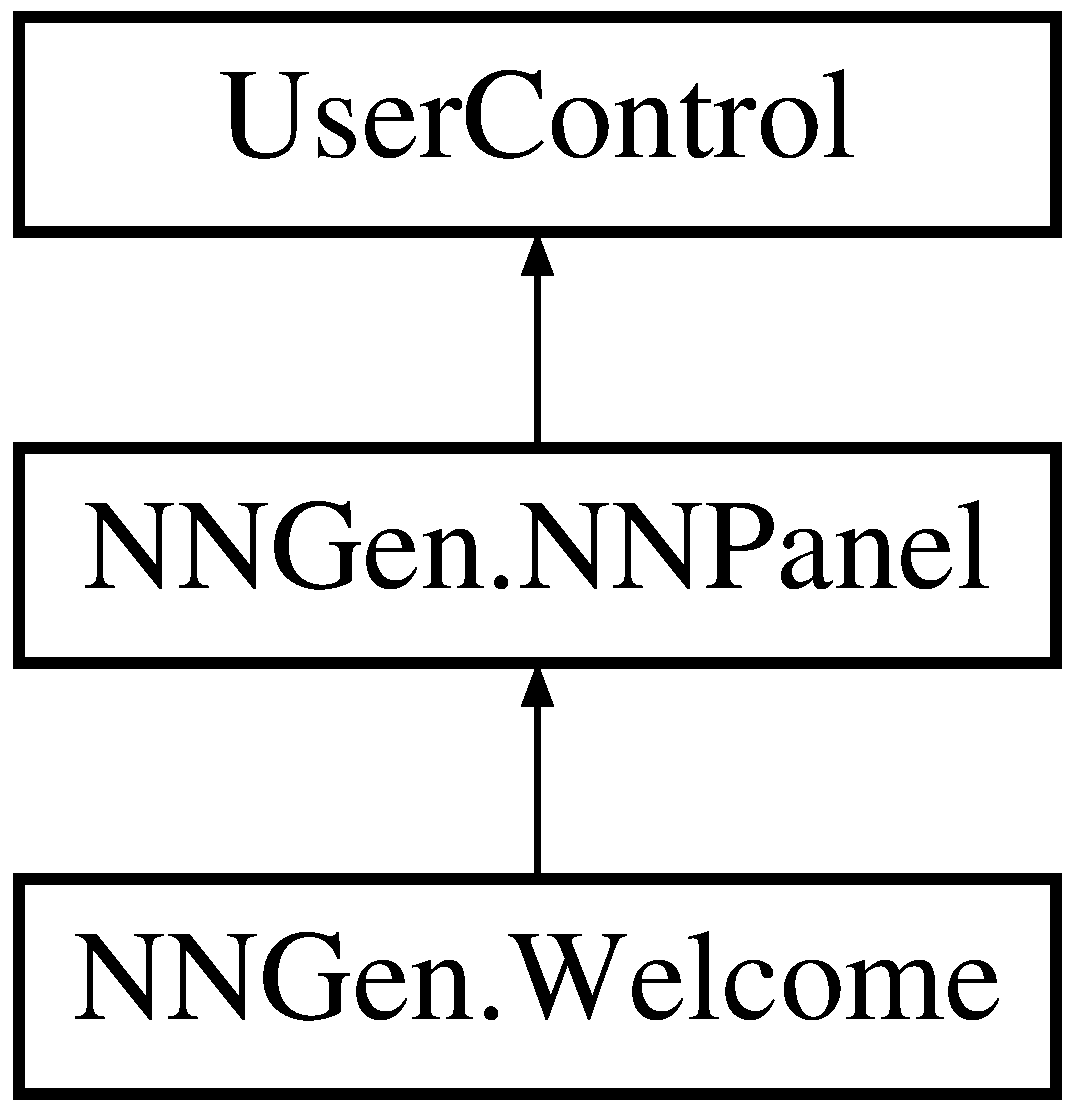
\includegraphics[height=3.000000cm]{class_n_n_gen_1_1_welcome}
\end{center}
\end{figure}
\subsection*{Public Member Functions}
\begin{DoxyCompactItemize}
\item 
\hyperlink{class_n_n_gen_1_1_welcome_aa592b7c0651aada9893adecd6eee5aaf}{Welcome} ()
\begin{DoxyCompactList}\small\item\em Initialize the \hyperlink{class_n_n_gen_1_1_welcome}{Welcome} form \end{DoxyCompactList}\end{DoxyCompactItemize}
\subsection*{Protected Member Functions}
\begin{DoxyCompactItemize}
\item 
override void \hyperlink{class_n_n_gen_1_1_welcome_a28378f009269602807ae9250a2789c13}{Dispose} (bool disposing)
\begin{DoxyCompactList}\small\item\em Clean up any resources being used. \end{DoxyCompactList}\end{DoxyCompactItemize}


\subsection{Detailed Description}
A form displaying the welcome message to the user 



\subsection{Constructor \& Destructor Documentation}
\hypertarget{class_n_n_gen_1_1_welcome_aa592b7c0651aada9893adecd6eee5aaf}{}\index{N\+N\+Gen\+::\+Welcome@{N\+N\+Gen\+::\+Welcome}!Welcome@{Welcome}}
\index{Welcome@{Welcome}!N\+N\+Gen\+::\+Welcome@{N\+N\+Gen\+::\+Welcome}}
\subsubsection[{Welcome()}]{\setlength{\rightskip}{0pt plus 5cm}N\+N\+Gen.\+Welcome.\+Welcome (
\begin{DoxyParamCaption}
{}
\end{DoxyParamCaption}
)\hspace{0.3cm}{\ttfamily [inline]}}\label{class_n_n_gen_1_1_welcome_aa592b7c0651aada9893adecd6eee5aaf}


Initialize the \hyperlink{class_n_n_gen_1_1_welcome}{Welcome} form 



\subsection{Member Function Documentation}
\hypertarget{class_n_n_gen_1_1_welcome_a28378f009269602807ae9250a2789c13}{}\index{N\+N\+Gen\+::\+Welcome@{N\+N\+Gen\+::\+Welcome}!Dispose@{Dispose}}
\index{Dispose@{Dispose}!N\+N\+Gen\+::\+Welcome@{N\+N\+Gen\+::\+Welcome}}
\subsubsection[{Dispose(bool disposing)}]{\setlength{\rightskip}{0pt plus 5cm}override void N\+N\+Gen.\+Welcome.\+Dispose (
\begin{DoxyParamCaption}
\item[{bool}]{disposing}
\end{DoxyParamCaption}
)\hspace{0.3cm}{\ttfamily [inline]}, {\ttfamily [protected]}}\label{class_n_n_gen_1_1_welcome_a28378f009269602807ae9250a2789c13}


Clean up any resources being used. 


\begin{DoxyParams}{Parameters}
{\em disposing} & true if managed resources should be disposed; otherwise, false.\\
\hline
\end{DoxyParams}


The documentation for this class was generated from the following files\+:\begin{DoxyCompactItemize}
\item 
E\+:/\+Documents/\+Visual Studio 2013/\+Projects/\+Neural\+Network/\+N\+N\+Gen/\hyperlink{_welcome_8cs}{Welcome.\+cs}\item 
E\+:/\+Documents/\+Visual Studio 2013/\+Projects/\+Neural\+Network/\+N\+N\+Gen/\hyperlink{_welcome_8_designer_8cs}{Welcome.\+Designer.\+cs}\end{DoxyCompactItemize}

\hypertarget{class_n_n_gen_1_1_wizard_controller}{}\section{N\+N\+Gen.\+Wizard\+Controller Class Reference}
\label{class_n_n_gen_1_1_wizard_controller}\index{N\+N\+Gen.\+Wizard\+Controller@{N\+N\+Gen.\+Wizard\+Controller}}


A class managing the U\+I forms to show the user, as well as recording their responses  


\subsection*{Public Member Functions}
\begin{DoxyCompactItemize}
\item 
\hyperlink{class_n_n_gen_1_1_wizard_controller_ab4b572ad55d5e544cc65cbf850e4bcf8}{Wizard\+Controller} ()
\begin{DoxyCompactList}\small\item\em Create a new wizard controller \end{DoxyCompactList}\item 
\hyperlink{class_n_n_gen_1_1_n_n_panel}{N\+N\+Panel} \hyperlink{class_n_n_gen_1_1_wizard_controller_a8cb8ef289bd566a55e9cf63448fb503f}{next} (int width, int height)
\begin{DoxyCompactList}\small\item\em Get the next screen to show the user \end{DoxyCompactList}\item 
\hyperlink{class_n_n_gen_1_1_n_n_panel}{N\+N\+Panel} \hyperlink{class_n_n_gen_1_1_wizard_controller_a56f2cde3be2146a4d215bae7cc773b42}{previous} (int width, int height)
\begin{DoxyCompactList}\small\item\em Get the previous screen to display to the user \end{DoxyCompactList}\item 
\hyperlink{class_n_n_gen_1_1_n_n_panel}{N\+N\+Panel} \hyperlink{class_n_n_gen_1_1_wizard_controller_a7fad78197da21bbd70fbd874d16712cb}{current} (int width, int height)
\begin{DoxyCompactList}\small\item\em Get the current screen \end{DoxyCompactList}\item 
bool \hyperlink{class_n_n_gen_1_1_wizard_controller_abdc2fb0f10dc7fc8fd0fec5f048060f4}{generate\+N\+N} (string filepath)
\begin{DoxyCompactList}\small\item\em Writes the neural network files to disk \end{DoxyCompactList}\end{DoxyCompactItemize}
\subsection*{Properties}
\begin{DoxyCompactItemize}
\item 
\hyperlink{class_n_n_gen_1_1_panel_container}{Panel\+Container} \hyperlink{class_n_n_gen_1_1_wizard_controller_a9954efe53bf629492e68dd6692092a94}{pc}\hspace{0.3cm}{\ttfamily  \mbox{[}get\mbox{]}}
\begin{DoxyCompactList}\small\item\em The container for the panels to show the user \end{DoxyCompactList}\item 
int\mbox{[}$\,$\mbox{]} \hyperlink{class_n_n_gen_1_1_wizard_controller_ad5eb425198c744f28f5e228eeffc895b}{neuron\+Counts}\hspace{0.3cm}{\ttfamily  \mbox{[}get\mbox{]}}
\begin{DoxyCompactList}\small\item\em An array holding the number of neurons for the network. The i-\/th row represents the i-\/th layer \end{DoxyCompactList}\item 
double\mbox{[}$\,$\mbox{]} \hyperlink{class_n_n_gen_1_1_wizard_controller_a0575bbc3820b30e2890579150cb924f0}{bias\+Values}\hspace{0.3cm}{\ttfamily  \mbox{[}get\mbox{]}}
\begin{DoxyCompactList}\small\item\em An array holding the bias values for the networks. The i-\/th row represents the bias value feeding into the i+1-\/th layer \end{DoxyCompactList}\item 
\hyperlink{class_n_n_gen_1_1_async_neuron_afe8460a52808d1587cbcc0a8e4e23b64}{Async\+Neuron.\+Neuron\+Activation\+Type}\mbox{[}$\,$\mbox{]} \hyperlink{class_n_n_gen_1_1_wizard_controller_acbc7dd16f2727da7272632e3737989d6}{async\+Activation\+Types}\hspace{0.3cm}{\ttfamily  \mbox{[}get\mbox{]}}
\begin{DoxyCompactList}\small\item\em For asynchronous networks, the activation type of each layer. For synchronous networks, this variable is ignored \end{DoxyCompactList}\item 
\hyperlink{class_n_n_gen_1_1_transfer_function_wrapper_aa338ffadb8fcdf76df75419374a51ff6}{Transfer\+Function\+Wrapper.\+Memory\+Activation\+Type}\mbox{[}$\,$\mbox{]} \hyperlink{class_n_n_gen_1_1_wizard_controller_ad211fa93c8e54fb2f0383889bcb28964}{sync\+Activation\+Types}\hspace{0.3cm}{\ttfamily  \mbox{[}get\mbox{]}}
\begin{DoxyCompactList}\small\item\em For synchronous networks, the activation types of each layer. For asynchronous netowrks, this variable is ignored \end{DoxyCompactList}\item 
int \hyperlink{class_n_n_gen_1_1_wizard_controller_a5216441fbf991464e4db1b1cc1d54c2d}{num\+Int\+Bits}\hspace{0.3cm}{\ttfamily  \mbox{[}get\mbox{]}}
\begin{DoxyCompactList}\small\item\em The number of integer bits to use in the creation of the neurons \end{DoxyCompactList}\item 
int \hyperlink{class_n_n_gen_1_1_wizard_controller_a49f443f5a43ad1afbbf72a4176e1dcd6}{num\+Frac\+Bits}\hspace{0.3cm}{\ttfamily  \mbox{[}get\mbox{]}}
\begin{DoxyCompactList}\small\item\em The number of fractional bits to use in the creation of the neurons \end{DoxyCompactList}\item 
int \hyperlink{class_n_n_gen_1_1_wizard_controller_a8aafaab7cca2632ebd09f0fba6a2f09a}{num\+Weight\+Int\+Bits}\hspace{0.3cm}{\ttfamily  \mbox{[}get\mbox{]}}
\begin{DoxyCompactList}\small\item\em Then number of integer bits to use in the creation of the weight memory \end{DoxyCompactList}\item 
bool \hyperlink{class_n_n_gen_1_1_wizard_controller_a9314043770a6c63e71dadc2c3abaf63a}{is\+Classifier}\hspace{0.3cm}{\ttfamily  \mbox{[}get\mbox{]}}
\begin{DoxyCompactList}\small\item\em A flag to save whether the network is a classification network or not. \end{DoxyCompactList}\item 
bool \hyperlink{class_n_n_gen_1_1_wizard_controller_aa3186397159e779da8e2007b9f1c2884}{is\+Synchronous\+Network}\hspace{0.3cm}{\ttfamily  \mbox{[}get\mbox{]}}
\begin{DoxyCompactList}\small\item\em A flag to represent whether the network being created is synchronous or not \end{DoxyCompactList}\item 
double\mbox{[}$\,$\mbox{]} \hyperlink{class_n_n_gen_1_1_wizard_controller_a77607ae6650b0c79f9b503209badce0f}{classifier\+Thresholds}\hspace{0.3cm}{\ttfamily  \mbox{[}get\mbox{]}}
\begin{DoxyCompactList}\small\item\em The classifier thresholds for a classification network. For a regression network, these are null. \end{DoxyCompactList}\item 
List$<$ double $>$ \hyperlink{class_n_n_gen_1_1_wizard_controller_a6978f46ec504d8be14ec6517959d131a}{weights}\hspace{0.3cm}{\ttfamily  \mbox{[}get\mbox{]}}
\begin{DoxyCompactList}\small\item\em The list of neuron input weights \end{DoxyCompactList}\item 
\hyperlink{class_n_n_gen_1_1_async_neural_network}{Async\+Neural\+Network} \hyperlink{class_n_n_gen_1_1_wizard_controller_a5bc403949233d912bb2c93e2f43cbc25}{async\+N\+N}\hspace{0.3cm}{\ttfamily  \mbox{[}get\mbox{]}}
\begin{DoxyCompactList}\small\item\em The asynchronous network object to be created. This variable is ignored for synchronous networks \end{DoxyCompactList}\item 
\hyperlink{class_n_n_gen_1_1_sync_neural_network}{Sync\+Neural\+Network} \hyperlink{class_n_n_gen_1_1_wizard_controller_a6231cf0c8041896d72a7225cc5cdef7f}{sync\+N\+N}\hspace{0.3cm}{\ttfamily  \mbox{[}get\mbox{]}}
\begin{DoxyCompactList}\small\item\em The synchronous network object to be created. This variable is ignored for asynchronous networks \end{DoxyCompactList}\end{DoxyCompactItemize}


\subsection{Detailed Description}
A class managing the U\+I forms to show the user, as well as recording their responses 



\subsection{Constructor \& Destructor Documentation}
\hypertarget{class_n_n_gen_1_1_wizard_controller_ab4b572ad55d5e544cc65cbf850e4bcf8}{}\index{N\+N\+Gen\+::\+Wizard\+Controller@{N\+N\+Gen\+::\+Wizard\+Controller}!Wizard\+Controller@{Wizard\+Controller}}
\index{Wizard\+Controller@{Wizard\+Controller}!N\+N\+Gen\+::\+Wizard\+Controller@{N\+N\+Gen\+::\+Wizard\+Controller}}
\subsubsection[{Wizard\+Controller()}]{\setlength{\rightskip}{0pt plus 5cm}N\+N\+Gen.\+Wizard\+Controller.\+Wizard\+Controller (
\begin{DoxyParamCaption}
{}
\end{DoxyParamCaption}
)\hspace{0.3cm}{\ttfamily [inline]}}\label{class_n_n_gen_1_1_wizard_controller_ab4b572ad55d5e544cc65cbf850e4bcf8}


Create a new wizard controller 



\subsection{Member Function Documentation}
\hypertarget{class_n_n_gen_1_1_wizard_controller_a7fad78197da21bbd70fbd874d16712cb}{}\index{N\+N\+Gen\+::\+Wizard\+Controller@{N\+N\+Gen\+::\+Wizard\+Controller}!current@{current}}
\index{current@{current}!N\+N\+Gen\+::\+Wizard\+Controller@{N\+N\+Gen\+::\+Wizard\+Controller}}
\subsubsection[{current(int width, int height)}]{\setlength{\rightskip}{0pt plus 5cm}{\bf N\+N\+Panel} N\+N\+Gen.\+Wizard\+Controller.\+current (
\begin{DoxyParamCaption}
\item[{int}]{width, }
\item[{int}]{height}
\end{DoxyParamCaption}
)\hspace{0.3cm}{\ttfamily [inline]}}\label{class_n_n_gen_1_1_wizard_controller_a7fad78197da21bbd70fbd874d16712cb}


Get the current screen 


\begin{DoxyParams}{Parameters}
{\em width} & The width at which to display the screen\\
\hline
{\em height} & The height at which to display the screen\\
\hline
\end{DoxyParams}
\begin{DoxyReturn}{Returns}

\end{DoxyReturn}
\hypertarget{class_n_n_gen_1_1_wizard_controller_abdc2fb0f10dc7fc8fd0fec5f048060f4}{}\index{N\+N\+Gen\+::\+Wizard\+Controller@{N\+N\+Gen\+::\+Wizard\+Controller}!generate\+N\+N@{generate\+N\+N}}
\index{generate\+N\+N@{generate\+N\+N}!N\+N\+Gen\+::\+Wizard\+Controller@{N\+N\+Gen\+::\+Wizard\+Controller}}
\subsubsection[{generate\+N\+N(string filepath)}]{\setlength{\rightskip}{0pt plus 5cm}bool N\+N\+Gen.\+Wizard\+Controller.\+generate\+N\+N (
\begin{DoxyParamCaption}
\item[{string}]{filepath}
\end{DoxyParamCaption}
)\hspace{0.3cm}{\ttfamily [inline]}}\label{class_n_n_gen_1_1_wizard_controller_abdc2fb0f10dc7fc8fd0fec5f048060f4}


Writes the neural network files to disk 


\begin{DoxyParams}{Parameters}
{\em filepath} & The path at which to write the data\\
\hline
\end{DoxyParams}
\begin{DoxyReturn}{Returns}

\end{DoxyReturn}
\hypertarget{class_n_n_gen_1_1_wizard_controller_a8cb8ef289bd566a55e9cf63448fb503f}{}\index{N\+N\+Gen\+::\+Wizard\+Controller@{N\+N\+Gen\+::\+Wizard\+Controller}!next@{next}}
\index{next@{next}!N\+N\+Gen\+::\+Wizard\+Controller@{N\+N\+Gen\+::\+Wizard\+Controller}}
\subsubsection[{next(int width, int height)}]{\setlength{\rightskip}{0pt plus 5cm}{\bf N\+N\+Panel} N\+N\+Gen.\+Wizard\+Controller.\+next (
\begin{DoxyParamCaption}
\item[{int}]{width, }
\item[{int}]{height}
\end{DoxyParamCaption}
)\hspace{0.3cm}{\ttfamily [inline]}}\label{class_n_n_gen_1_1_wizard_controller_a8cb8ef289bd566a55e9cf63448fb503f}


Get the next screen to show the user 


\begin{DoxyParams}{Parameters}
{\em width} & The width at which to display the form\\
\hline
{\em height} & The height at which to display the form\\
\hline
\end{DoxyParams}
\begin{DoxyReturn}{Returns}

\end{DoxyReturn}
\hypertarget{class_n_n_gen_1_1_wizard_controller_a56f2cde3be2146a4d215bae7cc773b42}{}\index{N\+N\+Gen\+::\+Wizard\+Controller@{N\+N\+Gen\+::\+Wizard\+Controller}!previous@{previous}}
\index{previous@{previous}!N\+N\+Gen\+::\+Wizard\+Controller@{N\+N\+Gen\+::\+Wizard\+Controller}}
\subsubsection[{previous(int width, int height)}]{\setlength{\rightskip}{0pt plus 5cm}{\bf N\+N\+Panel} N\+N\+Gen.\+Wizard\+Controller.\+previous (
\begin{DoxyParamCaption}
\item[{int}]{width, }
\item[{int}]{height}
\end{DoxyParamCaption}
)\hspace{0.3cm}{\ttfamily [inline]}}\label{class_n_n_gen_1_1_wizard_controller_a56f2cde3be2146a4d215bae7cc773b42}


Get the previous screen to display to the user 


\begin{DoxyParams}{Parameters}
{\em width} & The width at which to display the screen\\
\hline
{\em height} & The height at which to display the screen\\
\hline
\end{DoxyParams}
\begin{DoxyReturn}{Returns}

\end{DoxyReturn}


\subsection{Property Documentation}
\hypertarget{class_n_n_gen_1_1_wizard_controller_acbc7dd16f2727da7272632e3737989d6}{}\index{N\+N\+Gen\+::\+Wizard\+Controller@{N\+N\+Gen\+::\+Wizard\+Controller}!async\+Activation\+Types@{async\+Activation\+Types}}
\index{async\+Activation\+Types@{async\+Activation\+Types}!N\+N\+Gen\+::\+Wizard\+Controller@{N\+N\+Gen\+::\+Wizard\+Controller}}
\subsubsection[{async\+Activation\+Types}]{\setlength{\rightskip}{0pt plus 5cm}{\bf Async\+Neuron.\+Neuron\+Activation\+Type} \mbox{[}$\,$\mbox{]} N\+N\+Gen.\+Wizard\+Controller.\+async\+Activation\+Types\hspace{0.3cm}{\ttfamily [get]}}\label{class_n_n_gen_1_1_wizard_controller_acbc7dd16f2727da7272632e3737989d6}


For asynchronous networks, the activation type of each layer. For synchronous networks, this variable is ignored 

\hypertarget{class_n_n_gen_1_1_wizard_controller_a5bc403949233d912bb2c93e2f43cbc25}{}\index{N\+N\+Gen\+::\+Wizard\+Controller@{N\+N\+Gen\+::\+Wizard\+Controller}!async\+N\+N@{async\+N\+N}}
\index{async\+N\+N@{async\+N\+N}!N\+N\+Gen\+::\+Wizard\+Controller@{N\+N\+Gen\+::\+Wizard\+Controller}}
\subsubsection[{async\+N\+N}]{\setlength{\rightskip}{0pt plus 5cm}{\bf Async\+Neural\+Network} N\+N\+Gen.\+Wizard\+Controller.\+async\+N\+N\hspace{0.3cm}{\ttfamily [get]}}\label{class_n_n_gen_1_1_wizard_controller_a5bc403949233d912bb2c93e2f43cbc25}


The asynchronous network object to be created. This variable is ignored for synchronous networks 

\hypertarget{class_n_n_gen_1_1_wizard_controller_a0575bbc3820b30e2890579150cb924f0}{}\index{N\+N\+Gen\+::\+Wizard\+Controller@{N\+N\+Gen\+::\+Wizard\+Controller}!bias\+Values@{bias\+Values}}
\index{bias\+Values@{bias\+Values}!N\+N\+Gen\+::\+Wizard\+Controller@{N\+N\+Gen\+::\+Wizard\+Controller}}
\subsubsection[{bias\+Values}]{\setlength{\rightskip}{0pt plus 5cm}double \mbox{[}$\,$\mbox{]} N\+N\+Gen.\+Wizard\+Controller.\+bias\+Values\hspace{0.3cm}{\ttfamily [get]}}\label{class_n_n_gen_1_1_wizard_controller_a0575bbc3820b30e2890579150cb924f0}


An array holding the bias values for the networks. The i-\/th row represents the bias value feeding into the i+1-\/th layer 

\hypertarget{class_n_n_gen_1_1_wizard_controller_a77607ae6650b0c79f9b503209badce0f}{}\index{N\+N\+Gen\+::\+Wizard\+Controller@{N\+N\+Gen\+::\+Wizard\+Controller}!classifier\+Thresholds@{classifier\+Thresholds}}
\index{classifier\+Thresholds@{classifier\+Thresholds}!N\+N\+Gen\+::\+Wizard\+Controller@{N\+N\+Gen\+::\+Wizard\+Controller}}
\subsubsection[{classifier\+Thresholds}]{\setlength{\rightskip}{0pt plus 5cm}double \mbox{[}$\,$\mbox{]} N\+N\+Gen.\+Wizard\+Controller.\+classifier\+Thresholds\hspace{0.3cm}{\ttfamily [get]}}\label{class_n_n_gen_1_1_wizard_controller_a77607ae6650b0c79f9b503209badce0f}


The classifier thresholds for a classification network. For a regression network, these are null. 

\hypertarget{class_n_n_gen_1_1_wizard_controller_a9314043770a6c63e71dadc2c3abaf63a}{}\index{N\+N\+Gen\+::\+Wizard\+Controller@{N\+N\+Gen\+::\+Wizard\+Controller}!is\+Classifier@{is\+Classifier}}
\index{is\+Classifier@{is\+Classifier}!N\+N\+Gen\+::\+Wizard\+Controller@{N\+N\+Gen\+::\+Wizard\+Controller}}
\subsubsection[{is\+Classifier}]{\setlength{\rightskip}{0pt plus 5cm}bool N\+N\+Gen.\+Wizard\+Controller.\+is\+Classifier\hspace{0.3cm}{\ttfamily [get]}}\label{class_n_n_gen_1_1_wizard_controller_a9314043770a6c63e71dadc2c3abaf63a}


A flag to save whether the network is a classification network or not. 

\hypertarget{class_n_n_gen_1_1_wizard_controller_aa3186397159e779da8e2007b9f1c2884}{}\index{N\+N\+Gen\+::\+Wizard\+Controller@{N\+N\+Gen\+::\+Wizard\+Controller}!is\+Synchronous\+Network@{is\+Synchronous\+Network}}
\index{is\+Synchronous\+Network@{is\+Synchronous\+Network}!N\+N\+Gen\+::\+Wizard\+Controller@{N\+N\+Gen\+::\+Wizard\+Controller}}
\subsubsection[{is\+Synchronous\+Network}]{\setlength{\rightskip}{0pt plus 5cm}bool N\+N\+Gen.\+Wizard\+Controller.\+is\+Synchronous\+Network\hspace{0.3cm}{\ttfamily [get]}}\label{class_n_n_gen_1_1_wizard_controller_aa3186397159e779da8e2007b9f1c2884}


A flag to represent whether the network being created is synchronous or not 

\hypertarget{class_n_n_gen_1_1_wizard_controller_ad5eb425198c744f28f5e228eeffc895b}{}\index{N\+N\+Gen\+::\+Wizard\+Controller@{N\+N\+Gen\+::\+Wizard\+Controller}!neuron\+Counts@{neuron\+Counts}}
\index{neuron\+Counts@{neuron\+Counts}!N\+N\+Gen\+::\+Wizard\+Controller@{N\+N\+Gen\+::\+Wizard\+Controller}}
\subsubsection[{neuron\+Counts}]{\setlength{\rightskip}{0pt plus 5cm}int \mbox{[}$\,$\mbox{]} N\+N\+Gen.\+Wizard\+Controller.\+neuron\+Counts\hspace{0.3cm}{\ttfamily [get]}}\label{class_n_n_gen_1_1_wizard_controller_ad5eb425198c744f28f5e228eeffc895b}


An array holding the number of neurons for the network. The i-\/th row represents the i-\/th layer 

\hypertarget{class_n_n_gen_1_1_wizard_controller_a49f443f5a43ad1afbbf72a4176e1dcd6}{}\index{N\+N\+Gen\+::\+Wizard\+Controller@{N\+N\+Gen\+::\+Wizard\+Controller}!num\+Frac\+Bits@{num\+Frac\+Bits}}
\index{num\+Frac\+Bits@{num\+Frac\+Bits}!N\+N\+Gen\+::\+Wizard\+Controller@{N\+N\+Gen\+::\+Wizard\+Controller}}
\subsubsection[{num\+Frac\+Bits}]{\setlength{\rightskip}{0pt plus 5cm}int N\+N\+Gen.\+Wizard\+Controller.\+num\+Frac\+Bits\hspace{0.3cm}{\ttfamily [get]}}\label{class_n_n_gen_1_1_wizard_controller_a49f443f5a43ad1afbbf72a4176e1dcd6}


The number of fractional bits to use in the creation of the neurons 

\hypertarget{class_n_n_gen_1_1_wizard_controller_a5216441fbf991464e4db1b1cc1d54c2d}{}\index{N\+N\+Gen\+::\+Wizard\+Controller@{N\+N\+Gen\+::\+Wizard\+Controller}!num\+Int\+Bits@{num\+Int\+Bits}}
\index{num\+Int\+Bits@{num\+Int\+Bits}!N\+N\+Gen\+::\+Wizard\+Controller@{N\+N\+Gen\+::\+Wizard\+Controller}}
\subsubsection[{num\+Int\+Bits}]{\setlength{\rightskip}{0pt plus 5cm}int N\+N\+Gen.\+Wizard\+Controller.\+num\+Int\+Bits\hspace{0.3cm}{\ttfamily [get]}}\label{class_n_n_gen_1_1_wizard_controller_a5216441fbf991464e4db1b1cc1d54c2d}


The number of integer bits to use in the creation of the neurons 

\hypertarget{class_n_n_gen_1_1_wizard_controller_a8aafaab7cca2632ebd09f0fba6a2f09a}{}\index{N\+N\+Gen\+::\+Wizard\+Controller@{N\+N\+Gen\+::\+Wizard\+Controller}!num\+Weight\+Int\+Bits@{num\+Weight\+Int\+Bits}}
\index{num\+Weight\+Int\+Bits@{num\+Weight\+Int\+Bits}!N\+N\+Gen\+::\+Wizard\+Controller@{N\+N\+Gen\+::\+Wizard\+Controller}}
\subsubsection[{num\+Weight\+Int\+Bits}]{\setlength{\rightskip}{0pt plus 5cm}int N\+N\+Gen.\+Wizard\+Controller.\+num\+Weight\+Int\+Bits\hspace{0.3cm}{\ttfamily [get]}}\label{class_n_n_gen_1_1_wizard_controller_a8aafaab7cca2632ebd09f0fba6a2f09a}


Then number of integer bits to use in the creation of the weight memory 

\hypertarget{class_n_n_gen_1_1_wizard_controller_a9954efe53bf629492e68dd6692092a94}{}\index{N\+N\+Gen\+::\+Wizard\+Controller@{N\+N\+Gen\+::\+Wizard\+Controller}!pc@{pc}}
\index{pc@{pc}!N\+N\+Gen\+::\+Wizard\+Controller@{N\+N\+Gen\+::\+Wizard\+Controller}}
\subsubsection[{pc}]{\setlength{\rightskip}{0pt plus 5cm}{\bf Panel\+Container} N\+N\+Gen.\+Wizard\+Controller.\+pc\hspace{0.3cm}{\ttfamily [get]}}\label{class_n_n_gen_1_1_wizard_controller_a9954efe53bf629492e68dd6692092a94}


The container for the panels to show the user 

\hypertarget{class_n_n_gen_1_1_wizard_controller_ad211fa93c8e54fb2f0383889bcb28964}{}\index{N\+N\+Gen\+::\+Wizard\+Controller@{N\+N\+Gen\+::\+Wizard\+Controller}!sync\+Activation\+Types@{sync\+Activation\+Types}}
\index{sync\+Activation\+Types@{sync\+Activation\+Types}!N\+N\+Gen\+::\+Wizard\+Controller@{N\+N\+Gen\+::\+Wizard\+Controller}}
\subsubsection[{sync\+Activation\+Types}]{\setlength{\rightskip}{0pt plus 5cm}{\bf Transfer\+Function\+Wrapper.\+Memory\+Activation\+Type} \mbox{[}$\,$\mbox{]} N\+N\+Gen.\+Wizard\+Controller.\+sync\+Activation\+Types\hspace{0.3cm}{\ttfamily [get]}}\label{class_n_n_gen_1_1_wizard_controller_ad211fa93c8e54fb2f0383889bcb28964}


For synchronous networks, the activation types of each layer. For asynchronous netowrks, this variable is ignored 

\hypertarget{class_n_n_gen_1_1_wizard_controller_a6231cf0c8041896d72a7225cc5cdef7f}{}\index{N\+N\+Gen\+::\+Wizard\+Controller@{N\+N\+Gen\+::\+Wizard\+Controller}!sync\+N\+N@{sync\+N\+N}}
\index{sync\+N\+N@{sync\+N\+N}!N\+N\+Gen\+::\+Wizard\+Controller@{N\+N\+Gen\+::\+Wizard\+Controller}}
\subsubsection[{sync\+N\+N}]{\setlength{\rightskip}{0pt plus 5cm}{\bf Sync\+Neural\+Network} N\+N\+Gen.\+Wizard\+Controller.\+sync\+N\+N\hspace{0.3cm}{\ttfamily [get]}}\label{class_n_n_gen_1_1_wizard_controller_a6231cf0c8041896d72a7225cc5cdef7f}


The synchronous network object to be created. This variable is ignored for asynchronous networks 

\hypertarget{class_n_n_gen_1_1_wizard_controller_a6978f46ec504d8be14ec6517959d131a}{}\index{N\+N\+Gen\+::\+Wizard\+Controller@{N\+N\+Gen\+::\+Wizard\+Controller}!weights@{weights}}
\index{weights@{weights}!N\+N\+Gen\+::\+Wizard\+Controller@{N\+N\+Gen\+::\+Wizard\+Controller}}
\subsubsection[{weights}]{\setlength{\rightskip}{0pt plus 5cm}List$<$double$>$ N\+N\+Gen.\+Wizard\+Controller.\+weights\hspace{0.3cm}{\ttfamily [get]}}\label{class_n_n_gen_1_1_wizard_controller_a6978f46ec504d8be14ec6517959d131a}


The list of neuron input weights 



The documentation for this class was generated from the following file\+:\begin{DoxyCompactItemize}
\item 
E\+:/\+Documents/\+Visual Studio 2013/\+Projects/\+Neural\+Network/\+N\+N\+Gen/\hyperlink{_wizard_controller_8cs}{Wizard\+Controller.\+cs}\end{DoxyCompactItemize}

\chapter{File Documentation}
\hypertarget{_array_signal_8cs}{}\section{E\+:/\+Documents/\+Visual Studio 2013/\+Projects/\+Neural\+Network/\+N\+N\+Gen/\+Array\+Signal.cs File Reference}
\label{_array_signal_8cs}\index{E\+:/\+Documents/\+Visual Studio 2013/\+Projects/\+Neural\+Network/\+N\+N\+Gen/\+Array\+Signal.\+cs@{E\+:/\+Documents/\+Visual Studio 2013/\+Projects/\+Neural\+Network/\+N\+N\+Gen/\+Array\+Signal.\+cs}}
\subsection*{Classes}
\begin{DoxyCompactItemize}
\item 
class \hyperlink{class_n_n_gen_1_1_array_signal}{N\+N\+Gen.\+Array\+Signal}
\begin{DoxyCompactList}\small\item\em A class to represent an array of signals \end{DoxyCompactList}\end{DoxyCompactItemize}
\subsection*{Namespaces}
\begin{DoxyCompactItemize}
\item 
namespace \hyperlink{namespace_n_n_gen}{N\+N\+Gen}
\end{DoxyCompactItemize}

\hypertarget{_async_neural_network_8cs}{}\section{E\+:/\+Documents/\+Visual Studio 2013/\+Projects/\+Neural\+Network/\+N\+N\+Gen/\+Async\+Neural\+Network.cs File Reference}
\label{_async_neural_network_8cs}\index{E\+:/\+Documents/\+Visual Studio 2013/\+Projects/\+Neural\+Network/\+N\+N\+Gen/\+Async\+Neural\+Network.\+cs@{E\+:/\+Documents/\+Visual Studio 2013/\+Projects/\+Neural\+Network/\+N\+N\+Gen/\+Async\+Neural\+Network.\+cs}}
\subsection*{Classes}
\begin{DoxyCompactItemize}
\item 
class \hyperlink{class_n_n_gen_1_1_async_neural_network}{N\+N\+Gen.\+Async\+Neural\+Network}
\begin{DoxyCompactList}\small\item\em An abstraction of a neural network entity. \end{DoxyCompactList}\end{DoxyCompactItemize}
\subsection*{Namespaces}
\begin{DoxyCompactItemize}
\item 
namespace \hyperlink{namespace_n_n_gen}{N\+N\+Gen}
\end{DoxyCompactItemize}

\hypertarget{_async_neuron_8cs}{}\section{E\+:/\+Documents/\+Visual Studio 2013/\+Projects/\+Neural\+Network/\+N\+N\+Gen/\+Async\+Neuron.cs File Reference}
\label{_async_neuron_8cs}\index{E\+:/\+Documents/\+Visual Studio 2013/\+Projects/\+Neural\+Network/\+N\+N\+Gen/\+Async\+Neuron.\+cs@{E\+:/\+Documents/\+Visual Studio 2013/\+Projects/\+Neural\+Network/\+N\+N\+Gen/\+Async\+Neuron.\+cs}}
\subsection*{Classes}
\begin{DoxyCompactItemize}
\item 
class \hyperlink{class_n_n_gen_1_1_async_neuron}{N\+N\+Gen.\+Async\+Neuron}
\begin{DoxyCompactList}\small\item\em An abstraction of a single neuron within a network \end{DoxyCompactList}\end{DoxyCompactItemize}
\subsection*{Namespaces}
\begin{DoxyCompactItemize}
\item 
namespace \hyperlink{namespace_n_n_gen}{N\+N\+Gen}
\end{DoxyCompactItemize}

\hypertarget{_entity_8cs}{}\section{E\+:/\+Documents/\+Visual Studio 2013/\+Projects/\+Neural\+Network/\+N\+N\+Gen/\+Entity.cs File Reference}
\label{_entity_8cs}\index{E\+:/\+Documents/\+Visual Studio 2013/\+Projects/\+Neural\+Network/\+N\+N\+Gen/\+Entity.\+cs@{E\+:/\+Documents/\+Visual Studio 2013/\+Projects/\+Neural\+Network/\+N\+N\+Gen/\+Entity.\+cs}}
\subsection*{Classes}
\begin{DoxyCompactItemize}
\item 
class \hyperlink{class_n_n_gen_1_1_entity}{N\+N\+Gen.\+Entity}
\begin{DoxyCompactList}\small\item\em An interface for any object that will eventually generate a V\+H\+D\+L entity \end{DoxyCompactList}\end{DoxyCompactItemize}
\subsection*{Namespaces}
\begin{DoxyCompactItemize}
\item 
namespace \hyperlink{namespace_n_n_gen}{N\+N\+Gen}
\end{DoxyCompactItemize}

\hypertarget{_form1_8cs}{}\section{E\+:/\+Documents/\+Visual Studio 2013/\+Projects/\+Neural\+Network/\+N\+N\+Gen/\+Form1.cs File Reference}
\label{_form1_8cs}\index{E\+:/\+Documents/\+Visual Studio 2013/\+Projects/\+Neural\+Network/\+N\+N\+Gen/\+Form1.\+cs@{E\+:/\+Documents/\+Visual Studio 2013/\+Projects/\+Neural\+Network/\+N\+N\+Gen/\+Form1.\+cs}}
\subsection*{Classes}
\begin{DoxyCompactItemize}
\item 
class \hyperlink{class_n_n_gen_1_1_form1}{N\+N\+Gen.\+Form1}
\begin{DoxyCompactList}\small\item\em The main user interface form for testing the application Not much documentation is provided, as these aren\textquotesingle{}t meant to be public members. They are very straightforward, and can be used as example cod,e however. \end{DoxyCompactList}\end{DoxyCompactItemize}
\subsection*{Namespaces}
\begin{DoxyCompactItemize}
\item 
namespace \hyperlink{namespace_n_n_gen}{N\+N\+Gen}
\end{DoxyCompactItemize}

\hypertarget{_form1_8_designer_8cs}{}\section{E\+:/\+Documents/\+Visual Studio 2013/\+Projects/\+Neural\+Network/\+N\+N\+Gen/\+Form1.Designer.\+cs File Reference}
\label{_form1_8_designer_8cs}\index{E\+:/\+Documents/\+Visual Studio 2013/\+Projects/\+Neural\+Network/\+N\+N\+Gen/\+Form1.\+Designer.\+cs@{E\+:/\+Documents/\+Visual Studio 2013/\+Projects/\+Neural\+Network/\+N\+N\+Gen/\+Form1.\+Designer.\+cs}}
\subsection*{Classes}
\begin{DoxyCompactItemize}
\item 
class \hyperlink{class_n_n_gen_1_1_form1}{N\+N\+Gen.\+Form1}
\begin{DoxyCompactList}\small\item\em The main user interface form for testing the application Not much documentation is provided, as these aren\textquotesingle{}t meant to be public members. They are very straightforward, and can be used as example cod,e however. \end{DoxyCompactList}\end{DoxyCompactItemize}
\subsection*{Namespaces}
\begin{DoxyCompactItemize}
\item 
namespace \hyperlink{namespace_n_n_gen}{N\+N\+Gen}
\end{DoxyCompactItemize}

\hypertarget{_layer_setup_8cs}{}\section{E\+:/\+Documents/\+Visual Studio 2013/\+Projects/\+Neural\+Network/\+N\+N\+Gen/\+Layer\+Setup.cs File Reference}
\label{_layer_setup_8cs}\index{E\+:/\+Documents/\+Visual Studio 2013/\+Projects/\+Neural\+Network/\+N\+N\+Gen/\+Layer\+Setup.\+cs@{E\+:/\+Documents/\+Visual Studio 2013/\+Projects/\+Neural\+Network/\+N\+N\+Gen/\+Layer\+Setup.\+cs}}
\subsection*{Classes}
\begin{DoxyCompactItemize}
\item 
class \hyperlink{class_n_n_gen_1_1_layer_setup}{N\+N\+Gen.\+Layer\+Setup}
\begin{DoxyCompactList}\small\item\em A pannel for setting up a single layer of the Neural Network \end{DoxyCompactList}\end{DoxyCompactItemize}
\subsection*{Namespaces}
\begin{DoxyCompactItemize}
\item 
namespace \hyperlink{namespace_n_n_gen}{N\+N\+Gen}
\end{DoxyCompactItemize}

\hypertarget{_layer_setup_8_designer_8cs}{}\section{E\+:/\+Documents/\+Visual Studio 2013/\+Projects/\+Neural\+Network/\+N\+N\+Gen/\+Layer\+Setup.Designer.\+cs File Reference}
\label{_layer_setup_8_designer_8cs}\index{E\+:/\+Documents/\+Visual Studio 2013/\+Projects/\+Neural\+Network/\+N\+N\+Gen/\+Layer\+Setup.\+Designer.\+cs@{E\+:/\+Documents/\+Visual Studio 2013/\+Projects/\+Neural\+Network/\+N\+N\+Gen/\+Layer\+Setup.\+Designer.\+cs}}
\subsection*{Classes}
\begin{DoxyCompactItemize}
\item 
class \hyperlink{class_n_n_gen_1_1_layer_setup}{N\+N\+Gen.\+Layer\+Setup}
\begin{DoxyCompactList}\small\item\em A pannel for setting up a single layer of the Neural Network \end{DoxyCompactList}\end{DoxyCompactItemize}
\subsection*{Namespaces}
\begin{DoxyCompactItemize}
\item 
namespace \hyperlink{namespace_n_n_gen}{N\+N\+Gen}
\end{DoxyCompactItemize}

\hypertarget{_main_form_8cs}{}\section{E\+:/\+Documents/\+Visual Studio 2013/\+Projects/\+Neural\+Network/\+N\+N\+Gen/\+Main\+Form.cs File Reference}
\label{_main_form_8cs}\index{E\+:/\+Documents/\+Visual Studio 2013/\+Projects/\+Neural\+Network/\+N\+N\+Gen/\+Main\+Form.\+cs@{E\+:/\+Documents/\+Visual Studio 2013/\+Projects/\+Neural\+Network/\+N\+N\+Gen/\+Main\+Form.\+cs}}
\subsection*{Classes}
\begin{DoxyCompactItemize}
\item 
class \hyperlink{class_n_n_gen_1_1_main_form}{N\+N\+Gen.\+Main\+Form}
\begin{DoxyCompactList}\small\item\em The main window for the application \end{DoxyCompactList}\end{DoxyCompactItemize}
\subsection*{Namespaces}
\begin{DoxyCompactItemize}
\item 
namespace \hyperlink{namespace_n_n_gen}{N\+N\+Gen}
\end{DoxyCompactItemize}

\hypertarget{_main_form_8_designer_8cs}{}\section{E\+:/\+Documents/\+Visual Studio 2013/\+Projects/\+Neural\+Network/\+N\+N\+Gen/\+Main\+Form.Designer.\+cs File Reference}
\label{_main_form_8_designer_8cs}\index{E\+:/\+Documents/\+Visual Studio 2013/\+Projects/\+Neural\+Network/\+N\+N\+Gen/\+Main\+Form.\+Designer.\+cs@{E\+:/\+Documents/\+Visual Studio 2013/\+Projects/\+Neural\+Network/\+N\+N\+Gen/\+Main\+Form.\+Designer.\+cs}}
\subsection*{Classes}
\begin{DoxyCompactItemize}
\item 
class \hyperlink{class_n_n_gen_1_1_main_form}{N\+N\+Gen.\+Main\+Form}
\begin{DoxyCompactList}\small\item\em The main window for the application \end{DoxyCompactList}\end{DoxyCompactItemize}
\subsection*{Namespaces}
\begin{DoxyCompactItemize}
\item 
namespace \hyperlink{namespace_n_n_gen}{N\+N\+Gen}
\end{DoxyCompactItemize}

\hypertarget{_network_setup_8cs}{}\section{E\+:/\+Documents/\+Visual Studio 2013/\+Projects/\+Neural\+Network/\+N\+N\+Gen/\+Network\+Setup.cs File Reference}
\label{_network_setup_8cs}\index{E\+:/\+Documents/\+Visual Studio 2013/\+Projects/\+Neural\+Network/\+N\+N\+Gen/\+Network\+Setup.\+cs@{E\+:/\+Documents/\+Visual Studio 2013/\+Projects/\+Neural\+Network/\+N\+N\+Gen/\+Network\+Setup.\+cs}}
\subsection*{Classes}
\begin{DoxyCompactItemize}
\item 
class \hyperlink{class_n_n_gen_1_1_network_setup}{N\+N\+Gen.\+Network\+Setup}
\begin{DoxyCompactList}\small\item\em A screen for setting up the number of layers in the network \end{DoxyCompactList}\end{DoxyCompactItemize}
\subsection*{Namespaces}
\begin{DoxyCompactItemize}
\item 
namespace \hyperlink{namespace_n_n_gen}{N\+N\+Gen}
\end{DoxyCompactItemize}

\hypertarget{_network_setup_8_designer_8cs}{}\section{E\+:/\+Documents/\+Visual Studio 2013/\+Projects/\+Neural\+Network/\+N\+N\+Gen/\+Network\+Setup.Designer.\+cs File Reference}
\label{_network_setup_8_designer_8cs}\index{E\+:/\+Documents/\+Visual Studio 2013/\+Projects/\+Neural\+Network/\+N\+N\+Gen/\+Network\+Setup.\+Designer.\+cs@{E\+:/\+Documents/\+Visual Studio 2013/\+Projects/\+Neural\+Network/\+N\+N\+Gen/\+Network\+Setup.\+Designer.\+cs}}
\subsection*{Classes}
\begin{DoxyCompactItemize}
\item 
class \hyperlink{class_n_n_gen_1_1_network_setup}{N\+N\+Gen.\+Network\+Setup}
\begin{DoxyCompactList}\small\item\em A screen for setting up the number of layers in the network \end{DoxyCompactList}\end{DoxyCompactItemize}
\subsection*{Namespaces}
\begin{DoxyCompactItemize}
\item 
namespace \hyperlink{namespace_n_n_gen}{N\+N\+Gen}
\end{DoxyCompactItemize}

\hypertarget{_n_n_panel_8cs}{}\section{E\+:/\+Documents/\+Visual Studio 2013/\+Projects/\+Neural\+Network/\+N\+N\+Gen/\+N\+N\+Panel.cs File Reference}
\label{_n_n_panel_8cs}\index{E\+:/\+Documents/\+Visual Studio 2013/\+Projects/\+Neural\+Network/\+N\+N\+Gen/\+N\+N\+Panel.\+cs@{E\+:/\+Documents/\+Visual Studio 2013/\+Projects/\+Neural\+Network/\+N\+N\+Gen/\+N\+N\+Panel.\+cs}}
\subsection*{Classes}
\begin{DoxyCompactItemize}
\item 
class \hyperlink{class_n_n_gen_1_1_n_n_panel}{N\+N\+Gen.\+N\+N\+Panel}
\begin{DoxyCompactList}\small\item\em An abstraction of a single screen (pannel) in the U\+I \end{DoxyCompactList}\end{DoxyCompactItemize}
\subsection*{Namespaces}
\begin{DoxyCompactItemize}
\item 
namespace \hyperlink{namespace_n_n_gen}{N\+N\+Gen}
\end{DoxyCompactItemize}

\hypertarget{_n_n_panel_8_designer_8cs}{}\section{E\+:/\+Documents/\+Visual Studio 2013/\+Projects/\+Neural\+Network/\+N\+N\+Gen/\+N\+N\+Panel.Designer.\+cs File Reference}
\label{_n_n_panel_8_designer_8cs}\index{E\+:/\+Documents/\+Visual Studio 2013/\+Projects/\+Neural\+Network/\+N\+N\+Gen/\+N\+N\+Panel.\+Designer.\+cs@{E\+:/\+Documents/\+Visual Studio 2013/\+Projects/\+Neural\+Network/\+N\+N\+Gen/\+N\+N\+Panel.\+Designer.\+cs}}
\subsection*{Classes}
\begin{DoxyCompactItemize}
\item 
class \hyperlink{class_n_n_gen_1_1_n_n_panel}{N\+N\+Gen.\+N\+N\+Panel}
\begin{DoxyCompactList}\small\item\em An abstraction of a single screen (pannel) in the U\+I \end{DoxyCompactList}\end{DoxyCompactItemize}
\subsection*{Namespaces}
\begin{DoxyCompactItemize}
\item 
namespace \hyperlink{namespace_n_n_gen}{N\+N\+Gen}
\end{DoxyCompactItemize}

\hypertarget{_panel_container_8cs}{}\section{E\+:/\+Documents/\+Visual Studio 2013/\+Projects/\+Neural\+Network/\+N\+N\+Gen/\+Panel\+Container.cs File Reference}
\label{_panel_container_8cs}\index{E\+:/\+Documents/\+Visual Studio 2013/\+Projects/\+Neural\+Network/\+N\+N\+Gen/\+Panel\+Container.\+cs@{E\+:/\+Documents/\+Visual Studio 2013/\+Projects/\+Neural\+Network/\+N\+N\+Gen/\+Panel\+Container.\+cs}}
\subsection*{Classes}
\begin{DoxyCompactItemize}
\item 
class \hyperlink{class_n_n_gen_1_1_panel_container}{N\+N\+Gen.\+Panel\+Container}
\begin{DoxyCompactList}\small\item\em A container for holding the list of panels to show the user \end{DoxyCompactList}\end{DoxyCompactItemize}
\subsection*{Namespaces}
\begin{DoxyCompactItemize}
\item 
namespace \hyperlink{namespace_n_n_gen}{N\+N\+Gen}
\end{DoxyCompactItemize}

\hypertarget{_port_8cs}{}\section{E\+:/\+Documents/\+Visual Studio 2013/\+Projects/\+Neural\+Network/\+N\+N\+Gen/\+Port.cs File Reference}
\label{_port_8cs}\index{E\+:/\+Documents/\+Visual Studio 2013/\+Projects/\+Neural\+Network/\+N\+N\+Gen/\+Port.\+cs@{E\+:/\+Documents/\+Visual Studio 2013/\+Projects/\+Neural\+Network/\+N\+N\+Gen/\+Port.\+cs}}
\subsection*{Classes}
\begin{DoxyCompactItemize}
\item 
class \hyperlink{class_n_n_gen_1_1_port}{N\+N\+Gen.\+Port}
\begin{DoxyCompactList}\small\item\em A datatype representing a port in an entity \end{DoxyCompactList}\end{DoxyCompactItemize}
\subsection*{Namespaces}
\begin{DoxyCompactItemize}
\item 
namespace \hyperlink{namespace_n_n_gen}{N\+N\+Gen}
\end{DoxyCompactItemize}

\hypertarget{_program_8cs}{}\section{E\+:/\+Documents/\+Visual Studio 2013/\+Projects/\+Neural\+Network/\+N\+N\+Gen/\+Program.cs File Reference}
\label{_program_8cs}\index{E\+:/\+Documents/\+Visual Studio 2013/\+Projects/\+Neural\+Network/\+N\+N\+Gen/\+Program.\+cs@{E\+:/\+Documents/\+Visual Studio 2013/\+Projects/\+Neural\+Network/\+N\+N\+Gen/\+Program.\+cs}}
\subsection*{Classes}
\begin{DoxyCompactItemize}
\item 
class {\bfseries N\+N\+Gen.\+Program}
\end{DoxyCompactItemize}
\subsection*{Namespaces}
\begin{DoxyCompactItemize}
\item 
namespace \hyperlink{namespace_n_n_gen}{N\+N\+Gen}
\end{DoxyCompactItemize}

\hypertarget{_save_control_8cs}{}\section{E\+:/\+Documents/\+Visual Studio 2013/\+Projects/\+Neural\+Network/\+N\+N\+Gen/\+Save\+Control.cs File Reference}
\label{_save_control_8cs}\index{E\+:/\+Documents/\+Visual Studio 2013/\+Projects/\+Neural\+Network/\+N\+N\+Gen/\+Save\+Control.\+cs@{E\+:/\+Documents/\+Visual Studio 2013/\+Projects/\+Neural\+Network/\+N\+N\+Gen/\+Save\+Control.\+cs}}
\subsection*{Classes}
\begin{DoxyCompactItemize}
\item 
class \hyperlink{class_n_n_gen_1_1_save_control}{N\+N\+Gen.\+Save\+Control}
\begin{DoxyCompactList}\small\item\em A U\+I element to allow the user to determine the folder in which the generated files will be saved \end{DoxyCompactList}\end{DoxyCompactItemize}
\subsection*{Namespaces}
\begin{DoxyCompactItemize}
\item 
namespace \hyperlink{namespace_n_n_gen}{N\+N\+Gen}
\end{DoxyCompactItemize}

\hypertarget{_save_control_8_designer_8cs}{}\section{E\+:/\+Documents/\+Visual Studio 2013/\+Projects/\+Neural\+Network/\+N\+N\+Gen/\+Save\+Control.Designer.\+cs File Reference}
\label{_save_control_8_designer_8cs}\index{E\+:/\+Documents/\+Visual Studio 2013/\+Projects/\+Neural\+Network/\+N\+N\+Gen/\+Save\+Control.\+Designer.\+cs@{E\+:/\+Documents/\+Visual Studio 2013/\+Projects/\+Neural\+Network/\+N\+N\+Gen/\+Save\+Control.\+Designer.\+cs}}
\subsection*{Classes}
\begin{DoxyCompactItemize}
\item 
class \hyperlink{class_n_n_gen_1_1_save_control}{N\+N\+Gen.\+Save\+Control}
\begin{DoxyCompactList}\small\item\em A U\+I element to allow the user to determine the folder in which the generated files will be saved \end{DoxyCompactList}\end{DoxyCompactItemize}
\subsection*{Namespaces}
\begin{DoxyCompactItemize}
\item 
namespace \hyperlink{namespace_n_n_gen}{N\+N\+Gen}
\end{DoxyCompactItemize}

\hypertarget{sigmoid__poly_approx_8cs}{}\section{E\+:/\+Documents/\+Visual Studio 2013/\+Projects/\+Neural\+Network/\+N\+N\+Gen/sigmoid\+\_\+poly\+Approx.cs File Reference}
\label{sigmoid__poly_approx_8cs}\index{E\+:/\+Documents/\+Visual Studio 2013/\+Projects/\+Neural\+Network/\+N\+N\+Gen/sigmoid\+\_\+poly\+Approx.\+cs@{E\+:/\+Documents/\+Visual Studio 2013/\+Projects/\+Neural\+Network/\+N\+N\+Gen/sigmoid\+\_\+poly\+Approx.\+cs}}
\subsection*{Classes}
\begin{DoxyCompactItemize}
\item 
class \hyperlink{class_n_n_gen_1_1_sigmoid___poly_approx}{N\+N\+Gen.\+Sigmoid\+\_\+\+Poly\+Approx}
\begin{DoxyCompactList}\small\item\em A thresholding function approximating the sigmoid function 1/(1 + exp(-\/x)) \end{DoxyCompactList}\end{DoxyCompactItemize}
\subsection*{Namespaces}
\begin{DoxyCompactItemize}
\item 
namespace \hyperlink{namespace_n_n_gen}{N\+N\+Gen}
\end{DoxyCompactItemize}

\hypertarget{_signal_8cs}{}\section{E\+:/\+Documents/\+Visual Studio 2013/\+Projects/\+Neural\+Network/\+N\+N\+Gen/\+Signal.cs File Reference}
\label{_signal_8cs}\index{E\+:/\+Documents/\+Visual Studio 2013/\+Projects/\+Neural\+Network/\+N\+N\+Gen/\+Signal.\+cs@{E\+:/\+Documents/\+Visual Studio 2013/\+Projects/\+Neural\+Network/\+N\+N\+Gen/\+Signal.\+cs}}
\subsection*{Classes}
\begin{DoxyCompactItemize}
\item 
class \hyperlink{class_n_n_gen_1_1_signal}{N\+N\+Gen.\+Signal}
\begin{DoxyCompactList}\small\item\em A class representing an internal signal for a V\+H\+D\+L entity \end{DoxyCompactList}\end{DoxyCompactItemize}
\subsection*{Namespaces}
\begin{DoxyCompactItemize}
\item 
namespace \hyperlink{namespace_n_n_gen}{N\+N\+Gen}
\end{DoxyCompactItemize}

\hypertarget{_sync_neural_network_8cs}{}\section{E\+:/\+Documents/\+Visual Studio 2013/\+Projects/\+Neural\+Network/\+N\+N\+Gen/\+Sync\+Neural\+Network.cs File Reference}
\label{_sync_neural_network_8cs}\index{E\+:/\+Documents/\+Visual Studio 2013/\+Projects/\+Neural\+Network/\+N\+N\+Gen/\+Sync\+Neural\+Network.\+cs@{E\+:/\+Documents/\+Visual Studio 2013/\+Projects/\+Neural\+Network/\+N\+N\+Gen/\+Sync\+Neural\+Network.\+cs}}
\subsection*{Classes}
\begin{DoxyCompactItemize}
\item 
class \hyperlink{class_n_n_gen_1_1_sync_neural_network}{N\+N\+Gen.\+Sync\+Neural\+Network}
\begin{DoxyCompactList}\small\item\em A class representing a synchronous neural network \end{DoxyCompactList}\end{DoxyCompactItemize}
\subsection*{Namespaces}
\begin{DoxyCompactItemize}
\item 
namespace \hyperlink{namespace_n_n_gen}{N\+N\+Gen}
\end{DoxyCompactItemize}

\hypertarget{_sync_neuron_8cs}{}\section{E\+:/\+Documents/\+Visual Studio 2013/\+Projects/\+Neural\+Network/\+N\+N\+Gen/\+Sync\+Neuron.cs File Reference}
\label{_sync_neuron_8cs}\index{E\+:/\+Documents/\+Visual Studio 2013/\+Projects/\+Neural\+Network/\+N\+N\+Gen/\+Sync\+Neuron.\+cs@{E\+:/\+Documents/\+Visual Studio 2013/\+Projects/\+Neural\+Network/\+N\+N\+Gen/\+Sync\+Neuron.\+cs}}
\subsection*{Classes}
\begin{DoxyCompactItemize}
\item 
class \hyperlink{class_n_n_gen_1_1_sync_neuron}{N\+N\+Gen.\+Sync\+Neuron}
\begin{DoxyCompactList}\small\item\em A class representing a singular neuron in a synchronous neural network \end{DoxyCompactList}\end{DoxyCompactItemize}
\subsection*{Namespaces}
\begin{DoxyCompactItemize}
\item 
namespace \hyperlink{namespace_n_n_gen}{N\+N\+Gen}
\end{DoxyCompactItemize}

\hypertarget{_sync_or_async_8cs}{}\section{E\+:/\+Documents/\+Visual Studio 2013/\+Projects/\+Neural\+Network/\+N\+N\+Gen/\+Sync\+Or\+Async.cs File Reference}
\label{_sync_or_async_8cs}\index{E\+:/\+Documents/\+Visual Studio 2013/\+Projects/\+Neural\+Network/\+N\+N\+Gen/\+Sync\+Or\+Async.\+cs@{E\+:/\+Documents/\+Visual Studio 2013/\+Projects/\+Neural\+Network/\+N\+N\+Gen/\+Sync\+Or\+Async.\+cs}}
\subsection*{Classes}
\begin{DoxyCompactItemize}
\item 
class \hyperlink{class_n_n_gen_1_1_sync_or_async}{N\+N\+Gen.\+Sync\+Or\+Async}
\begin{DoxyCompactList}\small\item\em A U\+I element allowing the user to set whether the network is synchronous or asynchronous \end{DoxyCompactList}\end{DoxyCompactItemize}
\subsection*{Namespaces}
\begin{DoxyCompactItemize}
\item 
namespace \hyperlink{namespace_n_n_gen}{N\+N\+Gen}
\end{DoxyCompactItemize}

\hypertarget{_sync_or_async_8_designer_8cs}{}\section{E\+:/\+Documents/\+Visual Studio 2013/\+Projects/\+Neural\+Network/\+N\+N\+Gen/\+Sync\+Or\+Async.Designer.\+cs File Reference}
\label{_sync_or_async_8_designer_8cs}\index{E\+:/\+Documents/\+Visual Studio 2013/\+Projects/\+Neural\+Network/\+N\+N\+Gen/\+Sync\+Or\+Async.\+Designer.\+cs@{E\+:/\+Documents/\+Visual Studio 2013/\+Projects/\+Neural\+Network/\+N\+N\+Gen/\+Sync\+Or\+Async.\+Designer.\+cs}}
\subsection*{Classes}
\begin{DoxyCompactItemize}
\item 
class \hyperlink{class_n_n_gen_1_1_sync_or_async}{N\+N\+Gen.\+Sync\+Or\+Async}
\begin{DoxyCompactList}\small\item\em A U\+I element allowing the user to set whether the network is synchronous or asynchronous \end{DoxyCompactList}\end{DoxyCompactItemize}
\subsection*{Namespaces}
\begin{DoxyCompactItemize}
\item 
namespace \hyperlink{namespace_n_n_gen}{N\+N\+Gen}
\end{DoxyCompactItemize}

\hypertarget{_sync_transfer_function_mem_8cs}{}\section{E\+:/\+Documents/\+Visual Studio 2013/\+Projects/\+Neural\+Network/\+N\+N\+Gen/\+Sync\+Transfer\+Function\+Mem.cs File Reference}
\label{_sync_transfer_function_mem_8cs}\index{E\+:/\+Documents/\+Visual Studio 2013/\+Projects/\+Neural\+Network/\+N\+N\+Gen/\+Sync\+Transfer\+Function\+Mem.\+cs@{E\+:/\+Documents/\+Visual Studio 2013/\+Projects/\+Neural\+Network/\+N\+N\+Gen/\+Sync\+Transfer\+Function\+Mem.\+cs}}
\subsection*{Classes}
\begin{DoxyCompactItemize}
\item 
class \hyperlink{class_n_n_gen_1_1_sync_transfer_function_mem}{N\+N\+Gen.\+Sync\+Transfer\+Function\+Mem}
\begin{DoxyCompactList}\small\item\em A synchronous transfer function stored in memory. The transfer function is assumed to be symmetric around x = 0 \end{DoxyCompactList}\end{DoxyCompactItemize}
\subsection*{Namespaces}
\begin{DoxyCompactItemize}
\item 
namespace \hyperlink{namespace_n_n_gen}{N\+N\+Gen}
\end{DoxyCompactItemize}

\hypertarget{_thank_you_8cs}{}\section{E\+:/\+Documents/\+Visual Studio 2013/\+Projects/\+Neural\+Network/\+N\+N\+Gen/\+Thank\+You.cs File Reference}
\label{_thank_you_8cs}\index{E\+:/\+Documents/\+Visual Studio 2013/\+Projects/\+Neural\+Network/\+N\+N\+Gen/\+Thank\+You.\+cs@{E\+:/\+Documents/\+Visual Studio 2013/\+Projects/\+Neural\+Network/\+N\+N\+Gen/\+Thank\+You.\+cs}}
\subsection*{Classes}
\begin{DoxyCompactItemize}
\item 
class \hyperlink{class_n_n_gen_1_1_thank_you}{N\+N\+Gen.\+Thank\+You}
\begin{DoxyCompactList}\small\item\em Thanks the user for using the tool \+:) \end{DoxyCompactList}\end{DoxyCompactItemize}
\subsection*{Namespaces}
\begin{DoxyCompactItemize}
\item 
namespace \hyperlink{namespace_n_n_gen}{N\+N\+Gen}
\end{DoxyCompactItemize}

\hypertarget{_thank_you_8_designer_8cs}{}\section{E\+:/\+Documents/\+Visual Studio 2013/\+Projects/\+Neural\+Network/\+N\+N\+Gen/\+Thank\+You.Designer.\+cs File Reference}
\label{_thank_you_8_designer_8cs}\index{E\+:/\+Documents/\+Visual Studio 2013/\+Projects/\+Neural\+Network/\+N\+N\+Gen/\+Thank\+You.\+Designer.\+cs@{E\+:/\+Documents/\+Visual Studio 2013/\+Projects/\+Neural\+Network/\+N\+N\+Gen/\+Thank\+You.\+Designer.\+cs}}
\subsection*{Classes}
\begin{DoxyCompactItemize}
\item 
class \hyperlink{class_n_n_gen_1_1_thank_you}{N\+N\+Gen.\+Thank\+You}
\begin{DoxyCompactList}\small\item\em Thanks the user for using the tool \+:) \end{DoxyCompactList}\end{DoxyCompactItemize}
\subsection*{Namespaces}
\begin{DoxyCompactItemize}
\item 
namespace \hyperlink{namespace_n_n_gen}{N\+N\+Gen}
\end{DoxyCompactItemize}

\hypertarget{_transfer_function_wrapper_8cs}{}\section{E\+:/\+Documents/\+Visual Studio 2013/\+Projects/\+Neural\+Network/\+N\+N\+Gen/\+Transfer\+Function\+Wrapper.cs File Reference}
\label{_transfer_function_wrapper_8cs}\index{E\+:/\+Documents/\+Visual Studio 2013/\+Projects/\+Neural\+Network/\+N\+N\+Gen/\+Transfer\+Function\+Wrapper.\+cs@{E\+:/\+Documents/\+Visual Studio 2013/\+Projects/\+Neural\+Network/\+N\+N\+Gen/\+Transfer\+Function\+Wrapper.\+cs}}
\subsection*{Classes}
\begin{DoxyCompactItemize}
\item 
class \hyperlink{class_n_n_gen_1_1_transfer_function_wrapper}{N\+N\+Gen.\+Transfer\+Function\+Wrapper}
\begin{DoxyCompactList}\small\item\em Initializes a wrapper for the transfer function memory element. As all implemented functions are symmetric around x = 0, we can save memory by only saving the values for x greater than 0 value in memory, and computing the x less than 0 values by (value = 1.\+0 -\/ abs(x)) Also, the functions implemented (aside from the Linear node) are very close to 1 or -\/1 when abs(x) $>$= 6.\+0, so when the input is in that range, the output is computed as\+: (out = 1.\+0 $\ast$ sgn(x)) (sgn = \{1 if x $>$ 0, -\/1 otherwise\}) (note, for Unipolar Sigmoid, the lower limit is 0, not -\/1) \end{DoxyCompactList}\end{DoxyCompactItemize}
\subsection*{Namespaces}
\begin{DoxyCompactItemize}
\item 
namespace \hyperlink{namespace_n_n_gen}{N\+N\+Gen}
\end{DoxyCompactItemize}

\hypertarget{_utilities_8cs}{}\section{E\+:/\+Documents/\+Visual Studio 2013/\+Projects/\+Neural\+Network/\+N\+N\+Gen/\+Utilities.cs File Reference}
\label{_utilities_8cs}\index{E\+:/\+Documents/\+Visual Studio 2013/\+Projects/\+Neural\+Network/\+N\+N\+Gen/\+Utilities.\+cs@{E\+:/\+Documents/\+Visual Studio 2013/\+Projects/\+Neural\+Network/\+N\+N\+Gen/\+Utilities.\+cs}}
\subsection*{Classes}
\begin{DoxyCompactItemize}
\item 
class {\bfseries N\+N\+Gen.\+Utilities}
\begin{DoxyCompactList}\small\item\em A collection of useful utilities that don\textquotesingle{}t really fit anywhere else \end{DoxyCompactList}\end{DoxyCompactItemize}
\subsection*{Namespaces}
\begin{DoxyCompactItemize}
\item 
namespace \hyperlink{namespace_n_n_gen}{N\+N\+Gen}
\end{DoxyCompactItemize}

\hypertarget{_visualizer_8cs}{}\section{E\+:/\+Documents/\+Visual Studio 2013/\+Projects/\+Neural\+Network/\+N\+N\+Gen/\+Visualizer.cs File Reference}
\label{_visualizer_8cs}\index{E\+:/\+Documents/\+Visual Studio 2013/\+Projects/\+Neural\+Network/\+N\+N\+Gen/\+Visualizer.\+cs@{E\+:/\+Documents/\+Visual Studio 2013/\+Projects/\+Neural\+Network/\+N\+N\+Gen/\+Visualizer.\+cs}}
\subsection*{Classes}
\begin{DoxyCompactItemize}
\item 
class \hyperlink{class_n_n_gen_1_1_visualizer}{N\+N\+Gen.\+Visualizer}
\begin{DoxyCompactList}\small\item\em A for for visualizing the network that is to be generated by the generator \end{DoxyCompactList}\end{DoxyCompactItemize}
\subsection*{Namespaces}
\begin{DoxyCompactItemize}
\item 
namespace \hyperlink{namespace_n_n_gen}{N\+N\+Gen}
\end{DoxyCompactItemize}

\hypertarget{_visualizer_8_designer_8cs}{}\section{E\+:/\+Documents/\+Visual Studio 2013/\+Projects/\+Neural\+Network/\+N\+N\+Gen/\+Visualizer.Designer.\+cs File Reference}
\label{_visualizer_8_designer_8cs}\index{E\+:/\+Documents/\+Visual Studio 2013/\+Projects/\+Neural\+Network/\+N\+N\+Gen/\+Visualizer.\+Designer.\+cs@{E\+:/\+Documents/\+Visual Studio 2013/\+Projects/\+Neural\+Network/\+N\+N\+Gen/\+Visualizer.\+Designer.\+cs}}
\subsection*{Classes}
\begin{DoxyCompactItemize}
\item 
class \hyperlink{class_n_n_gen_1_1_visualizer}{N\+N\+Gen.\+Visualizer}
\begin{DoxyCompactList}\small\item\em A for for visualizing the network that is to be generated by the generator \end{DoxyCompactList}\end{DoxyCompactItemize}
\subsection*{Namespaces}
\begin{DoxyCompactItemize}
\item 
namespace \hyperlink{namespace_n_n_gen}{N\+N\+Gen}
\end{DoxyCompactItemize}

\hypertarget{_visualizer_arrow_8cs}{}\section{E\+:/\+Documents/\+Visual Studio 2013/\+Projects/\+Neural\+Network/\+N\+N\+Gen/\+Visualizer\+Arrow.cs File Reference}
\label{_visualizer_arrow_8cs}\index{E\+:/\+Documents/\+Visual Studio 2013/\+Projects/\+Neural\+Network/\+N\+N\+Gen/\+Visualizer\+Arrow.\+cs@{E\+:/\+Documents/\+Visual Studio 2013/\+Projects/\+Neural\+Network/\+N\+N\+Gen/\+Visualizer\+Arrow.\+cs}}
\subsection*{Classes}
\begin{DoxyCompactItemize}
\item 
class \hyperlink{class_n_n_gen_1_1_visualizer_arrow}{N\+N\+Gen.\+Visualizer\+Arrow}
\begin{DoxyCompactList}\small\item\em Represents an arrow in the visualizer diagram \end{DoxyCompactList}\end{DoxyCompactItemize}
\subsection*{Namespaces}
\begin{DoxyCompactItemize}
\item 
namespace \hyperlink{namespace_n_n_gen}{N\+N\+Gen}
\end{DoxyCompactItemize}

\hypertarget{_visualizer_arrow_8_designer_8cs}{}\section{E\+:/\+Documents/\+Visual Studio 2013/\+Projects/\+Neural\+Network/\+N\+N\+Gen/\+Visualizer\+Arrow.Designer.\+cs File Reference}
\label{_visualizer_arrow_8_designer_8cs}\index{E\+:/\+Documents/\+Visual Studio 2013/\+Projects/\+Neural\+Network/\+N\+N\+Gen/\+Visualizer\+Arrow.\+Designer.\+cs@{E\+:/\+Documents/\+Visual Studio 2013/\+Projects/\+Neural\+Network/\+N\+N\+Gen/\+Visualizer\+Arrow.\+Designer.\+cs}}
\subsection*{Classes}
\begin{DoxyCompactItemize}
\item 
class \hyperlink{class_n_n_gen_1_1_visualizer_arrow}{N\+N\+Gen.\+Visualizer\+Arrow}
\begin{DoxyCompactList}\small\item\em Represents an arrow in the visualizer diagram \end{DoxyCompactList}\end{DoxyCompactItemize}
\subsection*{Namespaces}
\begin{DoxyCompactItemize}
\item 
namespace \hyperlink{namespace_n_n_gen}{N\+N\+Gen}
\end{DoxyCompactItemize}

\hypertarget{_visualizer_layer_8cs}{}\section{E\+:/\+Documents/\+Visual Studio 2013/\+Projects/\+Neural\+Network/\+N\+N\+Gen/\+Visualizer\+Layer.cs File Reference}
\label{_visualizer_layer_8cs}\index{E\+:/\+Documents/\+Visual Studio 2013/\+Projects/\+Neural\+Network/\+N\+N\+Gen/\+Visualizer\+Layer.\+cs@{E\+:/\+Documents/\+Visual Studio 2013/\+Projects/\+Neural\+Network/\+N\+N\+Gen/\+Visualizer\+Layer.\+cs}}
\subsection*{Classes}
\begin{DoxyCompactItemize}
\item 
class \hyperlink{class_n_n_gen_1_1_visualizer_layer}{N\+N\+Gen.\+Visualizer\+Layer}
\begin{DoxyCompactList}\small\item\em A representation of a layer in the \hyperlink{class_n_n_gen_1_1_visualizer}{Visualizer} \end{DoxyCompactList}\end{DoxyCompactItemize}
\subsection*{Namespaces}
\begin{DoxyCompactItemize}
\item 
namespace \hyperlink{namespace_n_n_gen}{N\+N\+Gen}
\end{DoxyCompactItemize}

\hypertarget{_visualizer_layer_8_designer_8cs}{}\section{E\+:/\+Documents/\+Visual Studio 2013/\+Projects/\+Neural\+Network/\+N\+N\+Gen/\+Visualizer\+Layer.Designer.\+cs File Reference}
\label{_visualizer_layer_8_designer_8cs}\index{E\+:/\+Documents/\+Visual Studio 2013/\+Projects/\+Neural\+Network/\+N\+N\+Gen/\+Visualizer\+Layer.\+Designer.\+cs@{E\+:/\+Documents/\+Visual Studio 2013/\+Projects/\+Neural\+Network/\+N\+N\+Gen/\+Visualizer\+Layer.\+Designer.\+cs}}
\subsection*{Classes}
\begin{DoxyCompactItemize}
\item 
class \hyperlink{class_n_n_gen_1_1_visualizer_layer}{N\+N\+Gen.\+Visualizer\+Layer}
\begin{DoxyCompactList}\small\item\em A representation of a layer in the \hyperlink{class_n_n_gen_1_1_visualizer}{Visualizer} \end{DoxyCompactList}\end{DoxyCompactItemize}
\subsection*{Namespaces}
\begin{DoxyCompactItemize}
\item 
namespace \hyperlink{namespace_n_n_gen}{N\+N\+Gen}
\end{DoxyCompactItemize}

\hypertarget{_weight_memory_8cs}{}\section{E\+:/\+Documents/\+Visual Studio 2013/\+Projects/\+Neural\+Network/\+N\+N\+Gen/\+Weight\+Memory.cs File Reference}
\label{_weight_memory_8cs}\index{E\+:/\+Documents/\+Visual Studio 2013/\+Projects/\+Neural\+Network/\+N\+N\+Gen/\+Weight\+Memory.\+cs@{E\+:/\+Documents/\+Visual Studio 2013/\+Projects/\+Neural\+Network/\+N\+N\+Gen/\+Weight\+Memory.\+cs}}
\subsection*{Classes}
\begin{DoxyCompactItemize}
\item 
class \hyperlink{class_n_n_gen_1_1_weight_memory}{N\+N\+Gen.\+Weight\+Memory}
\begin{DoxyCompactList}\small\item\em An entity that infers memory intended to be used for initializing a neural network \end{DoxyCompactList}\end{DoxyCompactItemize}
\subsection*{Namespaces}
\begin{DoxyCompactItemize}
\item 
namespace \hyperlink{namespace_n_n_gen}{N\+N\+Gen}
\end{DoxyCompactItemize}

\hypertarget{_weights_and_precision_8cs}{}\section{E\+:/\+Documents/\+Visual Studio 2013/\+Projects/\+Neural\+Network/\+N\+N\+Gen/\+Weights\+And\+Precision.cs File Reference}
\label{_weights_and_precision_8cs}\index{E\+:/\+Documents/\+Visual Studio 2013/\+Projects/\+Neural\+Network/\+N\+N\+Gen/\+Weights\+And\+Precision.\+cs@{E\+:/\+Documents/\+Visual Studio 2013/\+Projects/\+Neural\+Network/\+N\+N\+Gen/\+Weights\+And\+Precision.\+cs}}
\subsection*{Classes}
\begin{DoxyCompactItemize}
\item 
class \hyperlink{class_n_n_gen_1_1_weights_and_precision}{N\+N\+Gen.\+Weights\+And\+Precision}
\begin{DoxyCompactList}\small\item\em A U\+I element to allow the user to specify the location for the weights to input to the network, as well as the precision with which to perform the neuron\textquotesingle{}s computations. \end{DoxyCompactList}\end{DoxyCompactItemize}
\subsection*{Namespaces}
\begin{DoxyCompactItemize}
\item 
namespace \hyperlink{namespace_n_n_gen}{N\+N\+Gen}
\end{DoxyCompactItemize}

\hypertarget{_weights_and_precision_8_designer_8cs}{}\section{E\+:/\+Documents/\+Visual Studio 2013/\+Projects/\+Neural\+Network/\+N\+N\+Gen/\+Weights\+And\+Precision.Designer.\+cs File Reference}
\label{_weights_and_precision_8_designer_8cs}\index{E\+:/\+Documents/\+Visual Studio 2013/\+Projects/\+Neural\+Network/\+N\+N\+Gen/\+Weights\+And\+Precision.\+Designer.\+cs@{E\+:/\+Documents/\+Visual Studio 2013/\+Projects/\+Neural\+Network/\+N\+N\+Gen/\+Weights\+And\+Precision.\+Designer.\+cs}}
\subsection*{Classes}
\begin{DoxyCompactItemize}
\item 
class \hyperlink{class_n_n_gen_1_1_weights_and_precision}{N\+N\+Gen.\+Weights\+And\+Precision}
\begin{DoxyCompactList}\small\item\em A U\+I element to allow the user to specify the location for the weights to input to the network, as well as the precision with which to perform the neuron\textquotesingle{}s computations. \end{DoxyCompactList}\end{DoxyCompactItemize}
\subsection*{Namespaces}
\begin{DoxyCompactItemize}
\item 
namespace \hyperlink{namespace_n_n_gen}{N\+N\+Gen}
\end{DoxyCompactItemize}

\hypertarget{_welcome_8cs}{}\section{E\+:/\+Documents/\+Visual Studio 2013/\+Projects/\+Neural\+Network/\+N\+N\+Gen/\+Welcome.cs File Reference}
\label{_welcome_8cs}\index{E\+:/\+Documents/\+Visual Studio 2013/\+Projects/\+Neural\+Network/\+N\+N\+Gen/\+Welcome.\+cs@{E\+:/\+Documents/\+Visual Studio 2013/\+Projects/\+Neural\+Network/\+N\+N\+Gen/\+Welcome.\+cs}}
\subsection*{Classes}
\begin{DoxyCompactItemize}
\item 
class \hyperlink{class_n_n_gen_1_1_welcome}{N\+N\+Gen.\+Welcome}
\begin{DoxyCompactList}\small\item\em A form displaying the welcome message to the user \end{DoxyCompactList}\end{DoxyCompactItemize}
\subsection*{Namespaces}
\begin{DoxyCompactItemize}
\item 
namespace \hyperlink{namespace_n_n_gen}{N\+N\+Gen}
\end{DoxyCompactItemize}

\hypertarget{_welcome_8_designer_8cs}{}\section{E\+:/\+Documents/\+Visual Studio 2013/\+Projects/\+Neural\+Network/\+N\+N\+Gen/\+Welcome.Designer.\+cs File Reference}
\label{_welcome_8_designer_8cs}\index{E\+:/\+Documents/\+Visual Studio 2013/\+Projects/\+Neural\+Network/\+N\+N\+Gen/\+Welcome.\+Designer.\+cs@{E\+:/\+Documents/\+Visual Studio 2013/\+Projects/\+Neural\+Network/\+N\+N\+Gen/\+Welcome.\+Designer.\+cs}}
\subsection*{Classes}
\begin{DoxyCompactItemize}
\item 
class \hyperlink{class_n_n_gen_1_1_welcome}{N\+N\+Gen.\+Welcome}
\begin{DoxyCompactList}\small\item\em A form displaying the welcome message to the user \end{DoxyCompactList}\end{DoxyCompactItemize}
\subsection*{Namespaces}
\begin{DoxyCompactItemize}
\item 
namespace \hyperlink{namespace_n_n_gen}{N\+N\+Gen}
\end{DoxyCompactItemize}

\hypertarget{_wizard_controller_8cs}{}\section{E\+:/\+Documents/\+Visual Studio 2013/\+Projects/\+Neural\+Network/\+N\+N\+Gen/\+Wizard\+Controller.cs File Reference}
\label{_wizard_controller_8cs}\index{E\+:/\+Documents/\+Visual Studio 2013/\+Projects/\+Neural\+Network/\+N\+N\+Gen/\+Wizard\+Controller.\+cs@{E\+:/\+Documents/\+Visual Studio 2013/\+Projects/\+Neural\+Network/\+N\+N\+Gen/\+Wizard\+Controller.\+cs}}
\subsection*{Classes}
\begin{DoxyCompactItemize}
\item 
class \hyperlink{class_n_n_gen_1_1_wizard_controller}{N\+N\+Gen.\+Wizard\+Controller}
\begin{DoxyCompactList}\small\item\em A class managing the U\+I forms to show the user, as well as recording their responses \end{DoxyCompactList}\end{DoxyCompactItemize}
\subsection*{Namespaces}
\begin{DoxyCompactItemize}
\item 
namespace \hyperlink{namespace_n_n_gen}{N\+N\+Gen}
\end{DoxyCompactItemize}

%--- End generated contents ---

% Index
\backmatter
\newpage
\phantomsection
\clearemptydoublepage
\addcontentsline{toc}{chapter}{Index}
\printindex

\end{document}
